\documentclass{beamer}
% =============================================================================
% ENCODING
% =============================================================================
\usepackage[utf8]{inputenc}  % UTF-8 encoding support

% =============================================================================
% GRAPHICS
% =============================================================================
\usepackage{graphicx}  % For \includegraphics (401 uses across lectures)

% =============================================================================
% MATH PACKAGES
% =============================================================================
\usepackage{amsmath}    % For align, multline, equation environments (heavily used)
\usepackage{amsfonts}   % For \mathbb (e.g., \bbR, \bbE)
\usepackage{amssymb}    % For additional math symbols

% =============================================================================
% TABLES
% =============================================================================
\usepackage{booktabs}   % For \toprule, \midrule, \bottomrule (used in lecture13, lecture14)

% =============================================================================
% LISTS
% =============================================================================
\usepackage{enumerate}  % Enhanced enumerate environment (76 uses across lectures)

% =============================================================================
% TIKZ (DIAGRAMS)
% =============================================================================
\usepackage{tikz}       % For taxonomy diagram and footnotes positioning

% =============================================================================
% UTILITY PACKAGES
% =============================================================================
\usepackage{multido}    % For \multido command used in \eqpause
\usepackage{etoolbox}   % For \AtEndEnvironment, \ifbool, \newbool (used in preamble and taxonomy)

% =============================================================================
% BEAMER THEME SETTINGS
% =============================================================================
\usetheme{default}
\usecolortheme{default}

\setbeamerfont{title}{size=\Huge}
\setbeamertemplate{footline}[frame number]{}
\setbeamertemplate{section in toc}[sections numbered]

\makeatletter
\newcommand\HUGE{\@setfontsize\Huge{35}{40}}
\makeatother    

\setbeamerfont{title}{size=\HUGE}
\beamertemplatenavigationsymbolsempty

% =============================================================================
% TIKZ LIBRARIES
% =============================================================================
% Used for taxonomy diagram: arrows, positioning, shapes
\usetikzlibrary{arrows.meta,calc,shapes,positioning,shadows,trees}

% =============================================================================
% CUSTOM FOOTNOTE COMMANDS
% =============================================================================
% \myfootnote{text} - creates a footnote at the bottom of the slide
\newcommand\myfootnote[1]{%
  \vspace{-0.5cm}%
  \tikz[remember picture,overlay]
  \draw (current page.south west) +(1in + \oddsidemargin,0.5em)
  node[anchor=south west,inner sep=0pt]{\parbox{\textwidth}{%
      \rlap{\rule{10em}{0.4pt}}\raggedright\scriptsize \textit{#1}}};}

% \myfootnotewithlink{url}{text} - creates a clickable footnote (623 uses across lectures)
\newcommand\myfootnotewithlink[2]{%
  \vspace{-0.5cm}%
  \tikz[remember picture,overlay]
  \draw (current page.south west) +(1in + \oddsidemargin,0.5em)
  node[anchor=south west,inner sep=0pt]{\parbox{\textwidth}{%
      \rlap{\rule{10em}{0.4pt}}\raggedright\scriptsize\href{#1}{\textit{#2}}}};}

% =============================================================================
% SECTION/SUBSECTION OUTLINE AUTOMATION
% =============================================================================
% Automatically show outline at the beginning of each section
\AtBeginSection[]
      {
      	\begin{frame}{Outline}
      		\tableofcontents[currentsection]
      	\end{frame}
      }
      \AtBeginSubsection[]{
      	\begin{frame}{Outline}
      		\tableofcontents[currentsection,currentsubsection]
      	\end{frame}
}

% =============================================================================
% CUSTOM SLIDE ANIMATION COMMANDS
% =============================================================================
% These commands enable step-by-step reveal of equations and content
% Used heavily across all lectures (1130+ uses of \nextonslide and \eqpause)

\newcounter{noscounter}   % Counter for \nextonslide (resets on each new slide)
\newcounter{pcounter}     % Counter for pause commands (resets after \eqpause)
\newcounter{diffcounter}  % Counts pauses after equations

% \nextonslide{content} - reveals content on the next overlay
\newcommand{\nextonslide}[1]{%
  \stepcounter{noscounter}%
  \stepcounter{pcounter}%
  \stepcounter{diffcounter}%
  \onslide<\value{noscounter}->{#1}%
}

% \resetonslide - resets all animation counters (called at each frame)
\newcommand{\resetonslide}{%
    \setcounter{noscounter}{1}%
    \setcounter{pcounter}{1}%
    \setcounter{diffcounter}{0}%
}

% \eqpause - pause after equation that syncs with \nextonslide
\newcommand{\eqpause}{%
  \multido{\i=1+1}{\value{pcounter}}{\pause}%
  \stepcounter{noscounter}%
  \setcounter{pcounter}{1}%
}

% \eqpausediff - helper command, runs automatically after math environments
\newcommand{\eqpausediff}{%
  \multido{\i=1+1}{\value{diffcounter}}{\pause}%
  \addtocounter{pcounter}{-\value{diffcounter}}%
  \setcounter{diffcounter}{0}%
}

% Apply \eqpausediff after math environments
\newcommand\AtEndBoth[2]{%
  \AtEndEnvironment{#1}{#2}%
  \AtEndEnvironment{#1*}{#2}%
}

\AtEndBoth{align}{\eqpausediff}
\AtEndBoth{equation}{\eqpausediff}
\AtEndBoth{multline}{\eqpausediff}

% Reset counters at the beginning of each frame
\addtobeamertemplate{frametitle}{\resetonslide}{}

% =============================================================================
% INCLUDE OTHER CONFIGURATION FILES
% =============================================================================
% ==============================================================================
% Custom LaTeX Commands for Deep Generative Models Course
% ==============================================================================

% ==============================================================================
% BOLD LETTERS (mathbf / boldsymbol)
% ==============================================================================

% ------------------------------------------------------------------------------
% Latin Bold Lowercase
% Usage: \bx for x in bold, commonly used for vectors
% ------------------------------------------------------------------------------
\newcommand{\ba}{\mathbf{a}}
\newcommand{\bc}{\mathbf{c}}
\newcommand{\be}{\mathbf{e}}
\newcommand{\bff}{\mathbf{f}}  % Note: \bf is reserved for bold font switching
\newcommand{\bg}{\mathbf{g}}
\newcommand{\bh}{\mathbf{h}}
\newcommand{\bp}{\mathbf{p}}
\newcommand{\bq}{\mathbf{q}}
\newcommand{\bs}{\mathbf{s}}
\newcommand{\bt}{\mathbf{t}}
\newcommand{\bu}{\mathbf{u}}
\newcommand{\bv}{\mathbf{v}}
\newcommand{\bw}{\mathbf{w}}
\newcommand{\bx}{\mathbf{x}}
\newcommand{\by}{\mathbf{y}}
\newcommand{\bz}{\mathbf{z}}

% ------------------------------------------------------------------------------
% Latin Bold Uppercase
% Usage: \bX for X in bold, commonly used for matrices or random vectors
% ------------------------------------------------------------------------------
\newcommand{\bA}{\mathbf{A}}
\newcommand{\bG}{\mathbf{G}}
\newcommand{\bI}{\mathbf{I}}
\newcommand{\bJ}{\mathbf{J}}
\newcommand{\bL}{\mathbf{L}}
\newcommand{\bM}{\mathbf{M}}
\newcommand{\bP}{\mathbf{P}}
\newcommand{\bQ}{\mathbf{Q}}
\newcommand{\bR}{\mathbf{R}}
\newcommand{\bT}{\mathbf{T}}
\newcommand{\bU}{\mathbf{U}}
\newcommand{\bV}{\mathbf{V}}
\newcommand{\bW}{\mathbf{W}}
\newcommand{\bX}{\mathbf{X}}
\newcommand{\bZ}{\mathbf{Z}}

% ------------------------------------------------------------------------------
% Greek Bold Lowercase
% Usage: \btheta for θ in bold, commonly used for parameter vectors
% ------------------------------------------------------------------------------
\newcommand{\bepsilon}{\boldsymbol{\epsilon}}
\newcommand{\blambda}{\boldsymbol{\lambda}}
\newcommand{\bmu}{\boldsymbol{\mu}}
\newcommand{\bphi}{\boldsymbol{\phi}}
\newcommand{\bpi}{\boldsymbol{\pi}}
\newcommand{\bpsi}{\boldsymbol{\psi}}
\newcommand{\bsigma}{\boldsymbol{\sigma}}
\newcommand{\btheta}{\boldsymbol{\theta}}

% ------------------------------------------------------------------------------
% Greek Bold Uppercase
% Usage: \bSigma for Σ in bold, commonly used for covariance matrices
% ------------------------------------------------------------------------------
\newcommand{\bSigma}{\boldsymbol{\Sigma}}
\newcommand{\bTheta}{\boldsymbol{\Theta}}

% ==============================================================================
% CALLIGRAPHIC LETTERS (mathcal)
% Usage: \cX for calligraphic X, commonly used for sets and spaces
% ==============================================================================
\newcommand{\cF}{\mathcal{F}}
\newcommand{\cI}{\mathcal{I}}
\newcommand{\cL}{\mathcal{L}}
\newcommand{\cM}{\mathcal{M}}
\newcommand{\cN}{\mathcal{N}}
\newcommand{\cP}{\mathcal{P}}
\newcommand{\cS}{\mathcal{S}}
\newcommand{\cT}{\mathcal{T}}
\newcommand{\cW}{\mathcal{W}}
\newcommand{\cX}{\mathcal{X}}
\newcommand{\cZ}{\mathcal{Z}}

% ==============================================================================
% BLACKBOARD BOLD LETTERS (mathbb)
% Usage: \bbR for ℝ, commonly used for number sets and expectations
% ==============================================================================
\newcommand{\bbE}{\mathbb{E}}  % Expectation
\newcommand{\bbI}{\mathbb{I}}  % Indicator function
\newcommand{\bbP}{\mathbb{P}}  % Probability measure
\newcommand{\bbR}{\mathbb{R}}  % Real numbers

% ==============================================================================
% MATH OPERATORS
% ==============================================================================

% ------------------------------------------------------------------------------
% Optimization Operators
% Usage: \argmin_{x} f(x) for proper spacing and limits placement
% ------------------------------------------------------------------------------
\DeclareMathOperator*{\argmin}{arg\,min}
\DeclareMathOperator*{\argmax}{arg\,max}

% ------------------------------------------------------------------------------
% Statistical Operators
% Usage: \cov(X, Y) for covariance
% ------------------------------------------------------------------------------
\DeclareMathOperator{\cov}{cov}

% ------------------------------------------------------------------------------
% Linear Algebra Operators
% Usage: \tr(\bA) for trace of matrix A
% ------------------------------------------------------------------------------
\DeclareMathOperator{\tr}{tr}

% ------------------------------------------------------------------------------
% Other Mathematical Operators
% ------------------------------------------------------------------------------
\DeclareMathOperator{\diver}{div}      % Divergence (vector calculus)
\DeclareMathOperator{\softmax}{softmax}
\DeclareMathOperator{\supp}{supp}      % Support of a distribution

% ==============================================================================
% PROBABILITY DISTRIBUTIONS
% Usage: X \sim \cN(0, 1), Y \sim \Bern(p)
% ==============================================================================
\DeclareMathOperator{\Bern}{Bern}      % Bernoulli distribution
\DeclareMathOperator{\Cat}{Cat}        % Categorical distribution
\DeclareMathOperator{\Gumbel}{Gumbel}  % Gumbel distribution
\DeclareMathOperator{\Uniform}{Uniform}

% ==============================================================================
% METRICS AND DIVERGENCES
% Usage: \KL(p \| q), \JSD(p, q)
% ==============================================================================
\newcommand{\Ent}{\mathrm{H}}          % Entropy
\newcommand{\FID}{\mathrm{FID}}        % Fréchet Inception Distance
\newcommand{\JSD}{\mathrm{JSD}}        % Jensen-Shannon Divergence
\newcommand{\KL}{\mathrm{KL}}          % Kullback-Leibler Divergence
\DeclareMathOperator{\MMD}{MMD}        % Maximum Mean Discrepancy
\DeclareMathOperator{\SNR}{SNR}        % Signal-to-Noise Ratio

% ==============================================================================
% NEURAL NETWORK NOTATION
% ==============================================================================

% ------------------------------------------------------------------------------
% Network Architectures (upright font for abbreviations)
% Usage: f_{\btheta} = \NN_{\btheta}(\bx)
% ------------------------------------------------------------------------------
\newcommand{\MLP}{\mathrm{MLP}}        % Multi-Layer Perceptron
\newcommand{\NN}{\mathrm{NN}}          % Neural Network
\newcommand{\RNN}{\mathrm{RNN}}        % Recurrent Neural Network

% ------------------------------------------------------------------------------
% Numerical Solvers (monospace font)
% Usage: \bx_T = \ODESolve(f, \bx_0, T)
% ------------------------------------------------------------------------------
\newcommand{\ODESolve}{\texttt{ODESolve}}
\newcommand{\SDESolve}{\texttt{SDESolve}}

% ==============================================================================
% COMMON SHORTCUTS
% Usage: Frequently used subscripted or parameterized expressions
% ==============================================================================
\newcommand{\pd}{p_{\text{data}}}              % Data distribution
\newcommand{\pt}{p_{\boldsymbol{\theta}}}      % Parameterized distribution
\newcommand{\qagg}{q_{\text{agg}}}             % Aggregated posterior
\newcommand{\lambdamax}{\lambda_{\text{max}}}  % Maximum eigenvalue
  % Math shorthand commands (\bx, \bbE, \KL, etc.)
\input{../utils/title}        % Title page template
\centering
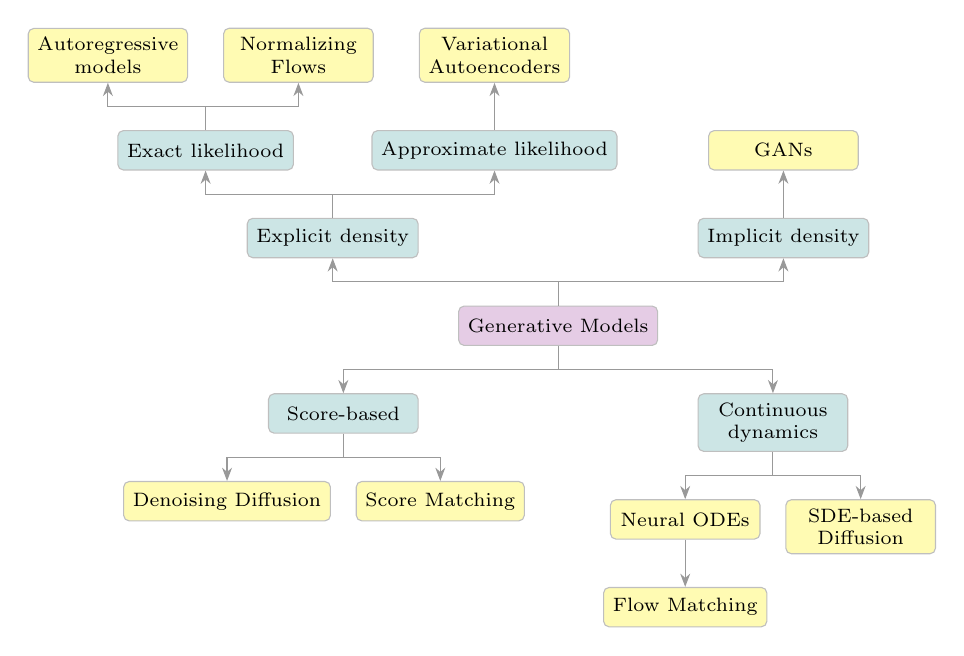
\begin{tikzpicture}[
    scale=1.0, transform shape,
    node distance=0.6cm and 0.3cm,
    box/.style={
        rectangle, 
        draw=gray!50, 
        rounded corners=2pt, 
        minimum width=1.9cm, 
        minimum height=0.5cm, 
        align=center, 
        font=\scriptsize, 
        line width=0.4pt
    },
    root/.style={box, fill=violet!20},
    category/.style={box, fill=teal!20},
    model/.style={box, fill=yellow!30},
    arrow/.style={-Stealth, draw=gray!80, line width=0.4pt}
]

    % --- CENTRAL ROOT ---
    \node[root] (root) {Generative Models};

    % --- UPPER BRANCHES (SWAPPED) ---
    % Tier 1: Explicit (Left) and Implicit (Right)
    \node[category, above left=0.6cm and 0.5cm of root] (explicit) {Explicit density};
    \node[category, above right=0.6cm and 0.5cm of root] (implicit) {Implicit density};

    % Tier 2 (Left side: Likelihoods)
    \node[category, above left=0.6cm and -0.6cm of explicit] (exact) {Exact likelihood};
    \node[category, above right=0.6cm and -0.6cm of explicit] (approx) {Approximate likelihood};

    % Tier 2 (Right side: GANs)
    \node[model, above=0.6cm of implicit] (gans) {GANs};

    % Tier 3 (Final Models Up)
    \node[model, above left=0.6cm and -0.9cm of exact] (ar) {Autoregressive \\ models};
    \node[model, above right=0.6cm and -0.9cm of exact] (nf) {Normalizing \\ Flows};
    \node[model, above=0.6cm of approx] (vae) {Variational \\ Autoencoders};

    % --- LOWER BRANCHES ---
    % Tier 1: Score-based and Continuous
    \node[category, below left=0.6cm and 0.5cm of root] (score) {Score-based};
    \node[category, below right=0.6cm and 0.5cm of root] (cont) {Continuous \\ dynamics};

    % Tier 2 (Score Models)
    \node[model, below left=0.6cm and -0.8cm of score] (ddpm) {Denoising Diffusion};
    \node[model, below right=0.6cm and -0.8cm of score] (sm) {Score Matching};

    % Tier 2 (Continuous Models)
    \node[model, below left=0.6cm and -0.8cm of cont] (node) {Neural ODEs};
    \node[model, below right=0.6cm and -0.8cm of cont] (sde) {SDE-based \\ Diffusion};

    % Tier 3 (Flow Matching)
    \node[model, below=0.6cm of node] (fm) {Flow Matching};

    % --- CONNECTIONS ---
    % Root to Tier 1
    \draw[arrow] (root.north) -- ++(0,0.3) -| (explicit.south);
    \draw[arrow] (root.north) -- ++(0,0.3) -| (implicit.south);
    \draw[arrow] (root.south) -- ++(0,-0.3) -| (score.north);
    \draw[arrow] (root.south) -- ++(0,-0.3) -| (cont.north);

    % Explicit side connections
    \draw[arrow] (explicit.north) -- ++(0,0.3) -| (exact.south);
    \draw[arrow] (explicit.north) -- ++(0,0.3) -| (approx.south);
    \draw[arrow] (exact.north) -- ++(0,0.3) -| (ar.south);
    \draw[arrow] (exact.north) -- ++(0,0.3) -| (nf.south);
    \draw[arrow] (approx.north) -- (vae.south);

    % Implicit side connection
    \draw[arrow] (implicit.north) -- (gans.south);

    % Score side connections
    \draw[arrow] (score.south) -- ++(0,-0.3) -| (ddpm.north);
    \draw[arrow] (score.south) -- ++(0,-0.3) -| (sm.north);

    % Continuous side connections
    \draw[arrow] (cont.south) -- ++(0,-0.3) -| (node.north);
    \draw[arrow] (cont.south) -- ++(0,-0.3) -| (sde.north);
    \draw[arrow] (node.south) -- (fm.north);

\end{tikzpicture}     % Generative models taxonomy diagram

\createdgmtitle{1}

%--------------------------------------------------------------------------------

\usepackage{tikz}
\usetikzlibrary{arrows.meta,positioning,fit}

% Disable slide pausing commands for merged document
\renewcommand{\eqpause}{}
\renewcommand{\nextonslide}[1]{#1}

\begin{document}
%--------------------------------------------------------------------------------

%================================================================================
% LECTURE 1
%================================================================================
\part{Lecture 1}
\createdgmtitle{1}

%--------------------------------------------------------------------------------
\begin{frame}[noframenumbering,plain]
\titlepage
\resetonslide
\end{frame}

%=======
\begin{frame}{Generative Models Zoo}
	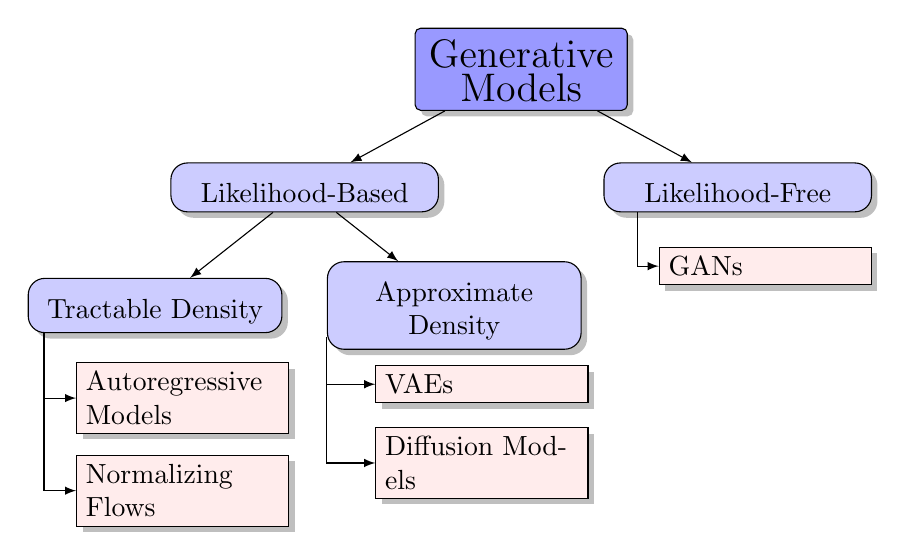
\begin{tikzpicture}[
	 	basic/.style  = {draw, text width=2cm, drop shadow, rectangle},
	 	root/.style   = {basic, rounded corners=2pt, thin, text height=1.1em, text width=7em, align=center, fill=blue!40},
	 	level 1/.style={sibling distance=55mm},
	 	level 2/.style = {basic, rounded corners=6pt, thin, align=center, fill=blue!20, text height=1.1em, text width=9em, sibling distance=38mm},
	 	level 3/.style = {basic, rounded corners=6pt, thin,align=center, fill=blue!20, text width=8.5em},
	 	level 4/.style = {basic, thin, align=left, fill=pink!30, text width=7em},
		edge from parent/.style={->,draw},
		>=latex]
		
		% Root of the tree, level 1
		\node[root] {\Large Generative Models}
		% The first level, as children of the initial tree
		child {node[level 2] (c1) {Likelihood-Based}
			child {node[level 3] (c11) {Tractable Density}}
			child {node[level 3] (c12) {Approximate Density}}
		}
		child {node[level 2] (c2) {Likelihood-Free}};
		
		% Second level, relatively positioned nodes
		\begin{scope}[every node/.style={level 4}]
		\node [below of = c11, yshift=-5pt, xshift=10pt] (c111) {Autoregressive Models};
		\node [below of = c111, yshift=-5pt] (c112) {Normalizing Flows};
		
		\node [below of = c12, xshift=10pt] (c121) {VAEs};
		\node [below of = c121] (c122) {Diffusion Models};
		
		\node [below of = c2, xshift=10pt] (c21) {GANs};
		\end{scope}
		
		% Lines from each level 1 node to every one of its "children"
		\foreach \value in {1,2}
		\draw[->] (c11.194) |- (c11\value.west);
		
		\foreach \value in {1,2}
		\draw[->] (c12.194) |- (c12\value.west);
		
		\draw[->] (c2.194) |- (c21.west);
		
	\end{tikzpicture}
\end{frame}
%=======
\begin{frame}{Outline}
	\tableofcontents[part=1]
\end{frame}
%=======
\section{Generative Models Overview}
%=======
\begin{frame}{VAE -- The First Scalable Approach for Image Generation}
\myfootnotewithlink{https://arxiv.org/abs/1312.6114}{Kingma D.P., Welling M. Auto-Encoding Variational Bayes, 2013}
    \begin{figure}
        \centering
        \includegraphics[width=0.8\linewidth]{../lecture1/figs/vae.png}
    \end{figure}
\end{frame}
%=======
\begin{frame}{DCGAN -- The First Convolutional GAN for Image Generation}
\myfootnotewithlink{https://arxiv.org/abs/1511.06434}{Radford A., Metz L., Chintala S. Unsupervised Representation Learning with Deep Convolutional Generative Adversarial Networks, 2015}
    \begin{figure}
        \centering
        \includegraphics[width=1.0\linewidth]{../lecture1/figs/dcgan.png}
    \end{figure}
\end{frame}
%=======
\begin{frame}{StyleGAN -- High-Quality Face Generation}
	\vspace{-0.2cm}
	\myfootnotewithlink{https://arxiv.org/abs/1812.04948}{Karras T., Laine S., Aila T. A Style-Based Generator Architecture for Generative Adversarial Networks, 2018}
	\begin{figure}
		\centering
		\includegraphics[width=0.85\linewidth]{../lecture1/figs/gan_evolution}
	\end{figure}
	\vspace{-0.5cm}
	\begin{figure}
		\centering
		\includegraphics[width=0.75\linewidth]{../lecture1/figs/stylegan}
	\end{figure}
\end{frame}
%=======
\begin{frame}{Language Modeling at Scale}
	\myfootnotewithlink{https://blog.biocomm.ai/2023/05/14/open-source-proliferation-llm-evolutionary-tree/}{Image credit: https://blog.biocomm.ai/2023/05/14/open-source-proliferation-llm-evolutionary-tree/}
	\begin{figure}
		\includegraphics[width=0.85\linewidth]{../lecture1/figs/LLM-Evolutionary-Tree}
	\end{figure}
\end{frame}
%=======
\begin{frame}{Denoising Diffusion Probabilistic Model}
	\myfootnotewithlink{https://arxiv.org/abs/2105.05233}{Dhariwal P., Nichol A. Diffusion Models Beat GANs on Image Synthesis, 2021}
	\begin{figure}
		\includegraphics[width=\linewidth]{../lecture1/figs/diffusion_models}
	\end{figure}
\end{frame}
%=======
\begin{frame}{Midjourney -- Impressive Text-to-Image Results}
	\myfootnotewithlink{https://www.midjourney.com/explore}{Image credit: https://www.midjourney.com/explore}
	\begin{figure}
		\includegraphics[width=\linewidth]{../lecture1/figs/midjourney}
	\end{figure}
\end{frame}
%=======
\begin{frame}{Sora -- Video Generation}
	\myfootnotewithlink{https://openai.com/index/sora}{Image credit: https://openai.com/index/sora}
	\begin{figure}
		\includegraphics[width=\linewidth]{../lecture1/figs/sora}
	\end{figure}
\end{frame}
%=======
\begin{frame}{GPT4o Image Editing}
	\myfootnotewithlink{https://openai.com/index/introducing-4o-image-generation/}{Image credit: https://openai.com/index/introducing-4o-image-generation/}
	\textbf{Prompt:} Give this cat a detective hat and a monocle
	\begin{minipage}[t]{0.5\columnwidth}		
		\begin{figure}
			\includegraphics[width=0.94\linewidth]{../lecture1/figs/gpt4o_editing1}
		\end{figure}
	\end{minipage}%
	\begin{minipage}[t]{0.45\columnwidth}		
		\begin{figure}
			\includegraphics[width=0.93\linewidth]{../lecture1/figs/gpt4o_editing2}
		\end{figure}
	\end{minipage}
\end{frame}
%=======
\begin{frame}{Open Problems in Generative Models}
	\myfootnotewithlink{https://arxiv.org/abs/2501.09038}{Motamed S. et al. Do generative video models understand physical principles?, 2025}
	\begin{itemize}
		\item Video generation
		\item 3D scene generation
		\item Understanding of physical processes
		\item Multimodal end-to-end models
	\end{itemize}	
	\begin{figure}
		\includegraphics[width=0.55\linewidth]{../lecture1/figs/physics_understand}
	\end{figure}
\end{frame}
%=======
\section{Course Tricks}
%=======
\begin{frame}{Course Tricks I}
	\begin{block}{Log-Derivative Trick}
		Given a differentiable function $p: \bbR^m \to \bbR$ (usually density function),
		$$
			\nabla \log p(\bx) = \frac{1}{p(\bx)} \cdot \nabla p(\bx).
		$$
		\vspace{-0.5cm}
	\end{block}
    \eqpause
	\begin{block}{Jensen's Inequality}
		If $\bx \in \bbR^m$ is a continuous random variable with density $p(\bx)$ and $f: \bbR^m \to \bbR$ is convex, then
		$$
			\bbE[f(\bx)] \geq f(\bbE[\bx]).
		$$
		\vspace{-0.7cm}
	\end{block}
    \eqpause
	\begin{block}{Monte Carlo Estimation}
		Let $\bx \in \bbR^m$ be a continuous random variable with density $p(\bx)$, and $\bff: \bbR^m \to \bbR^d$ be any vector-valued function. Then,
		$$
			\bbE_{p(\bx)} \bff(\bx) = \int p(\bx) \bff(\bx) d \bx \approx \frac{1}{n} \sum_{i=1}^n \bff(\bx_i), \quad 
			\text{where } \bx_i \sim p(\bx).
		$$
		\vspace{-0.4cm}
	\end{block}
\end{frame}
%=======
\begin{frame}{Course Tricks II}
	\begin{block}{Change of Variables Theorem (CoV)}
		Let $\bx\in \bbR^m$ be a random vector with density $p(\bx)$, and let $\bff: \bbR^m \rightarrow \bbR^m$ be a $C^1$-diffeomorphism ($\bff$ and $\bff^{-1}$ are continuously differentiable mappings). 
		If $\bz = \bff(\bx)$, then
		\begin{align*}
			p(\bx) &= p(\bz) |\det(\bJ_{\bff})| = p(\bz) \left|\det \left( \frac{\partial \bz}{\partial \bx} \right) \right| 
			\nextonslide{= p(\bff(\bx)) \left|\det \left(  \frac{\partial \bff(\bx)}{\partial \bx} \right) \right|} \\
			\nextonslide{p(\bz) &= p(\bx) |\det(\bJ_{\bff^{-1}})| = p(\bx) \left|\det \left(  \frac{\partial \bx}{\partial \bz} \right) \right| 
			= p(\bff^{-1}(\bz)) \left|\det \left(  \frac{\partial \bff^{-1}(\bz)}{\partial \bz} \right) \right| }
		\end{align*}
		\vspace{-0.5cm}
	\end{block}
    \eqpause
	\begin{block}{Proof (1D)}
		Assume $f$ is monotonically increasing.
		\[
			F_Y(y) = P(Y \leq y) = P(x \leq f^{-1}(y)) = F_X(f^{-1}(y))
		\]
        \eqpause
		\vspace{-0.3cm}
		$$
			p(y) = \frac{dF_Y(y)}{dy} = \frac{dF_X(f^{-1}(y))}{dy} = \frac{dF_X(x)}{dx} \frac{df^{-1}(y)}{dy} =  p(x) \frac{df^{-1}(y)}{dy}
		$$
	\end{block}
\end{frame}
%=======
\begin{frame}{Course Tricks III}
	\begin{block}{Law of the Unconscious Statistician (LOTUS)}
		Let $\bx \in \bbR^m$ be a continuous random variable with density $p(\bx)$, and let $\bff: \bbR^m \to \bbR^m$ be measurable. If $\by = \bff(\bx)$, then
		$$
			\bbE_{p(\by)} \bg(\by) = \int p(\by) \bg(\by) d\by \nextonslide{= \int p(\bx) \bg(\bff(\bx)) d\bx = \bbE_{p(\bx)} \bg(\bff(\bx))}.
		$$
		\vspace{-0.4cm}
	\end{block}
    \eqpause
	\begin{block}{Dirac Delta Function}
		Any deterministic variable $\bx_0$ can be interpreted as a random variable with density $p(\bx) = \delta(\bx - \bx_0)$. 
		\vspace{-0.3cm}
		$$
			\delta(\bx) = 
			\begin{cases}
				+\infty, & \bx = 0 \\
				0, & \bx \neq 0
			\end{cases} \qquad 
			\int \delta(\bx) d\bx = 1
		$$
        \eqpause
		$$
			\bbE_{p(\bx)}\bff(\bx) = \int \delta (\bx - \bx_0) \bff(\bx) d\bx = \bff(\bx_0)
		$$
	\end{block}
\end{frame}
%=======
\section{Problem Statement}
%=======
\begin{frame}{Problem Statement}
	We're given \textbf{finite} number of i.i.d.\ samples $\{\bx_i\}_{i=1}^n \subset \bbR^m$ drawn from an \textbf{unknown} distribution $\pd(\bx)$.
	\eqpause
	\begin{block}{Objective}
		Our aim is to learn a distribution $\pd(\bx)$ that allows us to: 
		\begin{itemize}
		    \item Generate new samples from $\pd(\bx)$ (sample $\bx \sim \pd(\bx)$) --- \textbf{generation}.		    
			\eqpause
		    \item Evaluate $\pd(\bx)$ on novel data (answering ``How likely is an object $\bx$?'') --- \textbf{density estimation}; 
		\end{itemize}
	\end{block}
	\eqpause
	\begin{block}{Challenge}
		The data is high-dimensional and complex. For example, image datasets live in $\bbR^{\text{width} \times \text{height} \times \text{channels}}$. The curse of dimensionality makes accurately estimating $\pd(\bx)$ infeasible.
	\end{block}
	\eqpause
	\textbf{Note:} here we use a strong assumption that our data is continuous (thus avoiding the domain of texts).
\end{frame}
%=======
\begin{frame}{Histogram as a Generative Model}
	
	\begin{minipage}[t]{0.6\columnwidth}
	    Assume $x \sim \Cat(\bpi)$. The histogram model is fully characterized by
		$$
		    \hat{\pi}_k = \hat{\pi}(x = k) = \frac{\sum_{i=1}^n [x_i = k]}{n}.
		$$
		\textbf{Curse of dimensionality:} The number of bins rises exponentially. \\
	\end{minipage}%
	\begin{minipage}[t]{0.4\columnwidth}
		\vspace{-0.5cm}
	    \begin{figure}[h]
	        \centering
	        \includegraphics[width=\linewidth]{../lecture1/figs/histogram.png}
	    \end{figure}
	\end{minipage}
    \eqpause
	\textbf{MNIST example}: $28 \times 28$ grayscale images, with each image $\bx = (x_1, \dots, x_{784})$, $x_i \in \{0, 1\}$:
	$$
	    \pd(\bx) = p(x_1) \cdot p(x_2 | x_1) \cdot \dots \cdot p(x_m | x_{m-1}, \dots, x_1).
	$$
    \eqpause
	A complete histogram would require $2^{28 \times 28} - 1$ parameters for~$\pd(\bx)$.\\
    \eqpause
	\textbf{Question:} How many parameters are required in these cases?
	\begin{align*}
	    \pd(\bx) &= p(x_1) \cdot p(x_2)\cdot \dots \cdot p(x_m); \\
	    \pd(\bx) &= p(x_1) \cdot p(x_2 | x_1) \cdot \dots \cdot p(x_m | x_{m-1}).
	\end{align*}
\end{frame}
%=======
\begin{frame}{ Conditional Models}
	In practice, we're typically interested in learning conditional models (sampling from conditional distribution~$\pd(\bx | \by)$). 
	\eqpause
	\begin{itemize}
		\item $\by = \emptyset$, $\bx$ = image $\quad\Rightarrow\quad$ unconditional image model
		\item $\by$ = class label, $\bx$ = image $\quad\Rightarrow\quad$ class-conditional image model
		\item $\by$ = text prompt, $\bx$ = image $\quad\Rightarrow\quad$ text-to-image model
		\item $\by$ = image, $\bx$ = image $\quad\Rightarrow\quad$ image-to-image model
		\item $\by$ = image, $\bx$ = text $\quad\Rightarrow\quad$ image-to-text (image captioning) model
		\item $\by$ = English text, $\bx$ = Russian text $\quad\Rightarrow\quad$ sequence-to-sequence model (machine translation) model
		\item $\by$ = sound, $\bx$ = text $\quad\Rightarrow\quad$ speech-to-text (automatic speech recognition) model
		\item $\by$ = text, $\bx$ = sound $\quad\Rightarrow\quad$ text-to-speech model
	\end{itemize}
\end{frame}
%=======
\section{Divergence Minimization Framework}
%=======
\begin{frame}{Divergences}
	\begin{itemize}
	\item Let us fix a probabilistic model $\pt(\bx)$ from a parametric family of distributions $\{p(\bx | \btheta) \, | \, \btheta \in \bTheta\}$.\\
        \eqpause
	\item Instead of searching among all possible distributions for the true $\pd(\bx)$, we seek a functional approximation $\pt(\bx) \approx \pd(\bx)$.
	\end{itemize}
    \eqpause
	\begin{block}{What is a Divergence?}
		Let $\cP$ be the set of all probability distributions. A mapping $D: \cP \times \cP \to \bbR$ is called a \textbf{divergence} if 
		\begin{itemize}
			\item $D(\pi \| p) \geq 0$ for all $\pi, p \in \cP$
			\item $D(\pi \| p) = 0$ if and only if $\pi \equiv p$
		\end{itemize}
	\end{block}
    \eqpause
	\begin{block}{Divergence Minimization Problem}
		\vspace{-0.3cm}
		$$
		\min_{\btheta} D(\pd \| \pt)
		$$
		where $\pd(\bx)$ is the true data distribution and $\pt(\bx)$ is the model distribution.
	\end{block}
\end{frame}
%=======
\begin{frame}{Forward KL vs Reverse KL (Kullback-Leibler Divergence)}
	\begin{block}{Forward KL}
		\vspace{-0.2cm}
		\[
			\KL(\pd \| \pt) = \int \pd(\bx) \log \frac{\pd(\bx)}{\pt(\bx)} d \bx \rightarrow \min_{\btheta}
		\]
	\end{block}
    \eqpause
	\begin{block}{Reverse KL}
		\vspace{-0.2cm}
		\[
			\KL(\pt \| \pd) = \int \pt(\bx) \log \frac{\pt(\bx)}{\pd(\bx)} d \bx \rightarrow \min_{\btheta}
		\]
	\end{block}
    \eqpause
	What's the practical distinction between these two objectives?
    \eqpause
	\begin{block}{Maximum Likelihood Estimation (MLE)}
	Let $\{\bx_i\}_{i=1}^n$ be i.i.d.\ observed samples.
		\vspace{-0.3cm}
		\[
			\btheta^* = \argmax_{\btheta} \prod_{i=1}^n \pt(\bx_i) = \argmax_{\btheta} \sum_{i=1}^n \log \pt(\bx_i).
		\]
	\end{block}
\end{frame}
%=======
\begin{frame}{Forward KL vs Reverse KL: MLE as Forward KL}
	\begin{block}{Forward KL}
		\vspace{-0.5cm}
		\begin{align*}
			\KL(\pd \| \pt) &= \int \pd(\bx) \log \frac{\pd(\bx)}{\pt(\bx)} d\bx \\
			\nextonslide{&= {\color{violet}\int \pd(\bx) \log \pd(\bx) d \bx} - {\color{teal}\int \pd(\bx) \log \pt(\bx) d \bx}} \\
			\nextonslide{&= -{\color{teal}\bbE_{\pd(\bx)} [\log \pt(\bx)]} + {\color{violet}\text{const}}} \\
			\nextonslide{& \approx - \frac{1}{n} \sum_{i=1}^n \log \pt(\bx_i) + \text{const} \rightarrow \min_{\btheta}.}
		\end{align*}
		\vspace{-0.5cm}
	\end{block}
	\eqpause
	Maximum likelihood estimation is thus equivalent to minimizing a Monte Carlo estimate of the forward KL divergence.
    \eqpause
	\begin{block}{Reverse KL}
		\vspace{-0.5cm}
		\begin{align*}
			\KL(\pt \| \pd) &= \int \pt(\bx) \log \frac{\pt(\bx)}{\pd(\bx)} d \bx \\
			\nextonslide{&= \bbE_{\pt(\bx)} \left[\log \pt(\bx) - \log \pd(\bx)\right] \rightarrow \min_{\btheta}}
		\end{align*}
		\vspace{-0.7cm}
	\end{block}
\end{frame}
%=======
\section{Autoregressive Modeling}
%=======
\begin{frame}{Generative Models Zoo}
	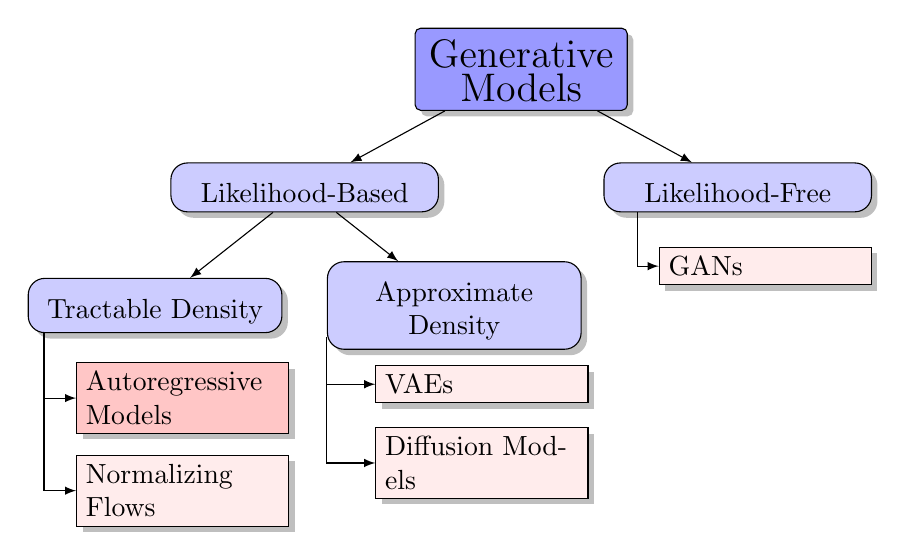
\begin{tikzpicture}[
		basic/.style  = {draw, text width=2cm, drop shadow, rectangle},
		root/.style   = {basic, rounded corners=2pt, thin, text height=1.1em, text width=7em, align=center, fill=blue!40},
		level 1/.style={sibling distance=55mm},
		level 2/.style = {basic, rounded corners=6pt, thin, align=center, fill=blue!20, text height=1.1em, text width=9em, sibling distance=38mm},
		level 3/.style = {basic, rounded corners=6pt, thin,align=center, fill=blue!20, text width=8.5em},
		level 4/.style = {basic, thin, align=left, fill=pink!30, text width=7em},
		level 5/.style = {basic, thin, align=left, fill=pink!90, text width=7em},
		edge from parent/.style={->,draw},
		>=latex]
		
		% Root of initial tree, level 1
		\node[root] {\Large Generative Models}
		% The first level, as children of the initial tree
		child {node[level 2] (c1) {Likelihood-Based}
			child {node[level 3] (c11) {Tractable Density}}
			child {node[level 3] (c12) {Approximate Density}}
		}
		child {node[level 2] (c2) {Likelihood-Free}};
		
		% Second level, relatively positioned nodes
		\begin{scope}[every node/.style={level 5}]
			\node [below of = c11, yshift=-5pt, xshift=10pt] (c111) {Autoregressive Models};
		\end{scope}
		
		% Second level, relatively positioned nodes
		\begin{scope}[every node/.style={level 4}]
			\node [below of = c111, yshift=-5pt] (c112) {Normalizing Flows};
			
			\node [below of = c12, xshift=10pt] (c121) {VAEs};
			\node [below of = c121] (c122) {Diffusion Models};
			
			\node [below of = c2, xshift=10pt] (c21) {GANs};
		\end{scope}
		
		% Lines from each level 1 node to every one of its "children"
		\foreach \value in {1,2}
		\draw[->] (c11.194) |- (c11\value.west);
		
		\foreach \value in {1,2}
		\draw[->] (c12.194) |- (c12\value.west);
		
		\draw[->] (c2.194) |- (c21.west);
		
	\end{tikzpicture}
\end{frame}
%=======
\begin{frame}{Autoregressive Modeling}
    \begin{block}{MLE Problem}
	    \vspace{-0.4cm}
	    $$
	        \btheta^* = \argmax_{\btheta} \prod_{i=1}^n \pt(\bx_i) = \argmax_{\btheta} \sum_{i=1}^n \log \pt(\bx_i)
	    $$
	    \vspace{-0.5cm}
    \end{block}
    \eqpause
    \begin{itemize}
        \item This maximization is typically solved via gradient-based optimization.
        \item Thus, efficient computation of both $\log \pt(\bx)$ and its gradient $\frac{\partial \log \pt(\bx)}{\partial \btheta}$ is crucial.
    \end{itemize}
    \eqpause
    \begin{block}{Likelihood as a Product of Conditionals}
    For $\bx = (x_1, \dots, x_m)$, $\bx_{1:j} = (x_1, \dots, x_j)$,
    $$
        \pt(\bx) = \prod_{j=1}^m \pt(x_j | \bx_{1:j - 1});\quad
        \log \pt(\bx) = {\color{violet}\sum_{j=1}^m \log \pt(x_j | \bx_{1:j - 1})}
    $$
    \end{block}
    \eqpause
    \vspace{-0.5cm}
	 $$
	     \btheta^* =  \argmax_{\btheta} \sum_{i=1}^n \Big[{\color{violet} \sum_{j=1}^m \log \pt(x_{ij} | \bx_{i, 1:j - 1})}\Big]
	 $$
\end{frame}
%=======
\begin{frame}{Autoregressive Models}
    \[
    	\log \pt(\bx) = \sum_{j=1}^m \log \pt(x_j | \bx_{1:j - 1})
    \]
    \eqpause
    \begin{itemize}
	    \item Sampling is performed sequentially:
	    \begin{itemize}
    		\item Sample $\hat{x}_1 \sim \pt(x_1)$;
    		\item Sample $\hat{x}_2 \sim \pt(x_2 | \hat{x}_1)$;
    		\item $\ldots$
    		\item Sample $\hat{x}_m \sim \pt(x_m | \hat{\bx}_{1:m-1})$;
    		\item The generated sample is $\hat{\bx} = (\hat{x}_1, \hat{x}_2, \ldots, \hat{x}_m)$.
    	\end{itemize}
        \eqpause
        \item Each conditional $\pt(x_j | \bx_{1:j - 1})$ can be modeled using a neural network.
        \eqpause
        \item Modeling all conditionals separately isn't feasible. To address this, we share parameters across all conditionals.
    \end{itemize}
\end{frame}
%=======
\begin{frame}{Autoregressive Models: MLP}
	\myfootnotewithlink{https://jmtomczak.github.io/blog/2/2\_ARM.html}{Image credit: https://jmtomczak.github.io/blog/2/2\_ARM.html}
	For large $j$, the conditional $\pt(x_j | \bx_{1:j - 1})$ becomes intractable as the history $\bx_{1:j-1}$ grows variable-length.
    \eqpause
	\begin{block}{Markov Assumption}
		\vspace{-0.3cm}
		$$
			\pt(x_j | \bx_{1:j - 1}) = \pt(x_j | \bx_{j - d:j - 1}),\quad d\;\text{is a fixed parameter}.
		$$
	\end{block}
    \eqpause
	\vspace{-0.5cm}
	\begin{block}{Example}
		\begin{minipage}[t]{0.39\columnwidth}
			{\small
			\begin{itemize}
				\item $d = 2$
				\item $x_j \in \{0, 255\}$
				\item $\bh_j = \MLP_{\btheta}(x_{j - 1}, x_{j - 2})$
				\item $\bpi_j = \softmax(\bh_j)$
				\item $\pt(x_j | x_{j - 1}, x_{j - 2}) = \Cat(\bpi_j)$
			\end{itemize}
			}
		\end{minipage}%
		\begin{minipage}[t]{0.61\columnwidth}
			 \begin{figure}
			   \centering
			   \includegraphics[width=1.0\linewidth]{../lecture1/figs/sequential_MLP}
			 \end{figure}
			 \eqpause
			 Can we also model continuous-valued data, not just the discrete case?
		\end{minipage}
	\end{block}
\end{frame}
%=======
\begin{frame}{Autoregressive Models: LLM}
	\myfootnotewithlink{https://jmtomczak.github.io/blog/20/20\_llms.html}{Image credit: https://jmtomczak.github.io/blog/20/20\_llms.html}
	\[
		\pt(x_j | \bx_{1:j - 1}) = \pt(x_j | \bx_{j - d:j - 1}),\quad d\ \text{is the context window}.
	\]
	 \begin{figure}
		   \centering
		   \includegraphics[width=1.0\linewidth]{../lecture1/figs/llm_modeling}
	 \end{figure}
\end{frame}
%=======
\begin{frame}{Autoregressive Models for Images}
	\myfootnotewithlink{https://arxiv.org/abs/1601.06759}{Oord A., Kalchbrenner N., Kavukcuoglu K. Pixel Recurrent Neural Networks, 2016}
	How do we model the distribution $\pd(\bx)$ of natural images?
	$$
  		\pt(\bx) = \prod_{j=1}^{\text{width} \times \text{height}} \pt(x_j | \bx_{1:j-1})
	$$
    \eqpause
	\begin{minipage}[t]{0.5\columnwidth}
		\vspace{0.5cm}
		\begin{itemize}
			\item A pixel ordering must be selected; the raster scan is a standard choice.
			\vfill
		    \item RGB channel dependencies can be modeled explicitly as well.
		\end{itemize}
	\end{minipage}%
	\begin{minipage}[t]{0.5\columnwidth}
		\begin{figure}
			\centering
   			\includegraphics[width=0.9\linewidth]{../lecture1/figs/pixelcnn1.png}
		\end{figure}
	\end{minipage}
\end{frame}
%=======
\begin{frame}{Autoregressive Models: ImageGPT}
	\myfootnotewithlink{https://cdn.openai.com/papers/Generative_Pretraining_from_Pixels_V2.pdf}{Chen M. et al. Generative Pretraining from Pixels, 2020}
	\begin{figure}
		\centering
  			\includegraphics[width=0.65\linewidth]{../lecture1/figs/imagegpt.png}
	\end{figure}
\end{frame}
%=======
\begin{frame}{Summary}
    \begin{itemize}
    	\item Our target is to approximate the data distribution both for density estimation and for generation.
    	\vfill
    	\item The divergence minimization framework offers a principled way to learn distributions that match the data.
    	\vfill
    	\item Minimizing the forward KL divergence is equivalent to maximum likelihood estimation.
    	\vfill
    	\item Autoregressive models decompose the joint distribution as a product of conditionals.
    	\vfill
        \item Autoregressive sampling is simple, but inherently sequential.
        \vfill
        \item Joint density evaluation multiplies all conditional probabilities $\pt(x_j | \bx_{1:j - 1})$.
        \vfill
     	\item ImageGPT applies a transformer architecture to sequences of raster-ordered image pixels.
    \end{itemize}
\end{frame}


%================================================================================
% LECTURE 2
%================================================================================
\part{Lecture 2}
\createdgmtitle{2}

%--------------------------------------------------------------------------------
\begin{frame}[noframenumbering,plain]
\titlepage
\resetonslide
\end{frame}




%=======
\begin{frame}{Outline}
	\tableofcontents[part=2]
\end{frame}
%=======
\section{Normalizing Flows (NF)}
%=======
\begin{frame}{Generative Models Zoo}
	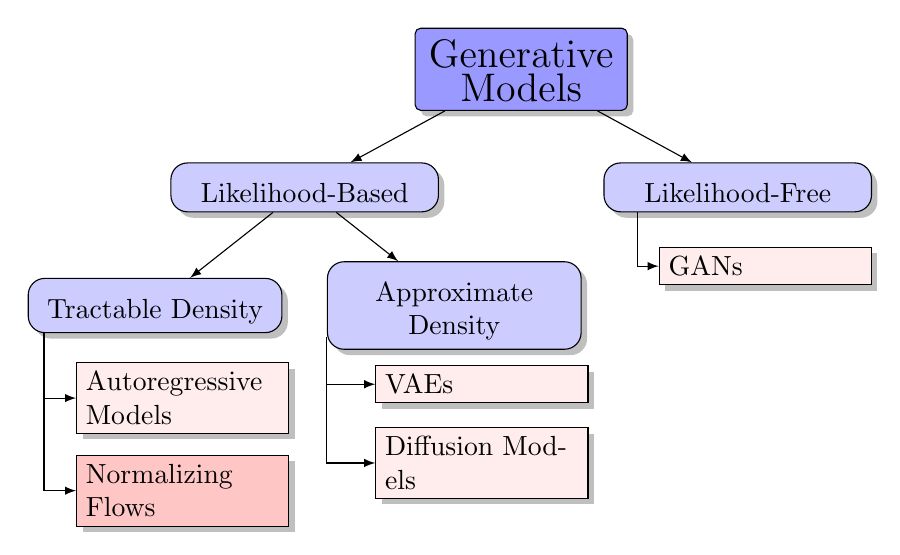
\begin{tikzpicture}[
	 	basic/.style  = {draw, text width=2cm, drop shadow, rectangle},
	 	root/.style   = {basic, rounded corners=2pt, thin, text height=1.1em, text width=7em, align=center, fill=blue!40},
	 	level 1/.style={sibling distance=55mm},
	 	level 2/.style = {basic, rounded corners=6pt, thin, align=center, fill=blue!20, text height=1.1em, text width=9em, sibling distance=38mm},
	 	level 3/.style = {basic, rounded corners=6pt, thin,align=center, fill=blue!20, text width=8.5em},
	 	level 4/.style = {basic, thin, align=left, fill=pink!30, text width=7em},
	 	level 5/.style = {basic, thin, align=left, fill=pink!90, text width=7em},
		edge from parent/.style={->,draw},
		>=latex]
		
		% root of the initial tree, level 1
		\node[root] {\Large Generative Models}
		% The first level, as children of the initial tree
		child {node[level 2] (c1) {Likelihood-Based}
			child {node[level 3] (c11) {Tractable Density}}
			child {node[level 3] (c12) {Approximate Density}}
		}
		child {node[level 2] (c2) {Likelihood-Free}};
		
		% The second level, relatively positioned nodes
		\begin{scope}[every node/.style={level 4}]
		\node [below of = c11, yshift=-5pt, xshift=10pt] (c111) {Autoregressive Models};
		
		\node [below of = c12, xshift=10pt] (c121) {VAEs};
		\node [below of = c121] (c122) {Diffusion Models};
		\node [below of = c2, xshift=10pt] (c21) {GANs};
		
		\end{scope}
		
		% The second level, relatively positioned nodes
		\begin{scope}[every node/.style={level 5}]
			\node [below of = c111, yshift=-5pt] (c112) {Normalizing Flows};
		\end{scope}
		
		
		% lines from each level 1 node to every one of its "children"
		\foreach \value in {1,2}
		\draw[->] (c11.194) |- (c11\value.west);
		
		\foreach \value in {1,2}
		\draw[->] (c12.194) |- (c12\value.west);
		
		\draw[->] (c2.194) |- (c21.west);
		
	\end{tikzpicture}
\end{frame}
%=======
\begin{frame}{Normalizing Flows: Prerequisites}
	\begin{block}{Jacobian Matrix}
		Let $\bff: \bbR^m \rightarrow \bbR^m$ be a differentiable function.
		\[
			\bz = \bff(\bx), \quad 
			\bJ =  \frac{\partial \bz}{\partial \bx} =
			\begin{pmatrix}
				\frac{\partial z_1}{\partial x_1} & \dots & \frac{\partial z_1}{\partial x_m} \\
				\vdots & \ddots & \vdots \\ 
				\frac{\partial z_m}{\partial x_1} & \dots & \frac{\partial z_m}{\partial x_m}
			\end{pmatrix} \in \bbR^{m \times m}
		\]
		\vspace{-0.3cm}
	\end{block}
    \eqpause
	\begin{block}{Change of Variables Theorem (CoV)}
		Let $\bx\in \bbR^m$ be a random vector with density $p(\bx)$, and let $\bff: \bbR^m \rightarrow \bbR^m$ be a $C^1$-diffeomorphism ($\bff$ and $\bff^{-1}$ are continuously differentiable mappings). 
		If $\bz = \bff(\bx)$, then
		\begin{align*}
			p(\bx) &= p(\bz) |\det(\bJ_{\bff})| = p(\bz) \left|\det \left( \frac{\partial \bz}{\partial \bx} \right) \right| 
			\nextonslide{= p(\bff(\bx)) \left|\det \left(  \frac{\partial \bff(\bx)}{\partial \bx} \right) \right|} \\
			\nextonslide{p(\bz) &= p(\bx) |\det(\bJ_{\bff^{-1}})| = p(\bx) \left|\det \left(  \frac{\partial \bx}{\partial \bz} \right) \right| 
			= p(\bff^{-1}(\bz)) \left|\det \left(  \frac{\partial \bff^{-1}(\bz)}{\partial \bz} \right) \right| }
		\end{align*}
		\vspace{-0.5cm}
	\end{block}
\end{frame}
%=======
\begin{frame}{Jacobian Determinant}
	\myfootnotewithlink{https://jmtomczak.github.io/blog/3/3\_flows.html}{https://jmtomczak.github.io/blog/3/3\_flows.html}
	\begin{block}{Inverse Function Theorem}
		If the function $\bff$ is invertible and its Jacobian is continuous and non-singular, then
		\vspace{-0.3cm}
		\[
		\bJ_{\bff^{-1}} = \bJ_\bff^{-1}; \quad \nextonslide{|\det (\bJ_{\bff^{-1}})| = \frac{1}{|\det (\bJ_\bff)|}}
		\]
		\vspace{-0.3cm}
	\end{block}
    \eqpause
	\begin{minipage}{0.55\columnwidth}
		\begin{itemize}
			\item $\bx$ and $\bz$ reside in the same space ($\bbR^m$).
			\vfill
			\item $\bff_{\btheta}(\bx)$ is a parameterized transformation.
			\vfill
			\eqpause
			\item The determinant of the Jacobian $\bJ =\frac{\partial \bff_{\btheta}(\bx)}{\partial \bx}$ quantifies how the volume is changed by the transformation.
		\end{itemize}
	\end{minipage}%
	\begin{minipage}{0.45\columnwidth}
		\begin{figure}
			\includegraphics[width=0.8\linewidth]{../lecture2/figs/jacobian_det}
		\end{figure}
	\end{minipage}
\end{frame}
%=======
\begin{frame}{Fitting Normalizing Flows}
	\myfootnotewithlink{https://arxiv.org/abs/1605.08803}{Dinh L., Sohl-Dickstein J., Bengio S. Density Estimation Using Real NVP, 2016} 
	\begin{block}{MLE Problem}
		\vspace{-0.5cm}
		\begin{align*}
			\pt(\bx) &= p(\bz) \left|\det \left(  \frac{\partial \bz}{\partial \bx} \right) \right|  = p(\bff_{\btheta}(\bx)) \left|\det \left( \frac{\partial \bff_{\btheta}(\bx)}{\partial \bx} \right) \right| \\ 
			\nextonslide{\log \pt(\bx) &= \log p(\bff_{\btheta}(\bx)) + \log  |\det (\bJ_{\bff}) | \rightarrow \max_{\btheta}
			}
		\end{align*}
	\end{block}
    \eqpause
	\vspace{-0.2cm}
	\begin{figure}
		\includegraphics[width=0.85\linewidth]{../lecture2/figs/flows_how2}
	\end{figure}
\end{frame}
%=======
\begin{frame}{Composition of Normalizing Flows}
	\myfootnotewithlink{https://lilianweng.github.io/lil-log/2018/10/13/flow-based-deep-generative-models.html}{https://lilianweng.github.io/lil-log/2018/10/13/flow-based-deep-generative-models.html}
	\vspace{-0.3cm}
	\begin{figure}
		\includegraphics[width=0.95\linewidth]{../lecture2/figs/normalizing-flow}
	\end{figure}
	\vspace{-0.3cm}
	\eqpause
	\begin{block}{Theorem}
		If every $\{\bff_k\}_{k=1}^K$ satisfies the conditions of the change-of-variables theorem, then the composition $\bff(\bx) = \bff_K \circ \ldots \circ \bff_1(\bx)$ also satisfies them.
	\end{block}
	\vspace{-0.3cm}
	{\footnotesize
		\begin{multline*}
			\pt(\bx) = p(\bff(\bx)) \left|\det \left(\frac{\partial \bff(\bx)}{\partial \bx} \right) \right| 
			\nextonslide{=p(\bff(\bx)) \left|\det \left(\frac{\partial \bff_K}{\partial \bff_{K-1}} \dots \frac{\partial \bff_1}{\partial \bx} \right) \right|}
			\nextonslide{= \\ = p(\bff(\bx)) \prod_{k=1}^K \left|\det \left(\frac{\partial \bff_{k}}{\partial \bff_{k-1}} \right) \right|
			= p(\bff(\bx)) \prod_{k=1}^K |\det ( \bJ_{\bff_k}) |}
		\end{multline*}
	}
\end{frame}
%=======
\begin{frame}{Normalizing Flows (NF)}
	\vspace{-0.3cm}
	\[
		\log \pt(\bx) = \log p(\bff_{\btheta}(\bx)) + \log |\det (\bJ_\bff)|
	\]
	\vspace{-0.4cm}
	\begin{block}{Definition}
		A normalizing flow is a $C^1$-diffeomorphism that transforms data $\bx$ to noise $\bz$.
	\end{block}
    \eqpause
	\begin{itemize}
		\item \textbf{Normalizing} refers to mapping samples from $\pd(\bx)$ to a base distribution $p(\bz)$.
		\item \textbf{Flow} describes the sequence of transformations that maps samples from $p(\bz)$ to the target, more complex distribution.
		\[
			\bz = \bff_K \circ \ldots \circ \bff_1(\bx); \quad \bx = \bff_1^{-1} \circ \ldots \circ \bff_K^{-1} (\bz)
		\] 
		\vspace{-0.4cm}
		\eqpause
		\begin{block}{Log-Likelihood}
			\vspace{-0.5cm}
			\[
				\log \pt(\bx) = \log p(\bff_K \circ \ldots \circ \bff_1(\bx)) + \sum_{k=1}^K \log |\det (\bJ_{\bff_k})|
			\]
			\vspace{-0.4cm} \\
			where $\bJ_{\bff_k} = \frac{\partial \bff_k}{\partial \bff_{k-1}}$.
		\end{block}
	\end{itemize}
	\eqpause
	\textbf{Note:} Here we consider only \textbf{continuous} random variables.
\end{frame}
%=======
\begin{frame}{Normalizing Flows}
	\myfootnotewithlink{https://arxiv.org/abs/1912.02762}{Papamakarios G. et al. Normalizing Flows for Probabilistic Modeling and Inference, 2019} 
	\begin{block}{Example: 4-Step NF}
		\vspace{-0.2cm}
		\begin{figure}
			\includegraphics[width=\linewidth]{../lecture2/figs/flow_4_steps_example.png}
		\end{figure}
	\end{block}
    \eqpause
	\vspace{-0.5cm}
	\begin{block}{NF Log-Likelihood}
		\vspace{-0.3cm}
		\[
			\log \pt(\bx) = \log p(\bff_{\btheta}(\bx)) + \log |\det ( \bJ_\bff)|
		\]
		\vspace{-0.5cm}
	\end{block}
	What's the computational complexity of evaluating this determinant?
    \eqpause
	\begin{block}{Requirements}
		\begin{itemize}
			\item Efficient computation of the Jacobian $\bJ_\bff = \frac{\partial \bff_{\btheta}(\bx)}{\partial \bx}$
			\item Efficient inversion of the transformation $\bff_{\btheta}(\bx)$
		\end{itemize}
	\end{block}
\end{frame}
%=======
\section{NF Examples}
%=======
\subsection{Linear Normalizing Flows}
%=======
\begin{frame}{Jacobian Structure}
	\begin{block}{Normalizing Flows Log-Likelihood}
		\[
			\log \pt(\bx) = \log p(\bff_{\btheta}(\bx)) + \log \left|\det \left( \frac{\partial \bff_{\btheta}(\bx)}{\partial \bx} \right) \right|
		\]
	\end{block}
	The principal computational challenge is evaluating the Jacobian determinant.
    \eqpause
	\begin{block}{What is $\det(\bJ)$ in These Cases?}
		Consider a linear layer $\bz = \bW \bx$, $\bW \in \bbR^{m \times m}$.
		\begin{enumerate}
			\item $\bz$ is a permutation of $\bx$.
			    \eqpause
			\item $z_j$ depends only on $x_j$. 
			\vspace{-0.3cm}
			\[
				\nextonslide{\log \left|\det \left( \frac{\partial \bff_{\btheta}(\bx)}{\partial \bx} \right) \right| = \log \left| \prod_{j=1}^m \frac{\partial f_{j, \btheta}(x_j)}{\partial x_j} \right| = \sum_{j=1}^m \log \left|  \frac{\partial f_{j, \btheta}(x_j)}{\partial x_j} \right|}
			\]
			\vspace{-0.3cm}
			\eqpause
			\item $z_j$ depends only on $\bx_{1:j}$ (autoregressive dependency).
		\end{enumerate}
	\end{block}
\end{frame}
%=======
\begin{frame}{Linear Normalizing Flows}
	\myfootnotewithlink{https://arxiv.org/abs/1912.02762}{Papamakarios G. et al. Normalizing Flows for Probabilistic Modeling and Inference, 2019} 
	\[
		\bz = \bff_{\btheta}(\bx) = \bW \bx, \quad \bW \in \bbR^{m \times m}, \quad \btheta = \bW, \quad \bJ_\bff = \bW^\top
	\]
	In general, matrix inversion has computational complexity $O(m^3)$.
    \eqpause
	\begin{block}{Invertibility}
		\begin{itemize}
			\item Diagonal matrix: $O(m)$.
			\item Triangular matrix: $O(m^2)$.
			\item Directly parameterizing all invertible matrices in a continuous way is infeasible \\ (there is not surjective function from $\bbR^{m^2}$ to the set of all invertible matrices of size $m \times m$).
		\end{itemize}
	\end{block}
\end{frame}
%=======
\begin{frame}{Linear Normalizing Flows}
	\myfootnote{\href{https://arxiv.org/abs/1807.03039}{Kingma D. P., et al. Glow: Generative Flow with Invertible 1x1 Convolutions, 2018}  \\
	\href{https://arxiv.org/abs/1901.11137}{Hoogeboom E., et al. Emerging Convolutions for Generative Normalizing Flows, 2019}
	}
	\vspace{-0.3cm}
	\[
		\bz = \bff_{\btheta}(\bx) = \bW \bx, \quad \bW \in \bbR^{m \times m}, \quad \btheta = \bW, \quad \bJ_\bff = \bW^\top
	\]
	\vspace{-0.7cm}
	\eqpause
	\begin{block}{Matrix Decompositions}
		\begin{itemize}
			\item \textbf{LU Decomposition:}
			\vspace{-0.3cm}
			\[
				\bW = \bP \bL \bU,
			\]
			\vspace{-0.7cm} \\
			where $\bP$ is a permutation matrix, $\bL$ is lower triangular with positive diagonal, and $\bU$ is upper triangular with positive diagonal.
			\eqpause
			\item \textbf{QR Decomposition:}
			\vspace{-0.3cm}
			\[
				\bW = \bQ \bR,
			\]
			\vspace{-0.7cm} \\
			where $\bQ$ is orthogonal, and $\bR$ is upper triangular with positive diagonal.
		\end{itemize}
	\end{block}
    \eqpause
	Decomposition is performed only at initialization; the decomposed matrices ($\bP, \bL, \bU$ or $\bQ, \bR$) are optimized during training.

\end{frame}
%=======
\subsection{Gaussian Autoregressive NF}
%=======
\begin{frame}{Gaussian Autoregressive Model}
	\myfootnotewithlink{https://arxiv.org/abs/1606.04934}{Kingma D. P. et al. Improving Variational Inference with Inverse Autoregressive Flow, 2016} 
	Consider the autoregressive model:
	\vspace{-0.3cm}
	{\small
		\[
		\pt(\bx) = \prod_{j=1}^m \pt(x_j | \bx_{1:j-1}), \quad
		\pt(x_j | \bx_{1:j-1}) = \cN \left(\mu_{j, \btheta}(\bx_{1:j-1}), \sigma^2_{j, \btheta} (\bx_{1:j-1})\right)
		\]
	}
	\vspace{-0.5cm}
	\eqpause
	\begin{block}{Sampling}
		\vspace{-0.3cm}
		\[
		x_j = \sigma_{j, \btheta} (\bx_{1:j-1}) \cdot z_j + \mu_{j, \btheta}(\bx_{1:j-1}), \quad z_j \sim \cN(0, 1)
		\]
		\vspace{-0.7cm}
	\end{block}
	\eqpause
	\begin{block}{Inverse Transformation}
		\vspace{-0.5cm}
		\[
		z_j = \frac{x_j - \mu_{j, \btheta}(\bx_{1:j-1})}{\sigma_{j, \btheta} (\bx_{1:j-1}) }
		\]
		\vspace{-0.4cm}
	\end{block}
	\eqpause
	\begin{itemize}
		\item This gives an \textbf{$C^1$-diffeomorphism} from $p(\bz)$ to $\pt(\bx)$ (assume that $\sigma_j \neq 0$).
		    \eqpause
		\item This model is called an autoregressive (AR) NF with base distribution $p(\bz) = \cN(0, \bI)$.
		    \eqpause
		\item The Jacobian matrix of this transformation is triangular.
	\end{itemize}
\end{frame}
%=======
\begin{frame}{Gaussian Autoregressive NF}
	\myfootnotewithlink{https://arxiv.org/abs/1705.07057}{Papamakarios G., Pavlakou T., Murray I. Masked Autoregressive Flow for Density Estimation, 2017}
	\vspace{-0.5cm}

	\begin{minipage}[t]{0.65\columnwidth}
		\begin{block}{Forward Transformation: $\bff_{\btheta}(\bx)$}
			\vspace{-0.5cm}
			\begin{align*}
				\bz &= \bff_{\btheta}(\bx) \\ 
				{\color{teal} z_j} &= \frac{{\color{violet}x_j} - \mu_{j, \btheta}({\color{violet}\bx_{1:j-1}})}{ \sigma_{j, \btheta} ({\color{violet}\bx_{1:j-1}})}
			\end{align*}
			\vspace{-0.3cm}
		\end{block}
	\end{minipage}% 
	\begin{minipage}[t]{0.35\columnwidth}
		\begin{figure}[h]
			\centering
			\includegraphics[width=.9\linewidth]{../lecture2/figs/af_iaf_explained_2.png}
		\end{figure}
	\end{minipage} \\
	\eqpause
	\begin{minipage}[t]{0.65\columnwidth}
		\begin{block}{Inverse Transformation: $\bff^{-1}_{\btheta}(\bz)$}
			\vspace{-0.5cm}
			\begin{align*}
				\bx &= \bff^{-1}_{\btheta}(\bz) \\
				{\color{violet} x_j} &= \sigma_{j, \btheta} ({\color{violet} \bx_{1:j-1}}) \cdot {\color{teal} z_j} + \mu_{j, \btheta}({\color{violet} \bx_{1:j-1}}) \\
			\end{align*}
			\vspace{-0.3cm}
		\end{block}
	\end{minipage}%
	\begin{minipage}[t]{0.35\columnwidth}
		\begin{figure}[h]
			\centering
			\includegraphics[width=.9\linewidth]{../lecture2/figs/af_iaf_explained_1.png}
		\end{figure}
	\end{minipage}	
	\vspace{-0.7cm}
	\eqpause
	\begin{itemize}
		\item Sampling must be done sequentially, but density estimation can be parallelized.
		\item The forward KL divergence is a natural objective for training.
	\end{itemize}
\end{frame}
%=======
\subsection{Coupling Layer (RealNVP)}
%=======
\begin{frame}{RealNVP}
	\myfootnotewithlink{https://arxiv.org/abs/1605.08803}{Dinh L., Sohl-Dickstein J., Bengio S. Density Estimation Using Real NVP, 2016} 
	\vspace{-0.5cm}

	Split $\bx$ and $\bz$ into two parts: 
	\[
		\bx = [\bx_1, \bx_2] = [\bx_{1:d}, \bx_{d+1:m}]; \quad \bz = [\bz_1, \bz_2] = [\bz_{1:d}, \bz_{d+1:m}]
	\]
	\vspace{-0.7cm}
	\eqpause
	\begin{block}{Coupling Layer}
		\vspace{-0.7cm}
		\[
				\begin{cases} \bx_1 = \bz_1 \\ \bx_2 = \bz_2 \odot \bsigma_{\btheta}(\bz_1) + \bmu_{\btheta}(\bz_1) \end{cases}
				\qquad
				\nextonslide{
				\begin{cases} \bz_1 = \bx_1 \\ \bz_2 = (\bx_2 - \bmu_{\btheta}(\bx_1)) \odot \frac{1}{\bsigma_{\btheta}(\bx_1)} \end{cases}
				}
		\]
	\end{block}
	\vspace{-0.5cm}
	\eqpause
	\begin{block}{Image Partitioning}
		
		\begin{minipage}[t]{0.5\columnwidth}
			\begin{figure}
				\centering
				\includegraphics[width=\linewidth]{../lecture2/figs/realnvp_masking.png}
			\end{figure}
		\end{minipage}% 
		\begin{minipage}[t]{0.5\columnwidth}
			\begin{itemize}
				\item Checkerboard ordering corresponds to masking.
				\item Channelwise ordering relies on splitting.
			\end{itemize}
		\end{minipage}
	\end{block}
	\vspace{-0.5cm}
\end{frame}
%=======
\begin{frame}{RealNVP}
	\myfootnotewithlink{https://arxiv.org/abs/1605.08803}{Dinh L., Sohl-Dickstein J., Bengio S. Density Estimation Using Real NVP, 2016} 
	\begin{block}{Coupling Layer}
		\vspace{-0.7cm}
		\[
		 \begin{cases} {\color{violet}\bx_1} = {\color{teal}\bz_1} \\ {\color{violet}\bx_2} = {\color{teal}\bz_2} \odot \bsigma_{\btheta}({\color{teal}\bz_1}) + \bmu_{\btheta}({\color{teal}\bz_1}) \end{cases}
			\qquad
		\begin{cases} {\color{teal}\bz_1} ={\color{violet} \bx_1} \\ {\color{teal}\bz_2} = ({\color{violet}\bx_2} - \bmu_{\btheta}({\color{violet}\bx_1})) \odot \frac{1}{\bsigma_{\btheta}({\color{violet}\bx_1})} \end{cases}
		\]
		In both training and sampling, only a single forward pass is needed!
	\end{block}
	\eqpause
	\vspace{-0.3cm}
	\begin{block}{Jacobian}
		\vspace{-0.5cm}
		\[
			\det \left( \frac{\partial \bz}{\partial \bx} \right) = \det 
			\begin{pmatrix}
				\bI_d & 0_{d \times m-d} \\
				\frac{\partial \bz_2}{\partial \bx_1} & \frac{\partial \bz_2}{\partial \bx_2}
			\end{pmatrix} \nextonslide{ = \prod_{j=1}^{m-d} \frac{1}{\sigma_{j, \btheta}(\bx_1)}}
		\]
		\vspace{-0.5cm}
	\end{block}
	\eqpause
	\begin{block}{Gaussian AR NF}
		\vspace{-0.7cm}
		\begin{align*}
				\bx &= \bff^{-1}_{\btheta}(\bz) \quad \Rightarrow \quad {\color{violet}x_j} = \sigma_{j, \btheta} ({\color{violet}\bx_{1:j-1}}) \cdot {\color{teal} z_j} + \mu_{j, \btheta}({\color{violet}\bx_{1:j-1}}) \\
				\bz &= \bff_{\btheta}(\bx) \quad \Rightarrow \quad {\color{teal} z_j} = \left({\color{violet} x_j} - \mu_{j, \btheta}({\color{violet}\bx_{1:j-1}}) \right) \cdot \frac{1}{\sigma_{j, \btheta} ({\color{violet} \bx_{1:j-1}}) }.
		\end{align*}
		\vspace{-0.5cm}
	\end{block}
	How can the RealNVP layer be derived as a special instance of the Gaussian autoregressive NF?
	
\end{frame}
%=======
\section{Latent Variable Models (LVM)}
%=======
\begin{frame}{Bayesian Framework}
	\begin{block}{Bayes' Theorem}
		\vspace{-0.3cm}
		\[
			p(\btheta| \bx) = \frac{p(\bx | \btheta) p(\btheta)}{p(\bx)} = \frac{p(\bx | \btheta) p(\btheta)}{\int p(\bx | \btheta) p(\btheta) d \btheta} 
		\]
		\vspace{-0.3cm}
		\begin{itemize}
			\item $\bx$: observed variables; 
			\item $\btheta$: unknown latent variables/parameters;
			\item $\pt(\bx) = p(\bx | \btheta)$: likelihood;
			\item $p(\bx) = \int p(\bx | \btheta) p(\btheta) d\btheta$: evidence;
			\item $p(\btheta)$: prior distribution;
			\item $p(\btheta| \bx)$: posterior distribution.
		\end{itemize}
	\end{block}
    \eqpause
	\begin{block}{Interpretation}
		\begin{itemize}
			\item We begin with unknown variables $\btheta$ and a prior belief $p(\btheta)$.
			\item Once data $\bx$ is observed, the posterior $p(\btheta| \bx)$ incorporates both prior beliefs and evidence from the data.
		\end{itemize} 
	\end{block}
\end{frame}
%=======
\begin{frame}{Bayesian Framework}
	Consider the case where the unobserved variables $\btheta$ are model parameters (i.e., $\btheta$ are random variables).
	\begin{itemize}
		\item $\bX = \{\bx_i\}_{i=1}^n$: observed samples;
		\item $p(\btheta)$: prior distribution.
	\end{itemize}
    \eqpause
	\begin{block}{Posterior Distribution}
		\[
			p(\btheta | \bX) = \frac{p(\bX | \btheta) p(\btheta)}{p(\bX)} = \frac{p(\bX | \btheta) p(\btheta)}{\int p(\bX | \btheta) p(\btheta) d \btheta} 
		\]
		\vspace{-0.2cm}
	\end{block}
    \eqpause
	If the evidence $p(\bX)$ is intractable (due to high-dimensional integration), the posterior cannot be computed exactly.
    \eqpause
    \begin{block}{Maximum a Posteriori (MAP) Estimation}
	    \vspace{-0.2cm}
	    \[
	        \btheta^* = \argmax_{\btheta} p(\btheta | \bX) = \argmax_{\btheta} (\log p(\bX | \btheta) + \log p(\btheta))
	    \]
    \end{block}
\end{frame}
%=======
\begin{frame}{Latent Variable Models (LVM)}
	\begin{block}{Maximum Likelihood Extimation (MLE) Problem}
		\vspace{-0.7cm}
		\[
			\btheta^* = \argmax_{\btheta} \pt(\bX) = \argmax_{\btheta} \prod_{i=1}^n \pt(\bx_i) = \argmax_{\btheta} \sum_{i=1}^n \log \pt(\bx_i).
		\]
		\vspace{-0.5cm}
	\end{block}
    \eqpause
	The distribution $\pt(\bx)$ can be highly complex and often intractable (just like the true data distribution $\pd(\bx)$).
    \eqpause
	\begin{block}{Extended Probabilistic Model}
		Introduce a latent variable $\bz$ for each observed sample $\bx$:
		\[
			\pt(\bx, \bz) = \pt(\bx | \bz) p(\bz); \quad 
		\log \pt(\bx, \bz) = \log \pt(\bx | \bz) + \log p(\bz).
		\]
		\[
			\nextonslide{\pt(\bx) = \int \pt(\bx, \bz) d\bz = \int \pt(\bx | \bz) p(\bz) d\bz.}
		\]
	\end{block}
    \eqpause
	\vspace{-0.3cm}
	\begin{block}{Motivation}
		Both $\pt(\bx | \bz)$ and $p(\bz)$ are usually much simpler than $\pt(\bx)$.
	\end{block}
\end{frame}
%=======
\begin{frame}{Summary}
	\begin{itemize}
		\item The CoV theorem provides a method for computing a random variable's density under an invertible transformation.
		\vfill
		\item Normalizing flows transform a simple base distribution into a complex one via a sequence of invertible mappings, each with efficient Jacobian determinants.
		\vfill
		\item Linear NFs capture invertible matrices by using matrix decompositions.
		\vfill
		\item Gaussian autoregressive NFs are AR models with triangular Jacobians.
		\vfill
		\item The RealNVP coupling layer provides an efficient normalizing flow (a special case of AR NF), supporting fast inference and sampling.
		\vfill
		\item The Bayesian framework generalizes nearly all standard machine learning methods.
	\end{itemize}
\end{frame}

%================================================================================
% LECTURE 3
%================================================================================
\part{Lecture 3}
\createdgmtitle{3}

%--------------------------------------------------------------------------------
\begin{frame}[noframenumbering,plain]
	\titlepage
	\resetonslide
\end{frame}






%=======
\begin{frame}{Outline}
    \tableofcontents[part=3]
\end{frame}
%=======
\section{Latent Variable Models (LVM) (continued)}
%=======
\begin{frame}{Latent Variable Models (LVM)}
	\begin{block}{Maximum Likelihood Extimation (MLE) Problem}
		\vspace{-0.7cm}
		\[
			\btheta^* = \argmax_{\btheta} \pt(\bX) = \argmax_{\btheta} \prod_{i=1}^n \pt(\bx_i) = \argmax_{\btheta} \sum_{i=1}^n \log \pt(\bx_i).
		\]
		\vspace{-0.5cm}
	\end{block}
    \eqpause
	The distribution $\pt(\bx)$ can be highly complex and often intractable (just like the true data distribution $\pd(\bx)$).
    \eqpause
	\begin{block}{Extended Probabilistic Model}
		Introduce a latent variable $\bz$ for each observed sample $\bx$:
		\[
			\pt(\bx, \bz) = \pt(\bx | \bz) p(\bz); \quad 
		\log \pt(\bx, \bz) = \log \pt(\bx | \bz) + \log p(\bz).
		\]
		\[
			\nextonslide{\pt(\bx) = \int \pt(\bx, \bz) d\bz = \int \pt(\bx | \bz) p(\bz) d\bz.}
		\]
	\end{block}
    \eqpause
	\vspace{-0.3cm}
	\begin{block}{Motivation}
		Both $\pt(\bx | \bz)$ and $p(\bz)$ are usually much simpler than $\pt(\bx)$.
	\end{block}
\end{frame}
%=======
\begin{frame}{Latent Variable Models (LVM)}
    \myfootnote{Bishop\,C. Pattern Recognition and Machine Learning, 2006}
	\[
		\log \pt(\bx) = \log \int \pt(\bx | \bz) p(\bz) d\bz \rightarrow \max_{\btheta}
	\]
    \eqpause
	\vspace{-0.6cm}
	\begin{block}{Examples}
		\begin{minipage}[t]{0.45\columnwidth}
			\textit{Mixture of Gaussians} \\
			\vspace{-0.5cm}
			\begin{figure}
				\centering
				\includegraphics[width=0.75\linewidth]{../lecture3/figs/mixture_of_gaussians}
			\end{figure}
			\vspace{-0.5cm}
			\begin{itemize}
				\item $\pt(\bx | z) = \cN(\bmu_z, \bSigma_z)$
				\item $p(z) = \Cat(\bpi)$
			\end{itemize}
		\end{minipage}%
        \eqpause
		\begin{minipage}[t]{0.53\columnwidth}
			\textit{PCA Model} \\
			\vspace{-0.5cm}
			\begin{figure}
				\centering
				\includegraphics[width=.7\linewidth]{../lecture3/figs/pca}
			\end{figure}
			\vspace{-0.3cm}
			\begin{itemize}
				\item $\pt(\bx | \bz) = \cN(\bW \bz + \bmu, \sigma^2 \bI)$
				\item $p(\bz) = \cN(0, \bI)$
			\end{itemize}
		\end{minipage}
	\end{block}
\end{frame}
%=======
\begin{frame}{MLE for LVM}
    \myfootnotewithlink{https://jmtomczak.github.io/blog/4/4\_VAE.html}{image credit: https://jmtomczak.github.io/blog/4/4\_VAE.html}
	\[
		\sum_{i=1}^n \log \pt(\bx_i) = \sum_{i=1}^n \log \int \pt(\bx_i| \bz_i) p(\bz_i) d\bz_i \rightarrow \max_{\btheta}.
	\]
    \eqpause
	\vspace{-0.6cm}
	\begin{figure}
		\includegraphics[width=.65\linewidth]{../lecture3/figs/lvm_diagram}
	\end{figure}
    \eqpause
	\vspace{-0.5cm}
	\begin{block}{Naive Monte Carlo Estimation}
		\vspace{-0.7cm}
		\[
			\log \pt(\bx) = \log \bbE_{p(\bz)} \pt(\bx | \bz) \geq \bbE_{p(\bz)} \log \pt(\bx | \bz) \approx \frac{1}{K} \sum_{k=1}^{K} \log \pt(\bx | \bz_k),
		\]
		\vspace{-0.7cm} \\
		where $\bz_k \sim p(\bz)$. \\
        \eqpause
		\textbf{Challenge:} As the dimensionality of $\bz$ increases, the number of samples needed to adequately cover the latent space grows exponentially.
	\end{block}
\end{frame}
%=======
\section{Variational Evidence Lower Bound (ELBO)}
%=======
\begin{frame}{ELBO Derivation I}
	\begin{block}{Inequality Derivation}
		\vspace{-0.7cm}
		\begin{multline*}
			\log \pt(\bx) 
			= \log \int \pt(\bx, \bz) d\bz 
			\nextonslide{= \log \int \frac{q(\bz)}{q(\bz)} \pt(\bx, \bz) d\bz}
			\nextonslide{= \\ = \log \bbE_{q} \left[\frac{\pt(\bx, \bz)}{q(\bz)} \right]}
			\nextonslide{ \geq \bbE_{q} \log \frac{\pt(\bx, \bz)}{q(\bz)} = \cL_{q, \btheta}(\bx)}
		\end{multline*}
		\vspace{-0.3cm}
	\end{block}
    \eqpause
	\begin{itemize}
		\item Here, $q(\bz)$ is any distribution such that $\int q(\bz) d\bz = 1$.
		\item {\color{gray} We assume that $\supp(q(\bz)) = \supp(\pt(\bz | \bx)) = \bbR^{d}$}.
	\end{itemize}
    \eqpause
	\begin{block}{Variational Evidence Lower Bound (ELBO)}
		\[
			 \cL_{q, \btheta}(\bx) = \bbE_{q} \log \frac{\pt(\bx, \bz)}{q(\bz)}  \leq \log \pt(\bx) 
		\]
    	\eqpause
		This inequality holds for any choice of $q(\bz)$.
	\end{block}
\end{frame}
%=======
\begin{frame}{ELBO Derivation II}
	\vspace{-0.3cm}
	\[
		{\color{teal}\pt(\bz|\bx) = \frac{\pt(\bx, \bz)}{\pt(\bx)}}
	\]
	\vspace{-0.4cm}
	\begin{block}{Equality Derivation}
		\vspace{-0.7cm}
		\begin{multline*}
			\cL_{q, \btheta}(\bx) = \int q(\bz) \log \frac{\color{teal}\pt(\bx, \bz)}{q(\bz)}d\bz 
			\nextonslide{= \\ = \int q(\bz) \log \frac{\color{teal}\pt(\bz|\bx)\pt(\bx)}{q(\bz)}d\bz}
			\nextonslide{ = \\ = \int q(\bz) \log \pt(\bx) d\bz + \int q(\bz) \log \frac{\pt(\bz|\bx)}{q(\bz)}d\bz}
			\nextonslide{ = \\ = \log \pt(\bx) - \KL(q(\bz) \| \pt(\bz|\bx))}
		\end{multline*}
	\end{block}
    \eqpause
	\vspace{-0.7cm}
	\begin{block}{Variational Decomposition}
		\vspace{-0.2cm}
		\[
			\log \pt(\bx) = \cL_{q, \btheta}(\bx) + {\color{violet}\KL(q(\bz) \| \pt(\bz|\bx))} \geq \cL_{q, \btheta}(\bx).
		\]
	\end{block}
    \eqpause
	Here, ${\color{violet}\KL(q(\bz) \| \pt(\bz|\bx)) \geq 0}$.
\end{frame}
%=======
\begin{frame}{Variational Evidence Lower Bound (ELBO)}
	\vspace{-0.3cm}
	\begin{align*}
		\cL_{q, \btheta}(\bx) &= \int q(\bz) \log \frac{\color{violet}\pt(\bx, \bz)}{\color{teal}q(\bz)}d\bz \\ 
		\nextonslide{&= \int q(\bz) \log {\color{violet}\pt(\bx | \bz)} d\bz + \int q(\bz) \log \frac{\color{violet}p(\bz)}{\color{teal}q(\bz)}d\bz} \\ 
		\nextonslide{&= \bbE_{q} \log \pt(\bx | \bz) - \KL (q(\bz) \| p(\bz))}
	\end{align*}
    \eqpause
	\vspace{-0.5cm}
	\begin{block}{Log-Likelihood Decomposition}
		\vspace{-0.8cm}
		\begin{multline*}
			\log \pt(\bx) = {\color{olive}\cL_{q, \btheta}(\bx)} + \KL(q(\bz) \| \pt(\bz|\bx)) 
			\nextonslide{ = \\ = {\color{olive}\bbE_{q} \log \pt(\bx | \bz) - \KL (q(\bz) \| p(\bz))} + \KL(q(\bz) \| \pt(\bz|\bx)).}
		\end{multline*}
		\vspace{-0.7cm}
	\end{block}
    \eqpause
	\begin{itemize}
		\item Instead of maximizing the likelihood, maximize the ELBO:
		\[
		\max_{\btheta} \pt(\bx) \quad \rightarrow \quad \max_{q, \btheta} \cL_{q, \btheta}(\bx)
		\]
        \eqpause
		\vspace{-0.3cm}
		\item Maximizing the ELBO with respect to the \textbf{variational} distribution $q$ is equivalent to minimizing the KL divergence:
		\[
		\argmax_q \cL_{q, \btheta}(\bx) \equiv \argmin_q \KL(q(\bz) \| \pt(\bz|\bx)).
		\]
	\end{itemize}
\end{frame}
%=======
\begin{frame}{Variational Posterior}
    \myfootnote{Bishop\,C. Pattern Recognition and Machine Learning, 2006}
	\[
		\cL_{q, \btheta}(\bx)  =  \bbE_{q} \log \pt(\bx | \bz) - \KL (q(\bz) \| p(\bz)) \rightarrow \max_{q, \btheta}.
	\]
	What is the optimal distribution $q^*(\bz)$ given fixed $\btheta^*$?
    \eqpause
	\vspace{-0.3cm}
	\begin{multline*}
		q^*(\bz) = \argmax_q \cL_{q, \btheta^*}(\bx) = \\
		= \argmin_q \KL(q(\bz) \| p_{\btheta^*}(\bz | \bx)) = p_{\btheta^*}(\bz| \bx).
	\end{multline*}
	\vspace{-0.3cm} \\
	Here we got the intuition about $q(\bz)$ – it estimates the posterior~$p_{\btheta^*}(\bz| \bx)$.
	\vspace{-0.3cm}
    \eqpause
	\begin{minipage}[t]{0.45\columnwidth}
		\begin{figure}
			\includegraphics[width=0.9\linewidth]{../lecture3/figs/em_bishop1}
		\end{figure}
	\end{minipage}%
	\begin{minipage}[t]{0.55\columnwidth}
		\begin{figure}
			\includegraphics[width=0.85\linewidth]{../lecture3/figs/em_bishop2}
		\end{figure}
	\end{minipage}
\end{frame}
%=======
\section{Amortized Inference}
%=======
\begin{frame}{Parametric Variable Posterior}
	\begin{block}{Variational Posterior}
		\vspace{-0.3cm}
		\[
			q(\bz) = \argmax_q \cL_{q, \btheta^*}(\bx) = \argmin_q \KL(q \| p) =
		p_{\btheta^*}(\bz| \bx).
		\]
		\eqpause
		\begin{itemize}
			\item {\color{violet}$p_{\btheta^*}(\bz| \bx)$ may be \textbf{intractable}};
			\item {\color{teal}$q(\bz)$ is individual for each data point $\bx$}.
		\end{itemize}
	\end{block}
	\eqpause
	\begin{block}{Amortized Variational Inference}
		We restrict the family of possible distributions $q(\bz)$ to a parametric class $q_{\bphi}(\bz| \bx)$, {\color{teal}conditioned on data $\bx$} and {\color{violet}parameterized by $\bphi$}.
	\end{block}		
	\eqpause
	\begin{block}{Gradient Update}
		\[
			\begin{bmatrix}
				\bphi_k \\
				\btheta_k
			\end{bmatrix}
			= \left.
			\begin{bmatrix}
				\bphi_{k-1} + \eta \cdot \nabla_{\bphi} \cL_{\bphi, \btheta}(\bx) \\
				\btheta_{k-1} + \eta \cdot \nabla_{\btheta} \cL_{\bphi, \btheta}(\bx)
			\end{bmatrix}
			\right|_{(\bphi_{k-1}, \btheta_{k-1})}
		\]
	\end{block}
\end{frame}
%=======
\begin{frame}{ELBO optimization}
	\myfootnote{Bishop C., Deep Learning: Foundations and Concepts, 2024}
	\begin{block}{Gradient Update}
		\[
			\begin{bmatrix}
				\bphi_k \\
				\btheta_k
			\end{bmatrix}
			= \left.
			\begin{bmatrix}
				\bphi_{k-1} + \eta \cdot \nabla_{\bphi} \cL_{\bphi, \btheta}(\bx) \\
				\btheta_{k-1} + \eta \cdot \nabla_{\btheta} \cL_{\bphi, \btheta}(\bx)
			\end{bmatrix}
			\right|_{(\bphi_{k-1}, \btheta_{k-1})}
		\]
	\end{block}
	\begin{figure}
		\includegraphics[width=\linewidth]{../lecture3/figs/em_bishop4}
	\end{figure}
		
\end{frame}
%=======
\begin{frame}{ELBO optimization}
	\begin{block}{ELBO}
		\vspace{-0.3cm}
		\[
			\log \pt(\bx) = \cL_{\bphi, \btheta}(\bx) + \KL(q_{\bphi}(\bz| \bx) \| \pt(\bz|\bx)) \geq \cL_{\bphi, \btheta}(\bx).
		\]
		\[
		 	\cL_{q, \btheta}(\bx) = \bbE_{q} \log \pt(\bx | \bz) - \KL(q_{\bphi}(\bz| \bx) \| p(\bz))
		\]
		\vspace{-0.5cm}
	\end{block}
	\eqpause
	\begin{block}{Gradient Update}
		\[
			\begin{bmatrix}
				\bphi_k \\
				\btheta_k
			\end{bmatrix}
			= \left.
			\begin{bmatrix}
				\bphi_{k-1} + \eta \cdot \nabla_{\bphi} \cL_{\bphi, \btheta}(\bx) \\
				\btheta_{k-1} + \eta \cdot \nabla_{\btheta} \cL_{\bphi, \btheta}(\bx)
			\end{bmatrix}
			\right|_{(\bphi_{k-1}, \btheta_{k-1})}
		\]
		\begin{itemize}
			\item $\bphi$ denotes the parameters of the variational posterior $q_{\bphi}(\bz| \bx)$.
			\item $\btheta$ represents the parameters of the generative model $\pt(\bx | \bz)$.
		\end{itemize}
	\end{block}
	\eqpause
	The remaining step is to obtain \textbf{unbiased} Monte Carlo estimates of the gradients: $\nabla_{\bphi} \cL_{\bphi, \btheta}(\bx)$ and $\nabla_{\btheta} \cL_{\bphi, \btheta}(\bx)$. 
\end{frame}
%=======
\section{ELBO Gradients, Reparametrization Trick}
%=======
\begin{frame}{ELBO Gradients: $\nabla_{\btheta} \cL_{\bphi, \btheta}(\bx)$}
	\myfootnotewithlink{https://jmtomczak.github.io/blog/4/4\_VAE.html}{image credit: https://jmtomczak.github.io/blog/4/4\_VAE.html}
	\vspace{-0.3cm}
	\[
	 	\cL_{q, \btheta}(\bx) = \bbE_{q} \log \pt(\bx | \bz) - \KL (q_{\bphi}(\bz| \bx) \| p(\bz))
	\]
	\vspace{-0.5cm}
	\eqpause
	\begin{block}{Gradient $\nabla_{\btheta} \cL_{\bphi, \btheta}(\bx)$}
		\vspace{-0.7cm}
		\begin{align*}
			\nabla_{\btheta} \cL_{\bphi, \btheta}(\bx)
			&= {\color{olive}\nabla_{\btheta}} \int q_{\bphi}(\bz| \bx) \log \pt(\bx| \bz) d \bz 
			\nextonslide{\\ &= \int q_{\bphi}(\bz| \bx) {\color{olive}\nabla_{\btheta}} \log \pt(\bx| \bz) d \bz}
			\nextonslide{\\ &\approx \nabla_{\btheta}\log \pt(\bx|\bz^*), \quad \bz^* \sim q_{\bphi}(\bz| \bx).}
		\end{align*}
		\vspace{-0.9cm}
	\end{block}
	\eqpause
	\begin{block}{Naive Monte Carlo Estimation}
		\vspace{-0.7cm}
		\[
			\log \pt(\bx) \geq \int \log \pt(\bx | \bz) p(\bz) d\bz \approx \frac{1}{K} \sum_{k=1}^{K} \log \pt(\bx | \bz_k), \quad \bz_k \sim p(\bz).
		\]
		\vspace{-0.5cm} 
	\end{block}
	\eqpause
	The variational posterior $q_{\bphi}(\bz| \bx)$ typically concentrates more probability mass in a much smaller region than the prior $p(\bz)$. 
\end{frame}
%=======
\begin{frame}{ELBO Gradients: $\nabla_{\bphi} \cL_{\bphi, \btheta}(\bx)$}
	\begin{block}{Gradient $\nabla_{\bphi} \cL_{\bphi, \btheta}(\bx)$}
		Unlike the $\btheta$-gradient, the density $q_{\bphi}(\bz| \bx)$ now depends on $\bphi$, so standard Monte Carlo estimation can't be applied:
		\begin{align*}
			\nabla_{\bphi} \cL_{\bphi, \btheta}(\bx) &= {\color{olive}\nabla_{\bphi}} \int q_{\bphi}(\bz| \bx)\log \pt(\bx | \bz) d \bz - \nabla_{\bphi} \KL(q_{\bphi}(\bz| \bx) \| p(\bz)) \\
			\nextonslide{& {\color{violet}\neq} \int q_{\bphi}(\bz| \bx) {\color{olive}\nabla_{\bphi}} \log \pt(\bx | \bz) d \bz - \nabla_{\bphi} \KL(q_{\bphi}(\bz| \bx) \| p(\bz))}
		\end{align*}
	\end{block}
	\eqpause
	\vspace{-0.5cm}
	\begin{block}{Reparametrization Trick (LOTUS Trick)} 
		Assume $\bz \sim q_{\bphi}(\bz| \bx)$ is generated by a random variable $\bepsilon \sim p(\bepsilon)$ via a deterministic mapping $\bz = \bg_{\bphi}(\bx, \bepsilon)$. Then,
		\[
			\bbE_{\bz \sim q_{\bphi}(\bz| \bx)} \bff(\bz) = \bbE_{\bepsilon \sim p(\bepsilon)} \bff(\bg_{\bphi}(\bx, \bepsilon))
		\]
		\eqpause
		\textbf{Note:} The LHS expectation is with respect to the parametric distribution $q_{\bphi}(\bz| \bx)$, while the RHS is for the non-parametric $p(\bepsilon)$.
	\end{block}
\end{frame}
%=======
\begin{frame}{ELBO Gradients: $\nabla_{\bphi} \cL_{\bphi, \btheta}(\bx)$}
	\begin{block}{Reparametrization Trick (LOTUS Trick)} 
		\vspace{-0.7cm}
		\begin{multline*}
			\nabla_{\bphi}\int q_{\bphi}(\bz| \bx) \bff(\bz) d\bz = {\color{olive}\nabla_{\bphi}} \int p(\bepsilon)  \bff(\bg_{\bphi}(\bx, \bepsilon)) d\bepsilon 
			\nextonslide{= \\ = \int p(\bepsilon) {\color{olive}\nabla_{\bphi}} \bff(\bg_{\bphi}(\bx, \bepsilon)) d\bepsilon \approx \nabla_{\bphi} \bff(\bg_{\bphi}(\bx, \bepsilon^*))},
		\end{multline*}
		\vspace{-0.5cm} \\
		where $\bepsilon^* \sim p(\bepsilon)$.
	\end{block}
	\eqpause
	\begin{block}{Variational Assumption} 
		\vspace{-0.3cm}
		\[
			p(\bepsilon) = \cN(0, \bI); \quad \bz = \bg_{\bphi}(\bx, \bepsilon) = \bsigma_{\bphi}(\bx) \odot \bepsilon + \bmu_{\bphi}(\bx);
		\]
		\[
			q_{\bphi}(\bz| \bx) = \cN (\bmu_{\bphi}(\bx), \bsigma^2_{\bphi}(\bx)).
		\]
		Here, $\bmu_{\bphi}(\cdot)$ and $\bsigma_{\bphi}(\cdot)$ are parameterized functions (outputs of a neural network). \\
		Thus, we can write $q_{\bphi}(\bz| \bx) = \NN_{e, \bphi}(\bx)$, the \textbf{encoder}.
	\end{block}
\end{frame}
%=======
\begin{frame}{ELBO Gradient: $\nabla_{\bphi} \cL_{\bphi, \btheta}(\bx)$}
	\vspace{-0.3cm}
	\[
		\nabla_{\bphi} \cL_{\bphi, \btheta}(\bx) = {\color{violet}\nabla_{\bphi} \int q_{\bphi}(\bz| \bx)\log \pt(\bx | \bz) d \bz} - {\color{teal}\nabla_{\bphi} \KL(q_{\bphi}(\bz| \bx) \| p(\bz))}
	\]
	\eqpause
	\vspace{-0.3cm}
	\begin{block}{Reconstruction Term}
		\vspace{-0.7cm}
		\begin{multline*}
			 {\color{violet}\nabla_{\bphi} \int q_{\bphi}(\bz| \bx)\log \pt(\bx | \bz) d \bz} = \int p(\bepsilon) \nabla_{\bphi} \log \pt(\bx | \bg_{\bphi}(\bx, \bepsilon)) d\bepsilon \approx \\
			 \approx \nabla_{\bphi} \log \pt\left(\bx | \bsigma_{\bphi}(\bx) \odot \bepsilon^* + \bmu_{\bphi}(\bx)\right), \quad \text{where } \bepsilon^* \sim \cN(0, \bI)
		\end{multline*}
		\eqpause
		\vspace{-0.5cm} \\
		The generative distribution $\pt(\bx | \bz)$ can be implemented as a neural network. \\
		We may write $\pt(\bx | \bz) = \NN_{d, \btheta}(\bz)$, called the \textbf{decoder}.
	\end{block}
	\eqpause
	\begin{block}{KL Term}
		$p(\bz)$ is the prior over latents $\bz$, typically $p(\bz) = \cN (0, \bI)$.
		\[
			{\color{teal}\nabla_{\bphi} \KL(q_{\bphi}(\bz| \bx) \| p(\bz))} = \nabla_{\bphi} \KL\left( \cN (\bmu_{\bphi}(\bx), \bsigma^2_{\bphi}(\bx)) \| \cN (0, \bI) \right)
		\]
		\eqpause
		This expression admits a closed-form analytic solution.
	\end{block}
\end{frame}
%=======
\section{Variational Autoencoder (VAE)}
%=======
\begin{frame}{Generative Models Zoo}
	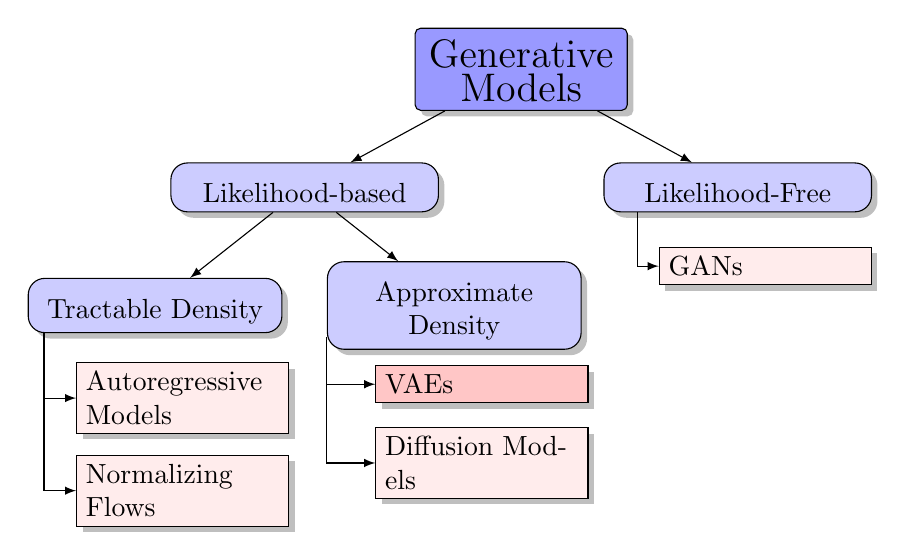
\begin{tikzpicture}[
		basic/.style  = {draw, text width=2cm, drop shadow, rectangle},
		root/.style   = {basic, rounded corners=2pt, thin, text height=1.1em, text width=7em, align=center, fill=blue!40},
		level 1/.style={sibling distance=55mm},
		level 2/.style = {basic, rounded corners=6pt, thin, align=center, fill=blue!20, text height=1.1em, text width=9em, sibling distance=38mm},
		level 3/.style = {basic, rounded corners=6pt, thin,align=center, fill=blue!20, text width=8.5em},
		level 4/.style = {basic, thin, align=left, fill=pink!30, text width=7em},
		level 5/.style = {basic, thin, align=left, fill=pink!90, text width=7em},
		edge from parent/.style={->,draw},
		>=latex]
		
		% root of the the initial tree, level 1
		\node[root] {\Large Generative Models}
		% The first level, as children of the initial tree
		child {node[level 2] (c1) {Likelihood-based}
			child {node[level 3] (c11) {Tractable Density}}
			child {node[level 3] (c12) {Approximate Density}}
		}
		child {node[level 2] (c2) {Likelihood-Free}};
		
		% The second level, relatively positioned nodes
		\begin{scope}[every node/.style={level 5}]
			\node [below of = c12, xshift=10pt] (c121) {VAEs};
		\end{scope}
		
		% The second level, relatively positioned nodes
		\begin{scope}[every node/.style={level 4}]
			\node [below of = c11, yshift=-5pt, xshift=10pt] (c111) {Autoregressive Models};
			\node [below of = c111, yshift=-5pt] (c112) {Normalizing Flows};
			
			\node [below of = c121] (c122) {Diffusion Models};
			\node [below of = c2, xshift=10pt] (c21) {GANs};
		\end{scope}
		
		% lines from each level 1 node to every one of its "children"
		\foreach \value in {1,2}
		\draw[->] (c11.194) |- (c11\value.west);
		
		\foreach \value in {1,2}
		\draw[->] (c12.194) |- (c12\value.west);
		
		\draw[->] (c2.194) |- (c21.west);
		
	\end{tikzpicture}
\end{frame}
%=======
\begin{frame}{Variational Autoencoder (VAE)}
	\begin{block}{Training}
		\begin{itemize}
			\item Pick a batch of samples \{$\bx_i\}_{i=1}^B$ (here we use Monte Carlo technique).
			\eqpause
			\item Compute the objective for each sample (apply the reparametrization trick):
			\vspace{-0.3cm}
			\[
				\bepsilon^* \sim p(\bepsilon); \quad \bz^* = \bg_{\bphi}(\bx, \bepsilon^*);
			\]
			\[
				\cL_{\bphi, \btheta}(\bx) \approx  \log \pt(\bx | \bz^*) - \KL(q_{\bphi}(\bz| \bx) \| p(\bz)).
			\]
			\eqpause
			\vspace{-0.5cm}
			\item Update parameters via stochastic gradient steps with respect to $\bphi$ and $\btheta$.
		\end{itemize}
	\end{block}
	\eqpause
	\begin{block}{Inference}
		\begin{itemize}
			\item Sample $\bz^*$ from the prior $p(\bz)$ ($\cN(0, \bI)$);
			\eqpause
			\item Generate data from the decoder $\pt(\bx | \bz^*)$.
		\end{itemize}
	\end{block}
	\eqpause
	\textbf{Note:} The encoder $q_{\bphi}(\bz| \bx)$ isn't needed during generation.
\end{frame}
%=======
\begin{frame}{Variational Autoencoder}
	\myfootnote{\href{http://ijdykeman.github.io/ml/2016/12/21/cvae.html}{image credit: http://ijdykeman.github.io/ml/2016/12/21/cvae.html} \\ \href{https://arxiv.org/abs/1906.02691}{Kingma D. P., Welling M., An Introduction to Variational Autoencoders, 2019}}
	\vspace{-0.3cm}
	\[
	 	\cL_{q, \btheta}(\bx) = \bbE_{q} \log \pt(\bx | \bz) - \KL (q_{\bphi}(\bz| \bx) \| p(\bz))
	\]
	\vspace{-0.7cm}
	\begin{minipage}[t]{0.6\columnwidth}
		\begin{figure}[h]
			\centering
			\includegraphics[width=\linewidth]{../lecture3/figs/VAE}
		\end{figure}
	\end{minipage}%
	\begin{minipage}[t]{0.4\columnwidth}
		\begin{figure}[h]
			\centering
			\includegraphics[width=\linewidth]{../lecture3/figs/vae_scheme}
		\end{figure}
	\end{minipage}
	\eqpause
	VAEs are widely used as a preliminary stage of projecting data onto low-dimensional space.
\end{frame}
%=======
\begin{frame}{Variational Autoencoder}
	\myfootnotewithlink{https://arxiv.org/abs/2403.18103}{Chan S., Tutorial on Diffusion Models for Imaging and Vision, 2024}
	\begin{itemize}
		\item The encoder $q_{\bphi}(\bz| \bx) = \NN_{e, \bphi}(\bx)$ outputs $\bmu_{\bphi}(\bx)$ and $\bsigma_{\bphi}(\bx)$.
		\item The decoder $\pt(\bx | \bz) = \NN_{d, \btheta}(\bz)$ outputs parameters of the observed data distribution.
	\end{itemize}
	\begin{figure}[h]
		\centering
		\includegraphics[width=0.7\linewidth]{../lecture3/figs/vae-encoder}
	\end{figure}
	\begin{figure}[h]
		\centering
		\includegraphics[width=0.9\linewidth]{../lecture3/figs/vae-decoder}
	\end{figure}
\end{frame}
%=======
\begin{frame}{VAE vs Normalizing Flows}
	\myfootnotewithlink{https://arxiv.org/abs/2007.02731}{Nielsen D., et al., SurVAE Flows: Surjections to Bridge the Gap Between VAEs and Flows, 2020}
	\begin{table}[]
		\begin{tabular}{l|c|c}
			& \textbf{VAE} & \textbf{NF} \\ \hline
			\textbf{Objective} & ELBO $\cL$ & Forward KL/MLE \\ \hline
			\textbf{Encoder} & \shortstack{stochastic \\ $\bz \sim q_{\bphi}(\bz| \bx)$} &  \shortstack{\\ deterministic \\ $\bz = \bff_{\btheta}(\bx)$ \\ $q_{\btheta}(\bz| \bx) = \delta(\bz - \bff_{\btheta}(\bx))$}  \\ \hline
			\textbf{Decoder} & \shortstack{stochastic \\ $\bx \sim \pt(\bx| \bz)$} & \shortstack{\\ deterministic \\ $\bx = \bg_{\btheta}(\bz)$ \\ $ \pt(\bx | \bz) = \delta(\bx - \bg_{\btheta}(\bz))$} \\ \hline
			\textbf{Parameters}  & $\bphi, \btheta$ & $\btheta \equiv \bphi$\\ 
		\end{tabular}
	\end{table}
	\vspace{-0.3cm}
	\eqpause
	\begin{block}{Theorem}
		MLE for a normalizing flow is equivalent to maximizing the ELBO for a VAE where:
		\vspace{-0.3cm}
		\[
			\pt(\bx | \bz) = \delta (\bx - \bff^{-1}_{\btheta}(\bz)) = \delta (\bx - \bg_{\btheta}(\bz));
		\]
		\vspace{-0.5cm}
		\[
			q_{\btheta}(\bz| \bx) = \delta (\bz - \bff_{\btheta}(\bx)).
		\]
	\end{block}
\end{frame}
%=======
\begin{frame}{Summary}
	\begin{itemize}
		\item LVMs introduce latent representations for observed data, enabling more interpretable models.
		\vfill
		\item LVMs maximize the variational evidence lower bound (ELBO) to obtain maximum likelihood estimates for the parameters.
		\vfill
		\item Parametric posterior distribution $q_{\bphi}(\bz| \bx)$ makes the method scalable.
		\vfill
		\item The reparametrization trick provides unbiased gradients with respect to the variational posterior $q_{\bphi}(\bz| \bx)$.
		\vfill
		\item The VAE model is a latent variable model parameterized by two neural networks: a stochastic encoder $q_{\bphi}(\bz| \bx)$ and a stochastic decoder $\pt(\bx | \bz)$.
		\vfill
		\item Nowadays, the main role of VAEs is to project data into low-dimensional latent space.
	\end{itemize}
\end{frame}

%================================================================================
% LECTURE 4
%================================================================================
\part{Lecture 4}
\createdgmtitle{4}

%--------------------------------------------------------------------------------
\begin{frame}[noframenumbering,plain]
	\titlepage
	\resetonslide
\end{frame}







%=======
\begin{frame}{Outline}
	\tableofcontents[part=4]
\end{frame}
%=======
\section{Discrete VAE Latent Representations}
%=======
\begin{frame}{Discrete VAE Latents}
	\begin{block}{Motivation}
		\begin{itemize}
			\item Previous VAE models have used \textbf{continuous} latent variables $\bz$.
			\item For some modalities, \textbf{discrete} representations $\bz$ may be a more natural choice.
			\item Advanced autoregressive models (e.g., PixelCNN) are highly effective for distributions over discrete variables.
			\item Current transformer-like models process discrete tokens.
		\end{itemize}
	\end{block}
	\eqpause
	\begin{block}{ELBO}
		\vspace{-0.3cm}
		\[
			\cL_{\bphi, \btheta}(\bx)  = \bbE_{q_{\bphi}(\bz| \bx)} \log \pt(\bx| \bz) - \KL(q_{\bphi}(\bz| \bx) \| p(\bz)) \rightarrow \max_{\bphi, \btheta}.
		\]
		\vspace{-0.5cm}
	\end{block}
	\eqpause
	\begin{itemize}
		\item Apply the reparametrization trick to obtain unbiased gradients.
		\item Use Gaussian distributions for $q_{\bphi}(\bz| \bx)$ and $p(\bz)$ to compute the KL analytically.
	\end{itemize}
\end{frame}
%=======
\begin{frame}{Discrete VAE Latents}
	\begin{block}{Assumptions}
		\begin{itemize}
			\item Let $c \sim \Cat(\bpi)$, where 
			\vspace{-0.6cm}
			\[
			\bpi = (\pi_1, \dots, \pi_K), \quad \pi_k = P(c = k), \quad \sum_{k=1}^K \pi_k = 1.
			\]
			\vspace{-0.6cm}
			\item Suppose the VAE adopts a discrete latent variable $c$ with prior $p(c) = \Uniform\{1, \dots, K\}$.
		\end{itemize}
	\end{block}
	\eqpause
	\begin{block}{ELBO}
		\vspace{-0.5cm}
		\[
			\cL_{\bphi, \btheta}(\bx)  = \bbE_{q_{\bphi}(c| \bx)} \log \pt(\bx| c) - {\color{olive} \KL(q_{\bphi}(c| \bx) \| p(c))} \rightarrow \max_{\bphi, \btheta}.
		\]
	\end{block}
	\vspace{-1.0cm}
	{\small
	\begin{multline*}
		{\color{olive} \KL(q_{\bphi}(c| \bx) \| p(c))} = \sum_{k=1}^K q_{\bphi}(k| \bx) \log \frac{q_{\bphi}(k| \bx)}{p(k)} 
		\nextonslide{= \\ = \color{violet}{\sum_{k=1}^K q_{\bphi}(k| \bx) \log q_{\bphi}(k| \bx)}  \color{teal}{- \sum_{k=1}^K q_{\bphi}(k| \bx) \log p(k)}}
		\nextonslide{= \\ = \color{violet}{- \Ent(q_{\bphi}(c| \bx))} + \color{teal}{\log K}. }
	\end{multline*}
	}
\end{frame}
%=======
\begin{frame}{Discrete VAE Latents}
	\myfootnotewithlink{https://arxiv.org/abs/2403.18103}{Chan S., Tutorial on Diffusion Models for Imaging and Vision, 2024}
	\[
		\cL_{\bphi, \btheta}(\bx)  = \bbE_{q_{\bphi}(c| \bx)} \log \pt(\bx| c) + \Ent(q_{\bphi}(c| \bx)) - \log K \rightarrow \max_{\bphi, \btheta}.
	\]
	\eqpause
	\vspace{-0.5cm}
	\begin{itemize}
		\item The encoder should output a discrete distribution $q_{\bphi}(c| \bx)$.
					\item We need an analogue of the reparametrization trick for discrete $q_{\bphi}(c| \bx)$.
		\item The decoder $\pt(\bx| c)$ must take a discrete random variable $c$ as input.
	\end{itemize}
	\begin{figure}[h]
		\centering
		\includegraphics[width=0.7\linewidth]{../lecture4/figs/vae-encoder}
	\end{figure}
	\begin{figure}[h]
		\centering
		\includegraphics[width=0.9\linewidth]{../lecture4/figs/vae-decoder}
	\end{figure}
\end{frame}
%=======
\section{Vector Quantized VAE}
%=======
\begin{frame}{Vector Quantization}
	\myfootnotewithlink{https://arxiv.org/abs/2004.02088}{Zhao Y. et al. Feature Quantization Improves GAN Training, 2020} 
	Define the codebook (dictionary) space $\{\be_k\}_{k=1}^K$ with $\be_k \in \bbR^L$ and $K$ the number of codebook entries.
    \eqpause
	\begin{block}{Quantized Representation}
		A quantized vector $\bz_q \in \bbR^{L}$, for any $\bz \in \bbR^L$, is defined via nearest-neighbor lookup in the codebook:
		\vspace{-0.3cm}
		\[
			\bz_q = \bq (\bz) = \be_{k^*}, \quad \text{where } k^* = \argmin_k \| \bz - \be_k \|.
		\] 
		\vspace{-0.7cm}
	\end{block}
	\eqpause
	\vspace{-0.2cm}
	\begin{block}{Quantization Procedure}
		If the encoded tensor has spatial dimensions, quantization is independently applied to each of the $W \times H$ locations.
		\begin{minipage}[t]{0.65\columnwidth}
			\begin{figure}
				\includegraphics[width=0.8\linewidth]{../lecture4/figs/fqgan_cnn.png}
			\end{figure}
		\end{minipage}%
		\begin{minipage}[t]{0.35\columnwidth}
			\begin{figure}
				\includegraphics[width=0.7\linewidth]{../lecture4/figs/fqgan_lookup}
			\end{figure}
		\end{minipage}
	\end{block}
\end{frame}
%=======
\begin{frame}{Vector Quantized VAE (VQ-VAE)}
	\myfootnotewithlink{https://arxiv.org/abs/1711.00937}{Oord A., Vinyals O., Kavukcuoglu K. Neural Discrete Representation Learning, 2017} 
	\begin{itemize}
		\item The encoder outputs a continuous vector $\bz_e = \NN_{e, \bphi}(\bx) \in \bbR^{L}$.
		\item Quantization deterministically maps $\bz_e$ to its quantized codebook vector $\bz_q$.
		\item The decoder is conditioned on codebook entries $\be_c$, i.e., via $\pt(\bx | \be_c)$ (instead of $\pt(\bx| c)$).
	\end{itemize}
    \eqpause
	\begin{block}{Deterministic Variational Posterior}
		\vspace{-0.3cm}
		\[
			q_{\bphi}(c = k^* | \bx) = \begin{cases}
				1 , \quad \text{for } k^* = \argmin_k \| \bz_e - \be_k \|; \\
				0, \quad \text{otherwise}.
		\end{cases}
		\]
        \eqpause
		\[
			\KL(q_{\bphi}(c| \bx) \| p(c)) = - \underbrace{\Ent(q_{\bphi}(c| \bx))}_{=0} + \log K = \log K. 
		\]
        \eqpause
	\end{block}	
	\vspace{-0.4cm}
	\textbf{Note:} The KL regularizer becomes constant and has no direct effect on the ELBO objective in this case.
\end{frame}
%=======
\begin{frame}{Vector Quantized VAE (VQ-VAE): Forward}
	\myfootnotewithlink{https://arxiv.org/abs/1711.00937}{Oord A., Vinyals O., Kavukcuoglu K. Neural Discrete Representation Learning, 2017} 
	\begin{block}{Deterministic Variational Posterior}
		\vspace{-0.3cm}
		\[
			q_{\bphi}(c = k^* | \bx) = \begin{cases}
			1 , \quad \text{if } k^* = \argmin_k \| \bz_e - \be_k \|; \\
			0, \quad \text{otherwise}.
			\end{cases}
		\]
	\vspace{-0.5cm}
	\end{block}	
    \eqpause
	\begin{block}{ELBO}
		\vspace{-0.6cm}
		\[
			\cL_{\bphi, \btheta}(\bx)  = \bbE_{q_{\bphi}(c| \bx)} \log \pt(\bx| \be_{c}) - \log K \nextonslide{= \log \pt(\bx| \bz_q) - \log K,}
		\]
		where $\bz_q = \be_{k^*}$, $k^* = \argmin_k \| \bz_e - \be_k \|$.
	\end{block}
    \eqpause
	\vspace{-0.3cm} 
	\begin{figure}
		\centering
		\includegraphics[width=0.85\linewidth]{../lecture4/figs/vqvae}
	\end{figure}
    \eqpause
	\vspace{-0.3cm} 
	\textbf{Challenge:} The $\argmin$ operation is non-differentiable.
\end{frame}
%=======
\begin{frame}{Vector Quantized VAE (VQ-VAE): Backward}
	\myfootnotewithlink{https://arxiv.org/abs/1711.00937}{Oord A., Vinyals O., Kavukcuoglu K. Neural Discrete Representation Learning, 2017} 
	\begin{block}{ELBO}
		\vspace{-0.5cm}
		\[
			\cL_{\bphi, \btheta}(\bx)  =  \log \pt(\bx| \bz_q) - \log K, \quad \bz_q = \be_{k^*},\; k^* = \argmin_k \| \bz_e - \be_k \|.
		\]
		\vspace{-0.5cm}
	\end{block}
    \eqpause
	\begin{figure}
		\centering
		\includegraphics[width=0.85\linewidth]{../lecture4/figs/vqvae}
	\end{figure}
    \eqpause
	\vspace{-0.3cm}
	\begin{block}{Straight-Through Gradient Estimator}
		\vspace{-0.5cm}
		\begin{multline*}
		\frac{\partial \log p(\bx | \bz_q , \btheta)}{\partial \bphi} = \frac{\partial \log \pt(\bx| \bz_q)}{\partial \bz_q} \cdot {\color{red}\frac{\partial \bz_q}{\partial \bphi}} = \\
		\nextonslide{= \frac{\partial \log \pt(\bx| \bz_q)}{\partial \bz_q} \cdot {\color{red}\frac{\partial \bz_q}{\partial \bz_e}} \cdot \frac{\partial \bz_e}{\partial \bphi}}
		\nextonslide{\approx \frac{\partial \log \pt(\bx| \bz_q)}{\partial \bz_q} \cdot \frac{\partial \bz_e}{\partial \bphi}}
		\end{multline*}
	\end{block}
\end{frame}
%=======
\begin{frame}{Vector Quantized VAE-2 (VQ-VAE-2)}
	\myfootnotewithlink{https://arxiv.org/abs/1906.00446}{Razavi A., Oord A., Vinyals O. Generating Diverse High-Fidelity Images with VQ-VAE-2, 2019} 
	Extension to the spatial domain: $\bc \in \{1, \dots, K\}^{W \times H}$
	\vspace{-0.3cm}
	\[
		q_{\bphi}(\bc | \bx) = \prod_{i=1}^W \prod_{j=1}^H q(c_{ij} | \bx, \bphi); \quad p(\bc) = \prod_{i=1}^W \prod_{j=1}^H \Uniform\{1, \dots, K\}.
	\]
	\vspace{-0.6cm}
	\begin{block}{Sample Diversity}
		\vspace{-0.2cm}
		\begin{figure}
			\centering
			\includegraphics[width=1.0\linewidth]{../lecture4/figs/vqvae2_diversity}
		\end{figure}
	\end{block}
\end{frame}
%=======
\begin{frame}{Vector Quantized VAE (VQ-VAE): Final algorithm}
	\begin{block}{Training}
		\begin{itemize}
			\item Vector-quantize (per spatial location if applicable):
			\vspace{-0.3cm}
			\[
				k^* = \argmin_k \|\bz_e - \be_k\|_2, \quad \bz_q = \be_{k^*}, \quad \bz_e = \NN_{e,\bphi}(\bx).
			\]
			\vspace{-0.5cm}
			\item Compute ELBO objective:
			\vspace{-0.3cm}
			\[
				\cL_{\bphi, \btheta}(\bx) = \log \pt(\bx | \bz_q) - \log K.
			\]
			\vspace{-0.5cm}
			\item Compute total loss with codebook and commitment losses (with stop-gradient $\text{sg}[\cdot]$):
			\vspace{-0.3cm}
			\[
				\cL = - \cL_{\bphi, \btheta}(\bx) + \big\|\text{sg}[\bz_e] - \be_{k^*}\big\|_2^2 + \beta \big\|\bz_e - \text{sg}[\be_{k^*}]\big\|_2^2
			\]
			\vspace{-0.5cm}
			\item Use straight-through gradient estimation for encoder.
		\end{itemize}
	\end{block}
	\eqpause
	\vspace{-0.3cm}
	\begin{block}{Sampling}
		\begin{itemize}
			\item Sample $c \sim p(c) = \Uniform\{1, \dots, K\}$.
			\item Generate $\bx \sim \pt(\bx | \be_c)$.
		\end{itemize}
	\end{block}
\end{frame}
%=======
\section{ELBO Surgery}
%=======
\begin{frame}{ELBO Surgery}
	\myfootnotewithlink{http://approximateinference.org/accepted/HoffmanJohnson2016.pdf}{Hoffman M. D., Johnson M. J. ELBO Surgery: Yet Another Way to Carve Up the Variational Evidence Lower Bound, 2016}
	\vspace{-0.3cm}
	\[
	    \frac{1}{n} \sum_{i=1}^n \cL_{\bphi, \btheta}(\bx_i) = \frac{1}{n} \sum_{i=1}^n \Bigl[ \bbE_{q_{\bphi}(\bz| \bx_i)} \log \pt(\bx_i | \bz) - \KL(q_{\bphi}(\bz| \bx_i) \| p(\bz)) \Bigr].
	\]
    \eqpause
	\vspace{-0.3cm}
	\begin{block}{Theorem}
		\vspace{-0.5cm}
		\[
		    \frac{1}{n} \sum_{i=1}^n \KL(q_{\bphi}(\bz| \bx_i) \| p(\bz)) = {\color{violet} \KL(q_{\text{agg}, \bphi}(\bz) \| p(\bz))} + {\color{teal}\bbI_{q} [\bx, \bz]};
		\]
        \eqpause
		\vspace{-0.5cm}
		\begin{itemize}
			\item $q_{\text{agg}, \bphi}(\bz) = \frac{1}{n} \sum_{i=1}^n q_{\bphi}(\bz| \bx_i)$ denotes the \textbf{aggregated} variational posterior.
			\item $\bbI_{q} [\bx, \bz]$ is the mutual information between $\bx$ and $\bz$ under the data distribution $\pd(\bx)$ and $q_{\bphi}(\bz| \bx)$.
			\item  {\color{violet} The first term} encourages $q_{\text{agg}, \bphi}(\bz)$ to match the prior $p(\bz)$.
			\item {\color{teal} The second term} reduces the information about $\bx$ encoded in~$\bz$.
		\end{itemize}
	\end{block}
\end{frame}
%=======
\begin{frame}{ELBO Surgery}
	\myfootnotewithlink{http://approximateinference.org/accepted/HoffmanJohnson2016.pdf}{Hoffman M. D., Johnson M. J. ELBO Surgery: Yet Another Way to Carve Up the Variational Evidence Lower Bound, 2016}
		\vspace{-0.4cm}
		\[
		    \frac{1}{n} \sum_{i=1}^n \KL(q_{\bphi}(\bz| \bx_i) \| p(\bz)) = \KL(q_{\text{agg}, \bphi}(\bz) \| p(\bz)) + \bbI_q [\bx, \bz].
		\]
		\vspace{-0.3cm}
	\begin{block}{Proof}
		\vspace{-0.5cm}
		{\footnotesize
		\begin{multline*}
		    \frac{1}{n} \sum_{i=1}^n \KL(q_{\bphi}(\bz| \bx_i) \| p(\bz)) = \frac{1}{n} \sum_{i=1}^n \int q_{\bphi}(\bz| \bx_i) \log \frac{q_{\bphi}(\bz| \bx_i)}{p(\bz)} d \bz
		    \nextonslide{= \\= \frac{1}{n} \sum_{i=1}^n \int q_{\bphi}(\bz| \bx_i) \log \frac{{\color{violet}q_{\text{agg}, \bphi}(\bz)} {\color{teal}q_{\bphi}(\bz| \bx_i)}}{{\color{violet}p(\bz)} {\color{teal}q_{\text{agg}, \bphi}(\bz)}} d \bz}
		    \nextonslide{= \\ = \int \frac{1}{n} \sum_{i=1}^n  q_{\bphi}(\bz| \bx_i) \log {\color{violet}\frac{q_{\text{agg}, \bphi}(\bz)}{p(\bz)}} d \bz + \frac{1}{n}\sum_{i=1}^n \int q_{\bphi}(\bz| \bx_i) \log {\color{teal}\frac{q_{\bphi}(\bz| \bx_i)}{q_{\text{agg}, \bphi}(\bz)}} d \bz}
		    \nextonslide{= \\ = \KL (q_{\text{agg}, \bphi}(\bz) \| p(\bz)) + \frac{1}{n}\sum_{i=1}^n \KL(q_{\bphi}(\bz| \bx_i) \| q_{\text{agg}, \bphi}(\bz))}
		\end{multline*}
        \eqpause
		}
		\vspace{-0.4cm}
		\[
			\bbI_{q} [\bx, \bz] = \frac{1}{n}\sum_{i=1}^n \KL(q_{\bphi}(\bz| \bx_i) \| q_{\text{agg}, \bphi}(\bz)).
		\]
	\end{block}
\end{frame}
%=======
\begin{frame}{ELBO Surgery}
	\myfootnotewithlink{http://approximateinference.org/accepted/HoffmanJohnson2016.pdf}{Hoffman M. D., Johnson M. J. ELBO Surgery: Yet Another Way to Carve Up the Variational Evidence Lower Bound, 2016}
	\vspace{-0.3cm}
	\begin{block}{Revisiting the ELBO}
		\vspace{-0.7cm}
		{\small
		\begin{multline*}
		    \frac{1}{n}\sum_{i=1}^n \cL_{\bphi, \btheta}(\bx_i) = \frac{1}{n} \sum_{i=1}^n \left[ \bbE_{q_{\bphi}(\bz| \bx_i)} \log \pt(\bx_i | \bz) - \KL(q_{\bphi}(\bz| \bx_i) \| p(\bz)) \right]
		    \nextonslide{= \\ = \underbrace{\frac{1}{n} \sum_{i=1}^n \bbE_{q_{\bphi}(\bz| \bx_i)} \log \pt(\bx_i | \bz)}_{\text{Reconstruction Loss}} - \underbrace{\vphantom{ \sum_{i=1}^n} \bbI_q [\bx, \bz]}_{\text{Mutual Information}} - \underbrace{\vphantom{ \sum_{i=1}^n} \KL(q_{\text{agg}, \bphi}(\bz) \| {\color{teal}p(\bz)})}_{\text{Marginal KL}}}
		\end{multline*}
		}
		\vspace{-0.3cm}
	\end{block}
    \eqpause
	The prior distribution $p(\bz)$ only appears in the last term.
    \eqpause
	\begin{block}{Optimal VAE Prior}
		\vspace{-0.7cm}
		\[
	  		\KL(q_{\text{agg}, \bphi}(\bz) \| p(\bz)) = 0 \quad \Leftrightarrow \quad p (\bz) = q_{\text{agg}, \bphi}(\bz) = \frac{1}{n} \sum_{i=1}^n q_{\bphi}(\bz| \bx_i).
		\]
        \eqpause
		\vspace{-0.4cm} \\
		Hence, the optimal prior $p(\bz)$ is the aggregated variational posterior $q_{\text{agg}, \bphi}(\bz)$.
	\end{block}
\end{frame}
%=======
\begin{frame}{Marginal KL}
	\myfootnotewithlink{https://arxiv.org/abs/1505.05770}{Rezende D. J., Mohamed S. Variational Inference with Normalizing Flows, 2015} 
	\[
		\KL(q_{\text{agg}, \bphi}(\bz) \| p(\bz))
	\]
	\vspace{-0.5cm}
	\begin{itemize}
		\item $q_{\bphi}(\bz| \bx) = \cN(\bmu_{\bphi}(\bx), \bsigma^2_{\bphi}(\bx))$ is unimodal. 
		\item It is generally believed that the \textbf{mismatch between} $p(\bz)$  \textbf{and} $q_{\text{agg}, \bphi}(\bz)$  is the primary explanation for blurry VAE-generated images.
	\end{itemize}
    \eqpause
	\begin{figure}
		\includegraphics[width=0.8\linewidth]{../lecture4/figs/agg_posterior}
	\end{figure}
\end{frame}
%=======
\section{Learnable VAE Prior}
%=======
\begin{frame}{Optimal VAE Prior}
	\myfootnotewithlink{https://jmtomczak.github.io/blog/7/7\_priors.html}{image credit: https://jmtomczak.github.io/blog/7/7\_priors.html}
	\begin{itemize}
		\item Standard Gaussian $p(\bz) = \cN(0, \bI)$ often leads to over-regularization.
		\item $p(\bz) = q_{\text{agg}, \bphi}(\bz) = \frac{1}{n}\sum_{i=1}^n q_{\bphi}(\bz| \bx_i)$ risks overfitting and incurs high computational cost.
	\end{itemize}
    \eqpause
	\vspace{-0.5cm}
	\begin{minipage}[t]{0.5\columnwidth}
		\begin{block}{Non-Learnable Prior $p(\bz)$}
			\begin{figure}[h]
				\centering
				\includegraphics[width=0.6\linewidth]{../lecture4/figs/non_learnable_prior}
			\end{figure}
		\end{block}
	\end{minipage}%
	\begin{minipage}[t]{0.5\columnwidth}
		\begin{block}{Learnable Prior $p_{\blambda}(\bz)$}
			\begin{figure}[h]
				\centering
				\includegraphics[width=0.6\linewidth]{../lecture4/figs/learnable_prior}
			\end{figure}
		\end{block}
	\end{minipage}
    \eqpause
	\vspace{-0.3cm}
	\[
	\frac{1}{n}\sum_{i=1}^n \cL_{\bphi, \btheta}(\bx_i) = \text{RL} - \text{MI} -  \KL(q_{\text{agg}, \bphi}(\bz) \| {\color{teal}p_{\blambda}(\bz)})
	\]
	This is the forward KL divergence with respect to $p_{\blambda}(\bz)$.
\end{frame}
%=======
\begin{frame}{NF-Based VAE Prior}
	\myfootnotewithlink{https://arxiv.org/abs/1611.02731}{Chen X. et al. Variational Lossy Autoencoder, 2016}
	\begin{block}{NF Model in Latent Space}
		\vspace{-0.5cm}
		\[
			\log p_{\blambda}(\bz) = \log p(\bz^*) + \log  \left | \det \left(\frac{d \bz^*}{d\bz}\right)\right| = \log p(\bff_{\blambda}(\bz)) + \log \left | \det (\bJ_\bff)\right| 
		\]
		\vspace{-0.3cm}
		\[
			\bz = \bg_{\blambda}(\bz^*) = \bff^{-1}_{\blambda}(\bz^*)
		\]
	\end{block}
    \eqpause
	\vspace{-0.3cm}
	\begin{itemize}
		\item RealNVP with coupling layers,
		\item Autoregressive normalizing flows (efficient $\bff_{\blambda}(\bz)$, but $\bg_{\blambda}(\bz^*)$ can be slow).
	\end{itemize}
    \eqpause
	\begin{block}{ELBO with NF-Based VAE Prior}
		\vspace{-0.5cm}
		{\small
			\begin{multline*}
				\cL_{\bphi, \btheta}(\bx) = \bbE_{q_{\bphi}(\bz| \bx)} \log \pt(\bx| \bz) - \KL(q_{\bphi}(\bz| \bx) \| p(\bz))
				\nextonslide{= \\ = \bbE_{q_{\bphi}(\bz| \bx)} \left[ \log \pt(\bx | \bz) + {\color{violet}\log p_{\blambda}(\bz)} - \log q_{\bphi}(\bz| \bx) \right]}
				\nextonslide{= \\ = \bbE_{q_{\bphi}(\bz| \bx)} \Bigl[ \log \pt(\bx | \bz) + \underbrace{ \Bigl({\color{violet} \log p(\bff_{\blambda}(\bz)) + \log \left| \det (\bJ_\bff) \right|} \Bigr) }_{\text{NF-based prior}} - \log q_{\bphi}(\bz| \bx) \Bigr]} 
			\end{multline*}
		}
	\end{block}
\end{frame}
%=======
\begin{frame}{Summary}
	\begin{itemize}
		\item Discrete VAE latents offer a natural class of latent variable models.	
		\vfill
		\item Vector quantization provides a way to construct VAEs with discrete latents and deterministic variational posteriors.
		\vfill
		\item The straight-through gradient estimator allows gradients to pass as if quantization were an identity operation during backpropagation.			
		\vfill
		\item ELBO surgery gives insights into the prior's influence in VAEs; the optimal prior is the aggregated variational posterior. 
		\vfill
		\item The mismatch between $p(\bz)$ and $q_{\text{agg}, \bphi}(\bz)$ is widely regarded as the principal reason for VAE-generated image blurriness.
		\vfill
		\item Normalizing flow-based priors, including autoregressive flows, can be incorporated directly into VAEs.	
	\end{itemize}
\end{frame}
%=======

%================================================================================
% LECTURE 5
%================================================================================
\part{Lecture 5}
\createdgmtitle{5}

%--------------------------------------------------------------------------------
\begin{frame}[noframenumbering,plain]
	\titlepage
	\resetonslide
\end{frame}




%=======
\begin{frame}{Outline}
	\tableofcontents[part=5]
\end{frame}
%=======
\begin{frame}{Outline}
	\tableofcontents[part=5]
\end{frame}
%=======
\section{Likelihood-Free Learning}
%=======
\begin{frame}{Likelihood-Based Models}
	\myfootnotewithlink{https://arxiv.org/abs/1511.01844}{Theis L., Oord A., Bethge M. A Note on the Evaluation of Generative Models, 2015}
	\begin{minipage}[t]{0.48\columnwidth}
		\vspace{-0.3cm}
		\begin{block}{Poor Likelihood \\ High-Quality Samples}
			\vspace{-0.3cm}
			\[
				p_1(\bx) = \frac{1}{n} \sum_{i=1}^n \cN(\bx | \bx_i, \epsilon \bI)
			\]
			If $\epsilon$ is very small, this model produces excellent, sharp samples but achieves poor likelihoods on test data.
		\end{block}	
	\end{minipage}%
	\begin{minipage}[t]{0.52\columnwidth}
		\eqpause
		\vspace{-0.3cm}
		\begin{block}{High Likelihood \\ Poor Samples}
			\vspace{-0.5cm}
			\[
				p_2(\bx) = 0.01p(\bx) + 0.99p_{\text{noise}}(\bx)
			\]
			\vspace{-1.0cm}
			\begin{multline*}
				\log \left[ 0.01p(\bx) + 0.99p_{\text{noise}}(\bx) \right] \geq \\ \geq \log \left[ 0.01p(\bx) \right]  = \log p(\bx) - \log 100
			\end{multline*}
			This model contains mostly noisy, irrelevant samples; for high dimensions, $\log p(\bx)$ scales linearly with $m$.
		\end{block}
	\end{minipage}
	\eqpause
	\begin{itemize}
		\item Likelihood isn't always a suitable metric for evaluating generative models.
		\item Sometimes, the likelihood function can't even be computed exactly.
	\end{itemize}
\end{frame}
%=======
\begin{frame}{Likelihood-Free Learning}
	\begin{block}{Motivation}
	 We're interested in approximating the true data distribution~$\pd(\bx)$.
	Instead of searching over all distributions, let's learn a model $\pt(\bx) \approx \pd(\bx)$.
	\end{block}
	\eqpause
	Suppose we have two sets of samples: 
	\begin{itemize}
		\item $\{\bx_i\}_{i=1}^{n_1} \sim \pd(\bx)$ — real data;
		\item $\{\bx_i\}_{i=1}^{n_2} \sim \pt(\bx)$ — generated (fake) data.
	\end{itemize}
	\eqpause
	Define a discriminative model (classifier):
	\[
		p(y = 1 | \bx) = P(\bx \sim \pd(\bx)); \quad p(y = 0 | \bx) = P(\bx \sim \pt(\bx))
	\]
	\eqpause
	\vspace{-0.5cm}
	\begin{block}{Assumption}
		The generative model $\pt(\bx)$ matches $\pd(\bx)$ if a discriminative model $p(y | \bx)$ can't distinguish between them --- that is, if $p(y = 1 | \bx) = 0.5$ for every $\bx$.
	\end{block}
\end{frame}
%=======
\begin{frame}{Generative Adversarial Networks (GAN)}
	\myfootnotewithlink{https://arxiv.org/abs/1406.2661}{Goodfellow I. J. et al. Generative Adversarial Networks, 2014}
	\begin{itemize}
		\item The more expressive the discriminator, the closer we get to the optimal $\pt(\bx)$.
		\item Standard classifiers are trained by minimizing cross-entropy loss $-\bbE_{\hat{p}(\bx, y)} \log p(y | \bx)$ with $\hat{p}(\bx, y) = \frac{1}{2} [y=1]\pd(\bx) + \frac{1}{2} [y=0]\pt(\bx)$.
	\end{itemize}
	\eqpause
	\begin{block}{Cross-Entropy for Discriminator}
		\vspace{-0.3cm}
		\[
			\min_{p(y | \bx)} \left[ - \bbE_{\pd(\bx)} \log p(y = 1 | \bx) - \bbE_{\pt(\bx)} \log p(y = 0 | \bx) \right] 
		\]
		\[
			\max_{p(y | \bx)} \left[\bbE_{\pd(\bx)} \log p(y = 1 | \bx) + \bbE_{\pt(\bx)} \log p(y = 0 | \bx) \right] 
		\]
	\end{block}
	\eqpause
	\vspace{-0.3cm}
	\begin{block}{Generative Model}
		Suppose $\pt(\bx, \bz) = \pt(\bx| \bz) p(\bz)$, where $p(\bz)$ is a base distribution, and $\pt(\bx | \bz) = \delta (\bx - \bG_{\btheta}(\bz))$ is deterministic.
	\end{block}
\end{frame}
%=======
\begin{frame}{Generative Adversarial Networks (GAN)}
	\myfootnotewithlink{https://arxiv.org/abs/1406.2661}{Goodfellow I. J. et al. Generative Adversarial Networks, 2014}
	\begin{block}{Cross-Entropy for Discriminative Model}
		\vspace{-0.3cm}
		\[
			\max_{p(y | \bx)} \left[\bbE_{\pd(\bx)} \log p(y = 1 | \bx) + \bbE_{\pt(\bx)} \log p(y = 0 | \bx) \right] 
		\]
	\end{block}
	\eqpause
	\begin{itemize}
		\item \textbf{Discriminator:} A classifier $p_{\bphi}(y = 1 | \bx) = D_{\bphi}(\bx) \in [0, 1]$, distinguishing real and generated samples. The discriminator aims to \textbf{maximize} cross-entropy.
		\item \textbf{Generator:} The generative model $\bx = \bG_{\btheta}(\bz),\; \bz \sim p(\bz)$, seeks to fool the discriminator. The generator aims to \textbf{minimize} cross-entropy.
	\end{itemize}
	\eqpause
	\begin{block}{GAN Objective}
		\vspace{-0.5cm}
		\[
			\min_{G} \max_D \left[ \bbE_{\pd(\bx)} \log D(\bx) + \bbE_{\pt(\bx)} \log (1 - D(\bx)) \right] 
		\]
		\eqpause
		\[
			\min_{G} \max_D \left[ \bbE_{\pd(\bx)} \log D(\bx) + \bbE_{p(\bz)} \log (1 - D(\bG(\bz))) \right]
		\]
	\end{block}
\end{frame}
%=======
\section{Generative Adversarial Networks (GAN)}
%=======
\begin{frame}{Generative Models Zoo}
	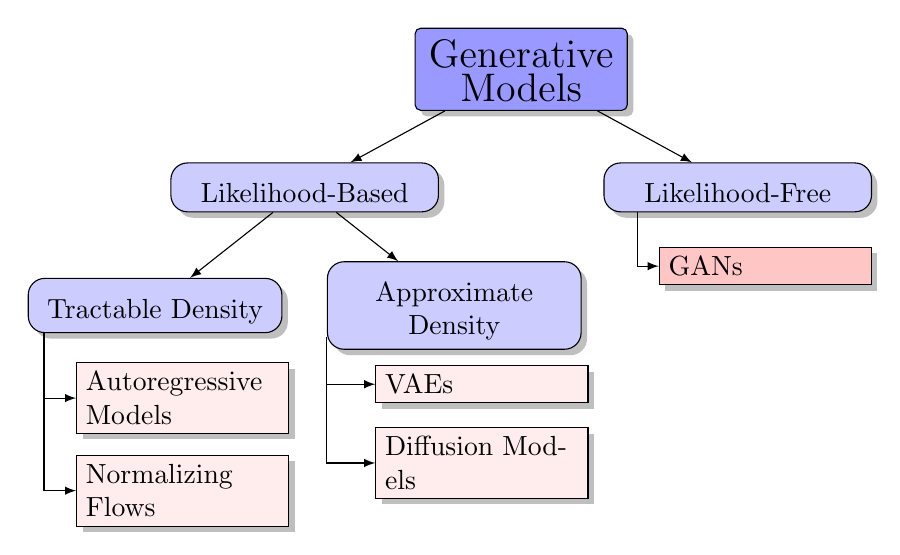
\begin{tikzpicture}[
	 	basic/.style  = {draw, text width=2cm, drop shadow, rectangle},
	 	root/.style   = {basic, rounded corners=2pt, thin, text height=1.1em, text width=7em, align=center, fill=blue!40},
	 	level 1/.style={sibling distance=55mm},
	 	level 2/.style = {basic, rounded corners=6pt, thin, align=center, fill=blue!20, text height=1.1em, text width=9em, sibling distance=38mm},
	 	level 3/.style = {basic, rounded corners=6pt, thin,align=center, fill=blue!20, text width=8.5em},
	 	level 4/.style = {basic, thin, align=left, fill=pink!30, text width=7em},
	 	level 5/.style = {basic, thin, align=left, fill=pink!90, text width=7em},
		edge from parent/.style={->,draw},
		>=latex]
		
		\node[root] {\Large Generative Models}
		child {node[level 2] (c1) {Likelihood-Based}
			child {node[level 3] (c11) {Tractable Density}}
			child {node[level 3] (c12) {Approximate Density}}
		}
		child {node[level 2] (c2) {Likelihood-Free}};
		
		\begin{scope}[every node/.style={level 4}]
		\node [below of = c11, yshift=-5pt, xshift=10pt] (c111) {Autoregressive Models};
		\node [below of = c111, yshift=-5pt] (c112) {Normalizing Flows};
		
		\node [below of = c12, xshift=10pt] (c121) {VAEs};
		\node [below of = c121] (c122) {Diffusion Models};
		\end{scope}
		
		\begin{scope}[every node/.style={level 5}]
		\node [below of = c2, xshift=10pt] (c21) {GANs};
		\end{scope}
		
		\foreach \value in {1,2}
		\draw[->] (c11.194) |- (c11\value.west);
		
		\foreach \value in {1,2}
		\draw[->] (c12.194) |- (c12\value.west);
		
		\draw[->] (c2.194) |- (c21.west);
		
	\end{tikzpicture}
\end{frame}
%=======
\begin{frame}{GAN Optimality}
	\myfootnotewithlink{https://arxiv.org/abs/1406.2661}{Goodfellow I. J. et al. Generative Adversarial Networks, 2014}
	\begin{block}{Theorem}
		The minimax game
		\vspace{-0.3cm}
		\[
			\min_{G} \max_D \Bigl[ \underbrace{\bbE_{\pd(\bx)} \log D(\bx) + \bbE_{p(\bz)} \log (1 - D(\bG(\bz)))}_{V(G, D)} \Bigr]
		\]
		\vspace{-0.5cm} \\
		achieves its global optimum when $\pd(\bx) = \pt(\bx)$, and $D^*(\bx) = 0.5$.
	\end{block}
	\eqpause
	\begin{block}{Proof (Fixed $G$)}
		\vspace{-0.5cm}
		\begin{align*}
			V(G, D) &= \bbE_{\pd(\bx)} \log D(\bx) + \bbE_{\pt(\bx)} \log (1 - D(\bx)) \\
			\nextonslide{&= \int \underbrace{\left[ \pd(\bx) \log D(\bx) + \pt(\bx)\log (1 - D(\bx)) \right]}_{y(D)} d \bx}
		\end{align*}
		\eqpause
		\vspace{-0.2cm}
		\[
			\frac{d y(D)}{d D} = \frac{\pd(\bx)}{D(\bx)} - \frac{\pt(\bx)}{1 - D(\bx)} = 0 \qquad \Rightarrow \quad D^*(\bx) = \frac{\pd(\bx)}{\pd(\bx) + \pt(\bx)}
		\]
	\end{block}
\end{frame}
%=======
\begin{frame}{GAN Optimality}
	\myfootnotewithlink{https://arxiv.org/abs/1406.2661}{Goodfellow I. J. et al. Generative Adversarial Networks, 2014}
	\begin{block}{Proof Continued (Fixed $D = D^*$)}
		\vspace{-0.5cm}
		{\small
		\begin{multline*}
			V(G, D^*) = \bbE_{\pd(\bx)} \log \left( \frac{\pd(\bx)}{\pd(\bx) + \pt(\bx)} \right) + \bbE_{\pt(\bx)} \log \left( \frac{\pt(\bx)}{\pd(\bx) + \pt(\bx)}\right)  \\
		 \nextonslide{= \KL \left(\pd(\bx) \,\|\, \frac{\pd(\bx) + \pt(\bx)}{2}\right) + \KL \left(\pt(\bx) \,\|\, \frac{\pd(\bx) + \pt(\bx)}{2}\right) - 2\log 2 \\}
		 \nextonslide{= 2\,\JSD(\pd(\bx) \,\|\, \pt(\bx)) - 2\log 2.}
		\end{multline*}
		}
	\end{block}
	\eqpause
	\vspace{-0.3cm}
	\begin{block}{Jensen-Shannon Divergence (Symmetric KL Divergence)}
		\vspace{-0.3cm}
		\[
			\JSD(\pd(\bx) \| \pt(\bx)) = \frac{1}{2} \left[\KL \left(\pd(\bx) \| {\color{teal}\star}\right) + \KL \left(\pt(\bx) \| {\color{teal}\star}\right) \right]
		\]
	\end{block}
	\eqpause
	This can be regarded as a proper distance metric!
	\[
		V(G^*, D^*) = -2\log 2, \quad \pd(\bx) = \pt(\bx), \quad  D^*(\bx) = 0.5.
	\]
\end{frame}
%=======
\begin{frame}{GAN Optimality}
	\myfootnotewithlink{https://arxiv.org/abs/1406.2661}{Goodfellow I. J. et al. Generative Adversarial Networks, 2014}
	\begin{block}{Theorem}
		The following minimax game 
		\vspace{-0.3cm}
		\[
		\min_{G} \max_D \Bigl[ \bbE_{\pd(\bx)} \log D(\bx) + \bbE_{p(\bz)} \log (1 - D(\bG(\bz))) \Bigr]
		\]
		\vspace{-0.5cm} \\
		achieves its global optimum precisely when $\pd(\bx) = \pt(\bx)$, and $D^*(\bx) = 0.5$.
	\end{block}
	\vspace{-0.2cm}
	\begin{block}{Expectations}
		If the generator can express \textbf{any} function and the discriminator is \textbf{optimal} at every step, the generator \textbf{will converge} to the target distribution.
	\end{block}
	\vspace{-0.3cm}
	\eqpause
	\begin{block}{Reality}
		\begin{itemize}
			\item Generator updates are performed in parameter space, and the discriminator is often imperfectly optimized.
			\item Generator and discriminator losses typically oscillate during GAN training.
		\end{itemize}
	\end{block}
\end{frame}
%=======
\begin{frame}{GAN Training}
	\myfootnotewithlink{https://arxiv.org/abs/1406.2661}{Goodfellow I. J. et al. Generative Adversarial Networks, 2014}

	Assume both generator and discriminator are parametric models: $D_{\bphi}(\bx)$ and $\bG_{\btheta}(\bz)$.
	\begin{block}{Objective}
		\vspace{-0.7cm}
		\[
		\min_{\btheta} \max_{\bphi} \left[ \bbE_{\pd(\bx)} \log D_{\bphi}(\bx) + \bbE_{p(\bz)} \log (1 - D_{\bphi}(\bG_{\btheta}(\bz))) \right]
		\]
		\vspace{-0.7cm}
	\end{block}
	\eqpause
	\begin{figure}
		\centering
		\includegraphics[width=1.0\linewidth]{../lecture5/figs/gan_1}
	\end{figure}
	\vspace{-0.5cm}
	\eqpause
	\begin{itemize}
		\item $\bz \sim p(\bz)$ is a latent variable.
		\item $\pt(\bx | \bz) = \delta(\bx - \bG_{\btheta}(\bz))$ serves as a deterministic decoder ({\color{gray}like normalizing flows}).
		\item There is no encoder present.
	\end{itemize}
\end{frame}
%=======
\begin{frame}{Mode Collapse}
	\myfootnote{\href{https://arxiv.org/abs/1406.2661}{Goodfellow I. J. et al. Generative Adversarial Networks, 2014} \\
		\href{https://arxiv.org/abs/1611.02163}{Metz L. et al. Unrolled Generative Adversarial Networks, 2016}}
	Mode collapse refers to the phenomenon where the generator in a GAN produces only one or a few different modes of the distribution.
	\vspace{-0.1cm}
	\begin{figure}
		\centering
		\includegraphics[width=0.75\linewidth]{../lecture5/figs/mode_collapse_1}
	\end{figure}
	\vspace{-0.3cm}
	\begin{figure}
		\centering
		\includegraphics[width=1.0\linewidth]{../lecture5/figs/mode_collapse_4}
	\end{figure}
	\eqpause
	Numerous methods have been proposed to tackle mode collapse: changing architectures, adding regularization terms, injecting noise.
\end{frame}
%=======
\begin{frame}{Jensen-Shannon vs Kullback-Leibler Divergences}
	\begin{itemize}
		\item $\pd(\bx)$ is a fixed mixture of two Gaussians.
		\item $p(\bx | \mu, \sigma) = \cN(\mu, \sigma^2)$.
	\end{itemize}
	\begin{block}{Mode Covering vs. Mode Seeking}
		\vspace{-0.7cm}
		\[
			\KL(\pi \,\|\, p) = \int \pi(\bx) \log \frac{\pi(\bx)}{p(\bx)}d\bx, 
			\quad \KL(p \| \pi) = \int p(\bx) \log \frac{p(\bx)}{\pi(\bx)}d\bx
		\]
		\[
			\JSD(\pi \,\|\, p) = \frac{1}{2} \Bigl[\KL \Bigl(\pi(\bx) \,\|\, \frac{\pi(\bx) + p(\bx)}{2}\Bigr) + \KL \Bigl(p(\bx) \,\|\, \frac{\pi(\bx) + p(\bx)}{2}\Bigr) \Bigr]
		\]
		\vspace{-0.7cm}
		\eqpause
		\begin{minipage}[t]{0.33\columnwidth}
			\begin{figure}
				\includegraphics[width=\linewidth]{../lecture5/figs/forward_KL}
			\end{figure}
		\end{minipage}%
		\begin{minipage}[t]{0.33\columnwidth}
			\begin{figure}
				\includegraphics[width=\linewidth]{../lecture5/figs/reverse_KL}
			\end{figure}
		\end{minipage}%
		\begin{minipage}[t]{0.33\columnwidth}
			\begin{figure}
				\includegraphics[width=\linewidth]{../lecture5/figs/JSD}
			\end{figure}
		\end{minipage}
		\vspace{-0.3cm}
	\end{block}
\end{frame}
%=======
\section{Wasserstein Distance}
%=======
\begin{frame}{Theoretical Results}
	\myfootnote{\href{https://arxiv.org/abs/1904.08994}{Weng L. From GAN to WGAN, 2019} \\ 
		\href{https://arxiv.org/abs/1701.04862}{Arjovsky M., Bottou L. Towards Principled Methods for Training Generative Adversarial Networks, 2017}}
	\vspace{-0.3cm}
	\begin{itemize}
		\item The dimensionality of $\bz$ is less than that of $\bx$, so $\pt(\bx)$ with $\bx = \bG_{\btheta}(\bz)$ lives on a low-dimensional manifold.
		\eqpause
		\item The true data distribution $\pd(\bx)$ is also supported on a low-dimensional manifold.
		\begin{figure}
			\centering
			\includegraphics[width=0.55\linewidth]{../lecture5/figs/low_dim_manifold}
		\end{figure}
		\eqpause
		\item If $\pd(\bx)$ and $\pt(\bx)$ are disjoint, a smooth optimal discriminator can exist!
		\eqpause
		\item For such low-dimensional, disjoint manifolds:
		\vspace{-0.2cm}
		\[
			\KL(\pd\,\|\,\pt) = \KL(\pt\,\|\,\pd) = \infty, \quad \JSD(\pd\,\|\,\pt) = \log 2
		\]
	\end{itemize}
\end{frame}
%=======
\begin{frame}{Wasserstein Distance (Discrete)}
	\myfootnotewithlink{https://udlbook.github.io/udlbook/}{Simon J.D. Prince. Understanding Deep Learning, 2023}
	Also known as the \textbf{Earth Mover's Distance}.
	\begin{block}{Optimal Transport Formulation}
		The minimum cost of moving and transforming a pile of "dirt" shaped like one probability distribution to match another.
	\end{block}
	\begin{figure}
		\centering
		\includegraphics[width=\linewidth]{../lecture5/figs/discrete_wasserstein}
	\end{figure}
\end{frame}
%=======
\begin{frame}{Wasserstein Distance (Continuous)}
	\myfootnotewithlink{https://arxiv.org/abs/1701.07875}{Arjovsky M., Chintala S., Bottou L. Wasserstein GAN, 2017}
	\vspace{-0.5cm}
	{
	\small
	\[
		W(\pi \| p) = \inf_{\gamma \in \Gamma(\pi, p)} \bbE_{(\bx_1, \bx_2) \sim \gamma} \| \bx_1 - \bx_2 \| =  \inf_{{\color{olive}\gamma} \in {\color{teal}\Gamma(\pi, p)}} \int {\color{violet} \| \bx_1 - \bx_2 \|}\, {\color{olive}\gamma (\bx_1, \bx_2)} d \bx_1 d \bx_2
	\]
	}
	\vspace{-0.4cm}
	\begin{itemize}
		\item ${\color{olive}\gamma (\bx_1, \bx_2)}$ is the transport plan: the amount of “dirt” assigned from $\bx_1$ to $\bx_2$.
		\vspace{-0.2cm}
		\[
		\int \gamma(\bx_1, \bx_2) d \bx = p(\bx_2); \quad \int \gamma(\bx_1, \bx_2) d \bx_2 = \pi(\bx_1).
		\]
		\vspace{-0.6cm}
		\item ${\color{teal}\Gamma(\pi, p)}$ denotes the set of all joint distributions $\gamma (\bx_1, \bx_2)$ with marginals $\pi$ and $p$.
		\item ${\color{olive}\gamma(\bx_1, \bx_2)}$ is the mass, ${\color{violet}\|\bx_1 - \bx_2\|}$ is the distance.
	\end{itemize}
	\eqpause
	\begin{block}{Wasserstein Metric}
		\vspace{-0.2cm}
		\[
		W_s(\pi, p) = \inf_{\gamma \in \Gamma(\pi, p)} \Bigl(\bbE_{(\bx_1, \bx_2) \sim \gamma} \|\bx_1 - \bx_2\|^s\Bigr)^{1/s}
		\]
		\vspace{-0.4cm}
	\end{block}
	In our setting, $W(\pi \| p) = W_1(\pi, p)$, which is the transport cost formulation.
\end{frame}
%=======
\begin{frame}{Wasserstein Distance vs KL vs JSD}
	\myfootnote{\href{https://arxiv.org/abs/1904.08994}{Weng L. From GAN to WGAN, 2019} \\ 
		\href{https://arxiv.org/abs/1701.07875}{Arjovsky M., Chintala S., Bottou L. Wasserstein GAN, 2017}}
	\begin{minipage}[t]{0.48\columnwidth}
		Consider two-dimensional distributions:
		\vspace{-0.3cm}
		\[
			\pd(x, y) = (0, U[0, 1])
		\]	
		\[
			p_{\theta}(x, y) = (\theta, U[0, 1])
		\]
	\end{minipage}%
	\begin{minipage}[t]{0.52\columnwidth}
		\vspace{-0.3cm}
		\begin{figure}
			\centering
			\includegraphics[width=0.8\linewidth]{../lecture5/figs/w_kl_jsd}
		\end{figure}
	\end{minipage}
	\vspace{-0.3cm}
	\eqpause
	\begin{itemize}
		\footnotesize
		\item $\theta = 0$: Both distributions are identical.
		\[
			\KL(\pd \| \pt) = \KL(\pt \| \pd) = \JSD(\pt \| \pd) = W(\pd \| \pt) = 0
		\]
		\vspace{-0.5cm}
		\eqpause
		\item $\theta \neq 0$:
		\vspace{-0.3cm}
		\[
			\KL(\pd \| \pt) = \int_{U[0, 1]} 1 \log \frac{1}{0}\,dy = \infty = \KL(\pt \| \pd)
		\]
		\eqpause
		\[
			\JSD(\pd \| \pt) = \frac{1}{2}\left( \int_{U[0, 1]}1 \log \frac{1}{1/2} dy + \int_{U[0, 1]}1 \log \frac{1}{1/2} dy \right) = \log 2
		\]
		\eqpause
		\[
			W(\pd \| \pt) = |\theta|
		\]
	\end{itemize}
\end{frame}
%=======
\begin{frame}{Wasserstein Distance vs KL vs JSD}
	\myfootnotewithlink{https://arxiv.org/abs/1701.07875}{Arjovsky M., Chintala S., Bottou L. Wasserstein GAN, 2017}
	\begin{block}{Theorem 1}
		Let $\bG_{\btheta}(\bz)$ be (almost) any feedforward neural network, and $p(\bz)$ a prior over $\bz$ such that $\bbE_{p(\bz)} \|\bz\| < \infty$. Then $W(\pd \| \pt)$ is continuous everywhere and differentiable almost everywhere.
	\end{block}
	\eqpause
	\begin{block}{Theorem 2}
		Let $\pi$ be a distribution on a compact space $\cX$ and let $\{p_t\}_{t=1}^\infty$ be a sequence of distributions on $\cX$. 
		\begin{align}
			\KL(\pi \| p_t) &\rightarrow 0 \ \ (\text{or }\KL (p_t\,\|\,\pi) \rightarrow 0) \\
			\JSD(\pi \| p_t) &\rightarrow 0 \\
			W(\pi \| p_t) &\rightarrow 0
		\end{align}
		In summary, as $t \rightarrow \infty$, (1) $\Rightarrow$ (2), and (2) $\Rightarrow$ (3).
	\end{block}
\end{frame}
%=======
\section{Wasserstein GAN}
%=======
\begin{frame}{Wasserstein GAN}
	\myfootnotewithlink{https://arxiv.org/abs/1701.07875}{Arjovsky M., Chintala S., Bottou L. Wasserstein GAN, 2017}
	\begin{block}{Wasserstein Distance}
		\vspace{-0.5cm}
		\small
		\[
		W(\pi \| p) = \inf_{\gamma \in \Gamma(\pi, p)} \bbE_{(\bx_1, \bx_2) \sim \gamma} \| \bx_1 - \bx_2 \| =  \inf_{\gamma \in \Gamma(\pi, p)} \int \|\bx_1 - \bx_2\| \gamma (\bx_1, \bx_2)\, d\bx_1\, d\bx_2
		\]
		\vspace{-0.3cm}
	\end{block}
	\eqpause
	The infimum over all possible $\gamma \in \Gamma(\pi, p)$ is computationally intractable.
	\eqpause
	\begin{block}{Theorem (Kantorovich-Rubinstein Duality)}
		\vspace{-0.3cm}
		\[
			W(\pi \| p) = \frac{1}{K} \max_{\| f \|_L \leq K} \Bigl[ \bbE_{\pi(\bx)} f(\bx)  - \bbE_{p(\bx)} f(\bx)\Bigr]
		\]
		where $f : \bbR^m \rightarrow \bbR$ is $K$-Lipschitz ($\|f\|_L \leq K$):
		\[
			|f(\bx_1) - f(\bx_2)| \leq K \|\bx_1 - \bx_2\|,\quad \forall\ \bx_1, \bx_2 \in \cX.
		\]
		\vspace{-0.6cm}
	\end{block}
	\eqpause
	We can thus estimate $W(\pi \| p)$ using only samples and a function~$f$.
\end{frame}
%=======
\begin{frame}{Wasserstein GAN}
	\myfootnotewithlink{https://arxiv.org/abs/1701.07875}{Arjovsky M., Chintala S., Bottou L. Wasserstein GAN, 2017}
	\begin{block}{Theorem (Kantorovich-Rubinstein Duality)}
		\[
		W(\pd \| \pt) = \frac{1}{K} \max_{\| f \|_L \leq K} \Bigl[ \bbE_{\pd(\bx)} f(\bx)  - \bbE_{\pt(\bx)} f(\bx)\Bigr]
		\]
	\end{block}
	\begin{itemize}
		\item We must ensure that $f$ is $K$-Lipschitz continuous.
		\item Let $f_{\bphi}(\bx)$ be a feedforward neural network parameterized by $\bphi$.
		\item If the weights $\bphi$ are restricted to a compact set $\boldsymbol{\Phi}$, then $f_{\bphi}$ is $K$-Lipschitz.
		\eqpause
		\item Clamp weights within the box $\boldsymbol{\Phi} = [-c, c]^d$ (e.g.\ $c = 0.01$) after each update.
	\end{itemize}
	\begin{multline*}
		K \cdot W(\pd \| \pt) = \max_{\| f \|_L \leq K} \Bigl[ \bbE_{\pd(\bx)} f(\bx)  - \bbE_{\pt(\bx)} f(\bx)\Bigr]\ \geq\ 
		\\  \geq \max_{\bphi \in \boldsymbol{\Phi}} \Bigl[ \bbE_{\pd(\bx)} f_{\bphi}(\bx)  - \bbE_{\pt(\bx)} f_{\bphi}(\bx)\Bigr]
	\end{multline*}
\end{frame}
%=======
\begin{frame}{Wasserstein GAN}
	\myfootnotewithlink{https://arxiv.org/abs/1701.07875}{Arjovsky M., Chintala S., Bottou L. Wasserstein GAN, 2017}
	\begin{block}{Standard GAN Objective}
		\vspace{-0.2cm}
		\[
			\min_{\btheta} \max_{\bphi} \bbE_{\pd(\bx)} \log D_{\bphi}(\bx) + \bbE_{p(\bz)} \log (1 - D_{\bphi}(\bG_{\btheta}(\bz)))
		\]
		\vspace{-0.3cm}
	\end{block}
	\begin{block}{WGAN Objective}
		\vspace{-0.3cm}
		\[
			\min_{\btheta} {\color{violet}W(\pd \| \pt)} \approx \min_{\btheta} {\color{violet}\max_{\bphi \in \boldsymbol{\Phi}} \Bigl[ \bbE_{\pd(\bx)} f_{\bphi}(\bx)  - \bbE_{p(\bz)} f_{\bphi}(\bG_{\btheta}(\bz))\Bigr]}
		\]
		\vspace{-0.3cm}
	\end{block}
	\eqpause
	\begin{itemize}
		\item The discriminator $D$ is replaced by function $f$: in WGAN, it is known as the \textbf{critic}, which is \emph{not} a classifier.
		\item \textit{"Weight clipping is a clearly terrible way to enforce a Lipschitz constraint."}
		\begin{itemize}
			\item If $c$ is large, optimizing the critic is hard.
			\item If $c$ is small, gradients may vanish.
		\end{itemize}
	\end{itemize}	
\end{frame}
%=======
\begin{frame}{Wasserstein GAN}
	\myfootnotewithlink{https://arxiv.org/abs/1701.07875}{Arjovsky M., Chintala S., Bottou L. Wasserstein GAN, 2017}
	\vspace{-0.3cm}
	
	\begin{minipage}[t]{0.6\columnwidth}
		\begin{itemize}
			\item WGAN provides nonzero gradients even if distributions' supports are disjoint.
			\item $\JSD(\pd \| \pt)$ is poorly correlated with sample quality and remains near its maximum value $\log 2 \approx 0.69$.
			\item $W(\pd \| \pt)$ is tightly correlated with quality.
		\end{itemize}
	\end{minipage}%
	\begin{minipage}[t]{0.4\columnwidth}
		\begin{figure}
			\centering
			\includegraphics[width=\linewidth]{../lecture5/figs/wgan_toy}
		\end{figure}
	\end{minipage}
	\begin{minipage}[t]{0.5\columnwidth}
		\begin{figure}
			\centering
			\includegraphics[width=0.95\linewidth]{../lecture5/figs/dcgan_quality}
		\end{figure}
	\end{minipage}%
	\begin{minipage}[t]{0.5\columnwidth}
		\begin{figure}
			\centering
			\includegraphics[width=0.95\linewidth]{../lecture5/figs/wgan_quality}
		\end{figure}
	\end{minipage}
\end{frame}
%=======
\begin{frame}{Summary}
	\begin{itemize}
		\item Likelihood is not a reliable metric for generative model evaluation.		
		\vfill
		\item Adversarial learning casts distribution matching as a minimax game.
		\vfill
		\item GANs, in theory, optimize the Jensen-Shannon divergence.
		\vfill
		\item KL and JS divergences fail as objectives when the model and data distributions are disjoint.
		\vfill
		\item The Earth Mover's (Wasserstein) distance provides a more meaningful loss for distribution matching.
		\vfill
		\item Kantorovich-Rubinstein duality allows us to compute the EM distance using only samples.
		\vfill
		\item Wasserstein GAN enforces the Lipschitz condition on the critic through weight clipping---although better alternatives exist.
	\end{itemize}
\end{frame}
%=======

%================================================================================
% LECTURE 6
%================================================================================
\part{Lecture 6}
\createdgmtitle{6}

%--------------------------------------------------------------------------------
\begin{frame}[noframenumbering,plain]
	\titlepage
	\resetonslide
\end{frame}






%=======
\begin{frame}{Outline}
	\tableofcontents[part=6]
\end{frame}
%=======
\section{Evaluation of Likelihood-Free Models}
%=======
\begin{frame}{Evaluation of Likelihood-Free Models}
\myfootnotewithlink{https://deepgenerativemodels.github.io}{image credit: https://deepgenerativemodels.github.io}
	\begin{block}{Likelihood-Based Models}
		\begin{itemize}
			\item \textbf{Train:} fit the model.
			\item \textbf{Validation:} tune hyperparameters.
			\item \textbf{Test:} assess generalization by reporting likelihood.
		\end{itemize}
	\end{block}
	\eqpause
	Not all models have tractable likelihoods \\ (VAE: compare ELBO values; GAN: \textbf{???}).
	\eqpause
	\begin{block}{Desirable Properties for Samples}
		\begin{itemize}
			\item Sharpness
			\begin{figure}
				\centering
				\includegraphics[width=0.9\linewidth]{../lecture6/figs/sharpness}
			\end{figure}
			\eqpause
			\item Diversity
			\begin{figure}
				\centering
				\includegraphics[width=0.9\linewidth]{../lecture6/figs/diversity}
			\end{figure}
		\end{itemize}
	\end{block}
\end{frame}
%=======
\subsection{Frechet Inception Distance (FID)}
%=======
\begin{frame}{Wasserstein Metric}
	\myfootnotewithlink{https://arxiv.org/abs/1706.08500}{Heusel M. et al. GANs Trained by a Two Time-Scale Update Rule Converge to a Local Nash Equilibrium, 2017}
	\vspace{-0.2cm}
	\[
		W_s(\pi \| p) = \inf_{\gamma \in \Gamma(\pi, p)} \left(\bbE_{(\bx_1, \bx_2) \sim \gamma} \| \bx_1 - \bx_2 \|^s\right)^{1/s}
	\]
	\eqpause
	\vspace{-0.3cm}
	\begin{block}{Wasserstein GAN (Optimal Transport)}
		\vspace{-0.5cm}
		{\small
		\[
			W(\pi \| p) = \inf_{\gamma \in \Gamma(\pi, p)} \bbE_{(\bx_1, \bx_2) \sim \gamma} \| \bx_1 - \bx_2 \| =  \inf_{\gamma\in {\Gamma(\pi, p)}} \int { \| \bx_1 - \bx_2 \|} {\gamma (\bx_1, \bx_2)} d \bx_1 d \bx_2
		\]
		}
		\vspace{-0.5cm}
	\end{block}
	\eqpause
	\begin{block}{Theorem}
		If $\pi(\bx) = \cN(\bmu_\pi, \bSigma_\pi)$, $p(\bx) = \cN(\bmu_p, \bSigma_p)$, then
		\vspace{-0.2cm}
		\[
			W_2^2(\pi \| p) = \| \bmu_{\pi} - \bmu_{p}\|^2 + \tr \left[ \bSigma_{\pi} + \bSigma_p - 2 \left(\bSigma_{\pi}^{1/2} \bSigma_p \bSigma_{\pi}^{1/2} \right)^{1/2} \right]
		\]
		\vspace{-0.7cm}
	\end{block}
	\eqpause
	\begin{block}{Frechet Inception Distance}
		\vspace{-0.3cm}
		\[
			\FID (\pd, \pt) =  W_2^2(\pd \| \pt)
		\]
		\vspace{-0.6cm}
	\end{block}
\end{frame}
%=======
\begin{frame}{Frechet Inception Distance (FID)}
	\myfootnotewithlink{https://arxiv.org/abs/2401.09603}{Jayasumana S. et al. Rethinking FID: Towards a Better Evaluation Metric for Image Generation, 2024}
	\vspace{-0.3cm}
	\[
		\FID (\pd, \pt) = \| \bmu_{\text{data}} - \bmu_{\boldsymbol{\theta}}\|^2 + \tr \left[ \bSigma_{\text{data}} + \bSigma_{\boldsymbol{\theta}} - 2 \left(\bSigma_{\text{data}}^{1/2} \bSigma_{\boldsymbol{\theta}} \bSigma_{\text{data}}^{1/2} \right)^{1/2} \right]
	\]
	\vspace{-0.5cm}
	\begin{itemize}
		\item FID is computed in the latent space $\bz$.
		\item We use a pretrained image embedder to get latent representations $\bz = \bff(\bx)$.
		\item $\bmu_{\text{data}}$, $\bSigma_{\text{data}}$ and $\bmu_{\boldsymbol{\theta}}$, $\bSigma_{\boldsymbol{\theta}}$ are statistics of latent representations for samples from $\pd(\bx)$ and $\pt(\bx)$.
	\end{itemize}
	\eqpause
	\begin{block}{$FID(p(\bx), \cN(0, \bI))$}
		\begin{figure}
			\includegraphics[width=0.95\linewidth]{../lecture6/figs/fid_normal}
		\end{figure}
	\end{block}
\end{frame}
%=======
\begin{frame}{Frechet Inception Distance (FID)}
	\myfootnotewithlink{https://arxiv.org/abs/2401.09603}{Jayasumana S. et al. Rethinking FID: Towards a Better Evaluation Metric for Image Generation, 2024}
	\vspace{-0.4cm}
	\[
		\FID (\pd, \pt) = \| \bmu_{\text{data}} - \bmu_{\boldsymbol{\theta}}\|^2 + \tr \left[ \bSigma_{\text{data}} + \bSigma_{\boldsymbol{\theta}} - 2 \left(\bSigma_{\text{data}}^{1/2} \bSigma_{\boldsymbol{\theta}} \bSigma_{\text{data}}^{1/2} \right)^{1/2} \right]
	\]
	\eqpause
	\vspace{-0.3cm}
	\begin{block}{Drawbacks}
		\begin{itemize}
			\item Depends on the pretrained classification network.
			\item Uses the normality assumption.
			\item May not correlate with human evaluation.
		\end{itemize}
	\end{block}
	\begin{figure}
		\includegraphics[width=0.7\linewidth]{../lecture6/figs/fid_vs_human_eval}
	\end{figure}
\end{frame}
%=======
\subsection{Precision-Recall}
%=======
\begin{frame}{Precision-Recall}
	\myfootnotewithlink{https://arxiv.org/abs/1904.06991}{Kynkäänniemi T. et al. Improved precision and recall metric for assessing generative models, 2019}
	\vspace{-0.5cm}
	\begin{block}{Desirable Properties for Samples}
		\begin{itemize}
			\item \textbf{Sharpness}: generated samples should possess high visual quality.
			\item \textbf{Diversity}: their variation should match that in the training data.
		\end{itemize}
	\end{block}
	\eqpause
	\vspace{-0.5cm}
	\begin{figure}
		\includegraphics[width=0.9\linewidth]{../lecture6/figs/pr_curve}
	\end{figure}
	\vspace{-0.3cm}
	\begin{itemize}
		\item \textbf{Precision} denotes the fraction of generated images that look realistic.
		\item \textbf{Recall} measures how well the generator covers the training data manifold.
	\end{itemize}
\end{frame}
%=======
\begin{frame}{Precision-Recall}
	\myfootnotewithlink{https://arxiv.org/abs/1904.06991}{Kynkäänniemi T. et al. Improved precision and recall metric for assessing generative models, 2019}
	\vspace{-0.2cm}
	\begin{itemize}
		\item $\cS_{\text{data}} = \{\bx_i\}_{i=1}^{n} \sim \pd(\bx)$ -- real samples;
		\item $\cS_{\btheta} = \{\bx_i\}_{i=1}^{n} \sim \pt(\bx)$ -- generated samples.
	\end{itemize}
	\eqpause
	Define a binary function:
	\vspace{-0.2cm}
	\[
		\bbI(\bx, \cS) =
		\begin{cases}
			1, & \text{if } \exists\ \bx' \in \cS: \| \bx - \bx'\|_2 \leq \| \bx' - \NN_k(\bx', \cS)\|_2; \\
			0, & \text{otherwise.}
		\end{cases}
	\]
	\eqpause
	\vspace{-0.3cm}
	\[
		\text{Pr} (\cS_{\text{data}}, \cS_{\btheta}) = \frac{1}{n} \sum_{\bx \in \cS_{\btheta}} \bbI(\bx, \cS_{\text{data}}); \quad \text{Rec} (\cS_{\text{data}}, \cS_{\btheta}) = \frac{1}{n} \sum_{\bx \in \cS_{\text{data}}} \bbI(\bx, \cS_{\btheta}).
	\]
	\eqpause
	\vspace{-0.6cm}
	\begin{figure}
		\includegraphics[width=0.75\linewidth]{../lecture6/figs/pr_k_nearest}
	\end{figure}
	\eqpause
	Embed the samples using a pretrained network (as in FID).
\end{frame}
%=======
\begin{frame}{Precision-Recall}
	\myfootnotewithlink{https://arxiv.org/abs/1904.06991}{Kynkäänniemi T. et al. Improved precision and recall metric for assessing generative models, 2019}
	\vspace{-0.3cm}
	\begin{figure}
		\includegraphics[width=\linewidth]{../lecture6/figs/pr_vs_fid}
	\end{figure}
	\eqpause
	\vspace{-0.3cm}
	\begin{figure}
		\includegraphics[width=0.75\linewidth]{../lecture6/figs/pr_truncation}
	\end{figure}
\end{frame}
%=======
\subsection{CLIP Score}
%=======
\begin{frame}{CLIP Score}
	\myfootnotewithlink{https://arxiv.org/abs/2103.00020}{Radford A. et al. Learning transferable visual models from natural language supervision, 2021} 
	\vspace{-0.5cm}
	\begin{minipage}{0.5\linewidth}
		\begin{block}{Unconditional Model}
			\begin{figure}
				\includegraphics[width=0.95\linewidth]{../lecture6/figs/uncond_model}
			\end{figure}
		\end{block}
		\vspace{0.2cm}
	\end{minipage}%
	\begin{minipage}{0.5\linewidth}
		\begin{block}{Conditional Model}
			\begin{figure}
				\includegraphics[width=0.95\linewidth]{../lecture6/figs/cond_model}
			\end{figure}
		\end{block}
	\end{minipage}

	\eqpause
	We need a way to measure not only the quality of the generated image, but also how well it's aligned with the prompt.
	\eqpause
	\begin{figure}
		\includegraphics[width=0.6\linewidth]{../lecture6/figs/clip}
	\end{figure}
\end{frame}
%=======
\subsection{Human Evaluation}
%=======
\begin{frame}{Human Evaluation}
	\myfootnotewithlink{https://ya.ru/ai/art}{YandexART 2.5, 2025} 
	\begin{itemize}
		\item No automated metric is perfect.
		\item The best way to evaluate generative models is by human assessment.
		\item It's important to assess various properties.
	\end{itemize}
	\eqpause
	\begin{figure}
		\includegraphics[width=1.0\linewidth]{../lecture6/figs/yaart_2.5}
	\end{figure}
\end{frame}
%=======
\section{Langevin Dynamics}
%=======
\begin{frame}{Energy-Based Models}
	\begin{block}{Unnormalized Density}
		\vspace{-0.2cm}
		\[
			\pt(\bx) = \frac{\hat{p}_{\btheta}(\bx)}{Z_{\btheta}}, \quad \text{where } Z_{\btheta} = \int \hat{p}_{\btheta}(\bx) d \bx
		\]
		\vspace{-0.3cm}
		\begin{itemize}
			\item $\hat{p}_{\btheta}(\bx)$ can be any non-negative function. \\
			\item If we reparameterize as $\hat{p}_{\btheta}(\bx) = \exp(-f_{\btheta}(\bx))$, we eliminate the non-negativity constraint.
		\end{itemize}
	\end{block}
	\eqpause
	\vspace{-0.3cm}
	\begin{block}{Unnormalized Density}
		The gradient of the normalized log-density equals that of the unnormalized log-density:
		\[
			\nabla_{\bx} \log \pt(\bx) = \nabla_{\bx} \log \hat{p}_{\btheta}(\bx) - \nabla_{\bx} \log Z_{\btheta} = \nabla_{\bx} \log \hat{p}_{\btheta}(\bx)
		\]
	\end{block}
	\eqpause
	\vspace{-0.3cm}
	\begin{itemize}
		\item Suppose we already have this density (normalized or not) $\pt(\bx)$.
		\item How can we sample from the model?
	\end{itemize}
\end{frame}
%=======
\begin{frame}{Langevin Dynamics}
	\myfootnotewithlink{https://arxiv.org/abs/1704.04752}{Dalalyan A. Further and stronger analogy between sampling and optimization: Langevin Monte Carlo and gradient descent, 2017.}
	\begin{block}{Theorem}
		Consider energy-based model $p(\bx) = \frac{\hat{p}(\bx)}{Z}$, $\hat{p}(\bx) = \exp(-f(\bx))$, with continuously differentiable $f(\bx): \bbR^m \rightarrow \bbR$ that satisfies
		\begin{itemize}
			\item $L$-smoothness: $\| \nabla f(\bx) - \nabla f(\by)\| \leq L \|\bx - \by \|$;
			\item Strong convexity: $(\nabla f(\bx) - \nabla f(\by))^\top(\bx - \by) \geq m \| \bx - \by \|^2 $ for some $m > 0$.
		\end{itemize}
		Consider a Markov chain $\bx_{l + 1} = \bx_l + \frac{\eta}{2} \cdot \nabla_{\bx_l} \log \hat{p}(\bx_l) + \sqrt{\eta} \cdot \bepsilon_l$, where $\bepsilon_l \sim \cN(0, \bI)$.
		Then, for any $\eta < \frac{2}{L}$
		\begin{itemize}
			\item The Markov chain has a unique stationary distribution $\pi_\eta$.
			\item $W_2(\pi_\eta, p) \le C \eta$, and as $\eta \to 0$ we have $\pi_\eta \xrightarrow{d} p$.
		\end{itemize}
	\end{block}
\end{frame}
%=======
\begin{frame}{Langevin Dynamics}
	\myfootnotewithlink{https://yang-song.github.io/blog/2021/score/}{Song Y. Generative Modeling by Estimating Gradients of the Data Distribution, blog post, 2021}
	\vspace{-0.4cm}
	\begin{block}{Theorem (Informal)}
		Let $\bx_0$ be a random vector. Under mild regularity conditions, samples from the following dynamics will eventually follow $\pt(\bx)$ (for sufficiently small $\eta$ and large $l$):
		\vspace{-0.3cm}
		\[
			\bx_{l + 1} = \bx_l + \frac{\eta}{2} \cdot \nabla_{\bx_l} \log \pt(\bx_l) + \sqrt{\eta} \cdot \bepsilon_l, \quad \bepsilon_l \sim \cN(0, \bI).
		\]
		\vspace{-0.5cm}
	\end{block}
	\eqpause
	\begin{minipage}{0.55\linewidth}
		\begin{itemize}
			\item What if $\bepsilon_l = \boldsymbol{0}$?
			\item The density $\pt(\bx)$ is the \textbf{stationary} distribution of the Markov chain.
			\item The gradient is taken with respect to $\bx$, not $\btheta$.
			\item $\nabla_{\bx} \log \pt(\bx)$ defines a vector field.
		\end{itemize}
	\end{minipage}%
	\begin{minipage}{0.45\linewidth}
		\begin{figure}
			\centering
			\includegraphics[width=0.9\linewidth]{../lecture6/figs/langevin_dynamic}
		\end{figure}
	\end{minipage}
\end{frame}
%=======
\section{Score Matching}
%=======
\begin{frame}{Score Matching}
	\myfootnotewithlink{https://yang-song.github.io/blog/2021/score/}{Song Y. Generative Modeling by Estimating Gradients of the Data Distribution, blog post, 2021}
	\begin{block}{Score Function}
		\vspace{-0.3cm}
		 \[
			 \bs_{\btheta}(\bx) = \nabla_{\bx}\log \pt(\bx)
		 \]
		\vspace{-0.5cm}
	\end{block}
	\eqpause
	\begin{block}{Langevin Dynamics}
		If we know the score function $\bs_{\btheta}(\bx) = \nabla_{\bx}\log \pt(\bx)$, we can generate samples from the model using Langevin dynamics:
		\[
			\bx_{l + 1} = \bx_l + \frac{\eta}{2} \cdot {\color{violet}\nabla_{\bx_l} \log \pt(\bx_l)} + \sqrt{\eta} \cdot \bepsilon_l = \bx_l + \frac{\eta}{2} \cdot {\color{violet}\bs_{\btheta}(\bx_l)} + \sqrt{\eta} \cdot \bepsilon_l.
		\]
		\vspace{-0.5cm}
	\end{block}
	\eqpause
	\begin{block}{Fisher Divergence}
		\vspace{-0.7cm}
		\begin{multline*}
			D_F(\pd, \pt) = \frac{1}{2}\bbE_{\pi}\big\| \nabla_{\bx}\log \pt(\bx) - \nabla_\bx \log \pd(\bx) \big\|^2_2 =\\
			= \frac{1}{2}\bbE_{\pi}\big\| \bs_{\btheta}(\bx) - \nabla_\bx \log \pd(\bx) \big\|^2_2 \rightarrow \min_{\btheta}
		\end{multline*}
		\vspace{-0.3cm}
	\end{block}
\end{frame}
%=======
\begin{frame}{Score Matching}
	\myfootnotewithlink{https://yang-song.github.io/blog/2021/score/}{Song Y. Generative Modeling by Estimating Gradients of the Data Distribution, blog post, 2021}
	\begin{block}{Fisher Divergence}
		\vspace{-0.3cm}
		\[
			D_F(\pd, \pt) = \frac{1}{2}\bbE_{\pi}\big\| \bs_{\btheta}(\bx) - \nabla_\bx \log \pd(\bx) \big\|^2_2 \rightarrow \min_{\btheta}
		\]
		\vspace{-0.5cm}
	\end{block}
	\begin{figure}
		\centering
		\includegraphics[width=\linewidth]{../lecture6/figs/smld}
	\end{figure}
	\eqpause
	\textbf{Problem:} We don't know $\nabla_\bx \log \pd(\bx)$.
\end{frame}
%=======
\section{Denoising Score Matching}
%=======
\begin{frame}{Denoising Score Matching}
	\myfootnotewithlink{http://www.iro.umontreal.ca/~vincentp/Publications/smdae_techreport.pdf}{Vincent P. A Connection Between Score Matching and Denoising Autoencoders, 2010}

	Let us perturb the original data $\bx \sim \pd(\bx)$ with Gaussian noise:
	\vspace{-0.3cm}
	\[
		\bx_{\sigma} = \bx + \sigma \cdot \bepsilon, \quad \bepsilon \sim \cN(0, \bI), \quad q(\bx_{\sigma} | \bx) = \cN(\bx, \sigma^2 \cdot \bI)
	\]
	\eqpause
	\vspace{-0.4cm}
	\[
		q(\bx_{\sigma}) = \int q(\bx_{\sigma} | \bx) \pd(\bx) d\bx.
	\]
	\eqpause
	\vspace{-0.5cm}
	\begin{block}{Assumption}
		The solution to
		\[
			\frac{1}{2} \bbE_{q(\bx_{\sigma})}\big\| \bs_{\btheta, \sigma}(\bx_{\sigma}) - \nabla_{\bx_{\sigma}} \log q(\bx_{\sigma}) \big\|^2_2 \rightarrow \min_{\btheta}
		\]
		\vspace{-0.3cm} \\
		satisfies $\bs_{\btheta, \sigma}(\bx_{\sigma}) \approx \bs_{\btheta, 0}(\bx_0) = \bs_{\btheta}(\bx)$ if $\sigma$ is sufficiently small.
	\end{block}
	\eqpause
	\begin{itemize}
		\item The score function of the noised data nearly matches the score function of the original data.
		\item The score function $\bs_{\btheta, \sigma}(\bx_{\sigma})$ is parameterized by $\sigma$.
		\item \textbf{Note:} We don't know $q(\bx_{\sigma})$, just as we don't know $\pd(\bx)$.
	\end{itemize}
\end{frame}
%=======
\begin{frame}{Denoising Score Matching}
	\myfootnotewithlink{http://www.iro.umontreal.ca/~vincentp/Publications/smdae_techreport.pdf}{Vincent P. A Connection Between Score Matching and Denoising Autoencoders, 2010}
	\begin{block}{Theorem}
		Under mild regularity conditions, the following holds:
		\vspace{-0.3cm}
		\begin{multline*}
			\bbE_{q(\bx_{\sigma})}\big\| \bs_{\btheta, \sigma}(\bx_{\sigma}) - \nabla_{\bx_{\sigma}} \log q(\bx_{\sigma}) \big\|^2_2 = \\
		= \bbE_{\pd(\bx)} \bbE_{q(\bx_{\sigma} | \bx)}\big\| \bs_{\btheta, \sigma}(\bx_{\sigma}) - \nabla_{\bx_{\sigma}} \log q(\bx_{\sigma} | \bx) \big\|^2_2 + \text{const}(\btheta)
		\end{multline*}
		\vspace{-0.5cm}
	\end{block}
	\eqpause
	\begin{block}{Gradient of the Noise Kernel}
		\vspace{-0.3cm}
		\[
			\bx_{\sigma} = \bx + \sigma \cdot \bepsilon, \quad q(\bx_{\sigma} | \bx) = \cN(\bx, \sigma^2 \cdot \bI)
		\]
		\eqpause
		\vspace{-0.3cm}
		\[
			\nabla_{\bx_{\sigma}} \log q(\bx_{\sigma} | \bx) = - \frac{\bx_{\sigma} - \bx}{\sigma^2}  = - \frac{\bepsilon}{\sigma}
		\]
		\eqpause
		\vspace{-0.5cm}
	\end{block}
	\begin{itemize}
		\item The right-hand side doesn't require computing $\nabla_{\bx_{\sigma}} \log q(\bx_{\sigma})$ or even $\nabla_{\bx_{\sigma}} \log \pd(\bx_{\sigma})$.
		\item $\bs_{\btheta, \sigma}(\bx_{\sigma})$ is trained to \textbf{denoise} the noised samples $\bx_{\sigma}$.
	\end{itemize}
\end{frame}
%=======
\begin{frame}{Denoising Score Matching}
	\myfootnotewithlink{https://yang-song.github.io/blog/2021/score/}{Song Y. Generative Modeling by Estimating Gradients of the Data Distribution, blog post, 2021}
	Initial objective:
	\vspace{-0.2cm}
	\[
		\bbE_{\pd(\bx)}\big\| \bs_{\btheta}(\bx) - \nabla_\bx \log \pd(\bx) \big\|^2_2 \rightarrow \min_{\btheta}
	\]
	\eqpause
	\vspace{-0.5cm} \\
	Noised objective:
	\vspace{-0.2cm}
	\[
		\bbE_{q(\bx_{\sigma})}\big\| \bs_{\btheta, \sigma}(\bx_\sigma) - \nabla_\bx \log q(\bx_{\sigma}) \big\|^2_2 \rightarrow \min_{\btheta}
	\]
	\eqpause
	\vspace{-0.5cm} \\
	This is equivalent to a denoising task:
	\vspace{-0.2cm}
	\[
		\bbE_{\pd(\bx)} \bbE_{q(\bx_{\sigma} | \bx)}\big\| \bs_{\btheta, \sigma}(\bx_{\sigma}) - \nabla_{\bx_{\sigma}} \log q(\bx_{\sigma} | \bx) \big\|^2_2 \rightarrow \min_{\btheta}
	\]
	\eqpause
	\vspace{-0.3cm}
	\[
		\bbE_{\pd(\bx)} \bbE_{\cN(0, \bI)}\left\| \bs_{\btheta, \sigma}(\bx + \sigma \cdot \bepsilon) + \frac{\bepsilon}{\sigma} \right\|^2_2 \rightarrow \min_{\btheta}
	\]
	\vspace{-0.5cm}
	\begin{block}{Langevin Dynamics}
		\vspace{-0.3cm}
		\[
			\bx_{l + 1} = \bx_l + \frac{\eta}{2} \cdot \bs_{\btheta, \sigma}(\bx_l) + \sqrt{\eta} \cdot \bepsilon_l, \quad \bepsilon_l \sim \cN(0, \bI).
		\]
		\vspace{-0.7cm}
	\end{block}
\end{frame}
%=======
\begin{frame}{Summary}
	\begin{itemize}
		\item Frechet Inception Distance is the most popular metric for evaluating implicit generative models.
		\vfill
		\item Precision-recall allows for choosing a model that balances sample quality and diversity.
		\vfill
		\item The CLIP score is widely used to measure text-to-image alignment.
		\vfill
		\item The gold standard for evaluating generated image quality is human assessment.
		\vfill
		\item Langevin dynamics enable sampling from generative models using gradients of the log-likelihood.
		\vfill
		\item Score matching proposes minimizing Fisher divergence to estimate the score function.
		\vfill
		\item Denoising score matching optimizes Fisher divergence on noisy data, making it estimable with samples.
	\end{itemize}
\end{frame}

%================================================================================
% LECTURE 7
%================================================================================
\part{Lecture 7}
\createdgmtitle{7}

%--------------------------------------------------------------------------------
\begin{frame}[noframenumbering,plain]
	\titlepage
	\resetonslide	
\end{frame}







%=======
\begin{frame}{Outline}
	\tableofcontents[part=7]
\end{frame}
%=======
\section{Score Matching}
%=======
\subsection{Denoising Score Matching (continued)}
%=======
\begin{frame}{Denoising Score Matching}
    \myfootnotewithlink{http://www.iro.umontreal.ca/~vincentp/Publications/smdae_techreport.pdf}{Vincent P. A Connection Between Score Matching and Denoising Autoencoders, 2010}
	\begin{block}{Theorem}
	\vspace{-0.5cm}
	\begin{multline*}
		\bbE_{q(\bx_{\sigma})}\underbrace{\left\| \bs_{\btheta, \sigma}(\bx_{\sigma}) - \nabla_{\bx_{\sigma}} \log q(\bx_{\sigma}) \right\|_2^2}_{h(\bx_{\sigma})} = \\
		= \bbE_{\pd(\bx)} \bbE_{q(\bx_{\sigma} | \bx)}\left\| \bs_{\btheta, \sigma}(\bx_{\sigma}) - \nabla_{\bx_{\sigma}} \log q(\bx_{\sigma} | \bx) \right\|_2^2 + \text{const}(\btheta)
	\end{multline*}
	\vspace{-0.5cm}
	\end{block}
    \eqpause
	\begin{block}{Proof}
		\vspace{-0.7cm}
		\begin{multline*}
			\bbE_{q(\bx_{\sigma})} h(\bx_{\sigma}) = \int {\color{violet}q(\bx_{\sigma})} h(\bx_{\sigma}) d\bx_{\sigma} 
			\nextonslide{= \\ = \int \left({\color{violet}\int q(\bx_{\sigma} | \bx) \pd(\bx) d\bx}\right) h(\bx_{\sigma}) d\bx_{\sigma} =  \bbE_{\pd(\bx)} \bbE_{q(\bx_{\sigma} | \bx)}  h(\bx_{\sigma})}
		\end{multline*}
        \eqpause
		\vspace{-0.7cm}
		{\small
		\begin{multline*}
			\bbE_{q(\bx_{\sigma})}\left\| \bs_{\btheta, \sigma}(\bx_{\sigma}) - \nabla_{\bx_{\sigma}} \log q(\bx_{\sigma}) \right\|_2^2 = \\ 
			\nextonslide{= \bbE_{q(\bx_{\sigma})} \Bigl[\| \bs_{\btheta, \sigma}(\bx_{\sigma}) \|^2 + \underbrace{\| \nabla_{\bx_{\sigma}} \log q(\bx_{\sigma}) \|_2^2}_{\text{const}(\btheta)} - 2 {\color{teal}\bs_{\btheta, \sigma}^\top(\bx_{\sigma}) \nabla_{\bx_{\sigma}} \log q(\bx_{\sigma})} \Bigr]}
		\end{multline*}
		}
	\end{block}
\end{frame}
%=======
\begin{frame}{Denoising Score Matching}
    \myfootnotewithlink{http://www.iro.umontreal.ca/~vincentp/Publications/smdae_techreport.pdf}{Vincent P. A Connection Between Score Matching and Denoising Autoencoders, 2010}
	\begin{block}{Theorem}
		\vspace{-0.5cm}
		\begin{multline*}
			\bbE_{q(\bx_{\sigma})}\left\| \bs_{\btheta, \sigma}(\bx_{\sigma}) - \nabla_{\bx_{\sigma}} \log q(\bx_{\sigma}) \right\|_2^2 = \\
			= \bbE_{\pd(\bx)} \bbE_{q(\bx_{\sigma} | \bx)}\left\| \bs_{\btheta, \sigma}(\bx_{\sigma}) - \nabla_{\bx_{\sigma}} \log q(\bx_{\sigma} | \bx) \right\|_2^2 + \text{const}(\btheta)
		\end{multline*}
		\vspace{-0.5cm}
	\end{block}
	\begin{block}{Proof (Continued)}
		\vspace{-0.7cm}
		{\small
		\begin{multline*}
			\bbE_{q(\bx_{\sigma})} \left[{\color{teal}\bs_{\btheta, \sigma}^\top(\bx_{\sigma}) \nabla_{\bx_{\sigma}} \log q(\bx_{\sigma})} \right] 
			\nextonslide{= \int q(\bx_{\sigma}) \left[\bs_{\btheta, \sigma}^\top(\bx_{\sigma}) \frac{\nabla_{\bx_{\sigma}} {\color{violet}q(\bx_{\sigma})}}{q(\bx_{\sigma})} \right] d\bx_{\sigma}}
			\nextonslide{= \\ = \int \left[\bs_{\btheta, \sigma}^\top(\bx_{\sigma}) \nabla_{\bx_{\sigma}}\left({\color{violet}\int q(\bx_{\sigma} | \bx) \pd(\bx) d\bx}\right) \right] d\bx_{\sigma}}
			\nextonslide{ = \\ =  \int \int \pd(\bx) \left[\bs_{\btheta, \sigma}^\top(\bx_{\sigma}) {\color{olive}\nabla_{\bx_{\sigma}}q(\bx_{\sigma} | \bx)} \right] d\bx_{\sigma} d\bx}
			\nextonslide{ = \\ = \int \int \pd(\bx) {\color{olive} q(\bx_{\sigma} | \bx)} \left[\bs_{\btheta, \sigma}^\top(\bx_{\sigma}) {\color{olive}\nabla_{\bx_{\sigma}} \log q(\bx_{\sigma} | \bx)} \right] d\bx_{\sigma} d\bx}
			\nextonslide{ = \\ = \bbE_{\pd(\bx)} \bbE_{q(\bx_{\sigma} | \bx)} \left[{\color{teal}\bs_{\btheta, \sigma}^\top(\bx_{\sigma}) \nabla_{\bx_{\sigma}} \log q(\bx_{\sigma} | \bx)} \right]}
		\end{multline*}
		}
	\end{block}
\end{frame}
%=======
\begin{frame}{Denoising Score Matching}
    \myfootnotewithlink{http://www.iro.umontreal.ca/~vincentp/Publications/smdae_techreport.pdf}{Vincent P. A Connection Between Score Matching and Denoising Autoencoders, 2010}
	\vspace{-0.3cm}
	\begin{block}{Theorem}
		\vspace{-0.7cm}
		\begin{multline*}
			\bbE_{q(\bx_{\sigma})}\underbrace{\left\| \bs_{\btheta, \sigma}(\bx_{\sigma}) - \nabla_{\bx_{\sigma}} \log q(\bx_{\sigma}) \right\|_2^2}_{h(\bx_{\sigma})} = \\
			= \bbE_{\pd(\bx)} \bbE_{q(\bx_{\sigma} | \bx)}\left\| \bs_{\btheta, \sigma}(\bx_{\sigma}) - \nabla_{\bx_{\sigma}} \log q(\bx_{\sigma} | \bx) \right\|_2^2 + \text{const}(\btheta)
		\end{multline*}
		\vspace{-0.9cm}
	\end{block}
	\begin{block}{Proof (Continued)}
		\vspace{-0.3cm}
		\[
			\bbE_{q(\bx_{\sigma})} h(\bx_{\sigma})=  \bbE_{\pd(\bx)} \bbE_{q(\bx_{\sigma} | \bx)}  h(\bx_{\sigma})
		\]
        \eqpause
		{\small
		\[
			\bbE_{q(\bx_{\sigma})} \left[\bs_{\btheta, \sigma}^\top(\bx_{\sigma}) \nabla_{\bx_{\sigma}} \log q(\bx_{\sigma}) \right] = \bbE_{\pd(\bx)} \bbE_{q(\bx_{\sigma} | \bx)} \left[\bs_{\btheta, \sigma}^\top(\bx_{\sigma}) \nabla_{\bx_{\sigma}} \log q(\bx_{\sigma} | \bx) \right]
		\]
        \eqpause
		\vspace{-0.5cm}
		\begin{multline*}
			\bbE_{q(\bx_{\sigma})}\left\| \bs_{\btheta, \sigma}(\bx_{\sigma}) - \nabla_{\bx_{\sigma}} \log q(\bx_{\sigma}) \right\|_2^2 = \\ 
			= {\color{olive}\bbE_{\pd(\bx)} \bbE_{q(\bx_{\sigma} | \bx)}}\left[\| \bs_{\btheta, \sigma}(\bx_{\sigma}) \|^2 - 2 \bs_{\btheta, \sigma}^\top(\bx_{\sigma}) {\color{teal}\nabla_{\bx_{\sigma}} \log q(\bx_{\sigma} | \bx)} \right] + \text{const}(\btheta)
			\nextonslide{= \\ = {\color{olive}\bbE_{\pd(\bx)} \bbE_{q(\bx_{\sigma} | \bx)}} \left\|\bs_{\btheta, \sigma}(\bx_{\sigma}) - {\color{teal}\nabla_{\bx_{\sigma}} \log q(\bx_{\sigma} | \bx)} \right\|_2^2 + \text{const}(\btheta)}
		\end{multline*}
		}
		\vspace{-0.8cm}
	\end{block}
\end{frame}
%=======
\begin{frame}{Denoising Score Matching}
    \myfootnotewithlink{https://yang-song.github.io/blog/2021/score/}{Song Y. Generative Modeling by Estimating Gradients of the Data Distribution, blog post, 2021}
	Original objective:
	\vspace{-0.2cm}
	\[
		\bbE_{\pd(\bx)}\left\| \bs_{\btheta}(\bx) - \nabla_\bx \log \pd(\bx) \right\|_2^2 \rightarrow \min_{\btheta}
	\]
    \eqpause
	\vspace{-0.5cm} \\
	Noisy objective:
	\vspace{-0.2cm}
	\[
		\bbE_{q(\bx_{\sigma})}\left\| \bs_{\btheta, \sigma}(\bx_\sigma) - \nabla_\bx \log q(\bx_{\sigma}) \right\|_2^2 \rightarrow \min_{\btheta}
	\]
    \eqpause
	\vspace{-0.5cm} \\
	This is equivalent to a denoising task:
	\vspace{-0.2cm}
	\[
		\bbE_{\pd(\bx)} \bbE_{q(\bx_{\sigma} | \bx)}\left\| \bs_{\btheta, \sigma}(\bx_{\sigma}) - \nabla_{\bx_{\sigma}} \log q(\bx_{\sigma} | \bx) \right\|_2^2 \rightarrow \min_{\btheta}
	\]
    \eqpause
	\vspace{-0.3cm}
	\[
		\bbE_{\pd(\bx)} \bbE_{\cN(0, \bI)}\left\| \bs_{\btheta, \sigma}(\bx + \sigma \bepsilon) + \frac{\bepsilon}{\sigma} \right\|_2^2 \rightarrow \min_{\btheta}
	\]
    \eqpause
	\vspace{-0.5cm}
	\begin{block}{Langevin Dynamics}
		\vspace{-0.3cm}
		\[
			\bx_{l + 1} = \bx_l + \frac{\eta}{2} \cdot \bs_{\btheta, \sigma}(\bx_l) + \sqrt{\eta} \cdot \bepsilon_l, \quad \bepsilon_l \sim \cN(0, \bI)
		\]
		\vspace{-0.7cm}
	\end{block}
\end{frame}
%=======
\subsection{Noise-Conditioned Score Network}
%=======
\begin{frame}{Denoising Score Matching}
    \myfootnotewithlink{https://yang-song.github.io/blog/2021/score/}{Song Y. Generative Modeling by Estimating Gradients of the Data Distribution, blog post, 2021}
	\vspace{-0.5cm}
	\[
		\bbE_{\pd(\bx)} \bbE_{\cN(0, \bI)}\left\| \bs_{\btheta, \sigma}(\bx + \sigma \bepsilon) + \frac{\bepsilon}{\sigma} \right\|_2^2 \rightarrow \min_{\btheta}
	\]
	\begin{minipage}{0.5\linewidth}
		\[
			\bx_{l + 1} = \bx_l + \frac{\eta}{2} \cdot \bs_{\btheta, \sigma}(\bx_l) + \sqrt{\eta} \cdot \bepsilon_l
		\]
		\vspace{-0.3cm}
		\begin{itemize}
			\item For \textbf{small} $\sigma$, $\bs_{\btheta, \sigma}(\bx)$ becomes inaccurate and Langevin dynamics fails to traverse modes
			\item For \textbf{large} $\sigma$, robustness in low-density regions is achieved, but the model learns a distribution that is overly corrupted
		\end{itemize}
	\end{minipage}%
	\begin{minipage}{0.5\linewidth}
		\begin{figure}
			\includegraphics[width=\linewidth]{../lecture7/figs/pitfalls}
		\end{figure}
		\vspace{-0.3cm}
		\begin{figure}
			\includegraphics[width=\linewidth]{../lecture7/figs/single_noise}
		\end{figure}
	\end{minipage}
\end{frame}
%=======
\begin{frame}{Noise-Conditioned Score Network (NCSN)}
    \myfootnotewithlink{https://arxiv.org/abs/1907.05600}{Song Y. et al. Generative Modeling by Estimating Gradients of the Data Distribution, 2019}
	\begin{itemize}
		\item Specify a sequence of noise levels: $\sigma_1 < \sigma_2 < \dots < \sigma_T$
		\item Perturb each data point with different noise levels: $\bx_t = \bx + \sigma_t \bepsilon$, so $\bx_t \sim q(\bx_t)$
		\item Choose $\sigma_1, \sigma_T$ such that:
		\[
			q(\bx_1) \approx \pd(\bx), \;\; q(\bx_T) \approx \cN(0, \sigma_T^2 \bI)
		\]
	\end{itemize}
    \eqpause
	\vspace{-0.3cm}
	\begin{figure}
		\includegraphics[width=0.6\linewidth]{../lecture7/figs/multi_scale}
	\end{figure}
	\begin{figure}
		\includegraphics[width=\linewidth]{../lecture7/figs/duoduo}
	\end{figure}
\end{frame}
%=======
\begin{frame}{Noise-Conditioned Score Network (NCSN)}
    \myfootnotewithlink{https://arxiv.org/abs/1907.05600}{Song Y. et al. Generative Modeling by Estimating Gradients of the Data Distribution, 2019}
	Train the denoising score function $\bs_{\btheta, \sigma_t}(\bx_t)$ for each noise level $\sigma_t$ using a unified weighted objective:
	\vspace{-0.2cm}
	\[
		\sum_{t=1}^T {\color{violet}\sigma_t^2} \bbE_{\pd(\bx)} \bbE_{q(\bx_t | \bx)}\left\| \bs_{\btheta, \sigma_t}(\bx_t) - \nabla_{\bx_t} \log q(\bx_t | \bx) \right\|_2^2 \rightarrow \min_{\btheta}
	\]
    \eqpause
	Here, $\nabla_{\bx_t} \log q(\bx_t | \bx) = - \frac{\bx_t - \bx}{\sigma_t^2} = - \frac{\bepsilon}{\sigma_t}$
    \eqpause
	\begin{block}{Training}
		\begin{enumerate}
			\item Sample $\bx_0 \sim \pd(\bx)$
			\item Sample $t \sim U\{1, T\}$ and $\bepsilon \sim \cN(0, \bI)$
			\item Construct noisy image $\bx_t = \bx_0 + \sigma_t \bepsilon$
			\item Evaluate loss $ \cL = \sigma_t^2 \left\| \bs_{\btheta, \sigma_t}(\bx_t) + \frac{\bepsilon}{\sigma_t} \right\|^2 $
		\end{enumerate}
		\vspace{-0.3cm}
	\end{block}
    \eqpause
	How do we sample from such a model?
\end{frame}
%=======
\begin{frame}{Noise-Conditioned Score Network (NCSN)}
    \myfootnotewithlink{https://arxiv.org/abs/2006.09011}{Song Y. et al. Improved Techniques for Training Score-Based Generative Models, 2020}
	\begin{block}{Sampling (Annealed Langevin Dynamics)}
		\begin{itemize}
			\item Sample initial point $\bx_0 \sim \cN(0, \sigma_T^2 \bI) \approx q(\bx_T)$
			\item At each noise level, apply $L$ steps of Langevin dynamics:
			\vspace{-0.2cm}
			\[
				\bx_l = \bx_{l-1} + \frac{\eta_t}{2} \bs_{\btheta, \sigma_t}(\bx_{l-1}) + \sqrt{\eta_t} \bepsilon_l,
			\] 
			\vspace{-0.5cm}
			\item Update $\bx_0 := \bx_L$ and reduce to the next lower $\sigma_t$
		\end{itemize}
	\end{block}
    \eqpause
	\begin{figure}
		\includegraphics[width=0.9\linewidth]{../lecture7/figs/ald}
	\end{figure}
\end{frame}
%=======
\section{Forward Gaussian Diffusion Process}
%=======
\begin{frame}{Forward Gaussian Diffusion Process}
    \myfootnotewithlink{http://proceedings.mlr.press/v37/sohl-dickstein15.pdf}{Sohl-Dickstein J. Deep Unsupervised Learning using Nonequilibrium Thermodynamics, 2015}

	Let $\bx_0 = \bx \sim \pd(\bx)$, $\beta_t \ll 1$. Define a Markov chain:
	\[
		\bx_t = \sqrt{1 - \beta_t} \bx_{t-1} + \sqrt{\beta_t} \bepsilon_t, \;\; \bepsilon_t \sim \cN(0, \bI)
	\]
	\vspace{-0.5cm}
    \eqpause
	\[
		q(\bx_t | \bx_{t-1}) = \cN(\sqrt{1 - \beta_t} \bx_{t-1}, \beta_t \bI)
	\]
    \eqpause
	\vspace{-0.5cm}
	\begin{block}{Langevin Dynamics}
		\vspace{-0.3cm}
		\[
			\bx_{l + 1} = \bx_l + \frac{ \color{violet} \eta}{2} \cdot {\color{teal}\nabla_{\bx_l} \log \pt(\bx_l)} + \sqrt{ \color{violet} \eta} \bepsilon_l, \quad \bepsilon_l \sim \cN(0, \bI)
		\]
		\vspace{-0.5cm}
	\end{block}
    \eqpause
	\vspace{-0.7cm}
	\begin{multline*}
		\bx_t = \sqrt{1 - \beta_t}\, \bx_{t - 1} + \sqrt{\beta_t} \bepsilon_t \approx \left(1 - \frac{\beta_t}{2}\right)\bx_{t-1} + \sqrt{\beta_t} \bepsilon_t = \\
		= \bx_{t-1} + \frac{ \color{violet}  \beta_t}{2} {\color{teal} ( -\bx_{t-1} )} + \sqrt{ \color{violet}  \beta_t} \bepsilon_t
	\end{multline*}
    \eqpause
	\vspace{-0.7cm}
	\begin{itemize}
		\item ${\color{violet} \beta_t = \eta }$
		\item ${\color{teal} \nabla_{\bx_{t-1}}\log p(\bx_{t-1} | \btheta) = - \bx_{t-1} = \nabla_{\bx_{t-1}} \log \cN(0, \bI)}$
	\end{itemize}
 \end{frame}
%=======
\begin{frame}{Forward Gaussian Diffusion Process}
    \myfootnotewithlink{http://proceedings.mlr.press/v37/sohl-dickstein15.pdf}{Sohl-Dickstein J. Deep Unsupervised Learning using Nonequilibrium Thermodynamics, 2015}
	\[
		\bx_t = \sqrt{1 - \beta_t} \bx_{t-1} + \sqrt{\beta_t} \bepsilon_t, \;\; \bepsilon_t \sim \cN(0, \bI)
	\]
	\[
		q(\bx_t | \bx_{t-1}) = \cN(\sqrt{1 - \beta_t} \bx_{t-1}, \beta_t \bI)
	\]
    \eqpause
	\vspace{-0.5cm}
	\begin{block}{Statement 1}
		Let $\alpha_t = 1 - \beta_t$ and $\bar{\alpha}_t = \prod_{s=1}^t \alpha_s = \prod_{s=1}^t (1 - \beta_s)$. Then
		\[
			q(\bx_t | \bx_0) = \cN(\sqrt{\bar{\alpha}_t} \,\bx_0, (1 - \bar{\alpha}_t) \bI)
		\]
        \eqpause
		Thus, samples at any timestep $t$ can be generated directly from $\bx_0$
		\vspace{-0.2cm}
		{\small
		\begin{multline*}
			\bx_t = \sqrt{\alpha_t} {\color{teal}\bx_{t-1}} + \sqrt{1 - \alpha_t} \bepsilon_t
			\nextonslide{ = \\ = \sqrt{\alpha_t} ( {\color{teal} \sqrt{\alpha_{t-1}} \bx_{t-2} + \sqrt{1 - \alpha_{t-1}} \bepsilon_{t-1} } ) + \sqrt{1 - \alpha_t} \bepsilon_t}
			\nextonslide{ = \\ = \sqrt{\alpha_t \alpha_{t-1}} \bx_{t-2} + ( {\color{violet} \sqrt{\alpha_t (1-\alpha_{t-1})} \bepsilon_{t-1} + \sqrt{1-\alpha_t} \bepsilon_t } )}
			\nextonslide{ = \\ = \sqrt{\alpha_t \alpha_{t-1}} \bx_{t-2} + {\color{violet} \sqrt{1-\alpha_t \alpha_{t-1}} \bepsilon'_t}}
			\nextonslide{= \\ = \ldots = \sqrt{\bar{\alpha}_t}\, \bx_0 + \sqrt{1-\bar{\alpha}_t} \bepsilon, \quad \bepsilon \sim \cN(0, \bI)}
		\end{multline*}
		}
	\end{block}
 \end{frame}
%=======
\begin{frame}{Forward Gaussian Diffusion Process}
    \myfootnote{\href{https://arxiv.org/abs/2403.18103}{Chan S. Tutorial on Diffusion Models for Imaging and Vision, 2024} \\ \href{http://proceedings.mlr.press/v37/sohl-dickstein15.pdf}{Sohl-Dickstein J. Deep Unsupervised Learning using Nonequilibrium Thermodynamics, 2015}}
	\vspace{-0.3cm}
	{\small
	\[
		q(\bx_t | \bx_{t-1}) = \cN\left(\sqrt{1 - \beta_t} \bx_{t-1}, \beta_t \bI\right); \quad q(\bx_t | \bx_0) = \cN\left(\sqrt{\bar{\alpha}_t} \bx_0, (1 - \bar{\alpha}_t) \bI\right)
	\]
	}
	\vspace{-0.8cm}
	\begin{figure}
		\includegraphics[width=0.8\linewidth]{../lecture7/figs/conditional_diffusion}
	\end{figure}
    \eqpause
	\vspace{-0.5cm}
	\begin{block}{Statement 2}
		Applying the Markov chain to any distribution $\pd(\bx)$ yields $\bx_\infty \sim p_\infty(\bx) = \cN(0, \bI)$, the \textbf{stationary} (limiting) distribution:
		\[
			p_\infty(\bx) = \int q(\bx | \bx') p_\infty(\bx') d\bx' 
		\]

		\vspace{-0.5cm}
        \eqpause
		\[
			p_\infty(\bx) = \int q(\bx_\infty | \bx_0) \pd(\bx_0) d\bx_0 \approx \cN(0, \bI) \int \pd(\bx_0) d\bx_0 = \cN(0, \bI)
		\]
	\end{block}
 \end{frame}
%=======
\begin{frame}{Forward Gaussian Diffusion Process}
    \myfootnotewithlink{https://ayandas.me/blog-tut/2021/12/04/diffusion-prob-models.html}{Das A. An introduction to Diffusion Probabilistic Models, blog post, 2021}
	\textbf{Diffusion} describes the migration of particles from regions of high density to those of low density.
	\vspace{-0.2cm}
	\begin{figure}
		\includegraphics[width=0.5\linewidth]{../lecture7/figs/diffusion_over_time}
	\end{figure}
    \eqpause
	\vspace{-0.5cm}
	\begin{enumerate}
		\item $\bx_0 = \bx \sim \pd(\bx)$
		\item $\bx_t = \sqrt{1 - \beta_t} \bx_{t-1} + \sqrt{\beta_t} \bepsilon$, $\bepsilon \sim \cN(0, \bI)$, $t \geq 1$
		\item After $T \gg 1$ steps: $\bx_T \sim p_\infty(\bx) = \cN(0, \bI)$
	\end{enumerate}
    \eqpause
	If this process can be reversed, we can sample from $\pd(\bx)$ by starting from noise $p_\infty(\bx) = \cN(0, \bI)$. \\
	Our goal now becomes inverting this diffusion.
\end{frame}
%=======
\section{Denoising Score Matching for Diffusion}
%=======
\begin{frame}{Denoising Score Matching}
	\begin{block}{NCSN} 
		\vspace{-0.7cm} 
		\[
			q(\bx_t | \bx_0) = \cN(\bx_0, \sigma_t^2 \bI), \quad q(\bx_1) \approx \pd(\bx), \quad q(\bx_T) \approx \cN(0, \sigma_T^2 \bI)
		\]
		\[
			\nabla_{\bx_t} \log q(\bx_t | \bx) = - \frac{\bx_t - \bx}{\sigma_t^2}
		\]
		\vspace{-0.6cm} 
	\end{block}
    \eqpause
	\begin{block}{Gaussian Diffusion}
		\vspace{-0.7cm} 
		\[
			q(\bx_t | \bx_0) = \cN(\sqrt{\bar{\alpha}_t} \bx_0, (1 - \bar{\alpha}_t) \bI), \quad q(\bx_1) \approx \pd(\bx), \quad q(\bx_T) \approx \cN(0, \bI)
		\]
		\[
			\nabla_{\bx_t} \log q(\bx_t | \bx_0) = - \frac{\bx_t - \sqrt{\bar{\alpha}_t} \bx_0}{1 - \bar{\alpha}_t}
		\]
		\vspace{-0.6cm} 
	\end{block}
    \eqpause
	\begin{block}{Theorem (Denoising Score Matching)}
		\vspace{-0.7cm}
		\begin{multline*}
			\bbE_{q(\bx_t)}\left\| \bs_{\btheta, t}(\bx_t) - \nabla_{\bx_t} \log q(\bx_t) \right\|_2^2 = \\
			= \bbE_{\pd(\bx)} \bbE_{q(\bx_t | \bx)}\left\| \bs_{\btheta, t}(\bx_t) - \nabla_{\bx_t} \log q(\bx_t | \bx) \right\|_2^2 + \text{const}(\btheta)
		\end{multline*}
		\vspace{-0.5cm}
	\end{block}
    \eqpause
	\textbf{Note:} This enables applying the NCSN approach with annealed Langevin dynamics to diffusion-based denoising models.
\end{frame}
%=======
\section{Reverse Gaussian Diffusion Process}
%=======
\begin{frame}{Reverse Gaussian Diffusion Process}
    \myfootnotewithlink{https://lilianweng.github.io/posts/2021-07-11-diffusion-models/}{Weng L. What are Diffusion Models?, blog post, 2021}
	\begin{figure}
		\includegraphics[width=0.8\linewidth]{../lecture7/figs/DDPM}
	\end{figure}
    \eqpause
	\vspace{-0.5cm}
	\begin{block}{Forward Process}
		\vspace{-0.3cm}
		\[
			q(\bx_t | \bx_{t-1}) = \cN\left(\sqrt{1 - \beta_t} \bx_{t-1}, \beta_t \bI\right)
		\]
		\vspace{-0.5cm}
	\end{block}
    \eqpause
	\begin{block}{Reverse Process}
		\vspace{-0.3cm}
		\[
			q(\bx_{t-1}| \bx_{t}) = \frac{q(\bx_{t}| \bx_{t-1}) {\color{violet}q(\bx_{t-1})}}{{\color{violet}q(\bx_{t})}} 
			\approx \pt(\bx_{t - 1} | \bx_t)
		\]
        \eqpause
		\vspace{-0.3cm}
		${\color{violet}q(\bx_{t-1})}$ and ${\color{violet}q(\bx_{t})}$ are intractable:
		\[
			q(\bx_{t}) = \int q(\bx_{t} | \bx_0) \pd(\bx_0) d\bx_0
		\]
	\end{block}
\end{frame}
%=======
\begin{frame}{Reverse Gaussian Diffusion Process}
    \myfootnote{\href{}{Feller W. On the theory of stochastic processes, with particular reference to applications, 1949} \\ 
    \href{https://arxiv.org/abs/2112.07804}{Xiao Z., Kreis K., Vahdat A. Tackling the generative learning trilemma with denoising diffusion GANs, 2021}}
	\vspace{-0.4cm}
	\[
		q(\bx_{t-1}|\bx_{t}) = \frac{q(\bx_{t}|\bx_{t-1}) {\color{violet}q(\bx_{t-1})}}{{\color{violet}q(\bx_{t})}} 
	\]
	\vspace{-0.4cm}
	\begin{block}{Theorem (Feller, 1949)}
		If $\beta_t$ is sufficiently small, $q(\bx_{t-1}|\bx_t)$ is Gaussian {\color{gray}(thus, diffusion requires $T \approx 1000$ steps for convergence)}
	\end{block}
	\eqpause
	\vspace{-0.3cm}
	\begin{figure}
		\includegraphics[width=0.7\linewidth]{../lecture7/figs/inverse_distr_1d}
	\end{figure}
\end{frame} 
%=======
\begin{frame}{Reverse Gaussian Diffusion Process (Ancestral Sampling)}
    \myfootnotewithlink{https://lilianweng.github.io/posts/2021-07-11-diffusion-models/}{Weng L. What are Diffusion Models?, blog post, 2021}
	\vspace{-0.3cm} 
	\begin{figure}
		\includegraphics[width=0.8\linewidth]{../lecture7/figs/DDPM}
	\end{figure}
	\vspace{-0.3cm} 
	Define the reverse process as: 
	\vspace{-0.2cm}
	\[
		q(\bx_{t-1}|\bx_{t}) \approx \pt(\bx_{t - 1} | \bx_t) = \cN\bigl(\bmu_{\btheta, t}(\bx_t), \bsigma^2_{\btheta, t}(\bx_t)\bigr)
	\]
	{\color{gray}Feller's theorem justifies this Gaussian assumption.}
	\eqpause
	\begin{minipage}{0.5\linewidth}
		\begin{block}{Forward Process}
			\begin{enumerate}
				\item $\bx_0 = \bx \sim \pd(\bx)$
				\item $\bx_t = \sqrt{1 - \beta_t} \bx_{t-1} + \sqrt{\beta_t} \bepsilon$
				\item $\bx_T \sim p_\infty(\bx) = \cN(0, \bI)$
			\end{enumerate}
		\end{block}
	\end{minipage}%
    \eqpause
	\begin{minipage}{0.55\linewidth}
		\begin{block}{Reverse Process}
			\begin{enumerate}
				\item $\bx_T \sim p_\infty(\bx) = \cN(0, \bI)$
				\item $\bx_{t-1} = \bsigma_{\btheta, t}(\bx_t) \bepsilon + \bmu_{\btheta, t}(\bx_t)$
				\item $\bx_0 = \bx \sim \pd(\bx)$
			\end{enumerate}
		\end{block}
	\end{minipage}
    \eqpause
	\textbf{Note:} The forward process is non-learnable, i.e., it does not involve trainable parameters
\end{frame}
%=======
\begin{frame}{Summary}
	\begin{itemize}
		\item Denoising score matching minimizes the Fisher divergence on corrupted samples, making the divergence estimable via sampling
		\vfill 
		\item The noise-conditioned score network leverages a range of noise levels and annealed Langevin dynamics to learn the score function and enable sampling	
		\vfill
		\item The Gaussian diffusion process is a Markov chain that incrementally corrupts data with carefully structured Gaussian noise
		\vfill
		\item Denoising score matching, together with Langevin dynamics, can be applied to the Gaussian diffusion process
		\vfill
		\item The reverse process reconstructs data from noise samples, although its precise form is intractable
	\end{itemize}
\end{frame}
%=======

%================================================================================
% LECTURE 8
%================================================================================
\part{Lecture 8}
\createdgmtitle{8}

%--------------------------------------------------------------------------------
\begin{frame}[noframenumbering,plain]
\titlepage
\end{frame}







%=======
\begin{frame}{Outline}
    \tableofcontents[part=8]
\end{frame}
%=======
\section{Conditioned Reverse Distribution}
%=======
\begin{frame}{Conditioned Reverse Distribution}
    \myfootnotewithlink{https://arxiv.org/abs/2006.11239}{Ho J. Denoising Diffusion Probabilistic Models, 2020}
    \begin{block}{Reverse Kernel (\textbf{Intractable})}
        \vspace{-0.3cm}
        \[
            q(\bx_{t-1}|\bx_{t}) = \frac{q(\bx_{t}|\bx_{t-1}) {\color{violet}q(\bx_{t-1})}}{{\color{violet}q(\bx_{t})}} 
        \]
        \vspace{-0.5cm}
    \end{block}
    \eqpause
    \begin{block}{Conditioned Reverse Kernel (\textbf{Tractable})}
        \vspace{-0.6cm}
        \begin{align*}
            q(\bx_{t-1}|\bx_{t}, {\color{olive}\bx_0}) & = \frac{q(\bx_{t}|\bx_{t-1}, {\color{olive}\bx_0}) q(\bx_{t-1} | {\color{olive}\bx_0}) }{q(\bx_{t}| {\color{olive}\bx_0})} \\
            \nextonslide{& = \frac{\cN(\sqrt{1 - \beta_t} \cdot \bx_{t-1}, \beta_t \bI) \cdot \cN(\sqrt{\bar{\alpha}_{t-1}} \cdot \bx_0, (1 - \bar{\alpha}_{t-1}) \cdot \bI)}{ \cN(\sqrt{\bar{\alpha}_t} \cdot \bx_0, (1 - \bar{\alpha}_t) \cdot \bI)}} \\
            \nextonslide{&= \cN(\tilde{\bmu}_t(\bx_t, \bx_0), \tilde{\beta}_t \cdot \bI)}
        \end{align*}
        \vspace{-0.7cm}
    \end{block}
    Here,
    \vspace{-0.5cm}
    \begin{align*}
        \tilde{\bmu}_t(\bx_t, \bx_0) &= \frac{\sqrt{\alpha_t}(1 - \bar{\alpha}_{t-1})}{1 - \bar{\alpha}_t} \cdot \bx_t + \frac{\sqrt{\bar{\alpha}_{t-1}}(1 - \alpha_t)}{1 - \bar{\alpha}_t} \cdot \bx_0; \\
        \tilde{\beta}_t &= \frac{(1 - \alpha_t)(1 - \bar{\alpha}_{t-1})}{1 - \bar{\alpha}_t} = \text{const}.
    \end{align*}
\end{frame}
%=======
\begin{frame}{Distribution Summary}
    \myfootnotewithlink{https://arxiv.org/abs/2006.11239}{Ho J. Denoising Diffusion Probabilistic Models, 2020}

    \textbf{Forward process} maps any distribution $\pd(\bx)$ to $\cN(0, \bI)$ by injection of noise:
    \begin{align*}
        q(\bx_t | \bx_{t-1}) &= \cN(\sqrt{1 - \beta_t} \cdot \bx_{t-1}, \beta_t \cdot \bI); \\
        q(\bx_t | \bx_0) &= \cN(\sqrt{\bar{\alpha}_t} \cdot \bx_0, (1 - \bar{\alpha}_t) \cdot \bI).
    \end{align*}
    \eqpause
    \textbf{Reverse process} refers to an intractable distribution that can be approximated by a normal distribution (with unknown parameters) for small $\beta_t$:
    \[
        q(\bx_{t-1}|\bx_{t}) = \frac{q(\bx_{t}|\bx_{t-1}) q(\bx_{t-1})}{q(\bx_{t})} \approx \cN \left(\bmu_{\btheta, t}(\bx_t), \bsigma_{\btheta, t}^2(\bx_t)\right)
    \]
    \eqpause
    \textbf{Conditioned reverse process} is a normal distribution with known parameters, describing how to denoise a noisy image $\bx_t$ when we know the clean image $\bx_0$.
    \[
        q(\bx_{t-1}|\bx_{t}, {\color{olive}\bx_0}) = \cN(\tilde{\bmu}_t(\bx_t, \bx_0), \tilde{\beta}_t \cdot \bI)
    \]
\end{frame}
%=======
\section{Gaussian Diffusion Model as VAE}
%=======
\begin{frame}{Gaussian Diffusion Model as VAE}
    \myfootnotewithlink{https://ayandas.me/blog-tut/2021/12/04/diffusion-prob-models.html}{Das A. An Introduction to Diffusion Probabilistic Models, blog post, 2021}
    Let's treat $\bz = (\bx_1, \dots, \bx_T)$ as a latent variable (\textbf{note:} each $\bx_t$ has the same dimension), and $\bx = \bx_0$ as the observed variable.
    \begin{block}{Latent Variable Model}
        \vspace{-0.3cm}
        \[
            \pt(\bx, \bz) = \pt(\bx | \bz) \pt(\bz)
        \]    
        \vspace{-0.7cm}
    \end{block}
    \eqpause
    \begin{figure}
        \includegraphics[width=0.8\linewidth]{../lecture8/figs/diffusion_pgm_forward}
    \end{figure}
    \eqpause
    \vspace{-0.3cm}
    \begin{block}{Forward Diffusion}
        \begin{itemize}
            \item Variational posterior distribution (encoder)
            \vspace{-0.3cm}
            \[
                q(\bz | \bx) = q(\bx_1, \dots, \bx_T | \bx_0) = \prod_{t = 1}^T q(\bx_t | \bx_{t - 1}).
            \]
            \item \textbf{Note:} there are no learnable parameters.
        \end{itemize}
        \vspace{-0.5cm}
    \end{block}
\end{frame}
%=======
\begin{frame}{Gaussian Diffusion Model as VAE}
    \myfootnotewithlink{https://ayandas.me/blog-tut/2021/12/04/diffusion-prob-models.html}{Das A. An Introduction to Diffusion Probabilistic Models, blog post, 2021}
    \[
        \pt(\bx, \bz) = \pt(\bx | \bz) \pt(\bz)
    \]    
    \eqpause
    \vspace{-0.5cm}
    \begin{figure}
        \includegraphics[width=0.8\linewidth]{../lecture8/figs/diffusion_pgm_reverse}
    \end{figure}
    \eqpause
    \vspace{-0.2cm}
    \begin{block}{Reverse Diffusion}
        \begin{itemize}
            \item Generative distribution (decoder)
            \[
                \pt(\bx | \bz) = \pt(\bx_0 | \bx_1).
            \]
            \vspace{-0.7cm}
            \eqpause
            \item Prior distribution
            \vspace{-0.3cm}
            \[
                \pt(\bz) = \pt(\bx_1, \dots, \bx_T) = \prod_{t=2}^\top \pt(\bx_{t - 1} | \bx_t)  \cdot p(\bx_T).
            \]
            \vspace{-0.3cm}
        \end{itemize}
        \eqpause
        \textbf{Note:} This differs from the vanilla VAE due to the complex decoder $\pt(\bx | \bz)$ and the standard normal prior $p(\bz)$.
    \end{block}
\end{frame}
%=======
\section{ELBO Derivation}
%=======
\begin{frame}{ELBO for Gaussian Diffusion Model}
    \myfootnotewithlink{https://arxiv.org/abs/2006.11239}{Ho J. Denoising Diffusion Probabilistic Models, 2020}
    \begin{block}{Standard ELBO}
        \vspace{-0.3cm}
        \[
            \log \pt(\bx) \geq \bbE_{q({\color{teal}\bz} | \bx)} \log \frac{\pt(\bx, {\color{teal}\bz})}{q({\color{teal}\bz} | \bx)} = \cL_{\bphi, \btheta}(\bx) \rightarrow \max_{q, \btheta}
        \]
        \vspace{-0.5cm}
    \end{block}
    \eqpause
    \begin{block}{Derivation}
        \vspace{-0.5cm}
        \begin{align*}
            \cL_{\bphi, \btheta}(\bx) &= \bbE_{q({\color{teal}\bx_{1:T}} | \bx_0)} \log \frac{\pt(\bx_0, {\color{teal}\bx_{1:T}})}{q({\color{teal}\bx_{1:T}} | \bx_0)} \\
            \nextonslide{& = \bbE_{q(\bx_{1:T} | \bx_0)} \log \frac{p(\bx_T) \prod_{t=1}^T \pt(\bx_{t-1} | \bx_t) }{\prod_{t=1}^T {\color{violet}q(\bx_t | \bx_{t-1})}}}
        \end{align*}
        \vspace{-0.3cm}
        \eqpause
        \begin{itemize}
            \item Let's try to decompose the ELBO into individual KL divergence terms.
            \item We need to replace $q(\bx_t | \bx_{t - 1})$ with $q(\bx_{t - 1} | \bx_t)$ in the denominator.
            \item Let's condition on $\bx_0$ to make the reverse $q(\bx_{t - 1} | \bx_t)$ tractable.
        \end{itemize}
    \end{block}
\end{frame}
%=======
\begin{frame}{ELBO for Gaussian Diffusion Model}
    \myfootnotewithlink{https://arxiv.org/abs/2006.11239}{Ho J. Denoising Diffusion Probabilistic Models, 2020}
    \[
         {\color{teal}q(\bx_t | \bx_{t-1}, \bx_0)}  = \frac{q(\bx_{t-1}|\bx_t, \bx_0)q(\bx_{t} | \bx_0)}{q(\bx_{t-1}| \bx_0)}
    \]
    \eqpause
    \vspace{-0.3cm}
    \begin{block}{Derivation (continued)}
        \vspace{-0.6cm}
        {\small
        \begin{align*}
            \cL_{\bphi, \btheta}(\bx) & = \bbE_{q(\bx_{1:T} | \bx_0)} \log \frac{p(\bx_T) \prod_{t=1}^T \pt(\bx_{t-1} | \bx_t) }{\prod_{t=1}^T {\color{violet}q(\bx_t | \bx_{t-1})}}  \\ 
            \nextonslide{& = \bbE_{q(\bx_{1:T} | \bx_0)} \log \frac{p(\bx_T) \prod_{t=1}^T \pt(\bx_{t-1} | \bx_t) }{\prod_{t=1}^T q(\bx_t | \bx_{t-1}, {\color{olive}\bx_0})}  }\\ 
            \nextonslide{& = \bbE_{q(\bx_{1:T} | \bx_0)} \log \frac{p(\bx_T) \pt(\bx_0 | \bx_1) \prod_{t=2}^\top \pt(\bx_{t-1} | \bx_t) }{q(\bx_1 | \bx_0)\prod_{t=2}^\top {\color{teal}q(\bx_t | \bx_{t-1}, \bx_0)}} }\\
            \nextonslide{& = \bbE_{q(\bx_{1:T} | \bx_0)} \log \frac{p(\bx_T) \pt(\bx_0 | \bx_1) \prod_{t=2}^\top \pt(\bx_{t-1} | \bx_t) }{{\color{violet}q(\bx_1 | \bx_0)}\prod_{t=2}^\top \frac{q(\bx_{t-1}|\bx_t, \bx_0) {\color{violet}q(\bx_{t} | \bx_0)}}{{\color{violet}q(\bx_{t-1}| \bx_0)}}} }\\
            \nextonslide{& = \bbE_{q(\bx_{1:T} | \bx_0)} \log \frac{{\color{violet}p(\bx_T)} {\color{olive}\pt(\bx_0 | \bx_1)} \prod_{t=2}^\top \pt(\bx_{t-1} | \bx_t) }{{\color{violet}q(\bx_T | \bx_0)}\prod_{t=2}^\top q(\bx_{t-1}|\bx_t, \bx_0)} }
        \end{align*}}
    \end{block}
\end{frame}
%=======
\begin{frame}{ELBO for Gaussian Diffusion Model}
    \myfootnotewithlink{https://arxiv.org/abs/2006.11239}{Ho J. Denoising Diffusion Probabilistic Models, 2020}
    \begin{block}{Derivation (continued)}
        \vspace{-0.7cm}
        {\small
        \begin{multline*}
            \cL_{\bphi, \btheta}(\bx) = \bbE_{q(\bx_{1:T} | \bx_0)} \log \frac{{\color{violet}p(\bx_T)} {\color{olive}\pt(\bx_0 | \bx_1)} \prod_{t=2}^\top \pt(\bx_{t-1} | \bx_t) }{{\color{violet}q(\bx_T | \bx_0)}\prod_{t=2}^\top q(\bx_{t-1}|\bx_t, \bx_0)} 
            \nextonslide{ = \\ = \bbE_{{\color{teal}q(\bx_{1:T} | \bx_0)}} \biggl[ \log {\color{olive}\pt(\bx_0 | \bx_1)} + \log {\color{violet}\frac{p(\bx_T)}{q(\bx_T | \bx_0)}} + \sum_{t=2}^\top \log \left( \frac{\pt(\bx_{t-1} | \bx_t)}{q(\bx_{t-1}|\bx_{t}, \bx_0)}\right) \biggr] }
            \nextonslide{= \\ = \bbE_{{\color{teal}q(\bx_1 | \bx_0)}} \log \pt(\bx_0 | \bx_1) + \bbE_{{\color{teal}q(\bx_T | \bx_0)}} \log \frac{p(\bx_T)}{q(\bx_T | \bx_0)} + \\
             + \sum_{t=2}^\top \bbE_{{\color{teal}q(\bx_{t-1}, \bx_t | \bx_0)}} \log \left( \frac{\pt(\bx_{t-1} | \bx_t)}{q(\bx_{t-1}|\bx_{t}, \bx_0)}\right) \biggr] }
            \nextonslide{= \\ = \bbE_{q(\bx_1 | \bx_0)} \log \pt(\bx_0 | \bx_1) - \KL\bigl(q(\bx_T | \bx_0) \| p(\bx_T)\bigr) - \\
            - \sum_{t=2}^\top \underbrace{ \bbE_{q(\bx_t | \bx_0)} \KL \bigl(q(\bx_{t-1} | \bx_t, \bx_0) \| \pt(\bx_{t-1} | \bx_t)\bigr)}_{\cL_t}}
        \end{multline*}
        }
        \vspace{-0.3cm}
    \end{block}
\end{frame}
%=======
\begin{frame}{ELBO for Gaussian Diffusion Model}
    \myfootnotewithlink{https://arxiv.org/abs/2006.11239}{Ho J. Denoising Diffusion Probabilistic Models, 2020}
        \vspace{-0.5cm}
        \begin{multline*}
            \cL_{\bphi, \btheta}(\bx) =  {\color{olive}\bbE_{q(\bx_1 | \bx_0)} \log \pt(\bx_0 | \bx_1)} - {\color{violet}\KL\bigl(q(\bx_T | \bx_0) \| p(\bx_T)\bigr)} - \\
            - {\color{teal}\sum_{t=2}^\top \underbrace{ \bbE_{q(\bx_t | \bx_0)} \KL \bigl(q(\bx_{t-1} | \bx_t, \bx_0) \| \pt(\bx_{t-1} | \bx_t)\bigr)}_{\cL_t}}
        \end{multline*}
        \vspace{-0.5cm}
    \eqpause
    \begin{itemize}
        \item {\color{olive}First term} is the decoder distribution
        \[
            \log \pt(\bx_0 | \bx_1) = \log \cN \bigl(\bx_0 | \bmu_{\btheta, t}(\bx_1), \bsigma_{\btheta, t}^2(\bx_1)\bigr),
        \] 
        with $\bx_1 \sim q(\bx_1 | \bx_0)$.
        \eqpause
        \item {\color{violet}Second term} is constant: 
        \begin{itemize}
            \item $p(\bx_T) = \cN(0, \bI)$;
            \item $q(\bx_T | \bx_0) = \cN(\sqrt{\bar{\alpha}_T} \cdot \bx_0, (1 - \bar{\alpha}_T) \cdot \bI)$.
        \end{itemize}
        \eqpause
        \item {\color{teal}Third term} is the main contributor to the ELBO.
    \end{itemize}
\end{frame}
%=======
\begin{frame}{ELBO for Gaussian Diffusion Model}
    \myfootnotewithlink{https://arxiv.org/abs/2208.11970}{Luo C. Understanding Diffusion Models: A Unified Perspective, 2022}
    \begin{figure}
        \includegraphics[width=\linewidth]{../lecture8/figs/diffusion_objective}
    \end{figure}
    \[
        \cL_t = \bbE_{q(\bx_t | \bx_0)} \KL \bigl(q(\bx_{t-1} | \bx_t, \bx_0) \| \pt(\bx_{t-1} | \bx_t)\bigr)
    \]
    \begin{align*}
        q(\bx_{t-1} | \bx_t, \bx_0) &= \cN(\bx_{t-1} | \tilde{\bmu}_t(\bx_t, \bx_0), \tilde{\beta}_t \bI), \\
        \pt(\bx_{t - 1} | \bx_t) &= \cN \bigl(\bx_{t - 1} | \bmu_{\btheta, t}(\bx_t), \bsigma_{\btheta, t}^2(\bx_t)\bigr)
    \end{align*}
\end{frame}
%=======
\begin{frame}{ELBO for Gaussian Diffusion Model}
    \myfootnotewithlink{https://arxiv.org/abs/2006.11239}{Ho J. Denoising Diffusion Probabilistic Models, 2020}
    \[
        \cL_t = \bbE_{q(\bx_t | \bx_0)} \KL \bigl(q(\bx_{t-1} | \bx_t, \bx_0) \| \pt(\bx_{t-1} | \bx_t)\bigr)
    \]
    \vspace{-0.7cm}
    \begin{align*}
        q(\bx_{t-1} | \bx_t, \bx_0) &= \cN(\bx_{t-1} | \tilde{\bmu}_t(\bx_t, \bx_0), \tilde{\beta}_t \bI), \\
        \pt(\bx_{t - 1} | \bx_t) &= \cN \bigl(\bx_{t - 1} | \bmu_{\btheta, t}(\bx_t), {\color{violet}\bsigma_{\btheta, t}^2(\bx_t)}\bigr)
    \end{align*}
    \eqpause
    Let's assume that
    \[
        {\color{violet}\bsigma_{\btheta, t}^2(\bx_t) = \tilde{\beta}_t \bI} \quad \Rightarrow \quad \pt(\bx_{t - 1} | \bx_t) = \cN \bigl(\bx_{t - 1} | \bmu_{\btheta, t}(\bx_t), {\color{violet}\tilde{\beta}_t \bI} \bigr).
    \]
    \eqpause
    Theoretically, the optimal $\bsigma_{\btheta, t}^2(\bx_t)$ lies in $[\tilde{\beta}_t, \beta_t]$:
    \begin{itemize}
        \item $\beta_t$ is optimal for $\bx_0 \sim \cN(0, \bI)$;
        \item $\tilde{\beta}_t$ is optimal for $\bx_0 \sim \delta(\bx_0 - \bx^*)$.
    \end{itemize}
    \eqpause
    \begin{align*}
        \cL_t &= \bbE_{q(\bx_t | \bx_0)} KL\Bigl(\cN\bigl(\tilde{\bmu}_t(\bx_t, \bx_0), \tilde{\beta}_t \bI \bigr) \| \cN\bigl(\bmu_{\btheta, t}(\bx_t), \tilde{\beta}_t \bI\bigr)\Bigr) \\ 
        \nextonslide{&= \bbE_{q(\bx_t | \bx_0)} \left[\frac{1}{2\tilde{\beta}_t} \bigl\| \tilde{\bmu}_t(\bx_t, \bx_0) - \bmu_{\btheta, t}(\bx_t) \bigr\|^2  \right]}
    \end{align*}
\end{frame}
%=======
\begin{frame}{ELBO for Gaussian Diffusion Model}
    \myfootnotewithlink{https://arxiv.org/abs/2006.11239}{Ho J. Denoising Diffusion Probabilistic Models, 2020}
    \begin{block}{Training}
        \begin{enumerate}
            \item Obtain a sample $\bx_0 \sim \pd(\bx)$.
            \item Generate a noisy image $\bx_t = \sqrt{\bar{\alpha}_t} \cdot \bx_0 + \sqrt{1 - \bar{\alpha}_t} \cdot \bepsilon$, with $\bepsilon \sim \cN(0, \bI)$.
            \item Compute the ELBO
            \vspace{-0.3cm}
            \begin{multline*}
                \cL_{\bphi, \btheta}(\bx) =  {\color{olive}\bbE_{q(\bx_1 | \bx_0)} \log \pt(\bx_0 | \bx_1)} - {\color{violet}\KL\bigl(q(\bx_T | \bx_0) \| p(\bx_T)\bigr)} - \\
                - {\color{teal}\sum_{t=2}^\top \underbrace{ \bbE_{q(\bx_t | \bx_0)} \left[\frac{1}{2\tilde{\beta}_t} \bigl\| \tilde{\bmu}_t(\bx_t, \bx_0) - \bmu_{\btheta, t}(\bx_t) \bigr\|^2  \right]}_{\cL_t}}
            \end{multline*}
            \vspace{-0.7cm}
        \end{enumerate}
    \end{block}
    \eqpause
    \begin{block}{Sampling}
        \begin{enumerate}
            \item Sample $\bx_T \sim \cN(0, \bI)$.
            \item Denoise: $\bx_{t - 1} = \bmu_{\btheta, t}(\bx_t) +  \sqrt{\tilde{\beta}_t} \cdot \bepsilon$, $\bepsilon \sim \cN(0, \bI)$.
        \end{enumerate}
    \end{block}
\end{frame}
%=======
\section{Reparametrization}
%=======
\begin{frame}{Reparametrization of DDPM}
    \myfootnotewithlink{https://arxiv.org/abs/2006.11239}{Ho J. Denoising Diffusion Probabilistic Models, 2020}
    \[
        \cL_t = \bbE_{q(\bx_t | \bx_0)} \left[\frac{1}{2\tilde{\beta}_t} \bigl\| \tilde{\bmu}_t(\bx_t, \bx_0) - \bmu_{\btheta, t}(\bx_t) \bigr\|^2  \right]
    \]
    \[
        \tilde{\bmu}_t(\bx_t, \bx_0) = \frac{\sqrt{\alpha_t}(1 - \bar{\alpha}_{t-1})}{1 - \bar{\alpha}_t} \cdot \bx_t + \frac{\sqrt{\bar{\alpha}_{t-1}}(1 - \alpha_t)}{1 - \bar{\alpha}_t} \cdot {\color{olive} \bx_0}
    \]
    \eqpause
    \vspace{-0.2cm}
    \[
        \bx_t = \sqrt{\bar{\alpha}_t} \cdot \bx_0 + \sqrt{1 - \bar{\alpha}_t} \cdot \bepsilon \quad \nextonslide{\Rightarrow \quad {\color{olive} \bx_0} = \frac{\bx_t -  \sqrt{1 - \bar{\alpha}_t} \cdot \bepsilon}{\sqrt{\bar{\alpha}_t}}}
    \]
    \eqpause
    \vspace{-0.3cm}
    \begin{itemize}
        \item There is a linear relationship between $\bepsilon$, $\bx_t$, and $\bx_0$.
        \item Let's try to rewrite this mean using only $\bx_t$ and $\bepsilon$.
    \end{itemize}
    \eqpause
    \vspace{-0.2cm}
    \begin{align*}
        \tilde{\bmu}_t(\bx_t, \bepsilon) &= \frac{\sqrt{\alpha_t}(1 - \bar{\alpha}_{t-1})}{1 - \bar{\alpha}_t} \cdot \bx_t + \frac{\sqrt{\bar{\alpha}_{t-1}}(1 - \alpha_t)}{1 - \bar{\alpha}_t} \cdot {\color{olive} \left(\frac{\bx_t -  \sqrt{1 - \bar{\alpha}_t} \cdot \bepsilon}{\sqrt{\bar{\alpha}_t}}\right)} \\
        \nextonslide{&= \frac{1}{\sqrt{\alpha_t}} \cdot \bx_t - \frac{1 - \alpha_t}{\sqrt{\alpha_t (1 - \bar{\alpha}_t)}} \cdot \bepsilon}
    \end{align*}
\end{frame}
%=======
\begin{frame}{Reparametrization of DDPM}
    \myfootnotewithlink{https://arxiv.org/abs/2006.11239}{Ho J. Denoising Diffusion Probabilistic Models, 2020}
    \[
        \cL_t = \bbE_{\color{violet}q(\bx_t | \bx_0)} \left[ {\color{olive}\frac{1}{2\tilde{\beta}_t}} \bigl\| \tilde{\bmu}_t(\bx_t, \bx_0) - \bmu_{\btheta, t}(\bx_t) \bigr\|^2  \right]
    \]
    \vspace{-0.3cm}
    \begin{block}{Reparametrization}
        \vspace{-0.7cm}
        \begin{align*}
            \tilde{\bmu}_t(\bx_t, \bx_0) &= \frac{1}{\sqrt{\alpha_t}} \cdot \bx_t - \frac{1 - \alpha_t}{\sqrt{\alpha_t (1 - \bar{\alpha}_t)}} \cdot \bepsilon \\
            \nextonslide{\bmu_{\btheta, t}(\bx_t) &= \frac{1}{\sqrt{\alpha_t}} \cdot \bx_t - {\color{teal}\frac{1 - \alpha_t}{\sqrt{\alpha_t (1 - \bar{\alpha}_t)}}} \cdot \bepsilon_{\btheta, t}(\bx_t)}
        \end{align*}
        \vspace{-0.7cm}
    \end{block}
    \eqpause
    \vspace{-0.5cm}
    \begin{align*}
        \cL_t &=  \bbE_{\color{violet} \bepsilon \sim \cN(0, \bI)} \left[ \frac{{\color{teal}(1 - \alpha_t)^2}}{{\color{olive}2\tilde{\beta}_t} {\color{teal} \alpha_t (1 - \bar{\alpha}_t)}} \bigl\| \bepsilon - \bepsilon_{\btheta, t}({\color{violet}\bx_t}) \bigr\|^2 \right] \\
        \nextonslide{& =  \bbE_{\color{violet}\bepsilon \sim \cN(0, \bI)} \left[ \frac{(1 - \alpha_t)^2}{2\tilde{\beta}_t \alpha_t (1 - \bar{\alpha}_t)} \Bigl\| \bepsilon - \bepsilon_{\btheta, t}\bigl( {\color{violet}\sqrt{\bar{\alpha}_t} \bx_0 + \sqrt{1 - \bar{\alpha}_t} \bepsilon}\bigr) \Bigr\|^2 \right]}
    \end{align*}
    \eqpause
    At every step of the reverse process, we attempt to predict the noise~$\bepsilon$ that was used in the forward diffusion process!
\end{frame}
%=======
\begin{frame}{Reparametrization of DDPM}
    \myfootnotewithlink{https://arxiv.org/abs/2006.11239}{Ho J. Denoising Diffusion Probabilistic Models, 2020}
    \begin{multline*}
        \cL_{\bphi, \btheta}(\bx) =  {\color{olive}\bbE_{q(\bx_1 | \bx_0)} \log \pt(\bx_0 | \bx_1)} - {\color{violet}\KL\bigl(q(\bx_T | \bx_0) \| p(\bx_T)\bigr)} - \\
        - \sum_{t=2}^\top \underbrace{ \bbE_{q(\bx_t | \bx_0)} \KL \bigl(q(\bx_{t-1} | \bx_t, \bx_0) \| \pt(\bx_{t-1} | \bx_t)\bigr)}_{\cL_t}
    \end{multline*}
    \eqpause
    \vspace{-0.3cm}
    \[
        \cL_t  = \bbE_{\bepsilon \sim \cN(0, \bI)} \left[ \frac{(1 - \alpha_t)^2}{2\tilde{\beta}_t \alpha_t (1 - \bar{\alpha}_t)} \Bigl\| \bepsilon - \bepsilon_{\btheta, t}\bigl( \sqrt{\bar{\alpha}_t} \bx_0 + \sqrt{1 - \bar{\alpha}_t} \bepsilon\bigr) \Bigr\|^2 \right]
    \]
    \eqpause
    Let's drop the scaling coefficient.
    \begin{block}{Simplified Objective}
        \vspace{-0.3cm}
        \[
             \cL_{\text{simple}} = \bbE_{t \sim U\{2, T\}} \bbE_{\bepsilon \sim \cN(0, \bI)} \Bigl\| \bepsilon - \bepsilon_{\btheta, t}\bigl( \sqrt{\bar{\alpha}_t} \cdot \bx_0 + \sqrt{1 - \bar{\alpha}_t} \cdot \bepsilon\bigr) \Bigr\|^2 
        \]
    \end{block}
\end{frame}
%=======
\section{Denoising Diffusion Probabilistic Model (DDPM)}
%=======
\begin{frame}{Generative Models Zoo}
    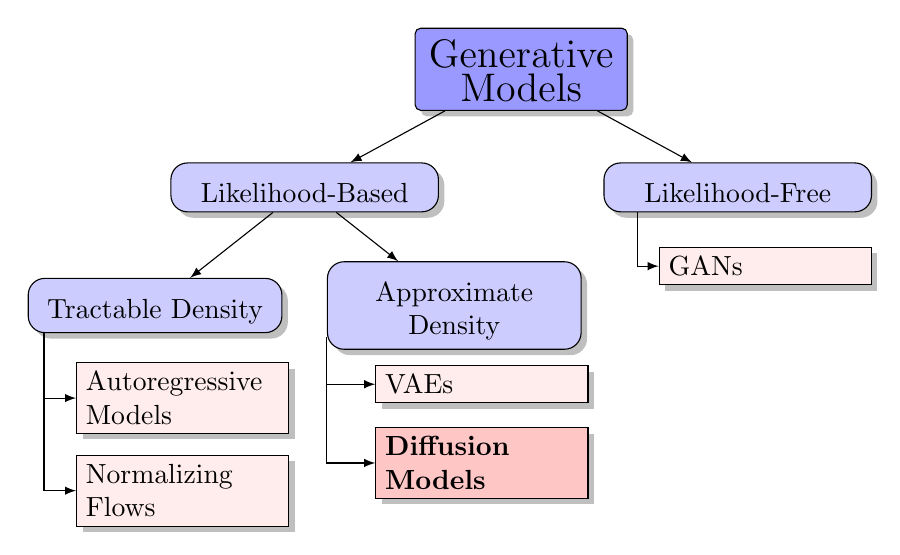
\begin{tikzpicture}[
        basic/.style  = {draw, text width=2cm, drop shadow, rectangle},
        root/.style   = {basic, rounded corners=2pt, thin, text height=1.1em, text width=7em, align=center, fill=blue!40},
        level 1/.style={sibling distance=55mm},
        level 2/.style = {basic, rounded corners=6pt, thin, align=center, fill=blue!20, text height=1.1em, text width=9em, sibling distance=38mm},
        level 3/.style = {basic, rounded corners=6pt, thin,align=center, fill=blue!20, text width=8.5em},
        level 4/.style = {basic, thin, align=left, fill=pink!30, text width=7em},
        level 5/.style = {basic, thin, align=left, fill=pink!90, text width=7em},
        edge from parent/.style={->,draw},
        >=latex]
        
        % root of the the initial tree, level 1
        \node[root] {\Large Generative Models}
        % The first level, as children of the initial tree
        child {node[level 2] (c1) {Likelihood-Based}
            child {node[level 3] (c11) {Tractable Density}}
            child {node[level 3] (c12) {Approximate Density}}
        }
        child {node[level 2] (c2) {Likelihood-Free}};
        
        % The second level, relatively positioned nodes
        \begin{scope}[every node/.style={level 4}]
            \node [below of = c11, yshift=-5pt, xshift=10pt] (c111) {Autoregressive Models};
            \node [below of = c111, yshift=-5pt] (c112) {Normalizing Flows};
            \node [below of = c12, xshift=10pt] (c121) {VAEs};
            
            \node [below of = c2, xshift=10pt] (c21) {GANs};
        \end{scope}
        
        % The second level, relatively positioned nodes
        \begin{scope}[every node/.style={level 5}]
            \node [below of = c121] (c122) {\textbf{Diffusion \\ Models}};
        \end{scope}
        
        % lines from each level 1 node to every one of its "children"
        \foreach \value in {1,2}
        \draw[->] (c11.194) |- (c11\value.west);
        
        \foreach \value in {1,2}
        \draw[->] (c12.194) |- (c12\value.west);
        
        \draw[->] (c2.194) |- (c21.west);
        
    \end{tikzpicture}
\end{frame}
%=======
\begin{frame}{Denoising Diffusion Probabilistic Model (DDPM)}
    \myfootnotewithlink{https://arxiv.org/abs/2006.11239}{Ho J. Denoising Diffusion Probabilistic Models, 2020}
    \begin{block}{DDPM is a VAE Model}
        \begin{itemize}
            \item The encoder is a fixed Gaussian Markov chain $q(\bx_1, \dots, \bx_T | \bx_0)$.
            \item The latent variable is hierarchical (at each step, its dimension equals the input's).
            \item The decoder is a simple Gaussian model $\pt(\bx_0 | \bx_1)$.
            \item The prior distribution is given by a parametric Gaussian Markov chain $\pt(\bx_{t-1} | \bx_t)$.
        \end{itemize}
    \end{block}
    \eqpause
    \begin{minipage}{0.5\linewidth}
        \begin{block}{Forward Process}
            \begin{enumerate}
                \item $\bx_0 = \bx \sim \pd(\bx)$;
                \item $\bx_t = \sqrt{1 - \beta_t} \cdot \bx_{t - 1} + \sqrt{\beta_t} \cdot \bepsilon$;
                \item $\bx_T \sim p_{\infty}(\bx) = \cN(0, \bI)$.
            \end{enumerate}
        \end{block}
    \end{minipage}%
    \eqpause
    \begin{minipage}{0.55\linewidth}
        \begin{block}{Reverse Process}
            \begin{enumerate}
                \item $\bx_T \sim p_{\infty}(\bx) = \cN(0, \bI)$;
                \item $\bx_{t - 1} = \bsigma_{\btheta, t}(\bx_t) \cdot \bepsilon + \bmu_{\btheta, t}(\bx_t)$;
                \item $\bx_0 = \bx \sim \pd(\bx)$;
            \end{enumerate}
        \end{block}
    \end{minipage}
\end{frame}
%=======
\begin{frame}{Denoising Diffusion Probabilistic Model (DDPM)}
    \myfootnotewithlink{https://arxiv.org/abs/2006.11239}{Ho J. Denoising Diffusion Probabilistic Models, 2020}
    \begin{block}{Training}
        \begin{enumerate}
            \item Obtain a sample $\bx_0 \sim \pd(\bx)$.
            \item Sample time index $t \sim U\{1, T\}$ and noise $\bepsilon \sim \cN(0, \bI)$.
            \item Generate noisy image $\bx_t = \sqrt{\bar{\alpha}_t} \cdot \bx_0 + \sqrt{1 - \bar{\alpha}_t} \cdot \bepsilon$.
            \item Compute the loss $ \cL_{\text{simple}} = \| \bepsilon - \bepsilon_{\btheta, t}(\bx_t) \|^2 $.
        \end{enumerate}
    \end{block}
    \eqpause
    \begin{block}{Sampling (Ancestral Sampling)}
        \begin{enumerate}
            \item Sample $\bx_T \sim \cN(0, \bI)$.
            \item Compute the mean of $\pt(\bx_{t-1} | \bx_t) = \cN(\bmu_{\btheta, t}(\bx_t), \tilde{\beta}_t \cdot \bI)$:
            \[
                \bmu_{\btheta, t}(\bx_t) = \frac{1}{\sqrt{\alpha_t}} \cdot \bx_t - \frac{1 - \alpha_t}{\sqrt{\alpha_t (1 - \bar{\alpha}_t)}} \cdot \bepsilon_{\btheta, t}(\bx_t)
            \]
            \vspace{-0.3cm}
            \item Denoise: $\bx_{t - 1} = \bmu_{\btheta, t}(\bx_t) +  \sqrt{\tilde{\beta}_t} \cdot \bepsilon$, $\bepsilon \sim \cN(0, \bI)$.
        \end{enumerate}
    \end{block}
\end{frame}
%=======
\begin{frame}{Denoising Diffusion Probabilistic Model (DDPM)}
    \myfootnotewithlink{https://arxiv.org/abs/2006.11239}{Ho J. Denoising Diffusion Probabilistic Models, 2020}
    \begin{block}{Samples}
        \begin{figure}
            \includegraphics[width=\linewidth]{../lecture8/figs/ddpm_samples}
        \end{figure}
    \end{block}
\end{frame}
%=======
\begin{frame}{Summary}
    \begin{itemize}
        \item DDPM approximates the reverse process using normality assumptions.     
        \vfill
        \item DDPM can be interpreted as a VAE with a hierarchy of latent variables.
        \vfill
        \item The ELBO for DDPM may be formulated as a sum over many KL divergence terms.
        \vfill
        \item At each step, DDPM predicts the noise that was injected in the forward process. 
        \vfill
        \item DDPM is a VAE model that tries to invert the forward diffusion process via variational inference. 
        \vfill
        \item DDPMs are quite slow, since the model must be applied $T$ times for sampling.
    \end{itemize}
\end{frame}
%=======

%================================================================================
% LECTURE 9
%================================================================================
\part{Lecture 9}
\createdgmtitle{9}

%--------------------------------------------------------------------------------
\begin{frame}[noframenumbering,plain]
\titlepage
    \resetonslide
\end{frame}
%=======
\begin{frame}{Recap of Lecture 7}
    \myfootnotewithlink{http://www.iro.umontreal.ca/~vincentp/Publications/smdae_techreport.pdf}{Vincent P. A Connection Between Score Matching and Denoising Autoencoders, 2010}

    Let us perturb the original data with Gaussian noise $q(\bx_{\sigma} | \bx) = \cN(\bx, \sigma^2 \cdot \bI)$.
    \vspace{-0.3cm}
    \[
        q(\bx_{\sigma}) = \int q(\bx_{\sigma} | \bx) \pd(\bx) d\bx.
    \]
    \vspace{-0.6cm} \\
    Then the solution of 
    \vspace{-0.2cm}
    \[
        \frac{1}{2} \bbE_{q(\bx_{\sigma})}\bigl\| \bs_{\btheta, \sigma}(\bx_{\sigma}) - \nabla_{\bx_{\sigma}} \log q(\bx_{\sigma}) \bigr\|^2_2 \rightarrow \min_{\btheta}
    \]
    \vspace{-0.5cm} \\
    satisfies $\bs_{\btheta, \sigma}(\bx_{\sigma}) \approx \bs_{\btheta, 0}(\bx_0) = \bs_{\btheta}(\bx)$ if $\sigma$ is sufficiently small.
    \begin{block}{Theorem (Denoising Score Matching)}
        \vspace{-0.8cm}
        \begin{multline*}
            \bbE_{q(\bx_{\sigma})}\bigl\| \bs_{\btheta, \sigma}(\bx_{\sigma}) - \nabla_{\bx_{\sigma}} \log q(\bx_{\sigma}) \bigr\|^2_2 = \\ = \bbE_{\pd(\bx)} \bbE_{q(\bx_{\sigma} | \bx)}\bigl\| \bs_{\btheta, \sigma}(\bx_{\sigma}) - \nabla_{\bx_{\sigma}} \log q(\bx_{\sigma} | \bx) \bigr\|^2_2 + \text{const}(\btheta)
        \end{multline*}
        \vspace{-0.7cm}
    \end{block}
    Here, $\nabla_{\bx_{\sigma}} \log q(\bx_{\sigma} | \bx) = - \frac{\bx_{\sigma} - \bx}{\sigma^2} = - \frac{\bepsilon}{\sigma}$. $\bs_{\btheta, \sigma}(\bx_{\sigma})$ attempts to \textbf{denoise} a corrupted sample.
\end{frame}
%=======
\begin{frame}{Recap of Lecture 7}
    \myfootnotewithlink{https://yang-song.github.io/blog/2021/score/}{Song Y. Generative Modeling by Estimating Gradients of the Data Distribution, blog post, 2021}
	\vspace{-0.5cm}
	\[
		\bbE_{\pd(\bx)} \bbE_{\cN(0, \bI)}\left\| \bs_{\btheta, \sigma}(\bx + \sigma \bepsilon) + \frac{\bepsilon}{\sigma} \right\|_2^2 \rightarrow \min_{\btheta}
	\]
	\begin{minipage}{0.5\linewidth}
		\[
			\bx_{l + 1} = \bx_l + \frac{\eta}{2} \cdot \bs_{\btheta, \sigma}(\bx_l) + \sqrt{\eta} \cdot \bepsilon_l
		\]
		\vspace{-0.3cm}
		\begin{itemize}
			\item For \textbf{small} $\sigma$, $\bs_{\btheta, \sigma}(\bx)$ becomes inaccurate and Langevin dynamics fails to traverse modes
			\item For \textbf{large} $\sigma$, robustness in low-density regions is achieved, but the model learns a distribution that is overly corrupted
		\end{itemize}
	\end{minipage}%
	\begin{minipage}{0.5\linewidth}
		\begin{figure}
			\includegraphics[width=\linewidth]{./../lecture7/figs/pitfalls}
		\end{figure}
		\vspace{-0.3cm}
		\begin{figure}
			\includegraphics[width=\linewidth]{./../lecture7/figs/single_noise}
		\end{figure}
	\end{minipage}
\end{frame}
%=======
\begin{frame}{Recap of Lecture 7}
    \myfootnotewithlink{https://arxiv.org/abs/1907.05600}{Song Y. et al. Generative Modeling by Estimating Gradients of the Data Distribution, 2019}
    \begin{block}{Noise-Conditioned Score Network}
        \begin{itemize}
            \item Define a sequence of noise levels: $\sigma_1 < \sigma_2 < \dots < \sigma_T$.
            \item Train a denoised score function $\bs_{\btheta, \sigma_t}(\bx_t)$ for each noise level:
            \vspace{-0.3cm}
            \[
                \sum_{t=1}^T {\color{violet}\sigma_t^2} \cdot \bbE_{\pd(\bx)} \bbE_{q(\bx_t | \bx)}\bigl\| \bs_{\btheta, \sigma_t}(\bx_t) - \nabla_{\bx_t} \log q(\bx_t | \bx) \bigr\|^2_2 \rightarrow \min_{\btheta}
            \]
            \vspace{-0.5cm}
            \item Sample using \textbf{annealed} Langevin dynamics (for $t=1, \dots, T$).
        \end{itemize}
    \end{block}
    \vspace{-0.3cm}
    \begin{figure}
        \includegraphics[width=0.55\linewidth]{./../lecture7/figs/multi_scale}
    \end{figure}
    \vspace{-0.3cm}
    \begin{figure}
        \includegraphics[width=\linewidth]{./../lecture7/figs/duoduo}
    \end{figure}
\end{frame}
%=======
\begin{frame}{Recap of Lecture 7}
    \myfootnotewithlink{https://arxiv.org/abs/2006.09011}{Song Y. et al. Improved Techniques for Training Score-Based Generative Models, 2020}
    \begin{block}{NCSN Training}
        \begin{enumerate}
            \item Obtain a sample $\bx_0 \sim \pd(\bx)$.
            \item Sample noise level $t \sim U\{1, T\}$ and noise $\bepsilon \sim \cN(0, \bI)$.
            \item Construct noisy image $\bx_t = \bx_0 + \sigma_t \cdot \bepsilon$.
            \item Compute the loss $ \cL = \sigma_t^2 \cdot \| \bs_{\btheta, \sigma_t}(\bx_t) + \frac{\bepsilon}{\sigma_t} \|^2 $.
        \end{enumerate}
    \end{block}
    \begin{block}{NCSN Sampling (Annealed Langevin Dynamics)}
        \begin{itemize}
            \item Sample $\bx_0 \sim \cN(0, \sigma_T^2 \cdot \bI) \approx q(\bx_T)$.
            \item Apply $L$ steps of Langevin dynamics:
            \vspace{-0.2cm}
            \[
                \bx_l = \bx_{l-1} + \frac{\eta_t}{2} \cdot \bs_{\btheta, \sigma_t}(\bx_{l - 1}) + \sqrt{\eta_t} \cdot \bepsilon_l.
            \] 
            \vspace{-0.5cm}
            \item Update $\bx_0 := \bx_L$ and proceed to the next $\sigma_t$.
        \end{itemize}
    \end{block}
\end{frame}
%=======
\begin{frame}{Recap of Lecture 7}
    \myfootnotewithlink{https://arxiv.org/abs/2403.18103}{Chan S. Tutorial on Diffusion Models for Imaging and Vision, 2024}
    \begin{block}{Forward Gaussian Diffusion Process}
        Let $\bx_0 = \bx \sim \pd(\bx)$, $\beta_t \ll 1$, $\alpha_t = 1 - \beta_t$ and $\bar{\alpha}_t = \prod_{s=1}^t \alpha_s$. 
        \begin{align*}
            \bx_t &= \sqrt{1 - \beta_t} \cdot \bx_{t - 1} + \sqrt{\beta_t} \cdot \bepsilon, \quad \text{where }\bepsilon \sim \cN(0, \bI); \\
            \bx_t &= \sqrt{\bar{\alpha}_t} \cdot \bx_{0} + \sqrt{1 - \bar{\alpha}_t} \cdot \bepsilon, \quad \text{where } \bepsilon \sim \cN(0, \bI).
        \end{align*}
        \vspace{-0.6cm}
        \begin{align*}
            q(\bx_t | \bx_{t-1}) &= \cN(\sqrt{1 - \beta_t} \cdot \bx_{t-1}, \beta_t \cdot \bI); \\
            q(\bx_t | \bx_0) &= \cN(\sqrt{\bar{\alpha}_t} \cdot \bx_0, (1 - \bar{\alpha}_t) \cdot \bI).
        \end{align*}
        \vspace{-0.6cm}
    \end{block}
    \begin{figure}
        \includegraphics[width=0.8\linewidth]{./../lecture7/figs/conditional_diffusion}
    \end{figure}
\end{frame}
%=======
\begin{frame}{Recap of Lecture 7}
    \myfootnotewithlink{https://ayandas.me/blog-tut/2021/12/04/diffusion-prob-models.html}{Das A. An Introduction to Diffusion Probabilistic Models, blog post, 2021}
    \textbf{Diffusion} describes the process where particles migrate from regions of high density to regions of low density.
    \vspace{-0.2cm}
    \begin{figure}
        \includegraphics[width=0.5\linewidth]{./../lecture7/figs/diffusion_over_time}
    \end{figure}
    \vspace{-0.6cm}
    \begin{enumerate}
        \item $\bx_0 = \bx \sim \pd(\bx)$;
        \item $\bx_t = \sqrt{1 - \beta_t} \cdot \bx_{t - 1} + \sqrt{\beta_t} \cdot \bepsilon$, with $\bepsilon \sim \cN(0, \bI)$, $t \geq 1$;
        \item $\bx_T \sim p_{\infty}(\bx) = \cN(0, \bI)$, for $T \gg 1$.
    \end{enumerate}
    If we can invert this process, we would have a way to sample $\bx \sim \pd(\bx)$ using noise samples, i.e. $p_{\infty}(\bx) = \cN(0, \bI)$. \\ 
    Hence, our objective becomes to reverse this process.
\end{frame}
%=======
\begin{frame}{Recap of Lecture 7}
    \myfootnotewithlink{https://lilianweng.github.io/posts/2021-07-11-diffusion-models/}{Weng L. What are Diffusion Models?, blog post, 2021}
    \vspace{-0.3cm}
    \begin{figure}
        \includegraphics[width=0.8\linewidth]{./../lecture7/figs/DDPM}
    \end{figure}
    \vspace{-0.5cm}
    \begin{block}{Reverse Process (Ancestral Sampling)}
        \vspace{-0.5cm}
        {\small
        \[
            q(\bx_{t-1}|\bx_{t}) = \frac{q(\bx_{t}|\bx_{t-1}) {\color{violet}q(\bx_{t-1})}}{{\color{violet}q(\bx_{t})}} \approx \pt(\bx_{t - 1} | \bx_t) = \cN \left(\bmu_{\btheta, t}(\bx_t), \bsigma_{\btheta, t}^2(\bx_t)\right)
        \]}
        {\color{gray}The Feller theorem guarantees this approximation is valid.}
    \end{block}
    \begin{minipage}{0.5\linewidth}
        \begin{block}{Forward Process}
            \begin{enumerate}
                \item $\bx_0 = \bx \sim \pd(\bx)$;
                \item $\bx_t = \sqrt{1 - \beta_t} \cdot \bx_{t - 1} + \sqrt{\beta_t} \cdot \bepsilon$;
                \item $\bx_T \sim p_{\infty}(\bx) = \cN(0, \bI)$.
            \end{enumerate}
        \end{block}
    \end{minipage}%
    \begin{minipage}{0.55\linewidth}
        \begin{block}{Reverse Process}
            \begin{enumerate}
                \item $\bx_T \sim p_{\infty}(\bx) = \cN(0, \bI)$;
                \item $\bx_{t - 1} = \bsigma_{\btheta, t}(\bx_t) \cdot \bepsilon + \bmu_{\btheta, t}(\bx_t)$;
                \item $\bx_0 = \bx \sim \pd(\bx)$;
            \end{enumerate}
        \end{block}
    \end{minipage}
\end{frame}





%=======
\begin{frame}{Outline}
	\tableofcontents[part=9]
\end{frame}
%=======
\section{DDPM as a Score-Based Generative Model}
%=======
\begin{frame}{Denoising Diffusion as a Score-Based Generative Model}
	\myfootnotewithlink{https://arxiv.org/abs/2006.11239}{Ho J. Denoising Diffusion Probabilistic Models, 2020}
	\begin{block}{DDPM Objective}
		\vspace{-0.7cm}
		\begin{align*}
			\cL_t &= \bbE_{\bepsilon \sim \cN(0, \bI)} \left[ C_{1, t} \cdot \left\|  \bepsilon_{\btheta, t} (\bx_t) - \bepsilon\right\|_2^2  \right] \\
			\nextonslide{
			& = \bbE_{\bepsilon \sim \cN(0, \bI)} \left[ C_{2, t} \cdot \Bigl\| {\color{violet} \frac{\bepsilon_{\btheta, t}  (\bx_t) }{\sqrt{1 - \bar{\alpha}_t}}} - {\color{teal}\frac{\bepsilon}{\sqrt{1 - \bar{\alpha}_t}}}\Bigr\|_2^2  \right]
			}
		\end{align*}
		\vspace{-0.7cm}
	\end{block}
	\eqpause
	\vspace{-0.5cm}
	\begin{align*}
		q(\bx_t | \bx_0) &= \cN(\sqrt{\bar{\alpha}_t} \cdot \bx_0, (1 - \bar{\alpha}_t) \cdot \bI) \\
		\nextonslide{\nabla_{\bx_t} \log q(\bx_t | \bx_0) &= - \frac{\bx_t - \sqrt{\bar{\alpha}_t} \cdot \bx_0}{1 - \bar{\alpha}_t} = {\color{teal}-  \frac{\bepsilon}{\sqrt{1 - \bar{\alpha}_t}}}.}
	\end{align*}
	\eqpause
	We can reparameterize the model as: 
		\vspace{-0.2cm}
		\[
			\bs_{\btheta, t}(\bx_t) = {\color{violet}- \frac{\bepsilon_{\btheta, t}(\bx_t)}{\sqrt{1 - \bar{\alpha}_t}}} = \nabla_{\bx_t} \log \pt(\bx_t).
		\]
		\vspace{-0.3cm}
		\eqpause
		\[
			\cL_t = \bbE_{q(\bx_t | \bx_0)} \left[ C_{2, t} \cdot \Bigl\|  \bs_{\btheta, t} (\bx_t) - \nabla_{\bx_t} \log q(\bx_t | \bx_0) \Bigr\|_2^2  \right]
		\]
\end{frame}
%=======
\begin{frame}{DDPM vs NCSN: Objectives}
	\myfootnotewithlink{https://arxiv.org/abs/2006.11239}{Ho J. Denoising Diffusion Probabilistic Models, 2020}
	\begin{block}{DDPM Objective}
		\vspace{-0.5cm}
		\[
			\bbE_{\pd(\bx_0)} \bbE_{t \sim U\{1, T\}}\bbE_{q(\bx_t | \bx_0)} \left[ {\color{olive}C_{2, t}} \Bigl\|  \bs_{\btheta, t} (\bx_t) - \nabla_{\bx_t} \log q(\bx_t | \bx_0) \Bigr\|_2^2  \right]
		\]
		\[
			\bx_t = \sqrt{\bar{\alpha}_t} \cdot \bx_0 + \sqrt{1 - \bar{\alpha}_t} \cdot \bepsilon
		\]
		\eqpause
		In practice, {\color{olive}this coefficient} is often omitted.
	\end{block}
	\eqpause
	\begin{block}{NCSN Objective}
		\vspace{-0.3cm}
		\[
			\bbE_{\pd(\bx_0)} \bbE_{t \sim U\{1, T\}} \bbE_{q(\bx_t | \bx_0)}\bigl\| \bs_{\btheta, \sigma_t}(\bx_t) - \nabla_{\bx_t} \log q(\bx_t | \bx_0) \bigr\|^2_2 
		\]
		\[
			\bx_t = \bx_0 + \sigma_t \cdot \bepsilon
		\]
		\vspace{-0.5cm}
	\end{block}
	\eqpause
	\textbf{Maximizing the ELBO leads to the same objective as denoising score matching!}
\end{frame}
%=======
\begin{frame}{DDPM vs NCSN: Sampling}
	\myfootnotewithlink{https://arxiv.org/abs/2006.11239}{Ho J. Denoising Diffusion Probabilistic Models, 2020}
	\begin{block}{DDPM Sampling (Ancestral Sampling)}
			\vspace{-0.7cm}
			\begin{align*}
				\bx_T &\sim \cN(0, \bI) \\
				\bx_{t - 1} &= {\color{teal}\bmu_{\btheta, t}(\bx_t)} + \sigma_t \cdot \bepsilon 
				\nextonslide{\\& ={\color{teal}\frac{1}{\sqrt{\alpha_t}} \cdot \bx_t - \frac{1 - \alpha_t}{\sqrt{\alpha_t (1 - \bar{\alpha}_t)}} \cdot \bepsilon_{\btheta, t}(\bx_t)} +  \sigma_t \cdot \bepsilon
				}
				\nextonslide{
				\\ & = \frac{1}{\sqrt{1 - \beta_t}} \cdot \bx_t + \frac{\beta_t}{\sqrt{1 - \beta_t}} \cdot \bs_{\btheta, t} (\bx_t) +  \sigma_t \cdot \bepsilon
				}
			\end{align*}
			\vspace{-0.5cm}
	\end{block}
	\eqpause
	\begin{block}{NCSN Sampling (Annealed Langevin Dynamics)}
		\begin{itemize}
			\item Sample $\bx_T^0 \sim \cN(0, \sigma_T^2\, \bI) \approx q(\bx_T)$.
			\item Perform $L$ steps of Langevin dynamics:
			\vspace{-0.2cm}
			\[
				\bx_t^l = \bx_t^{l-1} + \frac{\eta_t}{2} \cdot \bs_{\btheta, \sigma_t}(\bx_t^{l - 1}) + \sqrt{\eta_t} \cdot \bepsilon_t^l.
			\] 
			\vspace{-0.7cm}
			\item Set $\bx_{t-1}^0 = \bx_t^L$ and move to the next $\sigma_t$.
		\end{itemize}
	\end{block}
\end{frame}
%=======
\begin{frame}{DDPM vs NCSN: Summary}
	\myfootnote{\href{https://arxiv.org/abs/2107.00630}{Kingma D. et al. Variational Diffusion Models, 2021} \\
	\href{https://arxiv.org/abs/2011.13456}{Song Y. et al. Score-Based Generative Modeling through Stochastic Differential Equations, 2020}}
	\begin{block}{Summary}
		\begin{itemize}
		\item Different Markov chains:
			\begin{itemize}
				\item DDPM: $\bx_t = \sqrt{\bar{\alpha}_t} \cdot \bx_0 + \sqrt{1 - \bar{\alpha}_t} \cdot \bepsilon$;
				\item NCSN: $\bx_t = \bx_0 + \sigma_t \cdot \bepsilon$.
				\item One can generalize to $q(\bx_t |\bx_0) = \cN(\alpha_t \cdot \bx_0, \sigma^2_t\, \bI)$.
			\end{itemize}
		\eqpause
		\item The objectives coincide: ELBO $\equiv$ score-matching.
		\eqpause
		\item The sampling procedures differ:
			\begin{itemize}
				\item Ancestral sampling in DDPM;
				\item Annealed Langevin dynamics for NCSN;
				\item Hybrid approaches that combine both updates are possible.
			\end{itemize}
		\end{itemize}
	\end{block}
\end{frame}
%=======
\section{Guidance}
%=======
\begin{frame}{Guidance}
	\begin{itemize}
	\item Up to now, we have focused on \textbf{unconditional} generative models $\pt(\bx)$.
	\item In practice, most generative models are \textbf{conditional} (in diffusion era it is called guided): $\pt(\bx | \by)$.
	\item Here, $\by$ might denote a class label or \textbf{text} (as in text-to-image tasks).
	\end{itemize}
	\vspace{-0.3cm}
	\begin{minipage}[t]{0.5\columnwidth}
		\begin{figure}
			\includegraphics[width=0.9\linewidth]{../lecture9/figs/shedevrum1}
		\end{figure}
	\end{minipage}%
	\begin{minipage}[t]{0.5\columnwidth}
		\begin{figure}
			\includegraphics[width=0.9\linewidth]{../lecture9/figs/shedevrum2}
		\end{figure}
	\end{minipage}
\end{frame}
%=======
\begin{frame}{Conditional Models}
	In practice, we're typically interested in learning conditional models (sampling from conditional distribution~$\pd(\bx | \by)$). 
	\begin{itemize}
		\item $\by = \emptyset$, $\bx$ = image $\quad\Rightarrow\quad$ unconditional image model
		\item $\by$ = class label, $\bx$ = image $\quad\Rightarrow\quad$ class-conditional image model
		\item $\by$ = text prompt, $\bx$ = image $\quad\Rightarrow\quad$ text-to-image model
		\item $\by$ = image, $\bx$ = image $\quad\Rightarrow\quad$ image-to-image model
		\item $\by$ = image, $\bx$ = text $\quad\Rightarrow\quad$ image-to-text (image captioning) model
		\item $\by$ = English text, $\bx$ = Russian text $\quad\Rightarrow\quad$ sequence-to-sequence model (machine translation) model
		\item $\by$ = sound, $\bx$ = text $\quad\Rightarrow\quad$ speech-to-text (automatic speech recognition) model
		\item $\by$ = text, $\bx$ = sound $\quad\Rightarrow\quad$ text-to-speech model
	\end{itemize}
\end{frame}
%=======
\begin{frame}{Label Guidance}
	\myfootnotewithlink{https://arxiv.org/abs/1906.00446}{Razavi A., Oord A., et al. Generating Diverse High-Fidelity Images with VQ-VAE-2, 2019}
	\textbf{Label:} Ostrich (10th ImageNet class) 
	\begin{figure}
		\includegraphics[width=\linewidth]{../lecture9/figs/label_conditioning}
	\end{figure}
\end{frame}
%=======
\begin{frame}{Text Guidance}
	\myfootnotewithlink{https://arxiv.org/abs/2112.10741}{Nichol A., et al. GLIDE: Towards Photorealistic Image Generation and Editing with Text-Guided Diffusion Models, 2022}
	\textbf{Prompt:} a stained glass window of a panda eating bamboo \\
	Left: $\gamma = 1$, Right: $\gamma = 3$.
	\begin{figure}
		\includegraphics[width=\linewidth]{../lecture9/figs/cfg}
	\end{figure}
\end{frame}
%=======
\begin{frame}{Guidance in Generative Models}
	\begin{block}{How to make guided model?}
		Instead of sampling from $\pt(\bx)$, we sample from $\pt(\bx | \by)$.
	\end{block}
	\eqpause
	Given \textbf{supervised} data $\{(\bx_i, \by_i)\}_{i=1}^n$, we can treat $\by$ as an additional model input:
	\eqpause
	\begin{itemize}
		\item $\pt(x_j | \bx_{1:j-1}, {\color{olive}\by})$ for AR models;
		\eqpause
		\item Encoder $q_{\bphi}(\bz | \bx, {\color{olive}\by})$ and decoder $\pt(\bx | \bz, {\color{olive}\by})$ for VAEs;
		\eqpause
		\item $G_{\btheta}(\bz, {\color{olive}\by})$ for NFs and GANs;
		\eqpause
		\item $\pt(\bx_{t-1} | \bx_t, {\color{olive}\by})$ for DDPMs.
	\end{itemize}
	\eqpause
	\begin{block}{Challenge}
		\begin{itemize}
			\item Empirically, images sampled with this procedure do not fit well enough to the desired label $\by$.
			\item Being able to control the strength of guidance is especially valuable.
		\end{itemize}
	\end{block}
\end{frame}
%=======
\subsection{Classifier Guidance}
%=======
\begin{frame}{Classifier Guidance}
	\myfootnotewithlink{https://arxiv.org/abs/2105.05233}{Dhariwal P., Nichol A. Diffusion Models Beat GANs on Image Synthesis, 2021}
	\begin{block}{DDPM Sampling}
		\begin{enumerate}
			\item Sample $\bx_T \sim \cN(0, \bI)$.
			\item Generate the denoised image (unconditional generation):
			\vspace{-0.3cm}
			\begin{align*}
				\bx_{t - 1} &= \frac{1}{\sqrt{1 - \beta_t}} \cdot \bx_t + \frac{\beta_t}{\sqrt{1 - \beta_t}} \cdot {\color{teal}\bs_{\btheta, t} (\bx_t)} +  \sigma_t \cdot \bepsilon \\
				\nextonslide{
				& = \frac{1}{\sqrt{1 - \beta_t}} \cdot \bx_t + \frac{\beta_t}{\sqrt{1 - \beta_t}} \cdot {\color{teal} \nabla_{\bx_t} \log \pt(\bx_t)} +  \sigma_t \cdot \bepsilon
				}
			\end{align*}
			\vspace{-0.5cm}
		\end{enumerate}
	\end{block}
	\eqpause
	\begin{block}{Guided Generation}
		\vspace{-0.5cm}
		\[
			\bx_{t - 1} = \frac{1}{\sqrt{1 - \beta_t}}\cdot \bx_t +  \frac{\beta_t}{\sqrt{1 - \beta_t}}  \cdot  \nabla_{\bx_t} \log \pt(\bx_t | {\color{olive}\by}) +  \sigma_t \cdot \bepsilon
		\]
		\vspace{-0.3cm}
	\end{block}
	\eqpause
	What is the link between $\nabla_{\bx_t} \log \pt(\bx_t)$ and $\nabla_{\bx_t} \log \pt(\bx_t | {\color{olive}\by})$?
\end{frame}
%=======
\begin{frame}{Classifier Guidance: Guided Score Function}
	\myfootnotewithlink{https://arxiv.org/abs/2105.05233}{Dhariwal P., Nichol A. Diffusion Models Beat GANs on Image Synthesis, 2021}
	\begin{block}{Guided Generation}
		\vspace{-0.5cm}
		\[
			\bx_{t - 1} = \frac{1}{\sqrt{1 - \beta_t}}\cdot \bx_t +  \frac{\beta_t}{\sqrt{1 - \beta_t}}  \cdot {\color{olive} \nabla_{\bx_t} \log \pt(\bx_t | \by)} +  \sigma_t \cdot \bepsilon
		\]
		\vspace{-0.5cm}
	\end{block}
	\eqpause
	\begin{block}{Guided Generation}
		\vspace{-0.7cm}
		\begin{align*}
			{\color{olive}\nabla_{\bx_t} \log \pt(\bx_t | \by)} &= \nabla_{\bx_t} \log \left(\frac{\pt(\bx_t)p(\by | \bx_t)}{p(\by)} \right)\\
			\nextonslide{
			&= {\color{violet}\nabla_{\bx_t} \log \pt(\bx_t)} + \nabla_{\bx_t} \log p(\by | \bx_t) \\
			}
			\nextonslide{
			&= {\color{violet} \bs_{\btheta, t}(\bx_t)} + {\color{teal}\nabla_{\bx_t} \log p(\by | \bx_t)}
			}
		\end{align*}
	\end{block}
	\vspace{-0.5cm}
	\eqpause
	\begin{block}{Guided Score Function}
		\vspace{-0.3cm}
		\[
			\bs_{\btheta, t}(\bx_t, \by) = \nabla_{\bx_t} \log \pt(\bx_t | \by).
		\]
		\eqpause
		\vspace{-0.3cm}
		\[
			{\color{olive}\bs_{\btheta, t}(\bx_t, \by)} = {\color{violet}\bs_{\btheta, t}(\bx_t)} + {\color{teal}\nabla_{\bx_t} \log p(\by | \bx_t)}
		\]
	\end{block}
\end{frame}
%=======
\begin{frame}{Classifier Guidance: Guidance Scale}
	\myfootnotewithlink{https://arxiv.org/abs/2105.05233}{Dhariwal P., Nichol A. Diffusion Models Beat GANs on Image Synthesis, 2021}
	\begin{block}{Guided Score Function}
		\vspace{-0.3cm}
		\[
			{\color{olive}\bs_{\btheta, t}(\bx_t, \by)} = \bs_{\btheta, t}(\bx_t) + \nabla_{\bx_t} \log p(\by | \bx_t)
		\]
		\vspace{-0.5cm}
	\end{block}
	\eqpause
	\begin{itemize}
		\item Let us assume $\by$ is a class label.
		\item $p(\by | \bx_t)$ is a classifier for noisy inputs.
		\item $p(\by | \bx_t)$ is responsible for model guidance.
	\end{itemize}
	\eqpause
	\begin{block}{Guidance Scale}
		It is a natural idea to scale up the contribution of the guidance
		\[
			{\color{violet}\bs^{\gamma}_{\btheta, t}(\bx_t, \by)} = \bs_{\btheta, t}(\bx_t) + {\color{teal}\gamma} \cdot \nabla_{\bx_t} \log p(\by | \bx_t)
		\]
		\eqpause
		\vspace{-0.5cm}
		\begin{itemize}
			\item The {\color{teal}guidance scale $\gamma$} adjusts the strength of classifier guidance.
			\item ${\color{violet}\bs^{\gamma}_{\btheta, t}(\bx_t, \by)}$ is not the true guided score function ${\color{olive}\bs_{\btheta, t}(\bx_t, \by)}$.
		\end{itemize}
	\end{block}
\end{frame}
%=======
\begin{frame}{Classifier Guidance: Distribution Sharpening}
	\myfootnotewithlink{https://arxiv.org/abs/2105.05233}{Dhariwal P., Nichol A. Diffusion Models Beat GANs on Image Synthesis, 2021}
	\begin{block}{Scaled Guided Score Function}
		\[
			{\color{violet}\bs^{\gamma}_{\btheta, t}(\bx_t, \by)} = \bs_{\btheta, t}(\bx_t)+ {\color{teal}\gamma} \cdot \nabla_{\bx_t} \log p(\by | \bx_t)
		\]
		\vspace{-0.5cm}
	\end{block}
	\eqpause
	\begin{block}{Scaled Conditional Distribution}
		\vspace{-0.5cm}
		\begin{align*}
			{\color{violet}\nabla_{\bx_t}^{\gamma} \log \pt(\bx_t | \by)} 
			&= \nabla_{\bx_t} \log \pt(\bx_t) + {\color{teal}\gamma}  \cdot \nabla_{\bx_t} \log p(\by | \bx_t) \\
			\nextonslide{
			&= \nabla_{\bx_t} \log \pt(\bx_t) + \nabla_{\bx_t} \log p(\by | \bx_t)^{\color{teal}\gamma} \\
			}
			\nextonslide{
			&= \nabla_{\bx_t} \log \left( \frac{\pt(\bx_t) p(\by | \bx_t)^{\gamma}}{Z} \right)
			}
		\end{align*}
		\vspace{-0.3cm}
	\end{block}
	\eqpause
	\textbf{Note:} Increasing $\gamma$ sharpens $p(\by | \bx_t)$, making it more contrast
	\[
		\hat{p}(\by | \bx_t) \propto p(\by | \bx_t)^{\gamma}.
	\]
\end{frame}
%=======
\begin{frame}{Classifier Guidance: Overview}
	\myfootnotewithlink{https://arxiv.org/abs/2105.05233}{Dhariwal P., Nichol A. Diffusion Models Beat GANs on Image Synthesis, 2021}

	\begin{block}{Training}
		\begin{itemize}
			\item Train the DDPM as before.
			\item Train an additional classifier $p(\by | \bx_t)$ on noisy data (note that it is dependent on time $t$).
		\end{itemize}
		\vspace{-0.2cm}
	\end{block}
	\eqpause
	\begin{block}{Guided DDPM Sampling}
		\begin{enumerate}
			\item Sample $\bx_T \sim \cN(0, \bI)$.
			\item Generate the denoised image (using scaled guided score function):
			\[
				\bx_{t-1} = \frac{1}{\sqrt{1 - \beta_t}} \cdot \bx_t + \frac{\beta_t}{\sqrt{1 - \beta_t}} \cdot  {\color{olive}\bs^{\gamma}_{\btheta, t}(\bx_t, \by)} + \sigma_t \cdot \bepsilon
			\]
		\end{enumerate}
	\end{block}
\end{frame}
%=======
\subsection{Classifier-Free Guidance}
%=======
\begin{frame}{Classifier-Free Guidance}
	\myfootnotewithlink{https://arxiv.org/abs/2207.12598}{Ho J., Salimans T. Classifier-Free Diffusion Guidance, 2022}
	\begin{itemize}
		\item The previous approach relies on training an additional classifier $p(\by | \bx_t)$ for noisy images.	
		\item We now introduce a method to sidestep this requirement.
	\end{itemize}
	\eqpause
	\[
		\nabla_{\bx_t}^{\gamma} \log \pt(\bx_t | \by) = \nabla_{\bx_t} \log \pt(\bx_t) + \gamma \cdot {\color{teal}\nabla_{\bx_t} \log p(\by | \bx_t)}
	\]
	\eqpause
	\vspace{-0.5cm}
	\begin{block}{Bayes theorem}
		\vspace{-0.7cm}
		\begin{align*}
			{\color{teal}\nabla_{\bx_t} \log p(\by | \bx_t)} &= \nabla_{\bx_t} \log \left( \frac{\pt(\bx_t| \by) p(\by)}{\pt(\bx_t)} \right) \\
			\nextonslide{
			&=  \nabla_{\bx_t} \log \pt(\bx_t| \by) -\nabla_{\bx_t} \log  \pt(\bx_t)
			}
		\end{align*}
	\end{block}
	\eqpause
	\vspace{-0.5cm}
	\begin{block}{Scaled Guided Score Function}
		\vspace{-0.7cm}
		\begin{multline*}
			\nabla_{\bx_t}^{\gamma} \log \pt(\bx_t | \by) = \nabla_{\bx_t} \log \pt(\bx_t) + \gamma \cdot {\color{teal} \nabla_{\bx_t} \log p(\by | \bx_t)}
			\nextonslide{ = \\ = \nabla_{\bx_t} \log \pt(\bx_t) + \gamma \cdot \bigl( {\color{teal}\nabla_{\bx_t} \log \pt(\bx_t| \by) - \nabla_{\bx_t} \log  \pt(\bx_t)} \bigr)}
			\nextonslide{ = \\ =  (1 - \gamma) \cdot  \nabla_{\bx_t} \log \pt(\bx_t) + \gamma \cdot  \nabla_{\bx_t} \log \pt(\bx_t| \by)}
		\end{multline*}
	\end{block}
\end{frame}
%=======
\begin{frame}{Classifier-Free Guidance: Formulation}
	\myfootnotewithlink{https://arxiv.org/abs/2207.12598}{Ho J., Salimans T. Classifier-Free Diffusion Guidance, 2022}
	\begin{block}{Scaled Guided Score Function}
		\vspace{-0.5cm}
		\[
			\nabla_{\bx_t}^{\gamma} \log \pt(\bx_t | \by) =  (1 - \gamma) \cdot  \nabla_{\bx_t} \log \pt(\bx_t) + \gamma \cdot  \nabla_{\bx_t} \log \pt(\bx_t| \by)
		\]
		\vspace{-0.5cm}
		\eqpause
		\[
			\bs^{\gamma}_{\btheta, t}(\bx_t, \by) = (1 - \gamma) \cdot \bs_{\btheta, t}(\bx_t) +  \gamma \cdot \bs_{\btheta, t}(\bx_t, \by)
		\]
		\vspace{-0.5cm}
	\end{block}
	\eqpause
	\begin{block}{Naive training approach}
		\begin{itemize}
			\item Train an unguided score function model $\bs_{\btheta, t}(\bx_t)$.
			\item Train a guided score function model $\bs_{\btheta, t}(\bx_t, \by)$.
			\eqpause
			\item Use their convex combination at inference.
		\end{itemize}
	\end{block}
	\begin{block}{Guided Sampling}
		\vspace{-0.3cm}
		\[
			\bx_{t-1} = \frac{1}{\sqrt{1 - \beta_t}} \cdot \bx_t + \frac{\beta_t}{\sqrt{1 - \beta_t}} \cdot  {\color{olive}\bs^{\gamma}_{\btheta, t}(\bx_t, \by)} + \sigma_t \cdot \bepsilon
		\]
		\vspace{-0.3cm}
	\end{block}
	\eqpause
	How to avoid training two separate score function models?
\end{frame}
%=======
\begin{frame}{Classifier-Free Guidance}
	\myfootnotewithlink{https://arxiv.org/abs/2506.02070}{Holderrieth P., Erives E. An Introduction to Flow Matching and Diffusion Models, 2025}
	\[
		\bs^{\gamma}_{\btheta, t}(\bx_t, \by) = (1 - \gamma) \cdot \bs_{\btheta, t}(\bx_t) +  \gamma \cdot \bs_{\btheta, t}(\bx_t, \by)
	\]
	\vspace{-0.5cm}
	\begin{block}{CFG algorithm}
		\begin{itemize}
			\item Introduce "the absence of conditioning" label $\by = \varnothing$.		
			\eqpause
			\item Use it to get unguided score function $\bs_{\btheta, t}(\bx_t) = \bs_{\btheta, t}(\bx_t, \varnothing)$.		
			\eqpause
			\item Train a single model $\bs_{\btheta, t}(\bx_t, \by)$ using \textbf{supervised} data, but artificially drop the labels $\by$ with some fixed probability (simulating the case of $\by = \varnothing$).		
			\eqpause
			\item Apply the model twice during inference to get $\bs_{\btheta, t}(\bx_t, \varnothing)$ and $\bs_{\btheta, t}(\bx_t, \by)$.
		\end{itemize}
	\end{block}
	\vspace{-0.3cm}
	\eqpause
	\begin{block}{Guided Sampling}
		\vspace{-0.3cm}
		\[
			\bx_{t-1} = \frac{1}{\sqrt{1 - \beta_t}} \cdot \bx_t + \frac{\beta_t}{\sqrt{1 - \beta_t}} \cdot  {\color{olive}\bs^{\gamma}_{\btheta, t}(\bx_t, \by)} + \sigma_t \cdot \bepsilon
		\]
		\vspace{-0.3cm}
	\end{block}
\end{frame}
%=======
\section{Continuous-Time Normalizing Flows}
%=======
\begin{frame}{Discrete-Time Normalizing Flows}
	\myfootnotewithlink{https://lilianweng.github.io/lil-log/2018/10/13/flow-based-deep-generative-models.html}{https://lilianweng.github.io/lil-log/2018/10/13/flow-based-deep-generative-models.html}
	\vspace{-0.3cm}
	\begin{block}{Change of Variable Theorem (CoV)}
		Let $\bx$ be a random variable with density $p(\bx)$, and let $\bff: \bbR^m \rightarrow \bbR^m$ be a differentiable and \textbf{invertible} transformation. If $\bz = \bff(\bx)$, $\bx = \bff^{-1}(\bz) = \bg(\bz)$, then
		\vspace{-0.3cm}
		\[
			p(\bx) = p(\bz) |\det(\bJ_{\bff})| = p(\bz) \left|\det \left( \frac{\partial \bz}{\partial \bx} \right) \right| = p(\bff(\bx)) \left|\det \left(  \frac{\partial \bff(\bx)}{\partial \bx} \right) \right|
		\]
		\vspace{-0.5cm}
	\end{block}
	\eqpause

	\vspace{-0.3cm}
	\begin{figure}
		\includegraphics[width=0.95\linewidth]{../lecture9/figs/normalizing-flow}
	\end{figure}
	\vspace{-0.4cm}
	\[
		\log \pt(\bx) = \log p(\bff_K \circ \dots \circ \bff_1(\bx)) + \sum_{k=1}^K\log \left|\det \left(\frac{\partial \bff_k}{\partial \bff_{k-1}}\right)\right|.
	\]
	\vspace{-0.4cm}
\end{frame}
%=======
\begin{frame}{Towards Continuous-Time Normalizing Flows}
	\begin{itemize}
		\item Up to this point, we have considered discrete-time normalizing flows:
		\vspace{-0.3cm}
		 \[
		 	 \bx_{t+1} = \bff_{\btheta}(\bx_t, t); \quad \log p(\bx_{t+1}) = \log p(\bx_{t}) - \log \left| \det \frac{\partial \bff_{\btheta}(\bx_t)}{\partial \bx_{t}} \right| .
		 \]
		\item Let us now move to the general case of continuous time, using a mapping $\bx(t): \bbR \rightarrow \bbR^m$ to describe continuous dynamics.
	\end{itemize}
	\eqpause
	\begin{block}{Continuous-Time Dynamics}
		Consider an Ordinary Differential Equation (ODE):
		\vspace{-0.3cm}
		\begin{align*}
		   \frac{d \bx(t)}{dt} &= \bff_{\btheta}(\bx(t), t); \quad \text{with initial condition }\bx(t_0) = \bx_0. \\
		   \nextonslide{
		   \bx(t_1) &= \int^{t_1}_{t_0} \bff_{\btheta}(\bx(t), t) d t  + \bx_0
		   }
		\end{align*}
		\vspace{-0.6cm}
	\end{block}
	Here, $\bff_{\btheta}: \bbR^m \times [t_0, t_1] \rightarrow \bbR^m$ is a \textbf{vector field}.
\end{frame}
%=======
\begin{frame}{Ordinary Differential Equations (ODEs)}
	\begin{align*}
		\frac{d \bx(t)}{dt} &= \bff_{\btheta}(\bx(t), t); \quad \text{with initial condition }\bx(t_0) = \bx_0. \\
		\bx(t_1) &= \int^{t_1}_{t_0} \bff_{\btheta}(\bx(t), t) d t  + \bx_0
	\end{align*}
	\vspace{-0.6cm}
	\begin{block}{Flow}
		Let call \textbf{the flow} $\bpsi: \bbR^m \times [t_0, t_1] \rightarrow \bbR^m$ the solution of ODE:
		\[
			\frac{d \bpsi_t(\bx_0)}{dt} = \bff_{\btheta}(\bpsi_t(\bx_0), t); \quad \text{with initial condition }\bpsi_0(\bx_0) = \bx_0.
		\]
	\end{block}
	\begin{block}{Numerical Solution of ODEs}
		\vspace{-0.5cm}
		\[
			\bpsi_t(\bx_0) = \int^{t_1}_{t_0} \bff_{\btheta}(\bx(t), t) d t  + \bx_0 \nextonslide{\approx {\color{teal}\ODESolve_f(\bx_0, \btheta, t_0, t_1)}.}
		\]
		\eqpause
		Here, we require the numerical routine $\ODESolve_f(\bx_0, \btheta, t_0, t_1)$.
	\end{block}
\end{frame}
%=======
\begin{frame}{Numerical Solution of ODEs}
	\myfootnotewithlink{https://en.wikipedia.org/wiki/Heun's\_method}{Image credit: https://en.wikipedia.org/wiki/Heun's\_method}   
	\[
		\bpsi_t(\bx_0) = \int^{t_1}_{t_0} \bff_{\btheta}(\bx(t), t) d t  + \bx_0 \approx {\color{teal}\ODESolve_f(\bx_0, \btheta, t_0, t_1)}.
	\]
	$\ODESolve_f(\bx_0, \btheta, t_0, t_1)$ consists of sequence of iterative update steps.
	\eqpause
	\begin{block}{Euler Update Step}
		\begin{minipage}[t]{0.5\columnwidth}
			\vspace{-0.3cm}
			\[
	  			\frac{\bx(t + h) - \bx(t)}{h} = \bff_{\btheta}(\bx(t), t)
			\]
			\[
	  			\bx(t + h) = \bx(t) + h \cdot \bff_{\btheta}(\bx(t), t)
			\]
		\end{minipage}%
		\eqpause
		\begin{minipage}[t]{0.5\columnwidth}
			\vspace{-0.8cm}
			\begin{figure}
				\centering
				\includegraphics[width=\linewidth]{../lecture9/figs/heun_method}
			\end{figure}
		\end{minipage}
	\end{block}
	\vspace{-1.0cm}
	\begin{block}{Heun's Update Step}
		\vspace{-0.3cm}
		\[
			\bx'(t + h) = \bx(t) + h \cdot \bff_{\btheta}(\bx(t), t)
		\]
		\[
			\bx(t + h) = \bx(t) + \frac{h}{2} \cdot \left(\bff_{\btheta}(\bx(t), t) + \bff_{\btheta}(\bx'(t+h), t + h)\right)
		\]
	\end{block}
\end{frame}
%=======
\begin{frame}{Continuous-Time Normalizing Flows: Neural ODE}
	\myfootnotewithlink{https://arxiv.org/abs/1806.07366}{Chen R. T. Q. et al. Neural Ordinary Differential Equations, 2018}   
	\begin{block}{Neural ODE}
		\vspace{-0.2cm}
		\[
  			\frac{d \bx(t)}{dt} = \bff_{\btheta}(\bx(t), t); \quad \text{with initial condition }\bx(t_0) = \bx_0
		\]
		\vspace{-0.3cm}
	\end{block}
	\begin{block}{Euler \ODESolve}
		\vspace{-0.3cm}
		\[
		    \bx(t + h) = \bx(t) + h \cdot \bff_{\btheta}(\bx(t), t)
		\]
		\vspace{-0.5cm}
	\end{block}
	\eqpause
	\begin{itemize}
		\item Consider $[t_0, t_1] = [0, 1]$ for simplicity.
		\item If $\bx(0)$ is a random variable with density~$p_0(\bx)$,
		\item Then, for any $t$, $\bx(t)$ is a random variable with density $p_t(\bx)$.
	\end{itemize}
\end{frame}
%=======
\begin{frame}{Continuous-Time Normalizing Flows: Intuition}
	\myfootnotewithlink{https://arxiv.org/abs/1810.01367}{Grathwohl W. et al. FFJORD: Free-form Continuous Dynamics for Scalable Reversible Generative Models, 2018}  
	\[
 		\frac{d \bx(t)}{dt} = \bff_{\btheta}(\bx(t), t); \quad \text{with initial condition }\bx(t_0) = \bx_0
	\]
	\eqpause
	\vspace{-0.5cm}
	\begin{itemize}
		\item $p_t(\bx) = p(\bx, t)$ describes the \textbf{probability path} interpolating between $p_0(\bx)$ and $p_1(\bx)$.
		\item {\color{gray}What is the difference between $p_t(\bx(t))$ and $p_t(\bx)$?}
	\end{itemize}
	\eqpause
	\begin{figure}
		\centering
		\includegraphics[width=0.75\linewidth]{../lecture9/figs/cnf_flow.png}
	\end{figure}
\end{frame}
%=======
\begin{frame}{Continuous-Time Normalizing Flows: Reversibility}
	\myfootnotewithlink{https://arxiv.org/abs/1806.07366}{Chen R. T. Q. et al. Neural Ordinary Differential Equations, 2018}   
	\begin{block}{Theorem (Picard)}
		If $\bff$ is continuously differentiable with a bounded derivative in $\bx$ and continuous in $t$, then the ODE has a \textbf{unique solution} given by a flow $\bpsi_t$.
	\end{block}
	\eqpause
	This guarantees the ODE is \textbf{uniquely reversible}. 
	\vspace{-0.3cm}
	\begin{align*}
		\bpsi_1(\bx_0) &= \bx_0 + \int_{0}^{1} \bff_{\btheta}(\bpsi_t(\bx_0), t) dt \\
		\bx(1) &= \bx(0) + \int_{0}^{1} \bff_{\btheta}(\bx(t), t) dt \\
		\bx(0) &= \bx(1) + \int_{1}^{0} \bff_{\btheta}(\bx(t), t) dt
	\end{align*}
	\eqpause
	\textbf{Note:} Unlike discrete-time flows, $\bff$ need not be invertible (uniqueness ensures bijection).
	\eqpause
	How can we compute $p_t(\bx)$ at arbitrary $t$?
\end{frame}
%=======
\begin{frame}{Summary}
	\begin{itemize}
		\item DDPM and NCSN are intimately connected at the objective level.	
		\vfill
		\item Classifier guidance provides a technique to turn an unconditional model into a conditional one by training an auxiliary classifier on noisy data.
		\vfill
		\item Classifier-free guidance removes the need for such a classifier, yielding a practical recipe now widely used.
		\vfill 
		\item Continuous-time normalizing flows leverage neural ODEs to define continuous-time trajectories $\bx(t)$, relaxing many constraints of discrete-time flows.
		\vfill
		\item If $\bx_0$ is a random variable, this yields a \textbf{probability path} $p_t(\bx)$ as time evolves.
	\end{itemize}
\end{frame}
%=======

%================================================================================
% LECTURE 10
%================================================================================
\part{Lecture 10}
\createdgmtitle{10}

%--------------------------------------------------------------------------------
\begin{frame}[noframenumbering,plain]
\titlepage
	\resetonslide	
\end{frame}







%=======
\begin{frame}{Outline}
	\tableofcontents[part=10]
\end{frame}
%=======
\section{Continuity Equation for NF Log-Likelihood}
%=======
\begin{frame}{Continuous-Time NF}
	\myfootnotewithlink{https://arxiv.org/abs/1806.07366}{Chen R. T. Q. et al. Neural Ordinary Differential Equations, 2018}   
	\begin{block}{Theorem (Continuity Equation)}
		If $\bff$ is uniformly Lipschitz continuous in $\bx$ and continuous in $t$, then
		\[
			\frac{d \log p_t(\bx(t))}{d t} = - \tr \left( \frac{\partial \bff(\bx(t), t)}{\partial \bx(t)} \right)
		\]
		\vspace{-0.3cm}
	\end{block}
	\eqpause
	This result states: given $\bx_0 = \bx(0)$, the solution to the continuity equation gives the density $p_1(\bx(1))$.
	\begin{block}{Solution of the Continuity Equation}
		\vspace{-0.3cm}
		\[
			\log p_1(\bx(1)) = \log p_0(\bx(0)) - {\color{teal}\int_{0}^{1} \tr  \left( \frac{\partial \bff(\bx(t), t)}{\partial \bx(t)} \right) dt}.
		\]
		\vspace{-0.3cm}
	\end{block}
	\eqpause
	\begin{itemize}
		\item This provides the density along the trajectory (not the total probability path).
		\item However, {\color{teal}the latter term} is difficult to estimate efficiently.
	\end{itemize}
\end{frame}
%=======
\section{SDE Basics}
%=======
\begin{frame}{Stochastic Differential Equation (SDE)}
	\myfootnotewithlink{https://arxiv.org/abs/2506.02070}{Holderrieth P., Erives E. An Introduction to Flow Matching and Diffusion Models, 2025}
	\vspace{-0.3cm}
	\begin{block}{Wiener Process}
		$\bw(t)$ is the standard Wiener process (Brownian motion), defined~by:
		\vspace{-0.3cm}
		\begin{minipage}{0.5\columnwidth}
			\begin{enumerate}
				\item $\bw(0) = 0$ (almost surely);
				\item $\bw(t)$ has independent increments;
				\item $\bw(t)$ trajectories are continuous;
				\item $\bw(t) - \bw(s) \sim \cN(0, (t-s) \bI)$ for $t>s$;
			\end{enumerate}
		\end{minipage}%
		\begin{minipage}{0.45\columnwidth}
			\centering
			\includegraphics[width=\linewidth]{../lecture10/figs/brownian_motion}
		\end{minipage}
	\end{block}
	\vspace{0.3cm}
	\eqpause
	$d\bw = \bw(t+dt) - \bw(t) = \cN(0, \bI \cdot dt ) = \bepsilon \cdot \sqrt{dt}$, where $\bepsilon \sim \cN(0, \bI)$.
\end{frame}
%=======
\begin{frame}{Stochastic Differential Equation (SDE)}
	\[
 		\frac{d \bx}{dt} = \bff(\bx, t) \Rightarrow d\bx = \bff(\bx, t) dt
	\]
	\eqpause
	Let's define a stochastic process $\bx(t)$ with initial condition $\bx(0) \sim p_0(\bx) = \pd(\bx)$:
	\[
		d\bx = \bff(\bx, t) dt + {\color{violet}g(t) d \bw}
	\]
	\eqpause
	\vspace{-0.5cm}
	\begin{itemize}
		 \item $\bff(\bx, t): \bbR^m \times [0, 1] \rightarrow \bbR^m$ is the \textbf{drift} term (vector field).
		 \item $g(t): \bbR \rightarrow \bbR$ is the \textbf{diffusion} term (if $g(t)=0$, we recover the standard ODE).
		 \item $\bw(t)$ is the standard Wiener process ($d\bw = \bepsilon \cdot \sqrt{dt}$).
		 \item We do not have the flow $\bpsi_t(\bx_0)$ notion anymore, since trajectories are stochastic.
	\end{itemize}
\end{frame}
%=======
\begin{frame}{Stochastic Differential Equation (SDE)}
	\[
		d\bx = \bff(\bx, t) dt + g(t) d \bw
	\]
	\begin{block}{Theorem}
		If $\bff$ is continuously differentiable with a bounded derivative in $\bx$ 
		and continuous in $t$ and $g(t)$ is continuous then the SDE has the solution given by unique process $\bx(t)$.
	\end{block}

	\begin{itemize}
		\item Unlike ODEs, the initial condition $\bx(0)$ doesn't uniquely determine the trajectory.
		\item There are two sources of randomness: 
		\begin{itemize}
			\item the initial distribution $p_0(\bx)$;
			\item the Wiener process $\bw(t)$.
		\end{itemize}
	\end{itemize}
\end{frame}
%=======
\begin{frame}{Stochastic Differential Equation (SDE)}
	\[
		d\bx = \bff(\bx, t) dt + g(t) d \bw
	\]
	\vspace{-0.3cm}
	\eqpause
	\begin{block}{Discretizing the SDE (Euler Update Step) – \SDESolve}
		\vspace{-0.3cm}
		\[
			{\color{violet}\bx(t + dt) = \bx(t) + \bff(\bx(t), t) \cdot dt} + {\color{teal}g(t) \cdot \bepsilon \cdot \sqrt{dt}}
		\]
		If $dt=1$, then
		\vspace{-0.3cm}
		\[
			{\color{violet}\bx_{t + 1} = \bx_t + \bff(\bx_t, t)} + {\color{teal}g(t) \cdot \bepsilon}
		\]
		\vspace{-0.7cm}
	\end{block}
	\eqpause
	\begin{itemize}
		\item At any time $t$, the process has density $p_t(\bx) = p(\bx, t)$.
		\item $p: \bbR^m \times [0,1] \rightarrow \bbR_+$ specifies a \textbf{probability path} from $p_0(\bx)$ to $p_1(\bx)$.
		\item How can we obtain the probability path $p_t(\bx)$ for $\bx(t)$?
	\end{itemize}
\end{frame}
%=======
\begin{frame}{Stochastic Differential Equation (SDE)}
	\vspace{-0.4cm}
	\[
		d\bx = \bff(\bx, t) dt + g(t) d \bw,\quad d \bw = \bepsilon \cdot \sqrt{dt},\quad \bepsilon \sim \cN(0, \bI).
	\]
	\vspace{-0.4cm}
	\begin{block}{Theorem (Kolmogorov-Fokker-Planck)}
		The evolution of $p_t(\bx)$ is governed by
		\vspace{-0.2cm}
		\[
			\frac{\partial p_t(\bx)}{\partial t} = - \diver\left(\bff(\bx, t) p_t(\bx)\right) + \frac{1}{2}g^2(t) \Delta_{\bx}p_t(\bx)
		\]
		\eqpause
		Here,
		\[
			\diver (\bv) = \sum_{i=1}^m \frac{\partial v_i(\bx)}{\partial x_i} = \tr\left( \frac{\partial \bv(\bx)}{\partial \bx}  \right)
		\]
		\[
			\Delta_{\bx}p_t(\bx) = \sum_{i=1}^m \frac{\partial^2 p_t(\bx)}{\partial x_i^2} = \tr\left( \frac{\partial^2 p_t(\bx)}{\partial \bx^2}  \right)
		\]
		\eqpause
		\[
			\frac{\partial p_t(\bx)}{\partial t} = \tr\left( - \frac{\partial}{\partial \bx} \bigl[ \bff(\bx, t) p_t(\bx)\bigr] + \frac{1}{2} g^2(t) \frac{\partial^2 p_t(\bx)}{\partial \bx^2} \right)
		\]
	\end{block}
\end{frame}
%=======
\begin{frame}{Stochastic Differential Equation (SDE)}
	\begin{block}{Theorem (Kolmogorov-Fokker-Planck)}
		\vspace{-0.2cm}
		\[
			\frac{\partial p_t(\bx)}{\partial t} = \tr\left( - \frac{\partial}{\partial \bx} \bigl[ \bff(\bx, t) p_t(\bx)\bigr] + \frac{1}{2} g^2(t) \frac{\partial^2 p_t(\bx)}{\partial \bx^2}\right)
		\]
		\vspace{-0.2cm}
	\end{block}
	\begin{itemize}
		\item The KFP theorem is necessary and sufficient condition (it is uniquely defines $p_t(\bx)$).
		\item This generalizes the continuity equation for continuous-time NF:
		\[
			\frac{d \log p_t(\bx(t))}{d t} = - \tr \left( \frac{\partial \bff(\bx, t)}{\partial \bx} \right).
		\]
	\end{itemize}
	\eqpause
	\vspace{-0.3cm}
	\begin{block}{Special Case: constant density $p_t(\bx)$}
		Let find the SDE for which $p_t(\bx) = \text{const}$ (i.e., if $\bx(0) \sim p_0(\bx)$, then $\bx(t) \sim p_0(\bx)$.).
		\eqpause
		\[
			\frac{\partial p_t(\bx)}{\partial t} = 0 \quad \Leftrightarrow \quad \tr\left( - \frac{\partial}{\partial \bx} \bigl[ \bff(\bx, t) p_t(\bx)\bigr] + \frac{1}{2} g^2(t) \frac{\partial^2 p_t(\bx)}{\partial \bx^2}\right) = 0
		\]
	\end{block}
\end{frame}
%=======
\begin{frame}{Langevin SDE (Special Case)}
	\[
		\frac{\partial p_t(\bx)}{\partial t} = 0 \quad \Leftrightarrow \quad \tr\left( - \frac{\partial}{\partial \bx} \bigl[ \bff(\bx, t) p_t(\bx)\bigr] + \frac{1}{2} g^2(t) \frac{\partial^2 p_t(\bx)}{\partial \bx^2}\right) = 0
	\]
	\vspace{-0.3cm}
	\eqpause
	\[
		\frac{\partial}{\partial \bx} \bigl[ \bff(\bx, t) p_t(\bx)\bigr] = \frac{1}{2} g^2(t) \frac{\partial^2 p_t(\bx)}{\partial \bx^2}
	\]
	\eqpause
	\[
		\bff(\bx, t) p_t(\bx) = \frac{1}{2} g^2(t) \frac{\partial p_t(\bx)}{\partial \bx}
	\]
	\eqpause
	\[
		\bff(\bx, t) = \frac{1}{2} g^2(t) \frac{1}{p_t(\bx)}\frac{\partial p_t(\bx)}{\partial \bx} = \frac{1}{2} g^2(t) \frac{\partial}{\partial \bx} \log p_t(\bx)
	\]
	\eqpause
	Let ${\color{olive}g(t)=1}$, then ${\color{violet}\bff(\bx, t) = \frac{1}{2} \frac{\partial}{\partial \bx} \log p_t(\bx)}$.
	\[
		d \bx = {\color{violet}\frac{1}{2} \frac{\partial}{\partial \bx} \log p_t(\bx) d t} + {\color{olive}1} \cdot d \bw
	\]
\end{frame}
%=======
\begin{frame}{Langevin SDE (Special Case)}
	Let find the SDE for which $p_t(\bx) = \text{const}$ (i.e., if $\bx(0) \sim p_0(\bx)$, then $\bx(t) \sim p_0(\bx)$.).
	\[
		d \bx = {\color{violet}\frac{1}{2} \frac{\partial}{\partial \bx} \log p_t(\bx) d t} + {\color{olive}1} \cdot d \bw
	\]
	\eqpause
	\begin{block}{Discretized Langevin SDE}
		\vspace{-0.3cm}
		\[
			\bx_{t + 1} - \bx_t = \frac{\eta}{2} \cdot \frac{\partial}{\partial \bx} \log p_t(\bx) + \sqrt{\eta} \cdot \bepsilon, \quad \eta \approx dt.
		\]
		\vspace{-0.4cm}
	\end{block}
	\begin{block}{Langevin Dynamic}
		\vspace{-0.3cm}
		\[
			\bx_{t + 1} = \bx_t + \frac{\eta}{2} \cdot \nabla_{\bx} \log \pt(\bx) + \sqrt{\eta} \cdot \bepsilon, \quad \eta \approx dt.
		\]
		\vspace{-0.3cm}
	\end{block}
	We (partially) explained, why Langevin dynamics is working.
\end{frame}
%=======
\section{Probability Flow ODE}
%=======
\begin{frame}{Probability Flow ODE}
	\myfootnotewithlink{https://arxiv.org/abs/2011.13456}{Song Y., et al. Score-Based Generative Modeling through Stochastic Differential Equations, 2020}
	\begin{block}{ODE and Continuity Equation}
		\vspace{-0.3cm}
		\[
			d\bx = \bff(\bx, t) dt
		\]
		\[
			\frac{d \log p_t(\bx(t))}{d t} = - \tr \left( \frac{\partial \bff_{\btheta}(\bx, t)}{\partial \bx} \right) 
			\quad  \Leftrightarrow  \quad 
 			\frac{\partial p_t(\bx)}{\partial t} = - \diver(\bff(\bx, t) p_t(\bx))
 		\]
		The only source of randomness is the initial distribution $p_0(\bx)$.
	\end{block}
	\eqpause
	\begin{block}{SDE and KFP Equation}
		\vspace{-0.3cm}
		\[
			d\bx = \bff(\bx, t) dt + g(t) d \bw
		\]
 		\[
 			\frac{\partial p_t(\bx)}{\partial t} = - \diver(\bff(\bx, t) p_t(\bx)) + \frac{1}{2}g^2(t) \Delta_{\bx}p_t(\bx)
 		\]
		Now there are two sources of randomness: the initial distribution $p_0(\bx)$ and the Wiener process $\bw(t)$.
	\end{block}
\end{frame}
%=======
\begin{frame}{Probability Flow ODE}
	\myfootnotewithlink{https://arxiv.org/abs/2011.13456}{Song Y., et al. Score-Based Generative Modeling through Stochastic Differential Equations, 2020}
	\begin{block}{Theorem}
		Suppose the SDE $d\bx = \bff(\bx, t) dt + g(t) d \bw$ induces the probability path $p_t(\bx)$.
		Then, there exists an ODE with the same probability path $p_t(\bx)$, given by
		\vspace{-0.3cm}
		\[
			d\bx = \left(\bff(\bx, t) -\frac{1}{2} g^2(t) \frac{\partial}{\partial \bx} \log p_t(\bx) \right) dt
		\]
		\vspace{-0.7cm}
	\end{block}
	\eqpause
	\begin{figure}
		\includegraphics[width=0.75\linewidth]{../lecture10/figs/probability_flow}
	\end{figure}
\end{frame}
%=======
\begin{frame}{Probability Flow ODE}
	\myfootnotewithlink{https://arxiv.org/abs/2011.13456}{Song Y., et al. Score-Based Generative Modeling through Stochastic Differential Equations, 2020}
	\vspace{-0.3cm}
	\begin{block}{Theorem}
		Suppose the SDE $d\bx = \bff(\bx, t) dt + g(t) d \bw$ induces the probability path $p_t(\bx)$.
		Then, there exists an ODE with the same probability path $p_t(\bx)$, given by
		\vspace{-0.3cm}
		\[
			d\bx = \left(\bff(\bx, t) -\frac{1}{2} g^2(t) \frac{\partial}{\partial \bx} \log p_t(\bx) \right) dt
		\]
		\vspace{-0.7cm}
	\end{block}
	\begin{block}{Proof}
 		\vspace{-0.7cm}
 		{\small
 		\begin{multline*}
 			\frac{\partial p_t(\bx)}{\partial t} = \tr\left( - \frac{\partial}{\partial \bx} \bigl[ \bff(\bx, t) p_t(\bx)\bigr] + \frac{1}{2} g^2(t) \frac{\partial^2 p_t(\bx)}{\partial \bx^2} \right) 
			\nextonslide{= \\ = \tr\left( - \frac{\partial}{\partial \bx} \left[ \bff(\bx, t) p_t(\bx) - \frac{1}{2} g^2(t) {\color{violet}\frac{\partial p_t(\bx)}{\partial \bx}} \right]  \right)}
			\nextonslide{ = \\ =  \tr\left( - \frac{\partial}{\partial \bx} \left[ \bff(\bx, t) p_t(\bx) - \frac{1}{2} g^2(t) {\color{violet}p_t(\bx) \frac{\partial}{\partial \bx} \log p_t(\bx)} \right]  \right)}
			\nextonslide{= \\ =  \tr\left( - \frac{\partial}{\partial \bx} \left[ \left( {\color{teal}\bff(\bx, t) - \frac{1}{2} g^2(t) \frac{\partial}{\partial \bx} \log p_t(\bx)}\right) p_t(\bx) \right]  \right)}
 		\end{multline*}
 		}
 	\end{block}
\end{frame}
%=======
\begin{frame}{Probability Flow ODE}
	\myfootnotewithlink{https://arxiv.org/abs/2011.13456}{Song Y., et al. Score-Based Generative Modeling through Stochastic Differential Equations, 2020}
	\begin{block}{Proof (Continued)}
 		\vspace{-0.7cm}
 		\begin{multline*}
 			\frac{\partial p_t(\bx)}{\partial t} =  \tr\left( - \frac{\partial}{\partial \bx} \left[ \left( {\color{teal}\bff(\bx, t) - \frac{1}{2} g^2(t) \frac{\partial}{\partial \bx}\log p_t(\bx)}\right) p_t(\bx) \right]  \right) 
			\nextonslide{=\\ =  \tr\left( - \frac{\partial}{\partial \bx} \left[ {\color{teal}\tilde{\bff}(\bx, t)} p_t(\bx) \right]  \right) = -  \diver\left(\tilde{\bff}(\bx, t) p_t(\bx)\right)}
 		\end{multline*}
		\eqpause
		\[
			\tilde{\bff}(\bx, t) = \bff(\bx, t) -\frac{1}{2} g^2(t) \frac{\partial}{\partial \bx} \log p_t(\bx); \quad \tilde{g}(t) = 0
		\]
	 	\[
	 		d \bx = \tilde{\bff}(\bx, t) dt + 0 \cdot d \bw = \left(\bff(\bx, t) -\frac{1}{2} g^2(t) \frac{\partial}{\partial \bx} \log p_t(\bx) \right) dt
	 	\]
		\[
			\frac{\partial p_t(\bx)}{\partial t} = - \diver(\tilde{\bff}(\bx, t) p_t(\bx)) + \frac{1}{2}\tilde{g}^2(t) \Delta_{\bx}p_t(\bx)
		\]
 	\end{block}
\end{frame}
%=======
\begin{frame}{Probability Flow ODE}
	\myfootnotewithlink{https://arxiv.org/abs/2011.13456}{Song Y., et al. Score-Based Generative Modeling through Stochastic Differential Equations, 2020}
	\vspace{-0.3cm}
	\begin{align*}
		d\bx &= \bff(\bx, t) dt + g(t) d \bw \;\; - \text{SDE} \\
		d\bx &= \left(\bff(\bx, t) -\frac{1}{2} g^2(t) \frac{\partial}{\partial \bx} \log p_t(\bx) \right) dt  \;\; - \text{Probability Flow ODE}
	\end{align*}
	\eqpause
	\vspace{-0.5cm}
	\begin{itemize}
		\item The term $\bs(\bx, t) = \frac{\partial}{\partial \bx} \log p_t(\bx)$ is the score function in continuous time.
		\eqpause
		\item The ODE produces more stable trajectories.
	\end{itemize}
	\vspace{-0.3cm}
	\begin{figure}
		\includegraphics[width=0.75\linewidth]{../lecture10/figs/probability_flow}
	\end{figure}
\end{frame}
%=======
\section{Reverse SDE}
%=======
\begin{frame}{Reverse SDE}
	\myfootnotewithlink{https://arxiv.org/abs/2011.13456}{Song Y., et al. Score-Based Generative Modeling through Stochastic Differential Equations, 2020}
	\vspace{-0.3cm}
	\[
		d\bx = \bff(\bx, t) dt,\qquad \bx(t + dt) = \bx(t) + \bff(\bx, t) dt
	\]
	Here $dt$ can be $>0$ or $<0$.
	\eqpause
	\begin{block}{Reverse ODE}
		Let $\tau = 1 - t$ ($d\tau = -dt$).
		\vspace{-0.3cm}
		\[
			d\bx = - \bff(\bx, 1 - \tau) d\tau
		\]
	\end{block}
	\eqpause
	\vspace{-0.5cm}
	\begin{itemize}
		\item How do we reverse the SDE $d\bx = \bff(\bx, t) dt + g(t) d \bw$? 
		\item The Wiener process introduces randomness that must be reversed.
	\end{itemize}
	\eqpause
	\vspace{-0.3cm}
	\begin{block}{Theorem}
		There exists a reverse SDE for $d\bx = \bff(\bx, t) dt + g(t) d \bw$, given by:
		\vspace{-0.3cm}
		\[
			d\bx = \left(\bff(\bx, t) {\color{violet}- g^2(t) \frac{\partial}{\partial \bx}\log p_t(\bx)}\right) dt + g(t) d \bw
		\]
		\vspace{-0.5cm}\\
		where $dt<0$.
	\end{block}
\end{frame}
%=======
\begin{frame}{Reverse SDE}
	\myfootnotewithlink{https://arxiv.org/abs/2011.13456}{Song Y., et al. Score-Based Generative Modeling through Stochastic Differential Equations, 2020}
	\begin{block}{Theorem}
		There exists a reverse SDE for $d\bx = \bff(\bx, t) dt + g(t) d \bw$, given by:
		\vspace{-0.3cm}
		\[
			d\bx = \left(\bff(\bx, t) {\color{violet}- g^2(t) \frac{\partial}{\partial \bx}\log p_t(\bx)}\right) dt + g(t) d \bw
		\]
		\vspace{-0.5cm}\\
		where $dt<0$.
	\end{block}
	\eqpause
	\textbf{Note:} Again, the score function appears: $\bs(\bx, t) = \frac{\partial}{\partial \bx} \log p_t(\bx)$.
	\begin{block}{Proof Sketch}
		\begin{itemize}
			\item Convert the initial SDE to a probability flow ODE.
			\item Reverse the probability flow ODE.
			\item Convert the reversed probability flow ODE back to an SDE.
		\end{itemize}
	\end{block}
\end{frame}
%=======
\begin{frame}{Reverse SDE}
	\myfootnotewithlink{https://arxiv.org/abs/2011.13456}{Song Y., et al. Score-Based Generative Modeling through Stochastic Differential Equations, 2020}	
	\begin{block}{Proof}
		\begin{itemize}
			\item Convert the initial SDE to a probability flow ODE:
			\vspace{-0.1cm}
			{\footnotesize
			\begin{align*}
				d\bx &= \bff(\bx, t) dt + g(t) d \bw \\
				d\bx &= \left(\bff(\bx, t) -\frac{1}{2} g^2(t) \frac{\partial}{\partial \bx} \log p_t(\bx) \right) dt
			\end{align*}
			}
			\vspace{-0.5cm}
			\eqpause
			\item Reverse the probability flow ODE:
			\vspace{-0.1cm}
			{\footnotesize
			\begin{align*}
				d\bx &= \left(\bff(\bx, t) -\frac{1}{2} g^2(t) \frac{\partial}{\partial \bx} \log p_t(\bx) \right) dt \\
				d\bx &= \left(-\bff(\bx, 1 - \tau) + \frac{1}{2} g^2(1 - \tau) \frac{\partial}{\partial \bx} \log p_{1 - \tau}(\bx) \right) d\tau
			\end{align*}
			}
			\vspace{-0.5cm}
			\eqpause
			\item Convert the reversed probability flow ODE back to an SDE:
			\vspace{-0.1cm}
			{\footnotesize
			\begin{align*}
				d\bx &= \left(-\bff(\bx, 1 - \tau) + \frac{1}{2} g^2(1 - \tau) \frac{\partial}{\partial \bx} \log p_{1 - \tau}(\bx) \right) d \tau \\
				d\bx &= \left(-\bff(\bx, 1 - \tau) + g^2(1 - \tau) \frac{\partial}{\partial \bx} \log p_{1 - \tau}(\bx) \right) d \tau + g(1-\tau)d\bw
			\end{align*}
			}
		\end{itemize}
	\end{block}
\end{frame}
%=======
\begin{frame}{Reverse SDE}
	\myfootnotewithlink{https://arxiv.org/abs/2011.13456}{Song Y., et al. Score-Based Generative Modeling through Stochastic Differential Equations, 2020}
	\begin{block}{Theorem}
		There exists a reverse SDE for $d\bx = \bff(\bx, t) dt + g(t) d \bw$, given by:
		\vspace{-0.3cm}
		\[
			d\bx = \left(\bff(\bx, t) {\color{violet}- g^2(t) \frac{\partial}{\partial \bx}\log p_t(\bx)}\right) dt + g(t) d \bw
		\]
		\vspace{-0.5cm}\\
		where $dt<0$.
	\end{block}
	\begin{block}{Proof (Continued)}
		\vspace{-0.7cm}
		\[
			d\bx = \left(-\bff(\bx, 1 - \tau) + g^2(1 - \tau) \frac{\partial}{\partial \bx} \log p_{1 - \tau}(\bx) \right)d\tau + g(1 - \tau) d \bw
		\]
		\eqpause
		\[
			d\bx = \left(\bff(\bx, t) - g^2(t) \frac{\partial}{\partial \bx}\log p_t(\bx)\right)dt + g(t) d\bw
		\]
		Here $d\tau > 0$ and $dt < 0$.
	\end{block}
\end{frame}
%=======
\begin{frame}{Reverse SDE}
	\myfootnotewithlink{https://arxiv.org/abs/2011.13456}{Song Y., et al. Score-Based Generative Modeling through Stochastic Differential Equations, 2020}
	\vspace{-0.3cm}
	\begin{align*}
		d\bx &= \bff(\bx, t) dt + g(t) d \bw \;\; - \text{SDE} \\
		d\bx &= \left(\bff(\bx, t) -\frac{1}{2} g^2(t) \frac{\partial}{\partial \bx} \log p_t(\bx) \right) dt \;\; - \text{Probability Flow ODE} \\
		d\bx &= \left(\bff(\bx, t) - g^2(t) \frac{\partial}{\partial \bx}\log p_t(\bx)\right) dt + g(t) d \bw \;\; - \text{Reverse SDE}
	\end{align*}
	\eqpause
	\vspace{-0.7cm}
	\begin{itemize}
		\item This framework allows us to transform one distribution into another via an SDE with a prescribed probability path $p_t(\bx)$.
		\item We can invert this process using the score function.
	\end{itemize}
	\vspace{-0.3cm}
	\begin{figure}
		\includegraphics[width=0.9\linewidth]{../lecture10/figs/sde}
	\end{figure}
\end{frame}
%=======
\begin{frame}{Summary}
	\begin{itemize}
		\item The continuity equation allows us to compute $\log p(\bx, t)$ at any time $t$.
		\vfill
		\item An SDE defines a stochastic process with drift and diffusion terms; ODEs are a special case of SDEs.
		\vfill
		\item The KFP equation describes the probability dynamics of an SDE.
		\vfill
		\item The Langevin SDE preserves a constant probability path.
		\vfill
		\item Every SDE admits a corresponding probability flow ODE following the same probability path.
		\vfill
		\item SDEs can be reversed using the score function.
	\end{itemize}
\end{frame}

%================================================================================
% LECTURE 11
%================================================================================
\part{Lecture 11}
\createdgmtitle{11}

%--------------------------------------------------------------------------------
\begin{frame}[noframenumbering,plain]
\titlepage
	\resetonslide
\end{frame}






%=======
\begin{frame}{Outline}
	\tableofcontents[part=11]
\end{frame}
%=======
\section{Diffusion and Score Matching SDEs}
%=======
\begin{frame}{Score Matching SDE}
	\myfootnotewithlink{https://arxiv.org/abs/2011.13456}{Song Y., et al. Score-Based Generative Modeling through Stochastic Differential Equations, 2020}
	\vspace{-0.3cm}
	\begin{block}{Denoising Score Matching}
		\vspace{-0.7cm}
		\begin{align*}
			\bx_t &= \bx + \sigma_t \cdot \bepsilon_t, & q(\bx_t | \bx) &= \cN(\bx, \sigma_t^2 \cdot \bI) \\
			\bx_{t-1} &= \bx + \sigma_{t-1} \cdot \bepsilon_{t-1}, & q(\bx_{t-1} | \bx) &= \cN(\bx, \sigma_{t-1}^2 \cdot \bI)
		\end{align*}
	\end{block}
	\eqpause
	\vspace{-1.0cm}
	\[
		\bx_t = \bx_{t - 1} + \sqrt{\sigma^2_t - \sigma^2_{t-1}} \cdot \bepsilon, \quad q(\bx_{t} | \bx_{t-1}) = \cN(\bx_{t-1}, (\sigma_t^2 - \sigma_{t-1}^2) \cdot \bI)
	\]
	\eqpause
	Let's transform this Markov chain into the continuous stochastic process~$\bx(t)$ by letting $T \rightarrow \infty$:
	\vspace{-0.3cm}
	\begin{align*}
		\bx(t) &= \bx(t - dt) + \sqrt{\sigma^2(t) - \sigma^2(t - dt)} \cdot {\color{violet}\bepsilon}
		\nextonslide{\\ &= \bx(t - dt) + \sqrt{\frac{\sigma^2(t) - \sigma^2(t - dt)}{dt} {\color{violet}dt}} \cdot {\color{violet}\bepsilon}}
		 \nextonslide{\\ &= \bx(t - dt) + \sqrt{\frac{ d [\sigma^2(t)]}{dt}} \cdot {\color{violet}d \bw}}
	\end{align*}
	\vspace{-0.5cm}
\end{frame}
%=======
\begin{frame}{Score Matching SDE}
	\myfootnotewithlink{https://arxiv.org/abs/2011.13456}{Song Y., et al. Score-Based Generative Modeling through Stochastic Differential Equations, 2020}
	\vspace{-0.3cm}
	\[
		\bx(t) = \bx(t - dt) + \sqrt{\frac{ d [\sigma^2(t)]}{dt}} \cdot d \bw
	\]
    \eqpause
	\vspace{-0.5cm}
	\begin{block}{Variance Exploding SDE}
		\vspace{-0.3cm}
		\[
			d \bx = \sqrt{\frac{ d [\sigma^2(t)]}{dt}} \cdot d \bw
		\]
		$\sigma(t)$ is a monotonically increasing function.
	\end{block}
    \eqpause
	\vspace{-0.7cm}
	\[
		d\bx = \bff(\bx, t) dt + g(t) d \bw, \quad \bff(\bx, t) = 0, \quad g(t) = \sqrt{\frac{ d [\sigma^2(t)]}{dt}} 
	\]
    \eqpause
	\vspace{-0.5cm}
	\begin{align*}
		d\bx &= \left(-\frac{1}{2} \frac{ d [\sigma^2(t)]}{dt} \frac{\partial}{\partial \bx} \log p_t(\bx) \right) dt \qquad\quad\, \text{(probability flow ODE)} \\
		d\bx &= \left(- \frac{ d [\sigma^2(t)]}{dt} \frac{\partial}{\partial \bx}\log p_t(\bx)\right) dt + \sqrt{\frac{ d [\sigma^2(t)]}{dt}}  d \bw \ \text{(reverse SDE)}
	\end{align*}
\end{frame}
%=======
\begin{frame}{Diffusion SDE}
    \myfootnotewithlink{https://arxiv.org/abs/2011.13456}{Song Y., et al. Score-Based Generative Modeling through Stochastic Differential Equations, 2020}
	\begin{block}{Denoising Diffusion}
		\vspace{-0.7cm}
		\[
			\bx_t = \sqrt{1 - \beta_t} \cdot \bx_{t - 1} + \sqrt{\beta_t} \cdot \bepsilon, \quad q(\bx_t | \bx_{t-1}) = \cN(\sqrt{1 - \beta_t} \cdot \bx_{t-1}, \beta_t \cdot \bI)
		\]
		\vspace{-0.7cm}
	\end{block}
    \eqpause
	Let's turn this Markov chain into a continuous stochastic process by letting $T \rightarrow \infty$ and setting $\beta_t = \beta(\frac{t}{T}) \cdot \frac{1}{T}$ (where $dt = \frac{1}{T}$):
	\begin{multline*}
		{\color{teal}\bx(t)} = \sqrt{1 - \beta(t) dt} \cdot \bx(t - dt) + \sqrt{\beta(t)dt} \cdot \bepsilon 
		\nextonslide{\approx \\ \approx \left(1 - \frac{1}{2} \beta(t) dt\right) \cdot \bx(t - dt) + \sqrt{\beta(t){\color{violet}dt}} \cdot {\color{violet}\bepsilon}}
		\nextonslide{= \\ = {\color{teal}\bx(t - dt)} - \frac{1}{2} \beta(t) \bx(t - dt) dt  + \sqrt{\beta(t)} \cdot {\color{violet}d \bw}}
	\end{multline*}
    \eqpause
	\vspace{-0.7cm}
	\begin{block}{Variance Preserving SDE}
		\vspace{-0.3cm}
		\[
			{\color{teal}d \bx} = - \frac{1}{2} \beta(t) \bx(t) dt + \sqrt{\beta(t)} \cdot d \bw
		\]
	\end{block}
\end{frame}
%=======
\begin{frame}{Diffusion SDE}
	\myfootnotewithlink{https://arxiv.org/abs/2011.13456}{Song Y., et al. Score-Based Generative Modeling through Stochastic Differential Equations, 2020}
	\begin{block}{Variance Preserving SDE}
		\vspace{-0.3cm}
		\[
			d \bx = - \frac{1}{2} \beta(t) \bx(t) dt + \sqrt{\beta(t)} \cdot d \bw
		\]
		\[
			\bff(\bx, t) = - \frac{1}{2} \beta(t) \bx(t) , \quad g(t) = \sqrt{\beta(t)} 
		\]
	\end{block}
	Variance is preserved as long as $\bx(0)$ has unit variance.
    \eqpause
	\begin{align*}
		d\bx &= \left(- \frac{1}{2} \beta(t) \bx(t) - \frac{1}{2} \beta(t) \frac{\partial}{\partial \bx} \log p_t(\bx) \right) dt \quad\quad \text{(probability flow ODE)} \\
		d\bx &= \left(- \frac{1}{2} \beta(t) \bx(t) - \beta(t) \frac{\partial}{\partial \bx} \log p_t(\bx)\right) dt + \sqrt{\beta(t)} d \bw\ \ \text{(reverse SDE)}
	\end{align*}
\end{frame}
%=======
\begin{frame}{Diffusion SDE}
	\myfootnotewithlink{https://arxiv.org/abs/2206.00927}{Lu C. et al. Dpm-solver: A fast ode solver for diffusion probabilistic model sampling in around 10 steps, 2022}
	\vspace{-0.3cm}
	\[
		d\bx = {\color{teal}\bff(\bx, t)} dt + {\color{violet}g(t)} d \bw
	\]
    \eqpause
	\vspace{-0.5cm}
	\begin{block}{Variance Exploding SDE (NCSN)}
		\vspace{-0.3cm}
		\[
			d \bx = {\color{violet}\sqrt{\frac{ d [\sigma^2(t)]}{dt}}} \cdot d \bw
		\]
		\vspace{-0.5cm}
	\end{block}
	\begin{block}{Variance Preserving SDE (DDPM)}
		\vspace{-0.3cm}
		\[
			d \bx = {\color{teal}- \frac{1}{2} \beta(t) \bx(t)} dt + {\color{violet}\sqrt{\beta(t)}} \cdot d \bw
		\]
		\vspace{-0.7cm}
	\end{block}
    \eqpause
	\begin{block}{Efficient Solvers}
		\begin{itemize}
		\item Converting SDEs to PF-ODEs yields more efficient inference.
		\item We can apply any \ODESolve procedure to reduce the number of inference steps.
		\item In practice, this reduces the number of steps from $100$--$1000$ to $20$--$50$.
		\end{itemize}
	\end{block}
\end{frame}
%=======
\section{Score-Based Generative Models Through SDEs}
%=======
\begin{frame}{Score-Based Generative Models Through SDEs}
    \myfootnotewithlink{https://arxiv.org/abs/2011.13456}{Song Y., et al. Score-Based Generative Modeling through Stochastic Differential Equations, 2020}
	\begin{block}{Discrete-Time Objective}
		\vspace{-0.3cm}
		\[
			\bbE_{\pd(\bx_0)} \bbE_{t \sim U\{1, T\}} \bbE_{q(\bx_t | \bx_0)}\bigl\| \bs_{\btheta, t}(\bx_t) - \nabla_{\bx_t} \log q(\bx_t | \bx_0) \bigr\|^2_2 
		\]
		\vspace{-0.5cm}
	\end{block}
	Is it possible to train score-based diffusion models in continuous time?
    \eqpause
	\begin{block}{Continuous-Time Objective}
		\vspace{-0.7cm}
		\[
			\bbE_{\pd(\bx(0))} \bbE_{t \sim U[0, 1]} \bbE_{q(\bx(t) | \bx(0))}\bigl\| \bs_{\btheta}(\bx(t), t) - {\color{teal}\nabla_{\bx(t)} \log q(\bx(t) | \bx(0))} \bigr\|^2_2 
		\]
		\vspace{-0.7cm}
	\end{block}
    \eqpause
	\vspace{-0.4cm}
	\begin{figure}
		\includegraphics[width=0.75\linewidth]{../lecture11/figs/sbgm}
	\end{figure}
\end{frame}
%=======
\begin{frame}{Score-Based Generative Models Through SDEs}
	\myfootnotewithlink{https://users.aalto.fi/~asolin/sde-book/sde-book.pdf}{Särkkä S., Solin A. Applied stochastic differential equations, 2019}
	\vspace{-0.3cm}
	\begin{block}{Continuous-Time Objective}
		\vspace{-0.7cm}
		\[
			\bbE_{\pd(\bx(0))} \bbE_{t \sim U[0, 1]} \bbE_{q(\bx(t) | \bx(0))}\bigl\| \bs_{\btheta}(\bx(t), t) - {\color{teal}\nabla_{\bx(t)} \log q(\bx(t) | \bx(0))} \bigr\|^2_2 
		\]
		\vspace{-0.7cm}
	\end{block}
    \eqpause
	\[
		q(\bx(t) | \bx(0)) = \cN\Bigl(\bmu(t, \bx(0)), \bsigma^2(t, \bx(0)) \cdot \bI \Bigr) 
	\]
	\[
		\nabla_{\bx(t)} \log q(\bx(t) | \bx(0)) = - \frac{1}{\bsigma} \odot (\bx(t) - \bmu)
	\]
	\textbf{Note:} Normality holds for $\bff(\bx, t)$ affine in $\bx$.
    \eqpause
	\[
		d \bx = \sqrt{\frac{ d [\sigma^2(t)]}{dt}} \cdot d \bw \ \ \mbox{(Variance Exploding SDE)}
	\]
	\vspace{-0.3cm}
	\[
		d \bx = - \frac{1}{2} \beta(t) \bx(t) dt + \sqrt{\beta(t)} \cdot d \bw \ \ \mbox{(Variance Preserving SDE)}
	\]
	Is it possible to explicitly derive $\bmu(t, \bx(0))$ and $\bSigma(t, \bx(0))$ for VE-SDE and VP-SDE?
\end{frame}
%=======
\begin{frame}{Score-Based Generative Models Through SDEs}
	\myfootnotewithlink{https://users.aalto.fi/~asolin/sde-book/sde-book.pdf}{Särkkä S., Solin A. Applied stochastic differential equations, 2019}
	\[
		q(\bx(t) | \bx(0)) = \cN\Bigl(\bmu(t, \bx(0)), \bSigma(t, \bx(0))\Bigr)
	\]
	\vspace{-0.5cm}
	\begin{block}{Theorem}
		The moments of the SDE $d\bx = \bff(\bx, t) dt + g(t) d \bw$ satisfy:
		\[
			\frac{d \bmu(t, \bx(0))}{dt} = \bbE \left[ \bff(\bx(t), t) | \bx(0)\right]
		\]
		\[
			\frac{d \bSigma(t, \bx(0))}{dt} = \bbE \left[ \bff \cdot (\bx(t) - \bmu)^\top + (\bx(t) - \bmu) \cdot \bff^\top | \bx(0)\right] + g^2(t) \cdot \bI
		\]
	\end{block}
    \eqpause
	\begin{block}{Proof}
		\vspace{-0.7cm}
		\begin{align*}
			\bbE\left[{\color{violet}d\bx} | \bx(0) \right] &= \bbE\left[{\color{violet}\bff(\bx, t) dt} | \bx(0) \right] + \bbE\left[{\color{violet}g(t) d \bw} | \bx(0) \right]
			\nextonslide{\\ &= \bbE\left[\bff(\bx, t) | \bx(0) \right] dt + g(t) \bbE\left[d \bw | \bx(0) \right]}
			\nextonslide{\\ &= \bbE\left[\bff(\bx, t) | \bx(0) \right] dt}
		\end{align*}
	\end{block}
\end{frame}
%=======
\begin{frame}{Score-Based Generative Models Through SDEs}
	\myfootnotewithlink{https://users.aalto.fi/~asolin/sde-book/sde-book.pdf}{Särkkä S., Solin A. Applied stochastic differential equations, 2019}
	\begin{block}{Theorem}
		\vspace{-0.3cm}
		\[
			\frac{d \bmu(t, \bx(0))}{dt} = \bbE \left[ \bff(\bx(t), t) | \bx(0)\right]
		\]
		\vspace{-0.5cm}
	\end{block}
    \eqpause
	\begin{block}{Proof (Continued)}
		\vspace{-0.3cm}
		\[
			\bbE\left[d\bx | \bx(0) \right] = \bbE\left[\bff(\bx, t) | \bx(0) \right] dt
		\]
        \eqpause
		\[
			\frac{d \bbE\left[\bx(t) | \bx(0) \right]}{dt} = \frac{d \bmu(t, \bx(0))}{dt} = \bbE\left[\bff(\bx, t) | \bx(0) \right] 
		\]
	\end{block}
    \eqpause
	\vspace{-0.3cm}
	\begin{block}{Examples}
		\vspace{-0.5cm}
		\[
			\textbf{NCSN:}\quad	\bff(\bx, t) = 0 \quad \Rightarrow \quad \bmu = \bx(0)
		\]
        \eqpause
		\vspace{-0.5cm}
		\[
			\textbf{DDPM:}\quad \bff(\bx, t) = - \frac{1}{2} \beta(t) \bx(t)\;\;   \Rightarrow\quad \frac{d \bmu}{dt} = - \frac{1}{2} \beta(t) \bmu
		\]
        \eqpause
		\vspace{-0.3cm}
		\[
			\bmu = \bx(0) \exp\left(- \frac{1}{2} \int_0^t \beta(s)ds\right)
		\]
	\end{block}
\end{frame}
%=======
\begin{frame}{Score-Based Generative Models Through SDEs}
	\myfootnotewithlink{https://arxiv.org/abs/2011.13456}{Song Y., et al. Score-Based Generative Modeling through Stochastic Differential Equations, 2020}
	\begin{block}{Training}
		\vspace{-0.5cm}
		\[
			\bbE_{\pd(\bx(0))} \bbE_{t \sim U[0, 1]} \bbE_{q(\bx(t) | \bx(0))}\bigl\| \bs_{\btheta}(\bx(t), t) - {\color{teal}\nabla_{\bx(t)} \log q(\bx(t) | \bx(0))} \bigr\|^2_2 
		\]
		\vspace{-0.7cm}
	\end{block}
	\[
		q(\bx(t) | \bx(0)) = \cN\Bigl(\bmu(t, \bx(0)), \bSigma(t, \bx(0))\Bigr)
	\]
    \eqpause
	\vspace{-0.5cm}
	\begin{block}{NCSN}
		\vspace{-0.3cm}
		\[
			q(\bx(t) | \bx(0)) = \cN\left(\bx(0), \left[\sigma^2(t) - \sigma^2(0)\right] \cdot \bI\right)
		\]
		\vspace{-0.5cm}
	\end{block}
    \eqpause
	\begin{block}{DDPM}
		\vspace{-0.5cm}
		\[
			q(\bx(t) | \bx(0)) = \cN\left(\bx(0) e^{-\frac{1}{2} \int_0^t\beta(s)ds}, \left(1 - e^{- \int_0^t\beta(s)ds}\right) \cdot \bI\right)
		\]
		\vspace{-0.5cm}
	\end{block}
	Here we omit the derivations of the variance.
	
\end{frame}
%=======
\begin{frame}{Score-Based Generative Models Through SDEs}
	\myfootnotewithlink{https://arxiv.org/abs/2011.13456}{Song Y., et al. Score-Based Generative Modeling through Stochastic Differential Equations, 2020}
	\begin{block}{Sampling}
		Solve the reverse SDE using numerical solvers (\SDESolve).
		\begin{figure}
			\includegraphics[width=0.8\linewidth]{../lecture11/figs/sbgm}
		\end{figure}
		\vspace{-0.5cm}
	\end{block}
    \eqpause
	\begin{itemize}
		\item Discretizing the reverse SDE provides ancestral sampling.
		\item Discretizing the probability flow ODE yields deterministic sampling.
	\end{itemize}
\end{frame}
%=======
\section{Flow Matching}
%=======
\begin{frame}{Continuous-Time Normalizing Flows}
    \myfootnotewithlink{https://arxiv.org/abs/1806.07366}{Chen R. T. Q. et al. Neural Ordinary Differential Equations, 2018}   

	Let's return to ODE dynamics $\bx_t = \bx(t)$ in the interval $t \in [0, 1]$:
	\begin{itemize}
		\item $\bx_0 \sim p_0(\bx) = p(\bx)$, $\bx_1 \sim p_1(\bx) =  \pd(\bx)$;
		\item $p(\bx)$ is a base distribution (e.g., $\cN(0, \bI)$), and $\pd(\bx)$ is the true data distribution.
	\end{itemize}
	\[
		\frac{d \bx_t}{dt} = \bff (\bx_t, t),  \quad \text{with initial condition } \bx(0) = \bx_0.
	\]
    \eqpause
	\vspace{-0.3cm}
	\begin{block}{KFP Theorem (Continuity Equation)}
		\vspace{-0.5cm}
		\[
			\frac{\partial p_t(\bx)}{\partial t} = - \diver\left(\bff(\bx, t) p_t(\bx)\right) \Leftrightarrow \frac{d \log p_t(\bx(t))}{d t} = - \tr \left( \frac{\partial \bff(\bx(t), t)}{\partial \bx(t)} \right)
		\]
		\vspace{-0.3cm}
	\end{block}
    \eqpause
	\begin{itemize}
		\item It's hard to solve the continuity equation directly due to the trace term.
		\item There's a method (the adjoint method) that solves this equation directly, but it's unstable and unscalable.
	\end{itemize}
\end{frame}
%=======
\begin{frame}{Continuous-Time Normalizing Flows}
    \myfootnotewithlink{https://arxiv.org/abs/2210.02747}{Lipman Y., et al. Flow Matching for Generative Modeling, 2022}
	\begin{block}{KFP Theorem (Continuity Equation)}
		\vspace{-0.5cm}
		\[
			\frac{\partial p_t(\bx)}{\partial t} = - \diver\left(\bff(\bx, t) p_t(\bx)\right) \Leftrightarrow \frac{d \log p_t(\bx(t))}{d t} = - \tr \left( \frac{\partial \bff(\bx(t), t)}{\partial \bx(t)} \right)
		\]
		\vspace{-0.3cm}
	\end{block}
	\begin{itemize}
		\item Knowing the vector field $\bff (\bx, t)$, the KFP (or continuity) equation allows us to compute the density $p_t(\bx)$.
		\item Flow matching provides an alternative approach to Neural ODEs.
	\end{itemize}
    \eqpause
	\begin{block}{Flow Matching}
		\vspace{-0.3cm}
		\[
			\bbE_{t \sim U[0, 1]} \bbE_{\bx \sim p_t(\bx)}\left\| \bff(\bx, t) - \bff_{\btheta}(\bx, t) \right\|^2 \rightarrow \min_{\btheta}
		\]
		\vspace{-0.3cm}
	\end{block}
    \eqpause
	\begin{itemize}
		\item Approximate the true vector field $\bff (\bx, t)$ using $\bff_{\btheta}(\bx, t)$.
		\item Use $\bff_{\btheta}(\bx, t)$ for deterministic sampling from the ODE.
	\end{itemize}
\end{frame}
%=======
\begin{frame}{Flow Matching}
    \myfootnotewithlink{https://dl.heeere.com/conditional-flow-matching/blog/conditional-flow-matching}{image credit: A Visual Dive into Conditional Flow Matching}
	\[
		\bbE_{t \sim U[0, 1]} \bbE_{\bx \sim p_t(\bx)}\left\| \bff(\bx, t) - \bff_{\btheta}(\bx, t) \right\|^2 \rightarrow \min_{\btheta}
	\]
	\vspace{-0.5cm}
	\begin{itemize}
		\item There are infinitely many possible $\bff(\bx, t)$ between $\pd(\bx)$ and $p(\bx)$.
		\item The true vector field  $\bff(\bx, t)$ is \textbf{unknown}.
		\item We need to select the "best" $\bff(\bx, t)$ and make the objective tractable.
	\end{itemize}
	\begin{figure}
		\centering
		\includegraphics[width=\linewidth]{../lecture11/figs/multiple_dynamics}
	\end{figure}
\end{frame}
%=======
\section{Conditional Flow Matching}
%=======
\begin{frame}{Flow Matching}
    \myfootnotewithlink{https://arxiv.org/abs/2302.00482}{Tong A., et al. Improving and Generalizing Flow-Based Generative Models with Minibatch Optimal Transport, 2023}
	\vspace{-0.5cm}
	\begin{block}{Latent Variable Model}
		Let's introduce the latent variable $\bz$:
		\[
			p_t(\bx) = \int p_t(\bx | \bz) p(\bz) d \bz 
		\]
		\vspace{-0.5cm}
	\end{block}
	Here, $p_t(\bx | \bz)$ is a \textbf{conditional probability path}.
	\eqpause
	The conditional probability path $p_t(\bx | \bz)$ satisfies the KFP theorem:
	\[
		{\color{violet}\frac{\partial p_t(\bx | \bz)}{\partial t} = - \diver\left(\bff(\bx, \bz, t) p_t(\bx | \bz)\right)},
	\]
	where $\bff(\bx, \bz, t)$ is a \textbf{conditional vector field}:
	\eqpause
	\[
		\frac{d\bx_t}{dt} = \bff(\bx_t, t) \quad \Rightarrow \quad \frac{d\bx_t}{dt} = \bff(\bx_t, \bz, t)
	\]
	\vspace{-0.3cm}
	What's the relationship between $\bff(\bx, t)$ and $\bff(\bx, \bz, t)$?
\end{frame}
%=======
\begin{frame}{Flow Matching}
    \myfootnotewithlink{https://arxiv.org/abs/2302.00482}{Tong A., et al. Improving and Generalizing Flow-Based Generative Models with Minibatch Optimal Transport, 2023}
	\[
		{\color{violet}\frac{\partial p_t(\bx | \bz)}{\partial t} = - \diver\left(\bff(\bx, \bz, t) p_t(\bx | \bz)\right)},
	\]
	\vspace{-0.3cm}
	\begin{block}{Theorem}
		The following vector field generates the probability path $p_t(\bx)$:
		\vspace{-0.2cm}
		\[
			\bff(\bx, t) = \bbE_{p_t(\bz | \bx)} \bff(\bx, \bz, t)  = {\color{teal}\int \bff(\bx, \bz, t)} \frac{\color{teal}p_t(\bx | \bz) p(\bz)}{p_t(\bx)} {\color{teal}d \bz}
		\]
		\vspace{-0.5cm}
	\end{block}
    \eqpause
	\begin{block}{Proof}
		\vspace{-0.7cm}
		\begin{multline*}
			\frac{\partial p_t(\bx)}{\partial t} = \frac{\partial}{\partial t} \int p_t(\bx | \bz) p(\bz) d \bz 
			\nextonslide{=  \int \left( {\color{violet} \frac{\partial p_t(\bx | \bz)}{\partial t} } \right) p(\bz) d \bz}
			\nextonslide{ = \\ = \int \left( {\color{violet} - \diver\left(\bff(\bx, \bz, t) p_t(\bx | \bz)\right) } \right) p(\bz) d \bz}
			\nextonslide{ = \\ = - \diver \left({\color{teal}\int \bff(\bx, \bz, t) p_t(\bx | \bz) p(\bz) d \bz }\right)} 
			\nextonslide{= - \diver  \left(\bff(\bx, t) p_t(\bx)\right)}
		\end{multline*}
	\end{block}
\end{frame}
%=======
\begin{frame}{Flow Matching}
    \myfootnotewithlink{https://arxiv.org/abs/2302.00482}{Tong A., et al. Improving and Generalizing Flow-Based Generative Models with Minibatch Optimal Transport, 2023}
	\begin{block}{Flow Matching (FM)}
		\vspace{-0.3cm}
		\[
			\bbE_{t \sim U[0, 1]} \bbE_{\bx \sim p_t(\bx)}\left\| \bff(\bx, t) - \bff_{\btheta}(\bx, t) \right\|^2 \rightarrow \min_{\btheta}
		\]
		\vspace{-0.3cm}
	\end{block}
	\begin{block}{Conditional Flow Matching (CFM)}
		\vspace{-0.3cm}
		\[
			\bbE_{t \sim U[0, 1]} \bbE_{\bz \sim p(\bz)} \bbE_{\bx \sim p_t(\bx | \bz)}\left\| \bff(\bx, \bz, t) - \bff_{\btheta}(\bx, t) \right\|^2 \rightarrow \min_{\btheta}
		\]
		\vspace{-0.5cm}
	\end{block}
    \eqpause
	\begin{block}{Theorem}
		If $\supp(p_t(\bx)) = \bbR^m$, then the optimal value of the FM objective equals the optimal value of the CFM objective.
	\end{block}
    \eqpause
	\begin{block}{Proof}
		This can be proved in a similar way as in the denoising score matching theorem.
	\end{block}
\end{frame}
%=======
\begin{frame}{Summary}
	\begin{itemize}
		\item Score matching (NCSN) and diffusion models (DDPM) are discretizations of SDEs (variance exploding and variance preserving).
		\vfill
		\item It's possible to train continuous-in-time score-based generative models using forward and reverse SDEs.
		\vfill
		\item Discretizing the reverse SDE yields ancestral sampling of the DDPM.
		\vfill
		\item Flow matching suggests fitting the vector field directly.
		\vfill 
		\item Conditional flow matching introduces the latent variable $\bz$, reformulating the initial task in terms of conditional dynamics.
	\end{itemize}
\end{frame}
%=======

%================================================================================
% LECTURE 12
%================================================================================
\part{Lecture 12}
\createdgmtitle{12}

%--------------------------------------------------------------------------------
\begin{frame}[noframenumbering,plain]
\titlepage
	\resetonslide
\end{frame}






%=======
\begin{frame}{Outline}
	\tableofcontents[part=12]
\end{frame}
%=======
\section{Conditional Flow Matching}
%=======
\begin{frame}{Conditional Flow Matching}
    \myfootnotewithlink{https://arxiv.org/abs/2302.00482}{Tong A., et al. Improving and Generalizing Flow-Based Generative Models with Minibatch Optimal Transport, 2023}
	\begin{block}{Theorem}
		\vspace{-0.7cm}
		\begin{multline*}
			\argmin_{\btheta} \bbE_{t \sim U[0, 1]} \bbE_{\bx \sim p_t(\bx)}\left\| \bff(\bx, t) - \bff_{\btheta}(\bx, t) \right\|^2 = \\
			= \argmin_{\btheta} \bbE_{t \sim U[0, 1]} \bbE_{\bz \sim p(\bz)} \bbE_{\bx \sim p_t(\bx | \bz)}\left\| \bff(\bx, \bz, t) - \bff_{\btheta}(\bx, t) \right\|^2
		\end{multline*}
		\vspace{-0.7cm}
	\end{block}
    \eqpause
	\begin{block}{Proof}
		\vspace{-0.5cm}
		{\small
		\begin{multline*}
			\bbE_{\bx \sim p_t(\bx)}\left\| \bff(\bx, t) - \bff_{\btheta}(\bx, t) \right\|^2 = \\ 
			= {\color{olive}\bbE_{\bz \sim p(\bz)} \bbE_{\bx \sim p_t(\bx | \bz)}}\left[\| \bff_{\btheta}(\bx, t) \|^2 - 2 {\color{teal}\bff_{\btheta}^\top(\bx, t)\bff(\bx, t)} \right] + \text{const}(\btheta)
		\end{multline*}
		}
		\eqpause
		\vspace{-1.0cm}
		{\small
		\begin{multline*}
			\bbE_{p_t(\bx)} \left[{\color{teal}\bff_{\btheta}^\top(\bx, t)\bff(\bx, t)} \right] = \int p_t(\bx) \left[\bff_{\btheta}^\top(\bx, t) \left( \int p_t(\bz | \bx)\bff(\bx, \bz, t)d\bz \right) \right] d\bx 
			\nextonslide{ = \\ = \int \int {\color{violet}p_t(\bx) p_t(\bz | \bx)} \left[\bff_{\btheta}^\top(\bx, t) \bff(\bx, \bz, t) \right] d\bz d\bx}
			\nextonslide{ = \\ = {\color{violet}\bbE_{p(\bz)} \bbE_{p_t(\bx | \bz)}} \left[\bff_{\btheta}^\top(\bx, t) \bff(\bx, \bz, t) \right]}
		\end{multline*}
		}
	\end{block}
\end{frame}
%=======
\begin{frame}{Conditional Flow Matching}
    \myfootnotewithlink{https://dl.heeere.com/conditional-flow-matching/blog/conditional-flow-matching}{image credit: A Visual Dive into Conditional Flow Matching}
	\begin{figure}
		\centering
		\includegraphics[width=0.75\linewidth]{../lecture12/figs/cfm_uncond_to_cond}
	\end{figure}
    \eqpause
	\begin{itemize}
		\item We don't want to directly model $p_t(\bx)$, since it's complex.
		\item We've shown it's possible to solve the CFM task instead of the FM task.
		\eqpause
		\item Let's choose a convenient conditioning latent variable $\bz$.
		\item We'll parametrize $p_t(\bx | \bz)$ instead of $p_t(\bx)$. It should satisfy the following constraints:
		\[
			p(\bx) = \cN(0, \bI) = \bbE_{p(\bz)} p_0(\bx | \bz); \quad \pd(\bx) = \bbE_{p(\bz)} p_1(\bx | \bz).
		\]
	\end{itemize}
\end{frame}
%=======
\begin{frame}{Conditional Flow Matching}
	\myfootnotewithlink{https://arxiv.org/abs/2210.02747}{Lipman Y., et al. Flow Matching for Generative Modeling, 2022}
	\[
		\bbE_{t \sim U[0, 1]} \bbE_{\bz \sim p(\bz)} \bbE_{\bx \sim p_t(\bx | \bz)}\left\| \bff(\bx, \bz, t) - \bff_{\btheta}(\bx, t) \right\|^2 \rightarrow \min_{\btheta}
	\]
	\[
		p(\bx) = \cN(0, \bI) = \bbE_{p(\bz)} p_0(\bx | \bz); \quad \pd(\bx) = \bbE_{p(\bz)} p_1(\bx | \bz).
	\]
	\eqpause
	\vspace{-0.3cm}
	\begin{block}{Training}
		\begin{enumerate}
			\item Sample a time $t \sim U[0, 1]$ and $\bz \sim p(\bz)$.
			\item Draw $\bx_t \sim p_t(\bx | \bz)$.
			\item Compute the loss $ \cL = \left\| \bff(\bx_t, \bz, t) - \bff_{\btheta}(\bx_t, t) \right\|^2 $.
		\end{enumerate}
	\end{block}
	\eqpause
	\begin{block}{Sampling}
		\begin{enumerate}
			\item Sample $\bx_0 \sim \cN(0, \bI)$.
			\item Solve the ODE to obtain $\bx_1$:
			\[
				\bx_1 = \ODESolve_f(\bx_0, \btheta, t_0=0, t_1=1).
			\]
		\end{enumerate}
	\end{block}
\end{frame}
%=======
\begin{frame}{Conditional Flow Matching}
	\myfootnotewithlink{https://arxiv.org/abs/2302.00482}{Tong A., et al. Improving and Generalizing Flow-Based Generative Models with Minibatch Optimal Transport, 2023}
	\vspace{-0.3cm}
	\[
		\bbE_{t \sim U[0, 1]} \bbE_{\bz \sim p(\bz)} \bbE_{\bx \sim p_t(\bx | \bz)}\left\| \bff(\bx, \bz, t) - \bff_{\btheta}(\bx, t) \right\|^2 \rightarrow \min_{\btheta}
	\]
	\eqpause
	\vspace{-0.4cm}
	\begin{block}{Open Questions}
		\begin{itemize}
			\item[Q1] How should we choose the conditioning latent variable $\bz$?
			\item[Q2] How can we define $p_t(\bx | \bz)$ to enforce the constraints?
		\end{itemize}
	\end{block}
	\eqpause
	\vspace{-0.3cm}
	\begin{block}{Gaussian Conditional Probability Path [Q2]}
		\vspace{-0.3cm}
		\[
			p_t(\bx | \bz) = \cN\left(\bmu_t(\bz), \bsigma_t^2(\bz)\right)
		\]
		\eqpause
		\vspace{-0.5cm}
	\end{block}
	\begin{itemize}
		\item There are infinitely many vector fields that generate a particular probability path.
		\item Let's consider the following dynamics:
		\[
			\bx_t = \bmu_t(\bz) + \bsigma_t(\bz) \odot \bepsilon, \quad {\color{violet} \text{with fixed } \bepsilon \sim \cN(0, \bI)}
		\]
	\end{itemize}
\end{frame}
%=======
\begin{frame}{Flow Matching}
	\myfootnotewithlink{https://arxiv.org/abs/2302.00482}{Tong A., et al. Improving and Generalizing Flow-Based Generative Models with Minibatch Optimal Transport, 2023}
	\begin{block}{Gaussian Conditional Probability Path}
		\vspace{-0.3cm}
		\[
			p_t(\bx | \bz) = \cN\left(\bmu_t(\bz), \bsigma_t^2(\bz)\right); \quad \bx_t = \bmu_t(\bz) + \bsigma_t(\bz) \odot \bepsilon
		\]
		\vspace{-0.5cm}
	\end{block}
	Is it possible to derive the expression for $\bff(\bx_t, \bz, t)$?
	\eqpause
	\begin{block}{Statement}
		\vspace{-0.3cm}
		\[
			\bff(\bx_t, \bz, t) =  \bmu_t'(\bz) + \frac{\bsigma_t'(\bz)}{\bsigma_t(\bz)} \odot (\bx_t - \bmu_t(\bz))
		\]
		\vspace{-0.3cm}
	\end{block}
	\eqpause
	\vspace{-0.2cm}
	\begin{block}{Proof}
		\vspace{-0.2cm}
		\[
			\frac{d\bx_t}{dt} = \bff(\bx_t, \bz, t); \quad \bepsilon = \frac{1}{\bsigma_t(\bz)} \odot (\bx_t - \bmu_t(\bz))
		\]
		\eqpause
		\[
			\frac{d\bx_t}{dt} = \bmu_t'(\bz) + \bsigma_t'(\bz) \odot {\color{violet}\bepsilon} =  \bmu_t'(\bz) + \frac{\bsigma_t'(\bz)}{{\color{violet}\bsigma_t(\bz)}} \odot {\color{violet}(\bx_t - \bmu_t(\bz))}
		\]
	\end{block}
\end{frame}
%=======
\section{Conical Gaussian Paths}
%=======
\begin{frame}{Endpoint Conditioning}
	\myfootnotewithlink{https://arxiv.org/abs/2210.02747}{Lipman Y., et al. Flow Matching for Generative Modeling, 2022}
	\begin{block}{Conditional Flow Matching}
		\vspace{-0.5cm}
		\[
			\bbE_{t \sim U[0, 1]} \bbE_{\bz \sim p(\bz)} \bbE_{\bx \sim p_t(\bx | \bz)}\left\| \bff(\bx, \bz, t) - \bff_{\btheta}(\bx, t) \right\|^2 \rightarrow \min_{\btheta}
		\]
		\vspace{-0.5cm}
	\end{block}
	Let define our latent variable $\bz$.
	\eqpause
	\begin{block}{Conditioning Latent Variable [Q1]}
		Let us choose $\bz = \bx_1$. Then $p(\bz) = p_1(\bx_1)$.
		\[
			p_t(\bx) = \int p_t(\bx | \bx_1) p_1(\bx_1) d \bx_1
		\]
	\end{block}
	\vspace{-0.3cm}
	\eqpause
	We need to ensure the boundary constraints:
	\[
		\begin{cases}
			p(\bx) = \bbE_{p(\bz)} p_0(\bx | \bz); {\color{gray}(= \cN(0, \bI))} \\
			\pd(\bx) = \bbE_{p(\bz)} p_1(\bx | \bz)
		\end{cases}
		\quad 
		\nextonslide{
			\Rightarrow \quad 
			\begin{cases}
				p_0(\bx | \bx_1) = \cN(0, \bI); \\
				p_1(\bx | \bx_1) = \delta(\bx - \bx_1)
			\end{cases}
		}
	\]
	\vspace{-0.3cm}
\end{frame}
%=======
\begin{frame}{Conical Gaussian Paths}
	\myfootnotewithlink{https://dl.heeere.com/conditional-flow-matching/blog/conditional-flow-matching}{image credit: A Visual Dive into Conditional Flow Matching}
	\[
		p_0(\bx | \bx_1) = \cN(0, \bI); \quad p_1(\bx | \bx_1) = \delta(\bx - \bx_1)
	\]

	\begin{block}{Gaussian Conditional Probability Path}
		\vspace{-0.5cm}
		\[
			p_t(\bx | \bx_1) = \cN\left(\bmu_t(\bx_1), \bsigma_t^2(\bx_1)\right); \quad \bx_t = \bmu_t(\bx_1) +  \bsigma_t(\bx_1) \odot {\color{olive}\bepsilon}
		\]
		\vspace{-0.7cm}
	\end{block}
	\eqpause
	\begin{figure}
		\centering
		\includegraphics[width=\linewidth]{../lecture12/figs/conical_paths}
	\end{figure}
	\eqpause
	Let's consider straight conditional paths:	
	\[
		\begin{cases}
			\bmu_t(\bx_1) = t \bx_1 \\
			\bsigma_t(\bx_1) = 1 - t
		\end{cases}
		\quad 
		\nextonslide{
			\Rightarrow \quad 
			\begin{cases}
				p_t(\bx | \bx_1) = \cN\left(t \bx_1, (1-t)^2 \cdot \bI\right) \\
				\bx_t = t \bx_1 + (1 - t) {\color{olive}\bx_0}
			\end{cases}
		}
	\]
\end{frame}
%=======
\begin{frame}{Conical Gaussian Paths}
	\myfootnotewithlink{https://mlg.eng.cam.ac.uk/blog/2024/01/20/flow-matching.html}{image credit: https://mlg.eng.cam.ac.uk/blog/2024/01/20/flow-matching.html}
	\[
		p_t(\bx | \bx_1) = \cN\left(t \bx_1, (1-t)^2 \bI\right); \quad {\color{teal}\bx_t = t \bx_1 + (1 - t) \bx_0}
	\]
	\vspace{-0.3cm}
	\begin{block}{Conditional Vector Field}
		\vspace{-0.3cm}
		\[
			 \frac{d\bx_t}{dt} = \bff(\bx_t, \bx_1, t) =  \bmu_t'(\bx_1) + \frac{\bsigma_t'(\bx_1)}{\bsigma_t(\bx_1)} \odot (\bx_t - \bmu_t(\bx_1))
		\]
		\eqpause
		\vspace{-0.5cm}
		\begin{multline*}
			\bff(\bx_t, \bx_1, t) = \bx_1 - \frac{1}{1-t} \cdot (\bx_t - t \bx_1) 
			= \frac{\bx_1 - {\color{teal}\bx_t}}{1-t}
			\nextonslide{ = \\ = \frac{\bx_1 - {\color{teal}t \bx_1 - (1 - t) \bx_0}}{1-t}}
			\nextonslide{= \bx_1 - \bx_0}
		\end{multline*}
	\end{block}
	\eqpause
	\vspace{-0.5cm}
	\begin{minipage}[t]{0.55\columnwidth}
		\vspace{-0.7cm}
		\begin{figure}
			\centering
			\includegraphics[width=0.9\linewidth]{../lecture12/figs/g2g-vector-field-samples-cond}
		\end{figure}
	\end{minipage}%
	\begin{minipage}[t]{0.45\columnwidth}
		The conditional vector field $\bff(\bx_t, \bx_1, t)$ defines straight lines between $\pd(\bx)$ and $\cN(0, \bI)$.
	\end{minipage}
\end{frame}
%=======
\begin{frame}{Conical Gaussian Paths}
	\myfootnotewithlink{https://arxiv.org/abs/2210.02747}{Lipman Y., et al. Flow Matching for Generative Modeling, 2022}
	\vspace{-0.5cm}
	\begin{multline*}
		\bbE_{t \sim U[0, 1]} \bbE_{\bz \sim p(\bz)} \bbE_{\bx \sim p_t(\bx | \bz)}\left\| {\color{olive}\bff(\bx, \bz, t)} - \bff_{\btheta}(\bx, t) \right\|^2
		= \\ = \bbE_{t \sim U[0, 1]} \bbE_{\bx_1 \sim \pd(\bx)} {\color{violet}\bbE_{\bx \sim p_t(\bx | \bx_1)}}\left\| {\color{olive}\frac{\bx_1 - \bx}{1-t}} - \bff_{\btheta}({\color{teal}\bx}, t) \right\|^2
		\nextonslide{ = \\ = \bbE_{t \sim U[0, 1]} \bbE_{\bx_1 \sim \pd(\bx)} {\color{violet}\bbE_{\bx_0 \sim \cN(0, \bI)}}\left\| (\bx_1 - \bx_0) - \bff_{\btheta}\left({\color{teal}t \bx_1 + (1 - t) \bx_0}, t\right) \right\|^2}
	\end{multline*}
	\eqpause
	\vspace{-0.5cm}
	\begin{itemize}
		\item We fit straight lines between the noise distribution $p(\bx)$ and the data distribution $\pd(\bx)$.
		\item The \textbf{marginal} path $p_t(\bx)$ does not give straight lines.
	\end{itemize}
	\eqpause
	\vspace{-0.3cm}
	\begin{minipage}[t]{0.5\columnwidth}
			\begin{figure}
				\centering
				\includegraphics[width=\linewidth]{../lecture12/figs/g2g-vector-field-samples-cond}
			\end{figure}
		\end{minipage}%
		\begin{minipage}[t]{0.5\columnwidth}
			\begin{figure}
				\centering
				\includegraphics[width=\linewidth]{../lecture12/figs/g2g-forward_samples}
			\end{figure}
	\end{minipage}
\end{frame}
%=======
\begin{frame}{Conditional Flow Matching}
	\myfootnotewithlink{https://arxiv.org/abs/2210.02747}{Lipman Y., et al. Flow Matching for Generative Modeling, 2022}
	\vspace{-0.3cm}
	\[
	 \bbE_{t \sim U[0, 1]} \bbE_{\bx_1 \sim \pd(\bx)} \bbE_{\bx_0 \sim \cN(0, \bI)}\left\| (\bx_1 - \bx_0) - \bff_{\btheta}(\bx_t, t) \right\|^2  \rightarrow \min_{\btheta}
	\]
	\begin{block}{Training}
		\begin{enumerate}
			\item Sample $\bx_1 \sim \pd(\bx)$.
			\item Sample time $t \sim U[0, 1]$ and $\bx_0 \sim \cN(0, \bI)$.
			\item Obtain the noisy image $\bx_t = t \bx_1 + (1 - t) \bx_0$.
			\item Compute the loss $ \cL = \left\| (\bx_1 - \bx_0) - \bff_{\btheta}(\bx_t, t) \right\|^2 $.
		\end{enumerate}
	\end{block}
	\eqpause
	\vspace{-0.3cm}
	\begin{block}{Sampling}
		\begin{enumerate}
			\item Sample $\bx_0 \sim \cN(0, \bI)$.
			\item Solve the ODE to obtain $\bx_1$:
			\[
				\bx_1 = \ODESolve_f(\bx_0, \btheta, t_0=0, t_1=1)
			\]
		\end{enumerate}
	\end{block}
\end{frame}
%=======
\begin{frame}{Conical Gaussian Paths}
	\myfootnotewithlink{https://arxiv.org/abs/2506.02070}{Holderrieth P. and Erives E., et al. An Introduction to Flow Matching and Diffusion Models, 2025}
	\begin{figure}
		\centering
		\includegraphics[width=\linewidth]{../lecture12/figs/cond_marg_paths}
	\end{figure}
	\eqpause
	\begin{itemize}
		\item Conical gaussian paths give us the way to construct generative model.
		\item Now we extend it to image-to-image formulation (mapping between two distinct $p_{\text{data}_1}(\bx)$ and $p_{\text{data}_2}(\bx)$).
	\end{itemize}
\end{frame}
%=======
\section{Linear Interpolation}
%=======
\begin{frame}{Pair Conditioning}
	\myfootnotewithlink{https://arxiv.org/abs/2210.02747}{Lipman Y., et al. Flow Matching for Generative Modeling, 2022}
	\begin{block}{Conditional Flow Matching}
		\vspace{-0.3cm}
		\[
			\bbE_{t \sim U[0, 1]} \bbE_{\bz \sim p(\bz)} \bbE_{\bx \sim p_t(\bx | \bz)}\left\| \bff(\bx, \bz, t) - \bff_{\btheta}(\bx, t) \right\|^2 \rightarrow \min_{\btheta}
		\]
		\vspace{-0.3cm}
	\end{block}
	\begin{block}{Conditioning Latent Variable [Q1]}
		Let us choose $\bz = (\bx_0, \bx_1)$. Then $p(\bz) = p (\bx_0, \bx_1) = p_0(\bx_0) p_1(\bx_1)$.
		\[
			p_t(\bx) = \int p_t(\bx | \bx_0, \bx_1) p_0(\bx_0) p_1(\bx_1) d \bx_0 d \bx_1
		\]
	\end{block}
	\eqpause
	We must enforce boundary constraints:
	\[
		\begin{cases}
			p_0(\bx) = \bbE_{p(\bz)} p_0(\bx | \bz); \\
			p_1(\bx) = \bbE_{p(\bz)} p_1(\bx | \bz)
		\end{cases}
		\, 
		\nextonslide{
			\Rightarrow \, 
			\begin{cases}
				p_0(\bx | \bx_0, \bx_1) = \delta(\bx - \bx_0) \\
				p_1(\bx | \bx_0, \bx_1) = \delta(\bx - \bx_1)
			\end{cases}
		}
	\]
	\vspace{-0.3cm}
\end{frame}
%=======
\begin{frame}{Linear Interpolation}
	\myfootnotewithlink{https://dl.heeere.com/conditional-flow-matching/blog/conditional-flow-matching}{image credit: A Visual Dive into Conditional Flow Matching}
	\[
		p_0(\bx | \bx_0, \bx_1) = \delta(\bx - \bx_0); \quad p_1(\bx | \bx_0, \bx_1) = \delta(\bx - \bx_1)
	\]

	\begin{block}{Gaussian Conditional Probability Path}
		\vspace{-0.5cm}
		{\small
		\[
			p_t(\bx | \bx_0, \bx_1) = \cN\left(\bmu_t(\bx_0, \bx_1), \bsigma_t^2(\bx_0, \bx_1)\right); \quad \bx_t = \bmu_t(\bx_0, \bx_1) +  \bsigma_t(\bx_0, \bx_1) \odot \bepsilon
		\]
		}
		\vspace{-0.6cm}
	\end{block}
	\eqpause
	Let's consider straight conditional paths:	
	\[
		\begin{cases}
			\bmu_t(\bx_1) = t \bx_1 + (1 - t) \bx_0 \\
			\bsigma_t(\bx_1) = \epsilon
		\end{cases}
		\quad 
		\nextonslide{
			\Rightarrow \quad 
			\begin{cases}
				p_0(\bx | \bx_0, \bx_1) = \delta(\bx - \bx_0) \\
				p_1(\bx | \bx_0, \bx_1) = \delta(\bx - \bx_1)
			\end{cases}
		}
	\]
	\eqpause
	\vspace{-0.3cm}
	\begin{figure}
		\centering
		\includegraphics[width=\linewidth]{../lecture12/figs/linear_paths}
	\end{figure}
\end{frame}
%=======
\begin{frame}{Flow Matching: Conical Paths vs. Linear Interpolation}
	\myfootnotewithlink{https://arxiv.org/abs/2302.00482}{Tong A., et al. Improving and Generalizing Flow-Based Generative Models with Minibatch Optimal Transport, 2023}
	\begin{minipage}[t]{0.5\columnwidth}
		\begin{align*}
			\bz & = \bx_1 \\
			p_t(\bx | \bx_1) &= \cN\left(t \bx_1, (1-t)^2 \bI\right) \\
			\bx_t &= t \bx_1 + (1 - t) \bx_0 
		\end{align*}
	\end{minipage}%
	\begin{minipage}[t]{0.5\columnwidth}
		\begin{align*}
			\bz & = (\bx_0, \bx_1) \\
			p_t(\bx | \bx_0, \bx_1) &= \cN\left(t \bx_1 + (1 - t) \bx_0, \epsilon^2 \bI\right) \\
			\bx_t &= t \bx_1 + (1 - t) \bx_0
		\end{align*}
	\end{minipage}
	\eqpause
	\begin{figure}
		\centering
		\includegraphics[width=0.8\linewidth]{../lecture12/figs/compare_conditionings}
	\end{figure}
\end{frame}
%=======
\begin{frame}{Linear Interpolation}
	\myfootnotewithlink{https://arxiv.org/abs/2210.02747}{Lipman Y., et al. Flow Matching for Generative Modeling, 2022}
	\vspace{-0.3cm}
	\[
		p_t(\bx | \bx_0, \bx_1) = \cN\left(t \bx_1 + (1 - t) \bx_0, \epsilon^2 \bI\right); \quad {\color{teal}\bx_t = t \bx_1 + (1 - t) \bx_0}
	\]
	\vspace{-0.5cm}
	\begin{block}{Conditional Vector Field}
		\vspace{-0.5cm}
		\[
			 \frac{d\bx_t}{dt} = \bff(\bx_t, \bx_0, \bx_1, t) =  \bmu_t'(\bx_0, \bx_1) + \frac{\bsigma_t'(\bx_0, \bx_1)}{\bsigma_t(\bx_0, \bx_1)} \odot (\bx_t - \bmu_t(\bx_0, \bx_1))
		\]
		\eqpause
		\vspace{-0.5cm}
		\[
			\bff(\bx_t, \bx_0, \bx_1, t) = \bx_1 - \bx_0
		\]
		\vspace{-0.7cm}
	\end{block}
	\eqpause
	\begin{block}{Conditional Flow Matching}
		\vspace{-0.7cm}
		\begin{multline*}
			\bbE_{t \sim U[0, 1]} \bbE_{\bz \sim p(\bz)} \bbE_{\bx \sim p_t(\bx | \bz)}\left\| \bff(\bx, \bz, t) - \bff_{\btheta}(\bx, t) \right\|^2 = \\
		 \bbE_{t \sim U[0, 1]} \bbE_{(\bx_0, \bx_1) \sim p(\bx_0, \bx_1)} \bbE_{\bx \sim p_t(\bx | \bx_0, \bx_1)} \left\| (\bx_1 - \bx_0) - \bff_{\btheta}(\bx, t) \right\|^2
		\end{multline*}
	\end{block}
	\eqpause
	\vspace{-0.3cm}
	\begin{itemize}
		\item This yields the same procedure as for conical paths!
		\item Now, we do not require that $p_0(\bx)$ is necessarily $\cN(0, \bI)$.
	\end{itemize} 
\end{frame}
%=======
\begin{frame}{Conditional Flow Matching}
	\myfootnotewithlink{https://arxiv.org/abs/2210.02747}{Lipman Y., et al. Flow Matching for Generative Modeling, 2022}
	\begin{itemize}
		\item This conditioning allows us to transport any distribution $p_0(\bx)$ to any distribution $p_1(\bx)$.
		\item It's possible to apply this approach to paired tasks, e.g., style transfer.
	\end{itemize}
	\eqpause
	\begin{block}{Training Procedure}
		\begin{enumerate}
			\item Sample $(\bx_0, \bx_1) \sim p(\bx_0, \bx_1)$.
			\item Sample time $t \sim U[0, 1]$.
			\item Compute the noisy image $\bx_t = t \bx_1 + (1 - t) \bx_0$.
			\item Compute the loss $ \cL = \left\| (\bx_1 - \bx_0) - \bff_{\btheta}(\bx_t, t) \right\|^2 $.
		\end{enumerate}
	\end{block}
	\eqpause
	\vspace{-0.3cm}
	\begin{block}{Sampling}
		\begin{enumerate}
			\item Sample $\bx_0 \sim p_0(\bx)$.
							\item Solve the ODE to obtain $\bx_1$:
			\[
				\bx_1 = \ODESolve_f(\bx_0, \btheta, t_0=0, t_1=1)
			\]
		\end{enumerate}
	\end{block}
\end{frame}
%=======
\begin{frame}{Stable Diffusion 3: Scalable Flow Matching}
	\myfootnotewithlink{https://arxiv.org/abs/2403.03206}{Esser P., et al. Scaling Rectified Flow Transformers for High-Resolution Image Synthesis, 2024}
	\begin{figure}
		\centering
		\includegraphics[width=\linewidth]{../lecture12/figs/sd3}
	\end{figure}
\end{frame}
%=======
\begin{frame}{Summary}
	\begin{itemize}
		\item Conditional flow matching makes the FM objective tractable.
		\vfill
		\item Conical Gaussian paths use endpoint conditioning $\bz = \bx_1$ and serve as an effective FM technique.
		\vfill
		\item Linear Interpolation paths use pair conditioning $\bz = (\bx_0, \bx_1)$ and yields the same procedure, but is more general (suitable for paired tasks).
	\end{itemize}
\end{frame}

%================================================================================
% LECTURE 13
%================================================================================
\part{Lecture 13}
\createdgmtitle{13}

%--------------------------------------------------------------------------------
\begin{frame}[noframenumbering,plain]
\titlepage
	\resetonslide
\end{frame}









%=======
\begin{frame}{Outline}
	\tableofcontents[part=13]
\end{frame}
%=======
\section{Link between Flow Matching and Score-Based Models}
%=======
\begin{frame}{Score-Based Generative Models through SDEs}
	\myfootnotewithlink{https://arxiv.org/abs/2210.02747}{Lipman Y., et al. Flow Matching for Generative Modeling, 2022}
	\vspace{-0.3cm}
	\begin{block}{Training}
		\vspace{-0.7cm}
		\[
			\bbE_{\pd(\bx(0))} \bbE_{t \sim U[0, 1]} \bbE_{q(\bx(t) | \bx(0))}\bigl\| \bs_{\btheta}(\bx(t), t) - {\color{teal}\nabla_{\bx(t)} \log q(\bx(t) | \bx(0))} \bigr\|^2_2 
		\]
		\vspace{-0.5cm}
	\end{block}
	\eqpause
	\begin{block}{Variance Exploding SDE (NCSN)}
		\vspace{-0.3cm}
		\[
			q(\bx(t) | \bx(0)) = \cN\left(\bx(0), \left[\sigma^2(t) - \sigma^2(0)\right] \cdot \bI\right), \quad \sigma(0) =0
		\]
		\vspace{-0.5cm}
	\end{block}
	\begin{block}{Variance Preserving SDE (DDPM)}
		\vspace{-0.5cm}
		\[
			q(\bx(t) | \bx(0)) = \cN\left(\bx(0) \alpha(t), \left(1 - \alpha(t)^2\right) \cdot \bI\right); \quad \alpha(t) = e^{-\frac{1}{2} \int_0^t \beta(s) ds}
		\]
		\vspace{-0.5cm}
	\end{block}
	\eqpause
	Flow matching uses reverse time direction:
	\[
		p_t(\bx| \bx_1) = q_{1-t}(\bx| \bx_0=\bx_1)
	\]
\end{frame}
%=======
\begin{frame}{Score-Based Generative Models through SDEs}
	\[
		p_t(\bx| \bx_1) = q_{1-t}(\bx| \bx_0=\bx_1)
	\]
	\[
		\textbf{VE (NCSN): } p_t(\bx | \bx_1) = \cN\left(\bx_1, \sigma^2_{1-t} \cdot \bI\right)
	\]
	\vspace{-0.5cm}
	\[
		\textbf{VP (DDPM): } p_t(\bx | \bx_1) = \cN\left(\alpha_{1-t} \bx_1, \left(1 - \alpha_{1-t}^2\right) \cdot \bI\right)
	\]
	\vspace{-0.5cm}
	\eqpause
	\begin{block}{Flow Matching Probability Path}
		\vspace{-0.3cm}
		\[
			p_t(\bx | \bx_1) = \cN\left(t \bx_1, (1-t)^2 \bI\right); \quad \bff(\bx_t, \bx_1, t) = \frac{\bx_1  - \bx_t}{1-t}
		\]
		\vspace{-0.3cm}
		\[
	 		\frac{d\bx_t}{dt} = \bff(\bx_t, \bx_1, t) =  \bmu_t'(\bx_1) + \frac{\bsigma_t'(\bx_1)}{\bsigma_t(\bx_1)} \odot (\bx_t - \bmu_t(\bx_1))
		\]
	\end{block}
	\eqpause
	Let's derive the conditional vector fields for VE (NCSN) and VP (DDPM).
\end{frame}
%=======
\begin{frame}{Flow Matching vs. Score-Based SDE Models}
	\myfootnotewithlink{https://arxiv.org/abs/2210.02747}{Lipman Y., et al. Flow Matching for Generative Modeling, 2022}
	\[
		\frac{d\bx_t}{dt} = \bff(\bx_t, \bx_1, t) =  \bmu_t'(\bx_1) + \frac{\bsigma_t'(\bx_1)}{\bsigma_t(\bx_1)} \odot (\bx_t - \bmu_t(\bx_1))
	\]
	\eqpause
	\begin{block}{Variance Exploding SDE Probability Path}
		\vspace{-0.5cm}
		\[
				p_t(\bx | \bx_1) = \cN\left(\bx_1, \sigma^2_{1-t}  \bI\right) \quad \Rightarrow \quad 
				\bff(\bx_t, \bx_1, t) = - \frac{\sigma'_{1-t}}{\sigma_{1-t}} (\bx_t - \bx_1)
		\]
		\vspace{-0.3cm}
	\end{block}
	\eqpause
	\begin{block}{Variance Preserving SDE Probability Path}
		\vspace{-0.5cm}
		{\small
		\[
			p_t(\bx | \bx_1) = \cN\left(\alpha_{1-t}  \bx_1, (1 - \alpha^2_{1-t})  \bI \right)  \, \Rightarrow \, 
		\bff(\bx_t, \bx_1, t) = \frac{\alpha'_{1-t}}{1 - \alpha^2_{1-t}}\cdot \left(\alpha_{1-t}  \bx_t - \bx_1\right)
		\]
		}
	\end{block}
	Thus, VE/VP SDE models correspond to particular choices of the Gaussian probability path within the flow matching framework.
\end{frame}
%=======
\begin{frame}{Flow Matching vs. Score-Based SDE Models}
	\myfootnotewithlink{https://arxiv.org/abs/2210.02747}{Lipman Y., et al. Flow Matching for Generative Modeling, 2022}
	\begin{block}{Trajectories}
		\vspace{-0.3cm}
		\begin{figure}
			\centering
			\includegraphics[width=0.6\linewidth]{../lecture13/figs/trajectories}
		\end{figure}
		\vspace{-0.3cm}
	\end{block}
	\eqpause
	\begin{figure}
		\centering
		\includegraphics[width=\linewidth]{../lecture13/figs/2d-generation}
	\end{figure}
\end{frame}
%=======
\section{Discrete Diffusion Models}
%=======
\begin{frame}{Discrete or Continuous Diffusion Models?}
	\textbf{Reminder:} Diffusion models define a forward corruption process and a reverse denoising process.
	Previously, we studied diffusion models with continuous states $\bx(t) \in \mathbb{R}^m$.
	\begin{block}{Continuous state space}
		\begin{itemize}
			\item \textbf{Discrete time} $t \in \{0,1,\ldots,T\}$ $\;\Rightarrow\;$ \textbf{DDPM / NCSN}.
			\item \textbf{Continuous time} $t \in [0,1]$ $\;\Rightarrow\;$ \textbf{Score-based SDE models}.
		\end{itemize}
	\end{block}
	\eqpause
	Now we turn to diffusion over discrete-value states $\bx(t) \in \{1, \dots, K\}^m$.
	\begin{block}{Discrete state space}
		\begin{itemize}
			\item \textbf{Discrete time} $t \in \{0,1,\ldots,T\}$.
			\item \textbf{Continuous time} $t \in [0,1]$.
		\end{itemize}
	\end{block}
	Let's discuss why we need discrete diffusion models.
\end{frame}
%=======
\begin{frame}{Why Discrete Diffusion Models?}
	\myfootnotewithlink{https://aaronlou.com/blog/2024/discrete-diffusion/}{https://aaronlou.com/blog/2024/discrete-diffusion/}
	While autoregressive (AR) models dominate discrete-data domains (e.g., text or sequences), they have fundamental limitations.
	\eqpause
	\begin{block}{Key advantages of discrete diffusion}
		\begin{itemize}
			\item \textbf{Parallel generation:} diffusion enables sampling all tokens simultaneously, unlike AR’s strictly left-to-right process. 
			\eqpause
			\item \textbf{Flexible infilling:}. diffusion can mask arbitrary parts of a sequence and reconstruct them, rather than generating only from prefix to suffix.
			\eqpause 
			\item \textbf{Robustness:} diffusion avoids the "exposure bias" caused by teacher forcing in AR training.
			\eqpause
			\item \textbf{Unified framework:} diffusion generalizes naturally to discrete domains that do not suit continuous Gaussian noise.
		\end{itemize}
	\end{block}
\end{frame}
%=======
\begin{frame}{2025 – Big Bang of Discrete Diffusion Models}
	\myfootnotewithlink{https://arxiv.org/abs/2506.17298}{Khanna S. et al. Mercury: Ultra-fast language models based on diffusion, 2025.}
	\begin{figure}
		\includegraphics[width=\linewidth]{../lecture13/figs/mercury}
	\end{figure}
\end{frame}
%=======
\subsection{Forward Discrete Process}
%=======
\begin{frame}{Forward Discrete Process}
	\myfootnotewithlink{https://arxiv.org/abs/2107.03006}{Austin J. et al. Structured denoising diffusion models in discrete state-spaces, 2021.}
	\begin{block}{Continuous Diffusion Markov Chain}
		In continuous diffusion, the forward Markov chain is defined by progressively corrupting data with Gaussian noise:
		\[
			q(\bx_t|\bx_{t-1}) = \mathcal{N}(\sqrt{1-\beta_t}\bx_{t-1}, \beta_t \bI).
		\]
	\end{block}
	\eqpause
	\vspace{-0.3cm}
	\begin{block}{Discrete Diffusion Markov Chain}
		For discrete data, we instead define a Markov chain over categorical states:
		\[
			q(\bx_t|\bx_{t-1}) = \Cat(\bQ_t\bx_{t-1}),
		\]
	\end{block}
	\vspace{-0.3cm}
	\eqpause
	\begin{itemize}
		\item Each $\bx_t \in \{0,1\}^K$ is a \textbf{one-hot vector} encoding the categorical state (it is just one token).
		\item What is the transition matrix $\bQ_t$?
	\end{itemize}
\end{frame}
%=======
\begin{frame}{Forward Process over Time}
	\myfootnotewithlink{https://arxiv.org/abs/2107.03006}{Austin J. et al. Structured denoising diffusion models in discrete state-spaces, 2021.}
	\begin{block}{Transition Matrix}
		$\bQ_t \in [0,1]^{K \times K}$ is a \textbf{transition matrix} where each column gives transition probabilities from one state to all others, and columns sum to 1:
		\vspace{-0.5cm}
		\[
			[\bQ_t]_{ij} = q(x_t = i | x_{t-1} = j),
			\qquad
			\sum_{i=1}^K [\bQ_t]_{ij} = 1.
		\]
		\vspace{-0.7cm}
	\end{block}
	\eqpause
	\begin{itemize}
		\item The forward diffusion gradually destroys information through repeated random transitions.
		\eqpause
		\item Applying the transition $t$ times yields the marginal distribution:
			\[
				q(\bx_t|\bx_0) = \Cat(\bQ_{1:t}\bx_0),
				\qquad
				\bQ_{1:t} = \bQ_t \bQ_{t-1}\cdots\bQ_1.
			\]
		\eqpause
		\vspace{-0.7cm}
		\item As $t \to T$, the process drives the data toward a stationary distribution.
		\eqpause
		\item We design the transition matrices $\bQ_t$ to achieve this behavior.
	\end{itemize}
\end{frame}
%=======
\begin{frame}{Transition Matrix}
	\myfootnotewithlink{https://arxiv.org/abs/2107.03006}{Austin J. et al. Structured denoising diffusion models in discrete state-spaces, 2021.}
	\begin{itemize}
		\item The choice of $\bQ_t$ determines how information is erased and what the stationary distribution becomes.
		\eqpause
		\item $\bQ_t$ and $\bQ_{1:t}$ should be easy to compute for each $t$.
	\end{itemize}
	\eqpause
	\begin{block}{Common choices}
		\begin{itemize}
			\item \textbf{Uniform diffusion}
			\[
				\bQ_t = (1 - \beta_t) \bI + \beta_t \bU,
				\qquad
				\mathbf{U}_{ij} = \tfrac{1}{K}.
			\]
			Each token is replaced by a uniformly random symbol with probability $\beta_t$.
			The stationary distribution is uniform noise.
			\eqpause
			\item \textbf{Absorbing diffusion}
			\[
				\bQ_t = (1-\beta_t)\bI + \beta_t\, \mathbf{e}_m \mathbf{1}^\top.
			\]
			Tokens are gradually replaced by a special mask $m$;
			the stationary distribution is fully masked.
		\end{itemize}
	\end{block}
\end{frame}
%=======
\begin{frame}{Transition Matrix}
	\[
		q(\bx_t|\bx_0) = \Cat(\bQ_{1:t}\bx_0),
		\qquad
		\bQ_{1:t} = \bQ_t \bQ_{t-1} \cdots \bQ_1.
	\]
	\eqpause
	\begin{block}{Uniform Diffusion}
		\[
			\bQ_t = (1-\beta_t)\bI + \beta_t \mathbf{U},
			\qquad
			\mathbf{U}_{ij} = \tfrac{1}{K}.
		\]
		\[
			\bQ_{1:t} = \bar\alpha_t\bI + (1 - \bar\alpha_t) \mathbf{U},
			\quad
			\bar\alpha_t = \prod_{s=1}^t (1-\beta_s).
		\]
		\eqpause
		\begin{itemize}
			\item Each token retains its original value with prob.~$\bar\alpha_t$.
			\item It becomes uniformly random with prob.~$(1 - \bar\alpha_t)$.
			\item As $t \to T$, the process converges to the stationary uniform distribution.
		\end{itemize}
	\end{block}
\end{frame}
%=======
\begin{frame}{Transition Matrix}
	\myfootnotewithlink{https://arxiv.org/abs/2107.03006}{Austin J. et al., Structured denoising diffusion models in discrete state-spaces, 2021.}

	\begin{block}{Absorbing Diffusion}
		\[
			\bQ_t = (1-\beta_t)\bI + \beta_t\, \mathbf{e}_m \mathbf{1}^\top,
		\]
		\[
			\bQ_{1:t} = \bar\alpha_t\,\bI + (1-\bar\alpha_t)\,\mathbf{e}_m \mathbf{1}^\top,
			\qquad
			\bar\alpha_t = \prod_{s=1}^t (1-\beta_s).
		\]
		\eqpause
		\begin{itemize}
			\item Each token retains its original value with prob.~$\bar\alpha_t$.
			\item It becomes $\mathbf{e}_m$ with prob.~$(1 - \bar\alpha_t)$.
			\item As $t \to T$, all tokens converge to the mask state: $q(\bx_T) \approx \Cat(\mathbf{e}_m)$.
			\item This makes the process analogous to \textbf{masked language modeling}.
		\end{itemize}
	\end{block}
\end{frame}
%=======
\begin{frame}{Uniform vs. Absorbing Transition Matrix}
	\myfootnotewithlink{https://arxiv.org/abs/2107.03006}{Austin J. et al., Structured denoising diffusion models in discrete state-spaces, 2021.}
	\begin{table}[h!]
		\centering
		\small
		\begin{tabular}{lcc}
			\toprule
			\textbf{Aspect} & \textbf{Uniform Diffusion} & \textbf{Absorbing Diffusion} \\
			\midrule
			$\bQ_t$
				& $(1-\beta_t)\bI + \beta_t \mathbf{U}$ 
				& $(1-\beta_t)\bI + \beta_t \mathbf{e}_m\mathbf{1}^\top$ \\[4pt]
			$\bQ_{1:t}$
				& $\bar\alpha_t \bI + (1-\bar\alpha_t)\mathbf{U}$
				& $\bar\alpha_t \bI + (1-\bar\alpha_t)\mathbf{e}_m\mathbf{1}^\top$ \\[4pt]
			$\bQ_{1:\infty}$
				& $\mathbf{U}$
				& $\Cat(\mathbf{e}_m)$ \\[4pt]
			Interpretation
				& Random replacement
				& Gradual masking of tokens \\[4pt]
			Application
				& Image diffusion
				& Text diffusion $\approx$ Masked LM \\[4pt]
			\bottomrule
		\end{tabular}
	\end{table}
	\eqpause
	\begin{block}{Observation}
		Both schemes gradually destroy information, but differ in their stationary limit.
		Absorbing diffusion bridges diffusion and masked-language-model objectives.
	\end{block}
\end{frame}
%=======
\subsection{Reverse Discrete Diffusion}
%=======
\begin{frame}{Posterior of the Forward Process}
	\myfootnotewithlink{https://arxiv.org/abs/2107.03006}{Austin J. et al., Structured denoising diffusion models in discrete state-spaces, 2021.}
	\begin{block}{ELBO}
		\vspace{-0.7cm}
		\begin{multline*}
            \cL_{\bphi, \btheta}(\bx) =  {\color{olive}\bbE_{q(\bx_1 | \bx_0)} \log \pt(\bx_0 | \bx_1)} - {\color{violet}\KL\bigl(q(\bx_T | \bx_0) \| p(\bx_T)\bigr)} - \\
            - {\color{teal}\sum_{t=2}^\top \underbrace{ \bbE_{q(\bx_t | \bx_0)} \KL \bigl(q(\bx_{t-1} | \bx_t, \bx_0) \| \pt(\bx_{t-1} | \bx_t)\bigr)}_{\cL_t}}
        \end{multline*}
		\vspace{-0.7cm}
	\end{block}
	\eqpause
	\begin{itemize}
		\item Conditioned reverse distribution $q(\bx_{t-1} | \bx_t, \bx_0)$ played crucial role in the continuous-state diffusion model.
		\item It shows the probability of a previous state given the noisy state $\bx_t$ and the original clean data $\bx_0$.
	\end{itemize}
	\eqpause
	\begin{block}{Discrete conditioned reverse distribution}
		\vspace{-0.7cm}
		\begin{align*}
			q(\bx_{t-1} | \bx_t, \bx_0)
			&= \frac{q(\bx_t | \bx_{t-1}, \bx_0)\, q(\bx_{t-1} | \bx_0)}
			        {q(\bx_t | \bx_0)} \\
			&= \frac{\Cat(\bQ_t) \cdot \Cat(\bQ_{1:t-1})}{\Cat(\bQ_{1:t})}.
		\end{align*}
	\end{block}
\end{frame}
%=======
\begin{frame}{Posterior of the Forward Process}
	\myfootnotewithlink{https://arxiv.org/abs/2107.03006}{Austin J. et al., Structured denoising diffusion models in discrete state-spaces, 2021.}
	\begin{block}{Discrete conditioned reverse distribution}
		\[
			q(\bx_{t-1} | \bx_t, \bx_0)
			= \Cat\left(\frac{\bQ_t \bx_t \odot \bQ_{1:t-1} \bx_0}{\bx_t^{\top}\bQ_{1:t}\bx_0}\right).
		\]
		\vspace{-0.3cm}
	\end{block}
	\eqpause
	Recall the ELBO term
	\[
		\cL_t
		= \bbE_{q(\bx_t | \bx_0)}
		\KL\bigl(q(\bx_{t-1} | \bx_t, \bx_0) \,\|\, \pt(\bx_{t-1} | \bx_t)\bigr),
	\]
	\eqpause
	\vspace{-0.5cm}
	\begin{itemize}
		\item Both $q(\bx_{t-1} | \bx_t, \bx_0)$ and $q(\bx_t | \bx_0)$ are known analytically from the forward process.
		\item The reverse process $\pt(\bx_{t-1} | \bx_t)$ is a learned categorical distribution:
		\[
			\pt(\bx_{t-1} | \bx_t) = \Cat\bigl( \bpi_{\btheta}(\bx_t, t) \bigr),
		\]
		where $\bpi_{\btheta}$ is a neural network.
	\end{itemize}
\end{frame}
%=======
\begin{frame}{Discrete-time ELBO for Discrete Diffusion}
	\myfootnotewithlink{https://arxiv.org/abs/2107.03006}{Austin J. et al., Structured denoising diffusion models in discrete state-spaces, 2021.}

	\begin{block}{ELBO term}
		\vspace{-0.3cm}
		\[
			\cL_t
			= \bbE_{q(\bx_t | \bx_0)}
			\KL\bigl(q(\bx_{t-1} | \bx_t, \bx_0) \,\|\, \pt(\bx_{t-1} | \bx_t)\bigr).
		\]
		\vspace{-0.3cm}
	\end{block}
	\eqpause
	\begin{block}{Categorical KL}
		\vspace{-0.3cm}
		\[
			\KL\bigl(\Cat(\bq) \,\|\, \Cat(\bp)\bigr)
			= \sum_{k=1}^K q_k \log \frac{q_k}{p_k}
			= \Ent(\bq,\bp) - \Ent(\bq),
		\]
		\eqpause
		\begin{itemize}
			\item $\Ent\bigl(q(\bx_{t-1} | \bx_t, \bx_0)\bigr)$ is a constant w.r.t.~$\btheta$.
			\item $\Ent(\bq,\bp) = -\sum_k q_k \log p_k$ is a \textbf{cross-entropy loss}.
		\end{itemize}
	\end{block}
	\eqpause
	Therefore, minimizing $\cL_t$ w.r.t.~$\btheta$ is equivalent to minimizing
	\[
		\bbE_{q(\bx_t | \bx_0)}
		\Ent\Bigl(q(\bx_{t-1} | \bx_t, \bx_0),\, \pt(\bx_{t-1} | \bx_t)\Bigr).
	\]
\end{frame}
%=======
\begin{frame}{Summary}
	\begin{itemize}
		\item Diffusion and score-based models are special cases of the flow matching approach, but use curved trajectories.
		\vfill
		\item Diffusion approach has several key advantages over autoregressive approach.
		\vfill
		\item Forward discrete diffusion process defines Markov chain with discrete states.
		\vfill
		\item There are several ways to make it tractable (uniform / absorbing transitions).
		\vfill
		\item Reverse discrete diffusion process uses the variational approach to invert forward process.
		\vfill 
		\item Discrete-state ELBO for discrete diffusion is a cross-entropy loss. 
	\end{itemize}
\end{frame}

%================================================================================
% LECTURE 14
%================================================================================
\part{Lecture 14}
\createdgmtitle{14}

%--------------------------------------------------------------------------------
\begin{frame}[noframenumbering,plain]
\titlepage
	\resetonslide
\end{frame}






%=======
\begin{frame}{Outline}
	\tableofcontents[part=14]
\end{frame}
%=======
\section{Discrete Diffusion}
%=======
\subsection{From Token to Sequence}
%=======
\begin{frame}{From Token to Sequence}
    \begin{block}{One-hot sequence representation}
        \vspace{-0.3cm}
        \[
            \bx_t \in \{0,1\}^K
            \quad\Leftrightarrow\quad
            \bX_t \in \{0,1\}^{K \times m}
        \]
        \vspace{-0.2cm}
        Here $\bX_t$ is a one-hot representation of a sequence of tokens.
    \end{block}
    \eqpause
    \begin{block}{Independent Token-wise Forward Process}
        \vspace{-0.3cm}
        \[
            q(\bX_t |\bX_{t-1}) =
            \prod_{i=1}^m q(\bx_t^i |\bx_{t-1}^i) = \Cat(\bQ_t \bX_{t-1})
        \]
        \vspace{-0.3cm}
        \begin{itemize}
            \item Each position $i$ evolves according to its own Markov chain.
            \item Often the same transition matrix $\bQ_t$ is shared across~$i$.
        \end{itemize}
    \end{block}
    \eqpause
    \begin{block}{Continuous Diffusion Analogy}
        \begin{itemize}
            \item In Gaussian DDPMs with diagonal covariance, noise is independent per pixel.
            \item Structure is not in the noise; it is learned by the reverse model.
        \end{itemize}
    \end{block}
\end{frame}
%=======
\begin{frame}{From Token to Sequence}
    \[
        q(\bX_t |\bX_{t-1}) =
		\prod_{i=1}^m q(\bx_t^i |\bx_{t-1}^i) = \Cat(\bQ_t \bX_{t-1})
    \]
    \eqpause
    \[
        q(\bX_t |\bX_{t-1}) = \Cat(\bQ_{1:t} \bX_0)
    \]
    \vspace{-0.3cm}
    \eqpause
    \begin{block}{Conditioned Reverse Distribution}
        \[
            q(\bx_{t-1} | \bx_t, \bx_0)
			= \Cat\left(\frac{\bQ_t \bx_t \odot \bQ_{1:t-1} \bx_0}{\bx_t^{\top}\bQ_{1:t}\bx_0}\right).
        \]
        \vspace{-0.3cm}
        \[
            q(\bX_{t-1} | \bX_t, \bX_0) =
            \prod_{i=1}^m q(\bx_{t-1}^i |\bx_t^i, \bx_0^i).
        \]
        \vspace{-0.3cm}
    \end{block}
    \eqpause
    \begin{itemize}
        \item All distributions defined by the forward process are factorized.
        \item Dependence appears in the learned reverse model.
    \end{itemize}
\end{frame}
%=======
\begin{frame}{Reverse Model for Sequence}
    \[
        p_\theta(\bX_{t-1}|\bX_t) =
		\prod_{i=1}^m p_\theta(\bx_{t-1}^i | {\color{violet}\bX_t}).
    \]
    \vspace{-0.3cm}
    \begin{itemize}
        \item The output factorizes (parallel prediction across positions).
        \item Each factor conditions on the entire noisy sequence ${\color{violet}\bX_t}$.
        \item This is exactly the \textbf{masked language modeling} pattern.
    \end{itemize}
    \eqpause
    \begin{block}{Objective: $\cL_t$ term}
        \vspace{-0.7cm}
        \begin{multline*}
			\KL\left(q(\bX_{t-1}| \bX_t, \bX_0)\,\|\,p_\theta(\bX_{t-1}| \bX_t)\right) \\
			= \sum_{i=1}^m \KL\left(q(\bx_{t-1}^i|\bx_t^i, \bx_0^i) || \pt(\bx_{t-1}^i|\bx_t)\right).
        \end{multline*}
        \vspace{-0.5cm}
    \end{block}
    \eqpause
    \begin{block}{Final objective: masked LM}
        \vspace{-0.3cm}
        \[
            \cL =
            \sum_{t=1}^T \sum_{i=1}^m
            \bbE_{q(\bX_t|\bX_0)}
            \Big[-\log \pt(\bx_0^i |\bX_t)\Big].
        \]
    \end{block}
\end{frame}
%=======
\subsection{Absorbing Diffusion}
%=======
\begin{frame}{Absorbing Diffusion: Forward Process}
    \myfootnotewithlink{https://arxiv.org/abs/2406.07524}{Sahoo S. et al. Simple and effective masked diffusion language models, 2024}
	Let's restrict to the case of absorbing transition matrix.
	\vspace{-0.3cm}
	\begin{align*}
		\bQ_t &= (1-\beta_t)\bI + \beta_t\, \mathbf{e}_m \mathbf{1}^\top,
		\qquad
		\bar\alpha_t = \prod_{s=1}^t (1-\beta_s). \\
		\bQ_{1:t} &= \bar\alpha_t\,\bI + (1-\bar\alpha_t)\,\mathbf{e}_m \mathbf{1}^\top.
	\end{align*}
	\eqpause
	Each position is either still clean or already masked:
	\[
		q(\bx_t | \bx_0) = \bar\alpha_t [\bx_t = \bx_0] + (1 - \bar\alpha_t) [\bx_t = \mathbf{e}_m]
	\]
	\eqpause
	\[
		\bQ_t =
		\begin{pmatrix}
			1-\beta_t & 0           & \color{violet}{0} \\
			0           & 1-\beta_t & \color{violet}{0} \\
			\beta_t     & \beta_t     & \color{violet}{1}
		\end{pmatrix} 
		\quad \Rightarrow \quad 
		\text{the masked state is absorbing.}
	\]
	\eqpause
	What happens in the conditioned reverse process
	$q(\bx_{t-1} | \bx_t, \bx_0)$?
\end{frame}
%=======
\begin{frame}{Absorbing Diffusion}
	\begin{block}{Conditioned reverse distribution}
		\vspace{-0.5cm}
		\[
			q(\bx_{t-1} | \bx_t, \bx_0) =
			\begin{cases}
				[\bx_{t-1} = \bx_t], 
				& \text{if } \bx_t \neq \mathbf{e}_m, \\
				\rho_t[\bx_{t-1} = \bx_0] + (1-\rho_t)[\bx_{t-1} = \mathbf{e}_m], 
				& \text{if } \bx_t = \mathbf{e}_m,
			\end{cases}
		\]
		where
		\[
		\rho_t = \frac{\beta_t\,\bar\alpha_{t-1}}{1-\bar\alpha_t}.
		\]
	\end{block}
	\eqpause
	\begin{itemize}
		\item If $\bx_t \neq \mathbf{e}_m$, then the token must be unchanged:
		$\bx_{t-1} = \bx_t$.
		\item Observing an unmasked token at time $t$ fixes the entire history:
		$\bx_{t-1} = \bx_t = \cdots = \bx_0$.
		\eqpause
		\item If $\bx_t = \mathbf{e}_m$, the previous token may be either clean or masked.
		\item With probability $\rho_t$, masking occurred exactly at step $t$
		(so $\bx_{t-1} = \bx_0$).
        \item With probability $(1 - \rho_t)$, the token was already masked earlier
		(so $\bx_{t-1} = \mathbf{e}_m$).
	\end{itemize}
\end{frame}
%=======
\begin{frame}{Absorbing Diffusion}
    \begin{block}{Sequence Distribution}
        \vspace{-0.3cm}
        \[
            q(\bX_{t-1} | \bX_t,\bX_0)
            =
            \prod_{i=1}^m q(\bx_{t-1}^i | \bx_t^i, \bx_0^i).
        \]
    \end{block}
	Each position $i$ has two possible cases:
	\[
		\bx_t^i \neq \mathbf{e}_m
		\;\Rightarrow\;
		\bx_{t-1}^i = \bx_t^i,
		\qquad
		\bx_t^i = \mathbf{e}_m
		\;\Rightarrow\;
		\bx_{t-1}^i \in \{\bx_0^i, \mathbf{e}_m\}.
	\]
    \vspace{-0.5cm}
    \eqpause
    \begin{block}{Interpretation}
        \begin{itemize}
            \item The forward process produces \textbf{random partial observations} of the clean sequence.
            \item If a token is visible at time $t$, the reverse distribution is deterministic.
            \item Unmasked tokens yield a deterministic posterior and therefore contribute only a constant to the ELBO. Therefore, only masked tokens contribute to the training loss.
        \end{itemize}
    \end{block}
\end{frame}
%=======
\begin{frame}{Absorbing Diffusion}
	\myfootnotewithlink{https://arxiv.org/abs/2406.07524}{Sahoo S. et al. Simple and effective masked diffusion language models, 2024}
	\begin{figure}
		\includegraphics[width=0.75\linewidth]{../lecture14/figs/abs_diff}
	\end{figure}
    \eqpause
	\[
		p_\theta(\bX_{t-1}| \bX_t)
		=
		\prod_{i=1}^m p_\theta(\bx_{t-1}^i | \bX_t).
	\]
	\vspace{-0.3cm}
    \eqpause
    \begin{block}{Objective: sequence-level $\mathcal{L}_t$}
        \vspace{-0.3cm}
        \[
            \cL_t
            =
            \bbE_{q(\bX_t| \bX_0)}
            \sum_{i=1}^m
            \rho_t [\bx_t^i=\mathbf{e}_m] \left[-\log \pt(\bx_0^i | \bX_t)\right] 
			+ \text{const}
        \]
    \end{block}
\end{frame}
%=======
\subsection{Continuous-Time Formulation}
%=======
\begin{frame}{From Discrete Time to Mask Rate}
	\myfootnotewithlink{https://arxiv.org/abs/2406.07524}{Sahoo S. et al. Simple and effective masked diffusion language models, 2024}

    In absorbing diffusion, the forward process is
    \[
        q(\bx_t | \bx_0) =
        \bar\alpha_t[\bx_t=\bx_0]
        +
        (1-\bar\alpha_t)[\bx_t=\mathbf{e}_m].
    \]
	\vspace{-0.5cm}
    \eqpause
	\begin{itemize}
		\item The distribution depends on $t$ only through the scalar
		\[
			\lambda_t = 1-\bar\alpha_t \in [0,1].
		\]
		\vspace{-0.5cm}
    	\eqpause
		\item We can therefore reparameterize the corruption level by
		\[
			t \quad \Rightarrow \quad \lambda \in [0,1].
		\]
		\vspace{-0.5cm}
		\eqpause
		\item We directly define a family of corrupted distributions indexed by
		a continuous mask rate $\lambda$:
		\[
			q(\bx_\lambda | \bx_0) =
			(1-\lambda)[\bx_{\lambda}=\bx_0]
			+ \lambda[\bx_{\lambda}=\mathbf{e}_m].
		\]
	\end{itemize}
\end{frame}
%=======
\begin{frame}{Discrete ELBO Revisited}
    Recall the per-step ELBO term for absorbing diffusion:
    \[
        \cL_t
        =
        \bbE_{q(\bX_t | \bX_0)}
        \sum_{i=1}^m
        {\color{violet}\rho_t}[\bx_t^i=\mathbf e_m]
        \left[-\log \pt(\bx_0^i | \bX_t)\right]
        + \text{const}.
    \]
    \eqpause
    Replacing the discrete index $t$ with the continuous mask rate $\lambda$,
    the training objective becomes
    \[
        \mathcal L
        =
        \int_0^1
       {\color{violet} w(\lambda)}
        \bbE_{q_\lambda(\bX_\lambda | \bX_0)}
        \sum_{i=1}^m
        [\bx_\lambda^i=\mathbf e_m]
        \left[-\log \pt(\bx_0^i | \bX_\lambda)\right] 
		d\lambda.
    \]
    \eqpause
	\begin{block}{Interpretation}
        Training corresponds to optimizing a \textbf{continuous mixture of
        masked language modeling objectives} with different mask rates.
    \end{block}
\end{frame}
%=======
\begin{frame}{Algorithm: Masked Diffusion Language Model (MDLM)}
	\myfootnotewithlink{https://arxiv.org/abs/2406.07524}{Sahoo S. et al. Simple and effective masked diffusion language models, 2024}

	\begin{block}{Training}
		\begin{enumerate}
			\item Sample $\bX_0 \sim \pd(\bX)$ and $\lambda \sim w(\lambda)$.
			\item Corrupt the sequence by independent masking:
			\[
				\bx_\lambda^i =
				\begin{cases}
					\mathbf e_m, & \text{with prob. }\lambda,\\
					\bx_0^i, & \text{with prob. }1-\lambda,
				\end{cases}
				\qquad i=1,\dots,m.
			\]
			\item Predict token distributions in parallel:
			\vspace{-0.3cm}
			\[
				p_\theta(\bX_0 | \bX_\lambda)
				=
				\prod_{i=1}^m p_\theta(\bx_0^i | \bX_\lambda).
			\]
			\vspace{-0.5cm}
			\item Compute the masked-CE loss:
			\vspace{-0.3cm}
			\[
				\cL(\theta)
				=
				\sum_{i=1}^m [\bx_\lambda^i=\mathbf e_m]\,
				\big[-\log \pt(\bx_0^i | \bX_\lambda)\big].
			\]
		\end{enumerate}
	\end{block}

\end{frame}
%=======
\begin{frame}{Algorithm: Masked Diffusion Language Model (MDLM)}
	\begin{block}{Sampling}
		\begin{enumerate}
			\item Initialize $\bX \leftarrow \mathbf e_m \mathbf 1^\top$ (fully masked).
			\item For a decreasing schedule $\lambda_1 > \lambda_2 > \cdots > \lambda_L$:
			\begin{enumerate}
				\item Predict $p_\theta(\bx^i | \bX)$ for all positions in parallel.
				\item Unmask a subset of positions to reach the next mask rate $\lambda_{\ell+1}$
				(e.g., sample tokens for newly-unmasked positions).
			\end{enumerate}
			\item Return the final sequence $\bX$ (fully unmasked).
		\end{enumerate}
	\end{block}
\end{frame}
%=======
\section{Course Overview}
%=======
\begin{frame}{Course Overview: Problem Statement}
	\begin{block}{Goal}
		Learn a generative model $\pt(\bx)$ that matches the data distribution $\pd(\bx)$.
	\end{block}

	\begin{block}{Three similar lenses}
		\begin{itemize}
			\item \textbf{Divergence minimization:}
			\[
				\min_{\btheta} D\left(\pd || \pt\right)
				\qquad (\text{KL, JS, Wasserstein, etc.})
			\]
			\vspace{-0.3cm}
			\item \textbf{Likelihood-based modeling:} maximize $\log \pt(\bx)$ (NF, VAE, diffusion-as-VAE).
			\item \textbf{Score-based modeling:} learn $\nabla_{\bx} \log p(\bx)$ (DDPM / NCSN / SDE).
		\end{itemize}
	\end{block}
\end{frame}
%=======
\begin{frame}{What We Covered: Part 1}
	\begin{block}{Likelihood-based}
		\begin{itemize}
			\item \textbf{Autoregressive (L1)}:
			\[
				\pt(\bx)=\prod_{i=1}^n \pt(x_i|\bx_{1:i})
			\]
			\item \textbf{Normalizing Flows (L2, L10)}:
			\[
				\bx=\bff_{\btheta}(\bz), 
				\quad 
				\log \pt(\bx)
				=\log p(\bz)
				+\log\left|\det \frac{\partial \bz}{\partial \bx}\right|
			\]
			\item \textbf{VAE (L3--L4)}:
			\[
				\log \pt(\bx)\ge \bbE_{q_{\bphi}(\bz|\bx)}[\log \pt(\bx|\bz)]-\KL(q_{\bphi}(\bz|\bx)||p(\bz))
			\]
		\end{itemize}
	\end{block}
\end{frame}
%=======
\begin{frame}{What We Covered: Part 2}
	\begin{block}{Implicit / Score-based}
		\begin{itemize}
			\item \textbf{GAN (L5)}: implicit $\pt$, adversarial learning (close to JSD)
			\item \textbf{Score matching (L6)}: learn $\bs_{\btheta}(\bx)\approx\nabla_{\bx}\log \pd(\bx)$
			\item \textbf{Diffusion / DDPM (L7--L9)}:
			forward noising $q(\bx_t|\bx_{t-1})$ + reverse denoising
			\item \textbf{SDE / Flow matching (L10--L12)}:
			reverse SDE $\leftrightarrow$ probability flow ODE, vector field (Neural ODE) / flow matching
			\item \textbf{Discrete diffusion (L13--L14)}:
			Markov chain on categorical states 
		\end{itemize}
	\end{block}
\end{frame}
%=======
\begin{frame}{Mental Map}
	\centering
	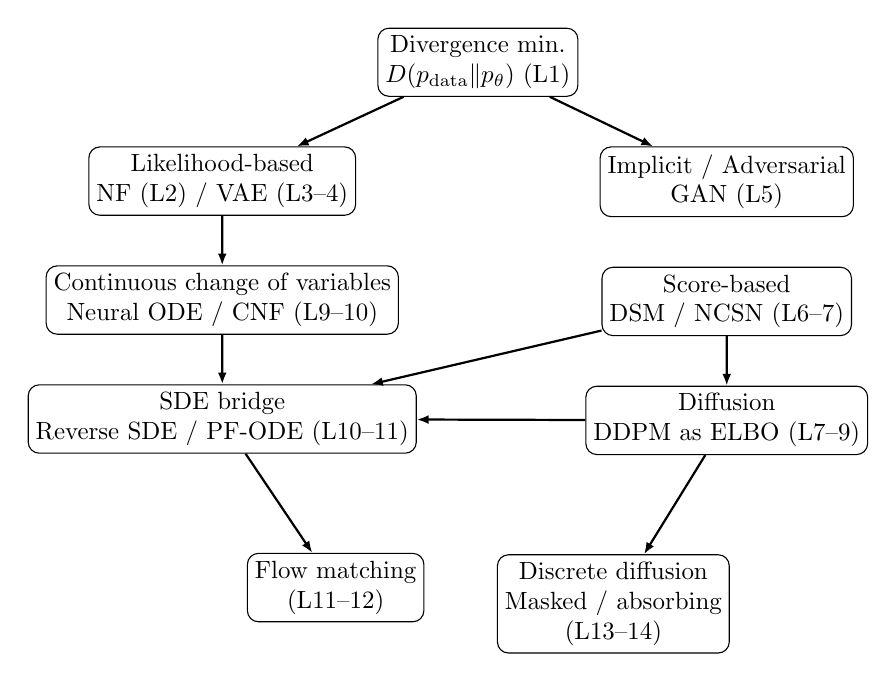
\begin{tikzpicture}[
		scale=0.9,
		transform shape,
		box/.style={draw, rounded corners, align=center, inner sep=3pt},
		arr/.style={-{Latex[length=1.5mm]}, thick},
		node distance=7mm and 3mm
	]
	\node[box] (div) {Divergence min.\\ $D(p_{\text{data}}\|p_\theta)$ (L1)};
	\node[box, below left=of div] (lik) {Likelihood-based\\ NF (L2) / VAE (L3--4)};
	\node[box, below right=of div] (imp) {Implicit / Adversarial\\ GAN (L5)};

	\node[box, below=of lik] (flows) {Continuous change of variables\\ Neural ODE / CNF (L9--10)};
	\node[box, below=of imp] (score) {Score-based\\ DSM / NCSN (L6--7)};

	\node[box, below=of flows] (sde) {SDE bridge\\ Reverse SDE / PF-ODE (L10--11)};
	\node[box, below=of score] (ddpm) {Diffusion\\ DDPM as ELBO (L7--9)};

	\node[box, below=14mm of sde, xshift=16mm] (fm) {Flow matching\\ (L11--12)};
	\node[box, below=14mm of ddpm, xshift=-16mm] (disc) {Discrete diffusion\\ Masked / absorbing\\ (L13--14)};

	\draw[arr] (div) -- (lik);
	\draw[arr] (div) -- (imp);
	\draw[arr] (lik) -- (flows);
	\draw[arr] (score) -- (ddpm);
	\draw[arr] (flows) -- (sde);
	\draw[arr] (ddpm) -- (sde);
	\draw[arr] (sde) -- (fm);
	\draw[arr] (ddpm) -- (disc);
	\draw[arr] (score) -- (sde);
	\end{tikzpicture}
\end{frame}
%=======
\begin{frame}{Comparison Cheat-Sheet: Part 1}
	\renewcommand{\arraystretch}{1.5}
	\center
	\begin{tabular}{lcccc}
		\hline
		\textbf{Family} & \textbf{Likelihood} & \textbf{Training} \\
		\hline
		AR & \checkmark & stable CE \\
		NF & \checkmark & tricky architecture \\
		VAE & lower bound & stable ELBO \\
		GAN & $\times$ & unstable/minimax \\
		Diffusion & bound / est. & stable \\
		FM / ODE & est. / bound & stable \\
		Discr. diff. & bound / CE-like & stable \\
		\hline
	\end{tabular}
\end{frame}
%=======
\begin{frame}{Comparison Cheat-Sheet: Part 2}
	\renewcommand{\arraystretch}{1.5}
	\center
	\begin{tabular}{lcccc}
	\hline
	\textbf{Family} & \textbf{Sampling} & \textbf{Best for} \\
	\hline
	AR & slow (sequential) & text / discrete \\
	NF & fast (1 step) & exact density, OOD \\
	VAE & fast (1 step) & latent modelling \\
	GAN & fast (1 step) & sharp images \\
	Diffusion & slow (many steps) & high fidelity + diversity \\
	FM / ODE & medium--fast & fewer steps + theory \\
	Discr. diff. & iterative & sequences + bidirectional gen \\
	\hline
	\end{tabular}
\end{frame}
%=======
\begin{frame}{Generative Learning Trilemma}
	\myfootnotewithlink{https://arxiv.org/abs/2112.07804}{Xiao Z., Kreis K., Vahdat A. Tackling the generative learning trilemma with denoising diffusion GANs, 2021}
	\begin{figure}
		\includegraphics[width=0.7\linewidth]{../lecture14/figs/trilemma}
	\end{figure}
\end{frame}
%=======
\begin{frame}{Generative Learning Trilemma}
	\begin{block}{Rule of Thumb}
	\small
		\begin{itemize}
			\item \textbf{Likelihood $\;\&\;$ Coverage} $\Rightarrow$ 
			\textbf{AR / NF}  
			\hfill exact density, no mode dropping, \textit{slow sampling}

			\item \textbf{Likelihood $\;\&\;$ Fast Sampling} $\Rightarrow$ 
			\textbf{VAE}  
			\hfill tractable bound, fast, \textit{blurry samples}

			\item \textbf{Sample Quality $\;\&\;$ Fast Sampling} $\Rightarrow$ 
			\textbf{GAN}  
			\hfill sharp samples, \textit{no likelihood, mode collapse}

			\item \textbf{Quality $\;\&\;$ Coverage} $\Rightarrow$ 
			\textbf{Diffusion}  
			\hfill stable training, high fidelity, \textit{slow sampling}

			\item \textbf{Quality $\;\&\;$ Faster Sampling} $\Rightarrow$ 
			\textbf{FM / ODE}  
			\hfill fewer steps, continuous flows, \textit{approx.\ likelihood}

			\item \textbf{Discrete Structure $\;\&\;$ Coverage} $\Rightarrow$ 
			\textbf{Discrete Diffusion}  
			\hfill stable CE training, parallel denoising, \textit{iterative decoding}
		\end{itemize}
	\end{block}
\end{frame}
%=======
\begin{frame}{Summary}
	\begin{itemize}
		\item For sequences, the forward process of discrete diffusionfactorize over positions, but
		reverse process (the model $\pt$) conditions on the whole context.
		\vfill
		\item In the absorbing case, tokens are either unchanged or masked; so only masked tokens contribute to the ELBO loss.
		\vfill
		\item The discrete ELBO reduces to a MLM objective.
		\vfill
		\item Reparameterizing time by the mask rate $\lambda\in[0,1]$ yields a continuous mixture of MLM losses.
		\vfill
		\item MDLM sampling performs iterative parallel refinement from fully masked to fully unmasked sequences.
		\vfill
		\item No generative model is strictly better than all others: different methods occupy different corners of the generative learning trilemma and come with unavoidable disadvantages.
	\end{itemize}
\end{frame}
%=======

\end{document}
